\documentclass[twoside]{book}

% Packages required by doxygen
\usepackage{fixltx2e}
\usepackage{calc}
\usepackage{doxygen}
\usepackage[export]{adjustbox} % also loads graphicx
\usepackage{graphicx}
\usepackage[utf8]{inputenc}
\usepackage{makeidx}
\usepackage{multicol}
\usepackage{multirow}
\PassOptionsToPackage{warn}{textcomp}
\usepackage{textcomp}
\usepackage[nointegrals]{wasysym}
\usepackage[table]{xcolor}

% Font selection
\usepackage[T1]{fontenc}
\usepackage[scaled=.90]{helvet}
\usepackage{courier}
\usepackage{amssymb}
\usepackage{sectsty}
\renewcommand{\familydefault}{\sfdefault}
\allsectionsfont{%
  \fontseries{bc}\selectfont%
  \color{darkgray}%
}
\renewcommand{\DoxyLabelFont}{%
  \fontseries{bc}\selectfont%
  \color{darkgray}%
}
\newcommand{\+}{\discretionary{\mbox{\scriptsize$\hookleftarrow$}}{}{}}

% Page & text layout
\usepackage{geometry}
\geometry{%
  a4paper,%
  top=2.5cm,%
  bottom=2.5cm,%
  left=2.5cm,%
  right=2.5cm%
}
\tolerance=750
\hfuzz=15pt
\hbadness=750
\setlength{\emergencystretch}{15pt}
\setlength{\parindent}{0cm}
\setlength{\parskip}{3ex plus 2ex minus 2ex}
\makeatletter
\renewcommand{\paragraph}{%
  \@startsection{paragraph}{4}{0ex}{-1.0ex}{1.0ex}{%
    \normalfont\normalsize\bfseries\SS@parafont%
  }%
}
\renewcommand{\subparagraph}{%
  \@startsection{subparagraph}{5}{0ex}{-1.0ex}{1.0ex}{%
    \normalfont\normalsize\bfseries\SS@subparafont%
  }%
}
\makeatother

% Headers & footers
\usepackage{fancyhdr}
\pagestyle{fancyplain}
\fancyhead[LE]{\fancyplain{}{\bfseries\thepage}}
\fancyhead[CE]{\fancyplain{}{}}
\fancyhead[RE]{\fancyplain{}{\bfseries\leftmark}}
\fancyhead[LO]{\fancyplain{}{\bfseries\rightmark}}
\fancyhead[CO]{\fancyplain{}{}}
\fancyhead[RO]{\fancyplain{}{\bfseries\thepage}}
\fancyfoot[LE]{\fancyplain{}{}}
\fancyfoot[CE]{\fancyplain{}{}}
\fancyfoot[RE]{\fancyplain{}{\bfseries\scriptsize Generated by Doxygen }}
\fancyfoot[LO]{\fancyplain{}{\bfseries\scriptsize Generated by Doxygen }}
\fancyfoot[CO]{\fancyplain{}{}}
\fancyfoot[RO]{\fancyplain{}{}}
\renewcommand{\footrulewidth}{0.4pt}
\renewcommand{\chaptermark}[1]{%
  \markboth{#1}{}%
}
\renewcommand{\sectionmark}[1]{%
  \markright{\thesection\ #1}%
}

% Indices & bibliography
\usepackage{natbib}
\usepackage[titles]{tocloft}
\setcounter{tocdepth}{3}
\setcounter{secnumdepth}{5}
\makeindex

% Custom commands
\newcommand{\clearemptydoublepage}{%
  \newpage{\pagestyle{empty}\cleardoublepage}%
}

\usepackage{caption}
\captionsetup{labelsep=space,justification=centering,font={bf},singlelinecheck=off,skip=4pt,position=top}

%===== C O N T E N T S =====

\begin{document}

% Titlepage & ToC
\pagenumbering{alph}
\begin{titlepage}
\vspace*{7cm}
\begin{center}%
{\Large t\+A\+Itris \\[1ex]\large v1.\+0 }\\
\vspace*{1cm}
{\large Generated by Doxygen 1.8.13}\\
\end{center}
\end{titlepage}
\clearemptydoublepage
\pagenumbering{roman}
\tableofcontents
\clearemptydoublepage
\pagenumbering{arabic}

%--- Begin generated contents ---
\chapter{Data Structure Index}
\section{Data Structures}
Here are the data structures with brief descriptions\+:\begin{DoxyCompactList}
\item\contentsline{section}{\textbf{ list} }{\pageref{structlist}}{}
\item\contentsline{section}{\textbf{ list\+\_\+node} }{\pageref{structlist__node}}{}
\end{DoxyCompactList}

\chapter{File Index}
\section{File List}
Here is a list of all files with brief descriptions\+:\begin{DoxyCompactList}
\item\contentsline{section}{src/\textbf{ t\+A\+Itris.\+c} \\*Main file }{\pageref{tAItris_8c}}{}
\item\contentsline{section}{src/ai/genetic/\textbf{ core.\+c} \\*Core of the genetic algorithm }{\pageref{core_8c}}{}
\item\contentsline{section}{src/ai/genetic/\textbf{ core.\+h} \\*Core of the genetic algorithm }{\pageref{core_8h}}{}
\item\contentsline{section}{src/ai/genetic/\textbf{ engine.\+c} \\*Engine for the genetic algorithm }{\pageref{engine_8c}}{}
\item\contentsline{section}{src/ai/genetic/\textbf{ engine.\+h} \\*Engine for the genetic algorithm }{\pageref{engine_8h}}{}
\item\contentsline{section}{src/ai/genetic/\textbf{ tools.\+c} \\*Tools for the genetic algorithm }{\pageref{tools_8c}}{}
\item\contentsline{section}{src/ai/genetic/\textbf{ tools.\+h} \\*Tools for the genetic algorithm }{\pageref{tools_8h}}{}
\item\contentsline{section}{src/debug/\textbf{ debug.\+h} \\*Debug }{\pageref{debug_8h}}{}
\item\contentsline{section}{src/debug/engine/\textbf{ debug\+\_\+state.\+c} \\*Debug state }{\pageref{debug__state_8c}}{}
\item\contentsline{section}{src/debug/engine/\textbf{ debug\+\_\+state.\+h} \\*Debug state }{\pageref{debug__state_8h}}{}
\item\contentsline{section}{src/engine/\textbf{ angle.\+h} \\*Angle }{\pageref{angle_8h}}{}
\item\contentsline{section}{src/engine/\textbf{ board.\+c} \\*\doxyref{Board}{p.}{structBoard} }{\pageref{board_8c}}{}
\item\contentsline{section}{src/engine/\textbf{ board.\+h} \\*\doxyref{Board}{p.}{structBoard} }{\pageref{board_8h}}{}
\item\contentsline{section}{src/engine/\textbf{ cell.\+h} \\*Cell }{\pageref{cell_8h}}{}
\item\contentsline{section}{src/engine/\textbf{ input.\+h} \\*Input }{\pageref{input_8h}}{}
\item\contentsline{section}{src/engine/\textbf{ motion.\+c} \\*Motion }{\pageref{motion_8c}}{}
\item\contentsline{section}{src/engine/\textbf{ motion.\+h} \\*Motion }{\pageref{motion_8h}}{}
\item\contentsline{section}{src/engine/\textbf{ score.\+c} \\*Scoring system }{\pageref{score_8c}}{}
\item\contentsline{section}{src/engine/\textbf{ score.\+h} \\*Scoring system }{\pageref{score_8h}}{}
\item\contentsline{section}{src/engine/\textbf{ state.\+c} \\*\doxyref{State}{p.}{structState} }{\pageref{state_8c}}{}
\item\contentsline{section}{src/engine/\textbf{ state.\+h} \\*\doxyref{State}{p.}{structState} }{\pageref{state_8h}}{}
\item\contentsline{section}{src/engine/piece/\textbf{ piece.\+c} \\*\doxyref{Piece}{p.}{structPiece} }{\pageref{piece_8c}}{}
\item\contentsline{section}{src/engine/piece/\textbf{ piece.\+h} \\*\doxyref{Piece}{p.}{structPiece} }{\pageref{piece_8h}}{}
\item\contentsline{section}{src/engine/piece/\textbf{ piece\+\_\+queue.\+c} \\*\doxyref{Piece}{p.}{structPiece} queue }{\pageref{piece__queue_8c}}{}
\item\contentsline{section}{src/engine/piece/\textbf{ piece\+\_\+queue.\+h} \\*\doxyref{Piece}{p.}{structPiece} queue }{\pageref{piece__queue_8h}}{}
\item\contentsline{section}{src/engine/piece/\textbf{ piece\+\_\+shape.\+h} \\*\doxyref{Piece}{p.}{structPiece} shape }{\pageref{piece__shape_8h}}{}
\item\contentsline{section}{src/engine/piece/\textbf{ piece\+\_\+type.\+h} \\*\doxyref{Piece}{p.}{structPiece} type }{\pageref{piece__type_8h}}{}
\item\contentsline{section}{src/engine/piece/\textbf{ seven\+\_\+bag.\+c} \\*7-\/\+Bag generator }{\pageref{seven__bag_8c}}{}
\item\contentsline{section}{src/engine/piece/\textbf{ seven\+\_\+bag.\+h} \\*7-\/\+Bag generator }{\pageref{seven__bag_8h}}{}
\item\contentsline{section}{src/utils/\textbf{ ansi\+\_\+code.\+h} \\*A\+N\+SI escape code }{\pageref{ansi__code_8h}}{}
\item\contentsline{section}{src/utils/\textbf{ random.\+h} \\*Random number generation }{\pageref{random_8h}}{}
\item\contentsline{section}{src/utils/\textbf{ safe\+\_\+op.\+h} \\*Safe operations }{\pageref{safe__op_8h}}{}
\end{DoxyCompactList}

\chapter{Data Structure Documentation}
\section{Ai\+Coefs Struct Reference}
\label{structAiCoefs}\index{Ai\+Coefs@{Ai\+Coefs}}


{\ttfamily \#include $<$engine.\+h$>$}

\subsection*{Data Fields}
\begin{DoxyCompactItemize}
\item 
double \textbf{ agg\+\_\+height}
\item 
double \textbf{ holes}
\item 
double \textbf{ clears}
\item 
double \textbf{ bumpiness}
\end{DoxyCompactItemize}


\subsection{Field Documentation}
\mbox{\label{structAiCoefs_a0691df3d11342de203475e6993146f76}} 
\index{Ai\+Coefs@{Ai\+Coefs}!agg\+\_\+height@{agg\+\_\+height}}
\index{agg\+\_\+height@{agg\+\_\+height}!Ai\+Coefs@{Ai\+Coefs}}
\subsubsection{agg\+\_\+height}
{\footnotesize\ttfamily double agg\+\_\+height}

\mbox{\label{structAiCoefs_a7a634ecd67e00fc4b19a86046ad95154}} 
\index{Ai\+Coefs@{Ai\+Coefs}!bumpiness@{bumpiness}}
\index{bumpiness@{bumpiness}!Ai\+Coefs@{Ai\+Coefs}}
\subsubsection{bumpiness}
{\footnotesize\ttfamily double bumpiness}

\mbox{\label{structAiCoefs_a7e11e19ab08623daaac58bd77d5f80c4}} 
\index{Ai\+Coefs@{Ai\+Coefs}!clears@{clears}}
\index{clears@{clears}!Ai\+Coefs@{Ai\+Coefs}}
\subsubsection{clears}
{\footnotesize\ttfamily double clears}

\mbox{\label{structAiCoefs_acf9e4d84dfc5d65f5a85fc4dc3a5fadb}} 
\index{Ai\+Coefs@{Ai\+Coefs}!holes@{holes}}
\index{holes@{holes}!Ai\+Coefs@{Ai\+Coefs}}
\subsubsection{holes}
{\footnotesize\ttfamily double holes}



The documentation for this struct was generated from the following file\+:\begin{DoxyCompactItemize}
\item 
src/ai/genetic/\textbf{ engine.\+h}\end{DoxyCompactItemize}

\section{Board Struct Reference}
\label{structBoard}\index{Board@{Board}}


{\ttfamily \#include $<$board.\+h$>$}

\subsection*{Data Fields}
\begin{DoxyCompactItemize}
\item 
int \textbf{ width}
\item 
int \textbf{ height}
\item 
\textbf{ Cell} $\ast$ \textbf{ cells}
\end{DoxyCompactItemize}


\subsection{Field Documentation}
\mbox{\label{structBoard_a4b2f78a0197c8d34d405912888acfe7c}} 
\index{Board@{Board}!cells@{cells}}
\index{cells@{cells}!Board@{Board}}
\subsubsection{cells}
{\footnotesize\ttfamily \textbf{ Cell}$\ast$ cells}

\mbox{\label{structBoard_ad12fc34ce789bce6c8a05d8a17138534}} 
\index{Board@{Board}!height@{height}}
\index{height@{height}!Board@{Board}}
\subsubsection{height}
{\footnotesize\ttfamily int height}

\mbox{\label{structBoard_a2474a5474cbff19523a51eb1de01cda4}} 
\index{Board@{Board}!width@{width}}
\index{width@{width}!Board@{Board}}
\subsubsection{width}
{\footnotesize\ttfamily int width}



The documentation for this struct was generated from the following file\+:\begin{DoxyCompactItemize}
\item 
src/engine/\textbf{ board.\+h}\end{DoxyCompactItemize}

\section{Piece Struct Reference}
\label{structPiece}\index{Piece@{Piece}}


{\ttfamily \#include $<$piece.\+h$>$}



Collaboration diagram for Piece\+:
\nopagebreak
\begin{figure}[H]
\begin{center}
\leavevmode
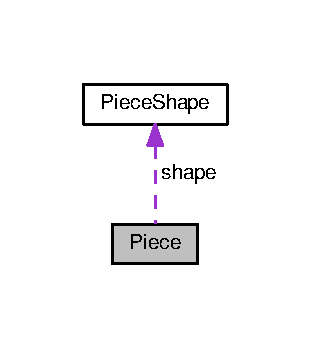
\includegraphics[width=149pt]{structPiece__coll__graph}
\end{center}
\end{figure}
\subsection*{Data Fields}
\begin{DoxyCompactItemize}
\item 
\textbf{ Piece\+Type} \textbf{ type}
\item 
const \textbf{ Piece\+Shape} $\ast$ \textbf{ shape}
\item 
int \textbf{ x}
\item 
int \textbf{ y}
\item 
\textbf{ Angle} \textbf{ angle}
\end{DoxyCompactItemize}


\subsection{Field Documentation}
\mbox{\label{structPiece_ada2a4e7499e58efcb049762e1d961c4e}} 
\index{Piece@{Piece}!angle@{angle}}
\index{angle@{angle}!Piece@{Piece}}
\subsubsection{angle}
{\footnotesize\ttfamily \textbf{ Angle} angle}

\mbox{\label{structPiece_ad98d3b155e2d7b43f0eaacdad5465829}} 
\index{Piece@{Piece}!shape@{shape}}
\index{shape@{shape}!Piece@{Piece}}
\subsubsection{shape}
{\footnotesize\ttfamily const \textbf{ Piece\+Shape}$\ast$ shape}

\mbox{\label{structPiece_a7bbc30d6dbbc70180417e3bb006b52e9}} 
\index{Piece@{Piece}!type@{type}}
\index{type@{type}!Piece@{Piece}}
\subsubsection{type}
{\footnotesize\ttfamily \textbf{ Piece\+Type} type}

\mbox{\label{structPiece_a6150e0515f7202e2fb518f7206ed97dc}} 
\index{Piece@{Piece}!x@{x}}
\index{x@{x}!Piece@{Piece}}
\subsubsection{x}
{\footnotesize\ttfamily int x}

\mbox{\label{structPiece_a0a2f84ed7838f07779ae24c5a9086d33}} 
\index{Piece@{Piece}!y@{y}}
\index{y@{y}!Piece@{Piece}}
\subsubsection{y}
{\footnotesize\ttfamily int y}



The documentation for this struct was generated from the following file\+:\begin{DoxyCompactItemize}
\item 
src/engine/piece/\textbf{ piece.\+h}\end{DoxyCompactItemize}

\section{Piece\+Queue Struct Reference}
\label{structPieceQueue}\index{Piece\+Queue@{Piece\+Queue}}


{\ttfamily \#include $<$piece\+\_\+queue.\+h$>$}

\subsection*{Data Fields}
\begin{DoxyCompactItemize}
\item 
size\+\_\+t \textbf{ length}
\item 
\textbf{ Piece\+Type} $\ast$ \textbf{ data}
\end{DoxyCompactItemize}


\subsection{Field Documentation}
\mbox{\label{structPieceQueue_aba4149dd7852c6f12ca5b26712592e3c}} 
\index{Piece\+Queue@{Piece\+Queue}!data@{data}}
\index{data@{data}!Piece\+Queue@{Piece\+Queue}}
\subsubsection{data}
{\footnotesize\ttfamily \textbf{ Piece\+Type}$\ast$ data}

\mbox{\label{structPieceQueue_ae809d5359ac030c60a30a8f0b2294b82}} 
\index{Piece\+Queue@{Piece\+Queue}!length@{length}}
\index{length@{length}!Piece\+Queue@{Piece\+Queue}}
\subsubsection{length}
{\footnotesize\ttfamily size\+\_\+t length}



The documentation for this struct was generated from the following file\+:\begin{DoxyCompactItemize}
\item 
src/engine/piece/\textbf{ piece\+\_\+queue.\+h}\end{DoxyCompactItemize}

\section{Piece\+Shape Struct Reference}
\label{structPieceShape}\index{Piece\+Shape@{Piece\+Shape}}


{\ttfamily \#include $<$piece\+\_\+shape.\+h$>$}

\subsection*{Data Fields}
\begin{DoxyCompactItemize}
\item 
int \textbf{ shape} [\textbf{ A\+N\+G\+L\+E\+\_\+\+E\+S\+I\+ZE}][\textbf{ P\+I\+E\+C\+E\+\_\+\+S\+H\+A\+P\+E\+\_\+\+H\+E\+I\+G\+HT}][\textbf{ P\+I\+E\+C\+E\+\_\+\+S\+H\+A\+P\+E\+\_\+\+W\+I\+D\+TH}]
\item 
\textbf{ Cell} \textbf{ fill}
\end{DoxyCompactItemize}


\subsection{Field Documentation}
\mbox{\label{structPieceShape_a56827e5a472a2fa6b604a110d7398aaf}} 
\index{Piece\+Shape@{Piece\+Shape}!fill@{fill}}
\index{fill@{fill}!Piece\+Shape@{Piece\+Shape}}
\subsubsection{fill}
{\footnotesize\ttfamily \textbf{ Cell} fill}

\mbox{\label{structPieceShape_ad2366aa5b082ad2eab949ca0529bf186}} 
\index{Piece\+Shape@{Piece\+Shape}!shape@{shape}}
\index{shape@{shape}!Piece\+Shape@{Piece\+Shape}}
\subsubsection{shape}
{\footnotesize\ttfamily int shape[\textbf{ A\+N\+G\+L\+E\+\_\+\+E\+S\+I\+ZE}][\textbf{ P\+I\+E\+C\+E\+\_\+\+S\+H\+A\+P\+E\+\_\+\+H\+E\+I\+G\+HT}][\textbf{ P\+I\+E\+C\+E\+\_\+\+S\+H\+A\+P\+E\+\_\+\+W\+I\+D\+TH}]}



The documentation for this struct was generated from the following file\+:\begin{DoxyCompactItemize}
\item 
src/engine/piece/\textbf{ piece\+\_\+shape.\+h}\end{DoxyCompactItemize}

\section{State Struct Reference}
\label{structState}\index{State@{State}}


{\ttfamily \#include $<$state.\+h$>$}



Collaboration diagram for State\+:
\nopagebreak
\begin{figure}[H]
\begin{center}
\leavevmode
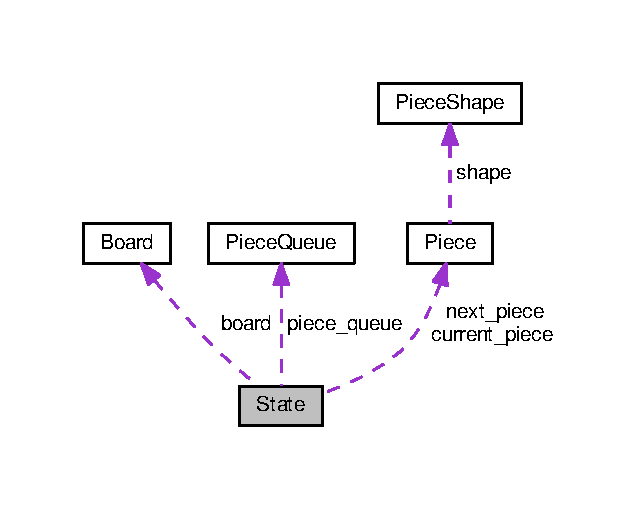
\includegraphics[width=306pt]{structState__coll__graph}
\end{center}
\end{figure}
\subsection*{Data Fields}
\begin{DoxyCompactItemize}
\item 
unsigned int \textbf{ score}
\item 
unsigned int \textbf{ level}
\item 
unsigned int \textbf{ broken\+\_\+lines}
\item 
unsigned int \textbf{ step}
\item 
unsigned int \textbf{ input\+\_\+counts}
\item 
\textbf{ Board} $\ast$ \textbf{ board}
\item 
\textbf{ Piece\+Queue} $\ast$ \textbf{ piece\+\_\+queue}
\item 
size\+\_\+t \textbf{ piece\+\_\+queue\+\_\+index}
\item 
\textbf{ Piece} $\ast$ \textbf{ current\+\_\+piece}
\item 
\textbf{ Piece} $\ast$ \textbf{ next\+\_\+piece}
\end{DoxyCompactItemize}


\subsection{Field Documentation}
\mbox{\label{structState_ab8dad7d3cb14e06a506084453a9cf527}} 
\index{State@{State}!board@{board}}
\index{board@{board}!State@{State}}
\subsubsection{board}
{\footnotesize\ttfamily \textbf{ Board}$\ast$ board}

\mbox{\label{structState_a67fc108b56c9238ce197b470af1f1727}} 
\index{State@{State}!broken\+\_\+lines@{broken\+\_\+lines}}
\index{broken\+\_\+lines@{broken\+\_\+lines}!State@{State}}
\subsubsection{broken\+\_\+lines}
{\footnotesize\ttfamily unsigned int broken\+\_\+lines}

\mbox{\label{structState_a720152f0ad7b57a077424a1a48efcf7e}} 
\index{State@{State}!current\+\_\+piece@{current\+\_\+piece}}
\index{current\+\_\+piece@{current\+\_\+piece}!State@{State}}
\subsubsection{current\+\_\+piece}
{\footnotesize\ttfamily \textbf{ Piece}$\ast$ current\+\_\+piece}

\mbox{\label{structState_a0d74c170ea3f963a63b02b037e0edc6c}} 
\index{State@{State}!input\+\_\+counts@{input\+\_\+counts}}
\index{input\+\_\+counts@{input\+\_\+counts}!State@{State}}
\subsubsection{input\+\_\+counts}
{\footnotesize\ttfamily unsigned int input\+\_\+counts}

\mbox{\label{structState_a9082f945c1d289684d0bcd51ee08e11e}} 
\index{State@{State}!level@{level}}
\index{level@{level}!State@{State}}
\subsubsection{level}
{\footnotesize\ttfamily unsigned int level}

\mbox{\label{structState_a0be8ae11bca3b397007b6be567b13711}} 
\index{State@{State}!next\+\_\+piece@{next\+\_\+piece}}
\index{next\+\_\+piece@{next\+\_\+piece}!State@{State}}
\subsubsection{next\+\_\+piece}
{\footnotesize\ttfamily \textbf{ Piece}$\ast$ next\+\_\+piece}

\mbox{\label{structState_a03cfc54cf110d49f618178d7c6696977}} 
\index{State@{State}!piece\+\_\+queue@{piece\+\_\+queue}}
\index{piece\+\_\+queue@{piece\+\_\+queue}!State@{State}}
\subsubsection{piece\+\_\+queue}
{\footnotesize\ttfamily \textbf{ Piece\+Queue}$\ast$ piece\+\_\+queue}

\mbox{\label{structState_a00d61210bd561ca12fe3cbea231802bf}} 
\index{State@{State}!piece\+\_\+queue\+\_\+index@{piece\+\_\+queue\+\_\+index}}
\index{piece\+\_\+queue\+\_\+index@{piece\+\_\+queue\+\_\+index}!State@{State}}
\subsubsection{piece\+\_\+queue\+\_\+index}
{\footnotesize\ttfamily size\+\_\+t piece\+\_\+queue\+\_\+index}

\mbox{\label{structState_a9dffb288f0f2281a0b9abbd8efaa5a18}} 
\index{State@{State}!score@{score}}
\index{score@{score}!State@{State}}
\subsubsection{score}
{\footnotesize\ttfamily unsigned int score}

\mbox{\label{structState_aff48805b5e25bfa4af93ea7e44481596}} 
\index{State@{State}!step@{step}}
\index{step@{step}!State@{State}}
\subsubsection{step}
{\footnotesize\ttfamily unsigned int step}



The documentation for this struct was generated from the following file\+:\begin{DoxyCompactItemize}
\item 
src/engine/\textbf{ state.\+h}\end{DoxyCompactItemize}

\chapter{File Documentation}
\section{src/ai/genetic/core.c File Reference}
\label{core_8c}\index{src/ai/genetic/core.\+c@{src/ai/genetic/core.\+c}}


Core of the genetic algorithm.  


{\ttfamily \#include \char`\"{}core.\+h\char`\"{}}\newline
Include dependency graph for core.\+c\+:
\nopagebreak
\begin{figure}[H]
\begin{center}
\leavevmode
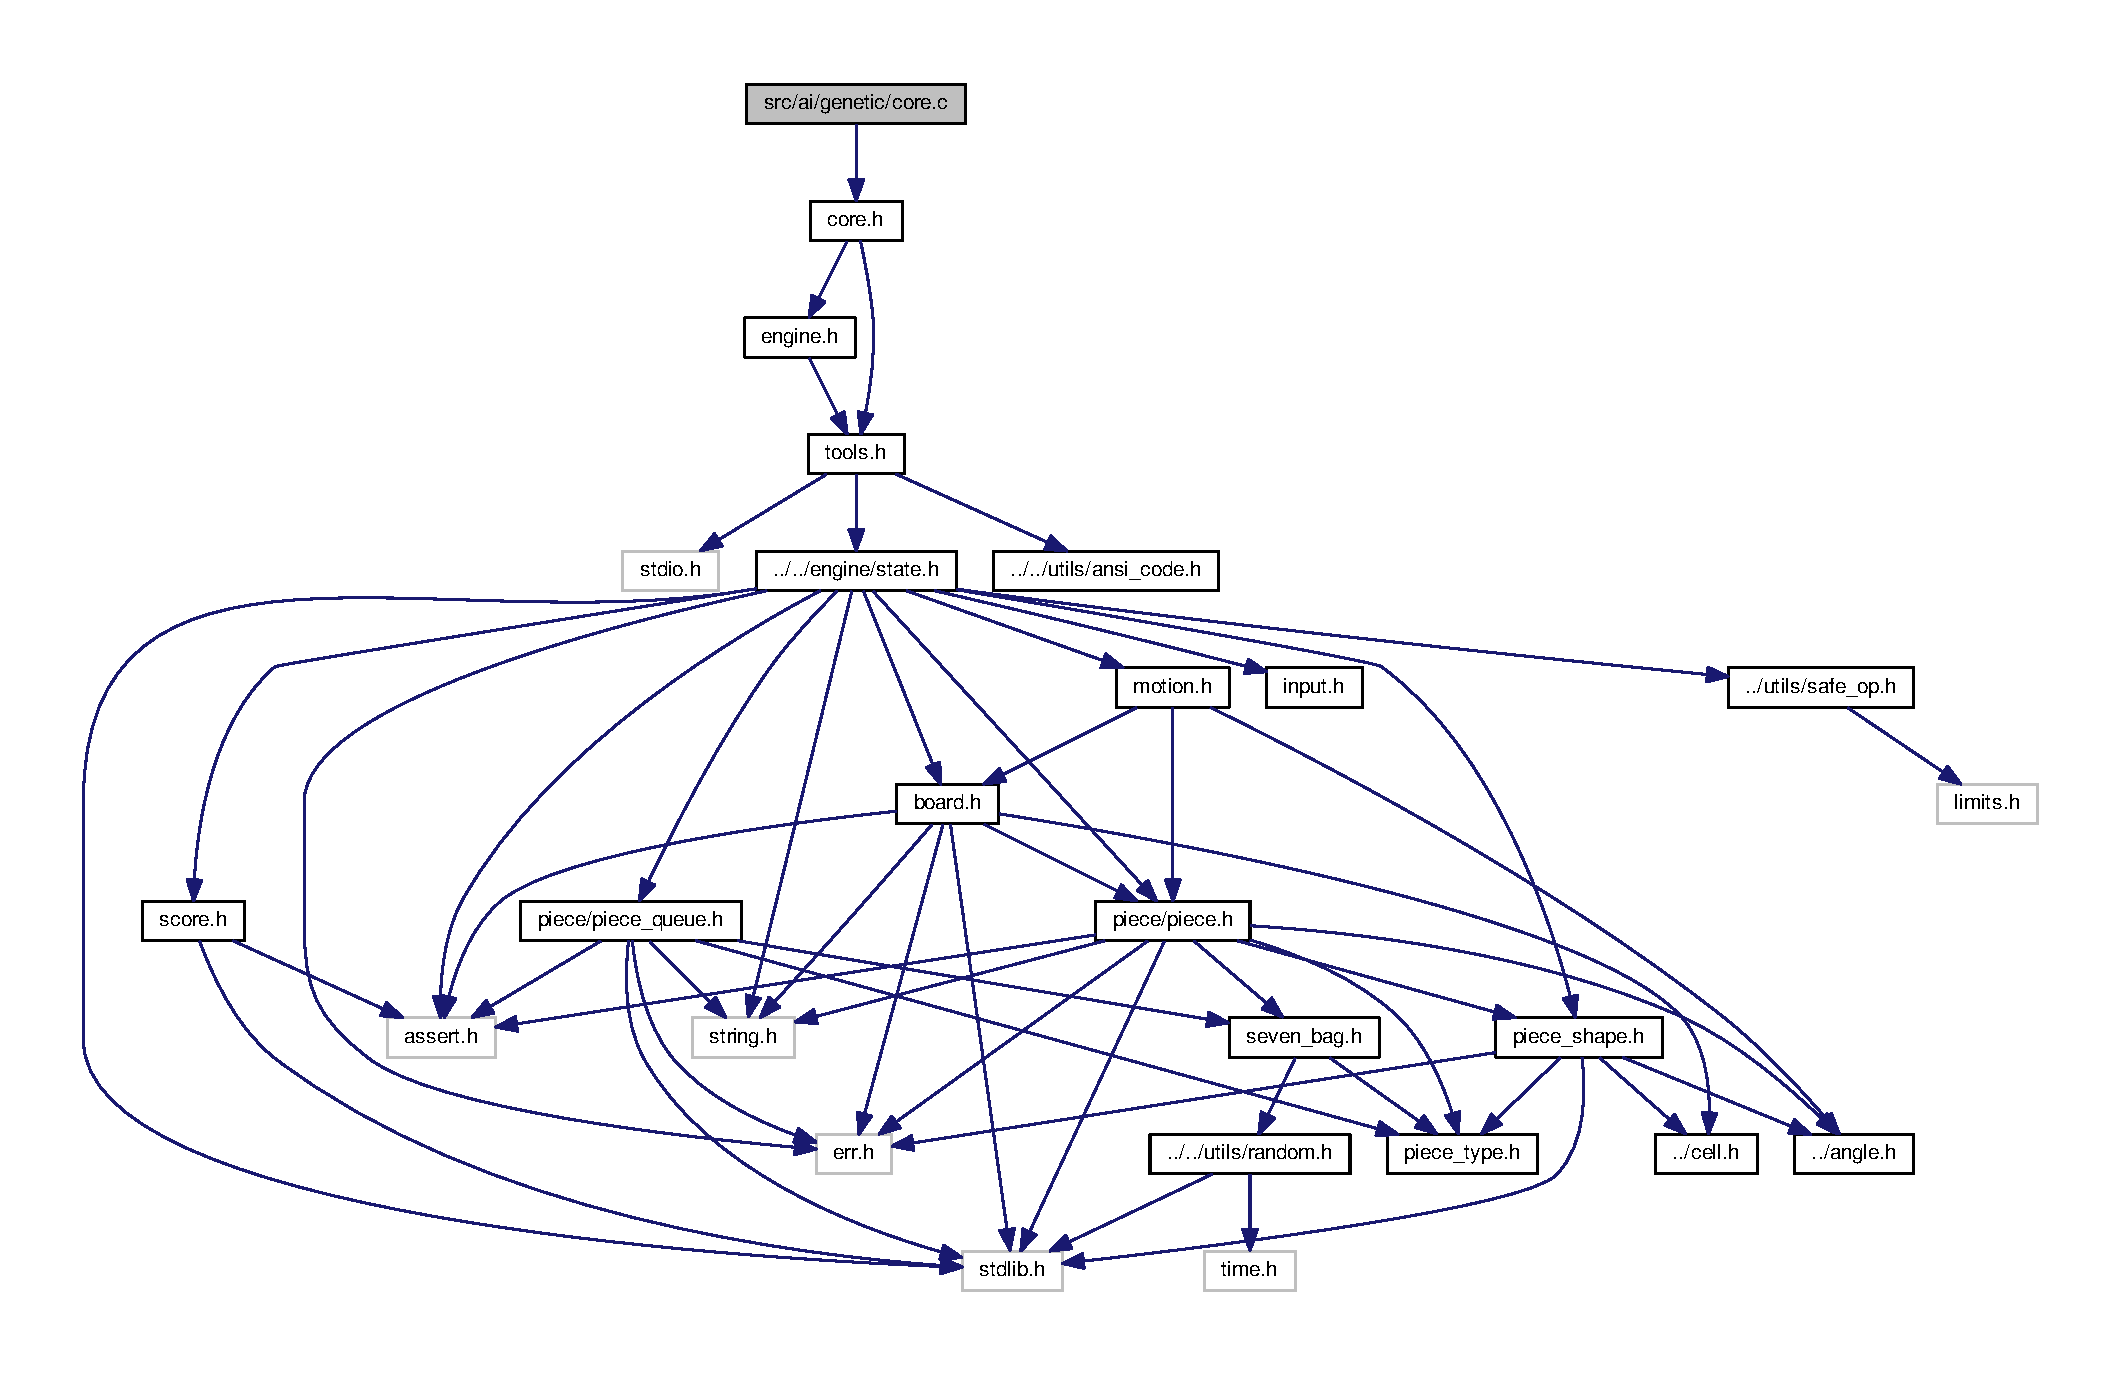
\includegraphics[width=350pt]{core_8c__incl}
\end{center}
\end{figure}
\subsection*{Functions}
\begin{DoxyCompactItemize}
\item 
void \textbf{ genetic\+\_\+show\+\_\+stats} (\textbf{ State} $\ast$state)
\end{DoxyCompactItemize}


\subsection{Detailed Description}
Core of the genetic algorithm. 

\begin{DoxyAuthor}{Author}
S4\+Master\+Race 
\end{DoxyAuthor}
\begin{DoxyVersion}{Version}
2.\+0 
\end{DoxyVersion}


\subsection{Function Documentation}
\mbox{\label{core_8c_a471131fbd6fb873da1e9e9e34866f35b}} 
\index{core.\+c@{core.\+c}!genetic\+\_\+show\+\_\+stats@{genetic\+\_\+show\+\_\+stats}}
\index{genetic\+\_\+show\+\_\+stats@{genetic\+\_\+show\+\_\+stats}!core.\+c@{core.\+c}}
\subsubsection{genetic\+\_\+show\+\_\+stats()}
{\footnotesize\ttfamily void genetic\+\_\+show\+\_\+stats (\begin{DoxyParamCaption}\item[{\textbf{ State} $\ast$}]{state }\end{DoxyParamCaption})}


\section{src/ai/genetic/core.h File Reference}
\label{core_8h}\index{src/ai/genetic/core.\+h@{src/ai/genetic/core.\+h}}


Core of the genetic algorithm.  


{\ttfamily \#include \char`\"{}engine.\+h\char`\"{}}\newline
{\ttfamily \#include \char`\"{}tools.\+h\char`\"{}}\newline
Include dependency graph for core.\+h\+:
\nopagebreak
\begin{figure}[H]
\begin{center}
\leavevmode
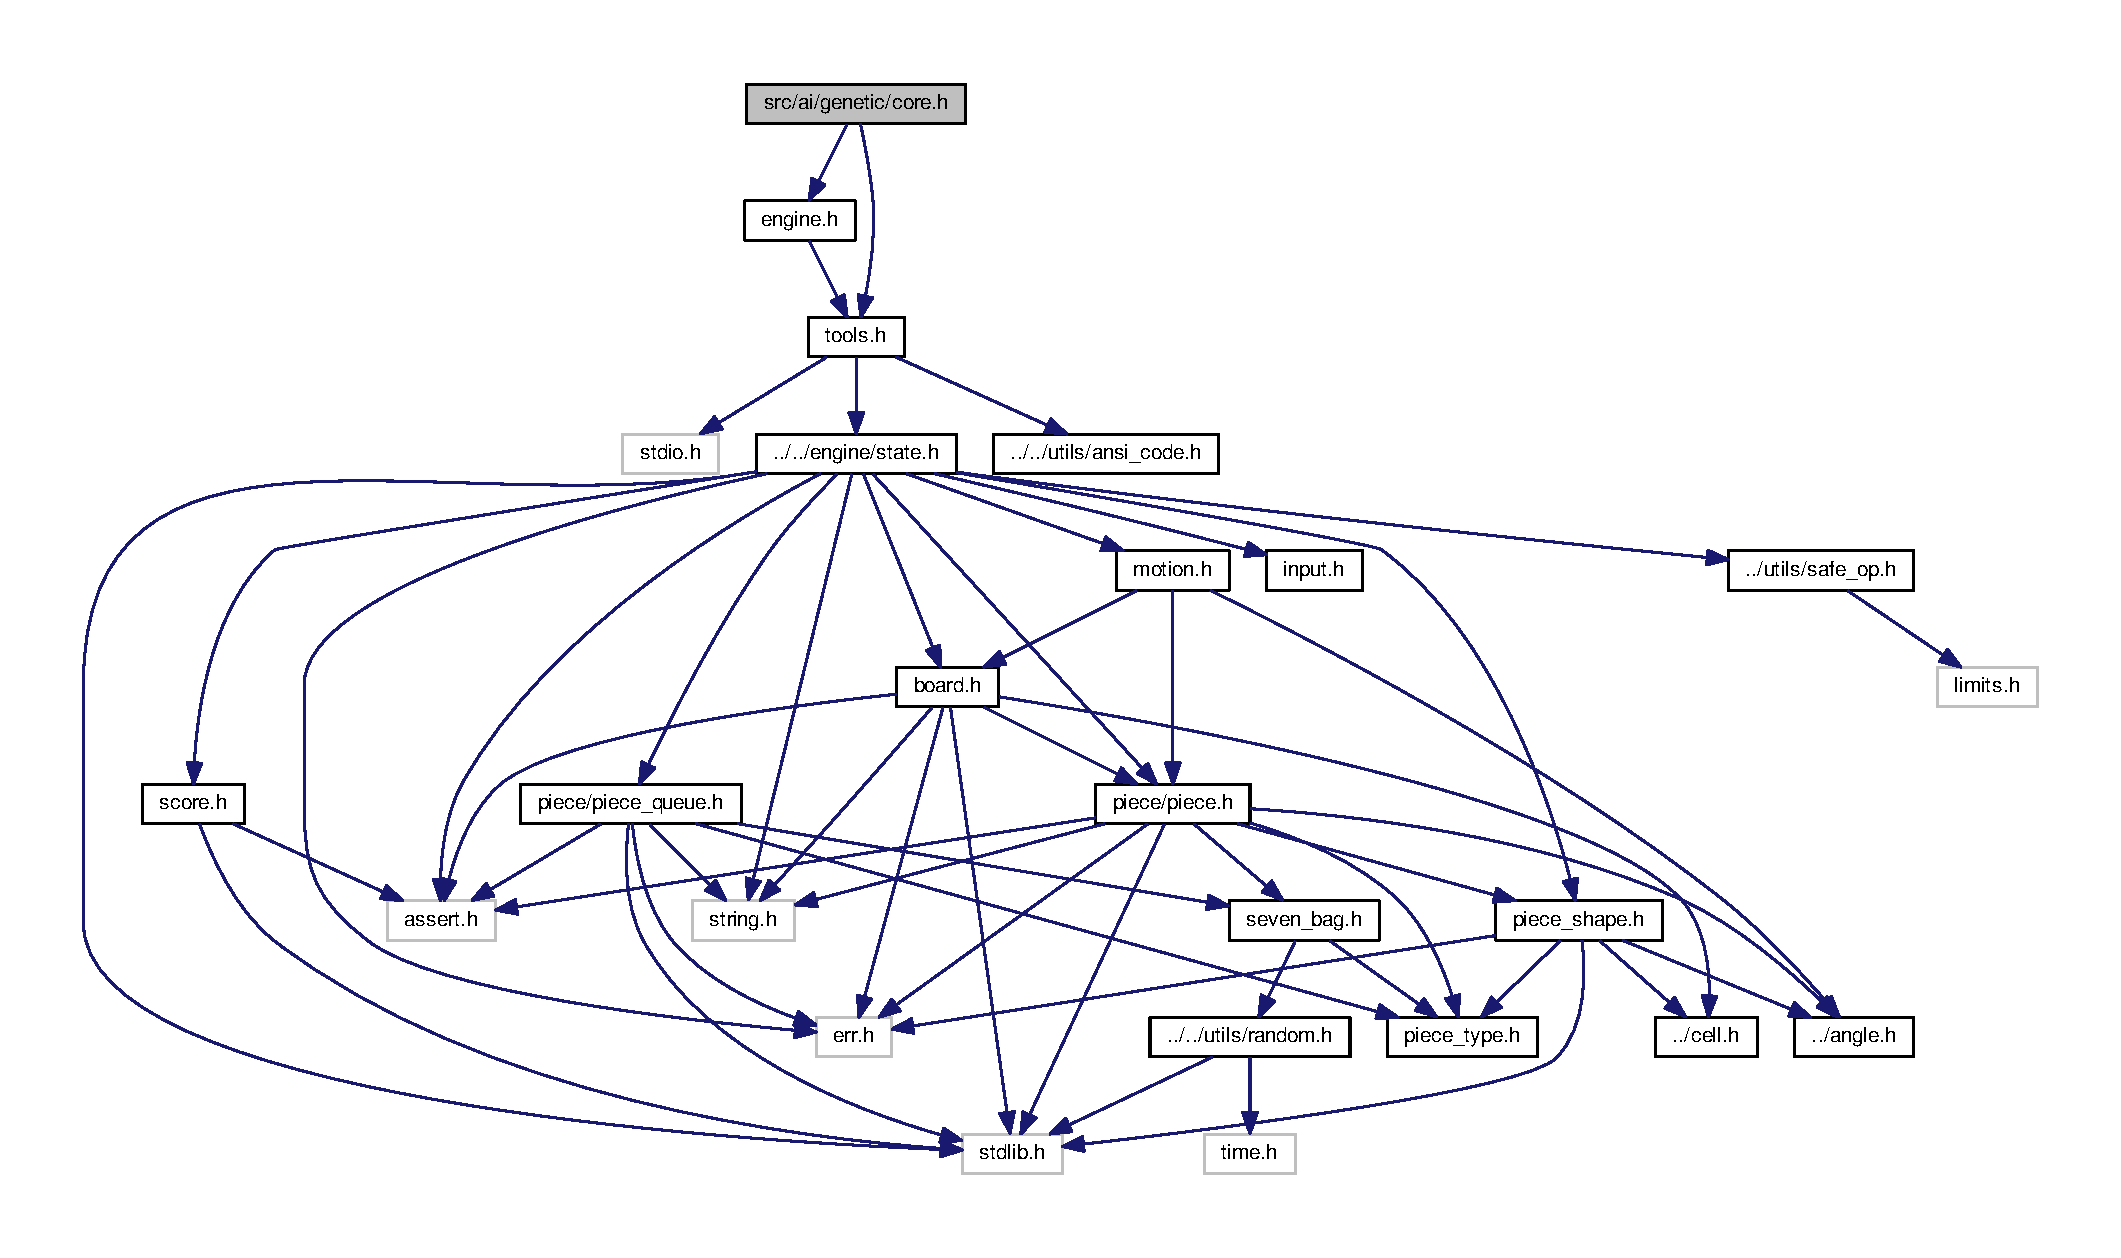
\includegraphics[width=350pt]{core_8h__incl}
\end{center}
\end{figure}
This graph shows which files directly or indirectly include this file\+:
\nopagebreak
\begin{figure}[H]
\begin{center}
\leavevmode
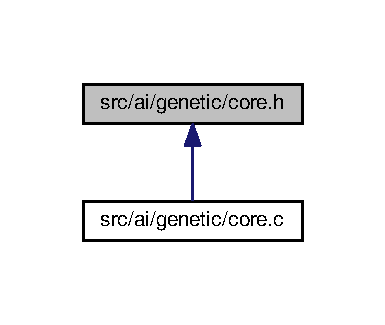
\includegraphics[width=185pt]{core_8h__dep__incl}
\end{center}
\end{figure}
\subsection*{Functions}
\begin{DoxyCompactItemize}
\item 
void \textbf{ genetic\+\_\+show\+\_\+stats} (\textbf{ State} $\ast$state)
\end{DoxyCompactItemize}


\subsection{Detailed Description}
Core of the genetic algorithm. 

\begin{DoxyAuthor}{Author}
S4\+Master\+Race 
\end{DoxyAuthor}
\begin{DoxyVersion}{Version}
2.\+0 
\end{DoxyVersion}


\subsection{Function Documentation}
\mbox{\label{core_8h_a471131fbd6fb873da1e9e9e34866f35b}} 
\index{core.\+h@{core.\+h}!genetic\+\_\+show\+\_\+stats@{genetic\+\_\+show\+\_\+stats}}
\index{genetic\+\_\+show\+\_\+stats@{genetic\+\_\+show\+\_\+stats}!core.\+h@{core.\+h}}
\subsubsection{genetic\+\_\+show\+\_\+stats()}
{\footnotesize\ttfamily void genetic\+\_\+show\+\_\+stats (\begin{DoxyParamCaption}\item[{\textbf{ State} $\ast$}]{state }\end{DoxyParamCaption})}


\section{src/ai/genetic/engine.c File Reference}
\label{engine_8c}\index{src/ai/genetic/engine.\+c@{src/ai/genetic/engine.\+c}}
{\ttfamily \#include \char`\"{}engine.\+h\char`\"{}}\newline
Include dependency graph for engine.\+c\+:
\nopagebreak
\begin{figure}[H]
\begin{center}
\leavevmode
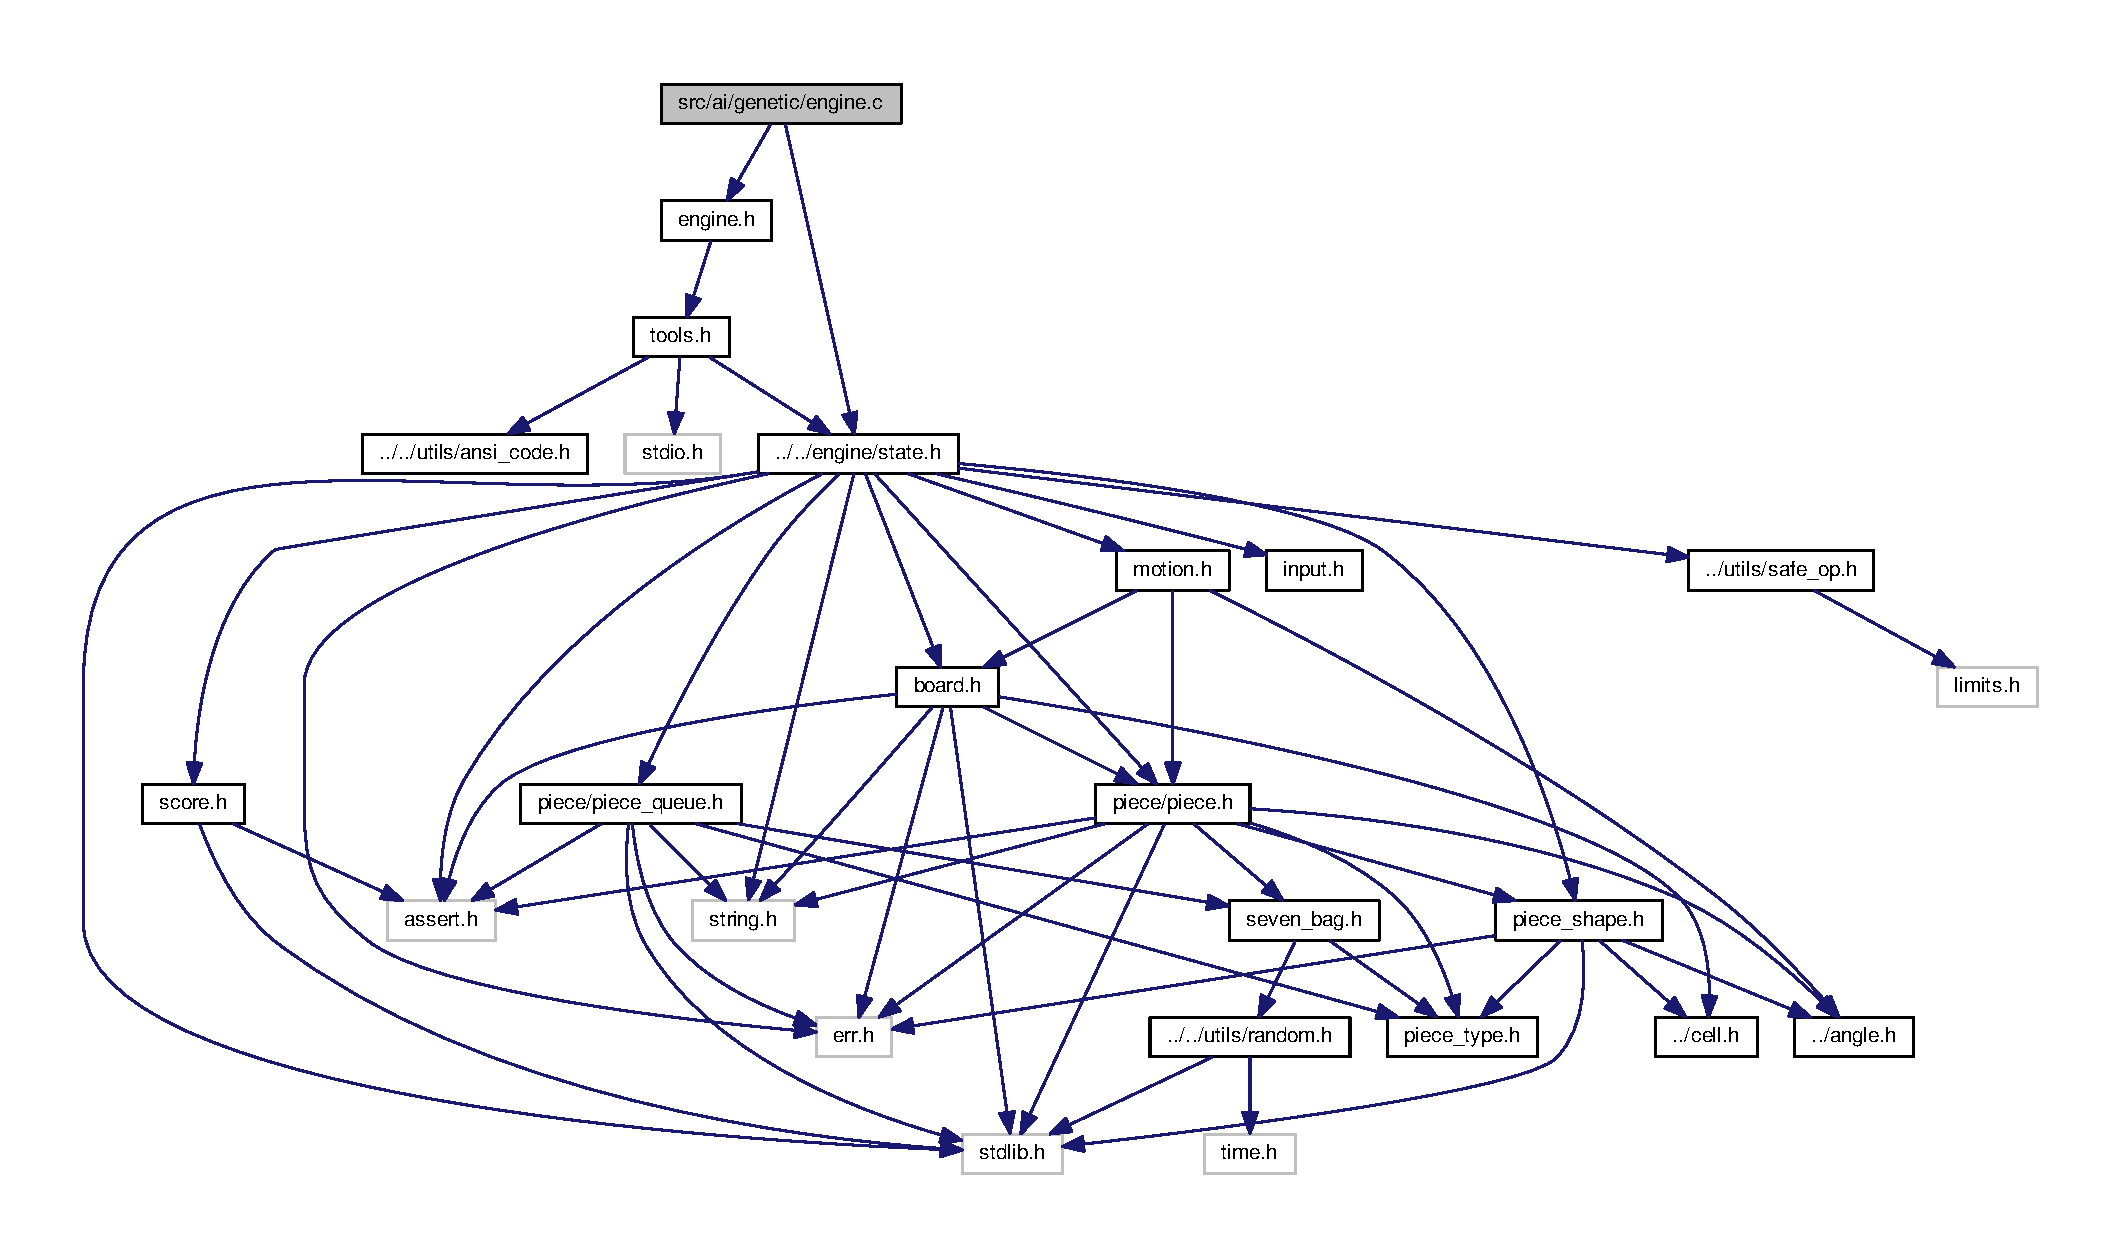
\includegraphics[width=350pt]{engine_8c__incl}
\end{center}
\end{figure}

\section{src/ai/genetic/engine.h File Reference}
\label{engine_8h}\index{src/ai/genetic/engine.\+h@{src/ai/genetic/engine.\+h}}
{\ttfamily \#include \char`\"{}tools.\+h\char`\"{}}\newline
Include dependency graph for engine.\+h\+:
\nopagebreak
\begin{figure}[H]
\begin{center}
\leavevmode
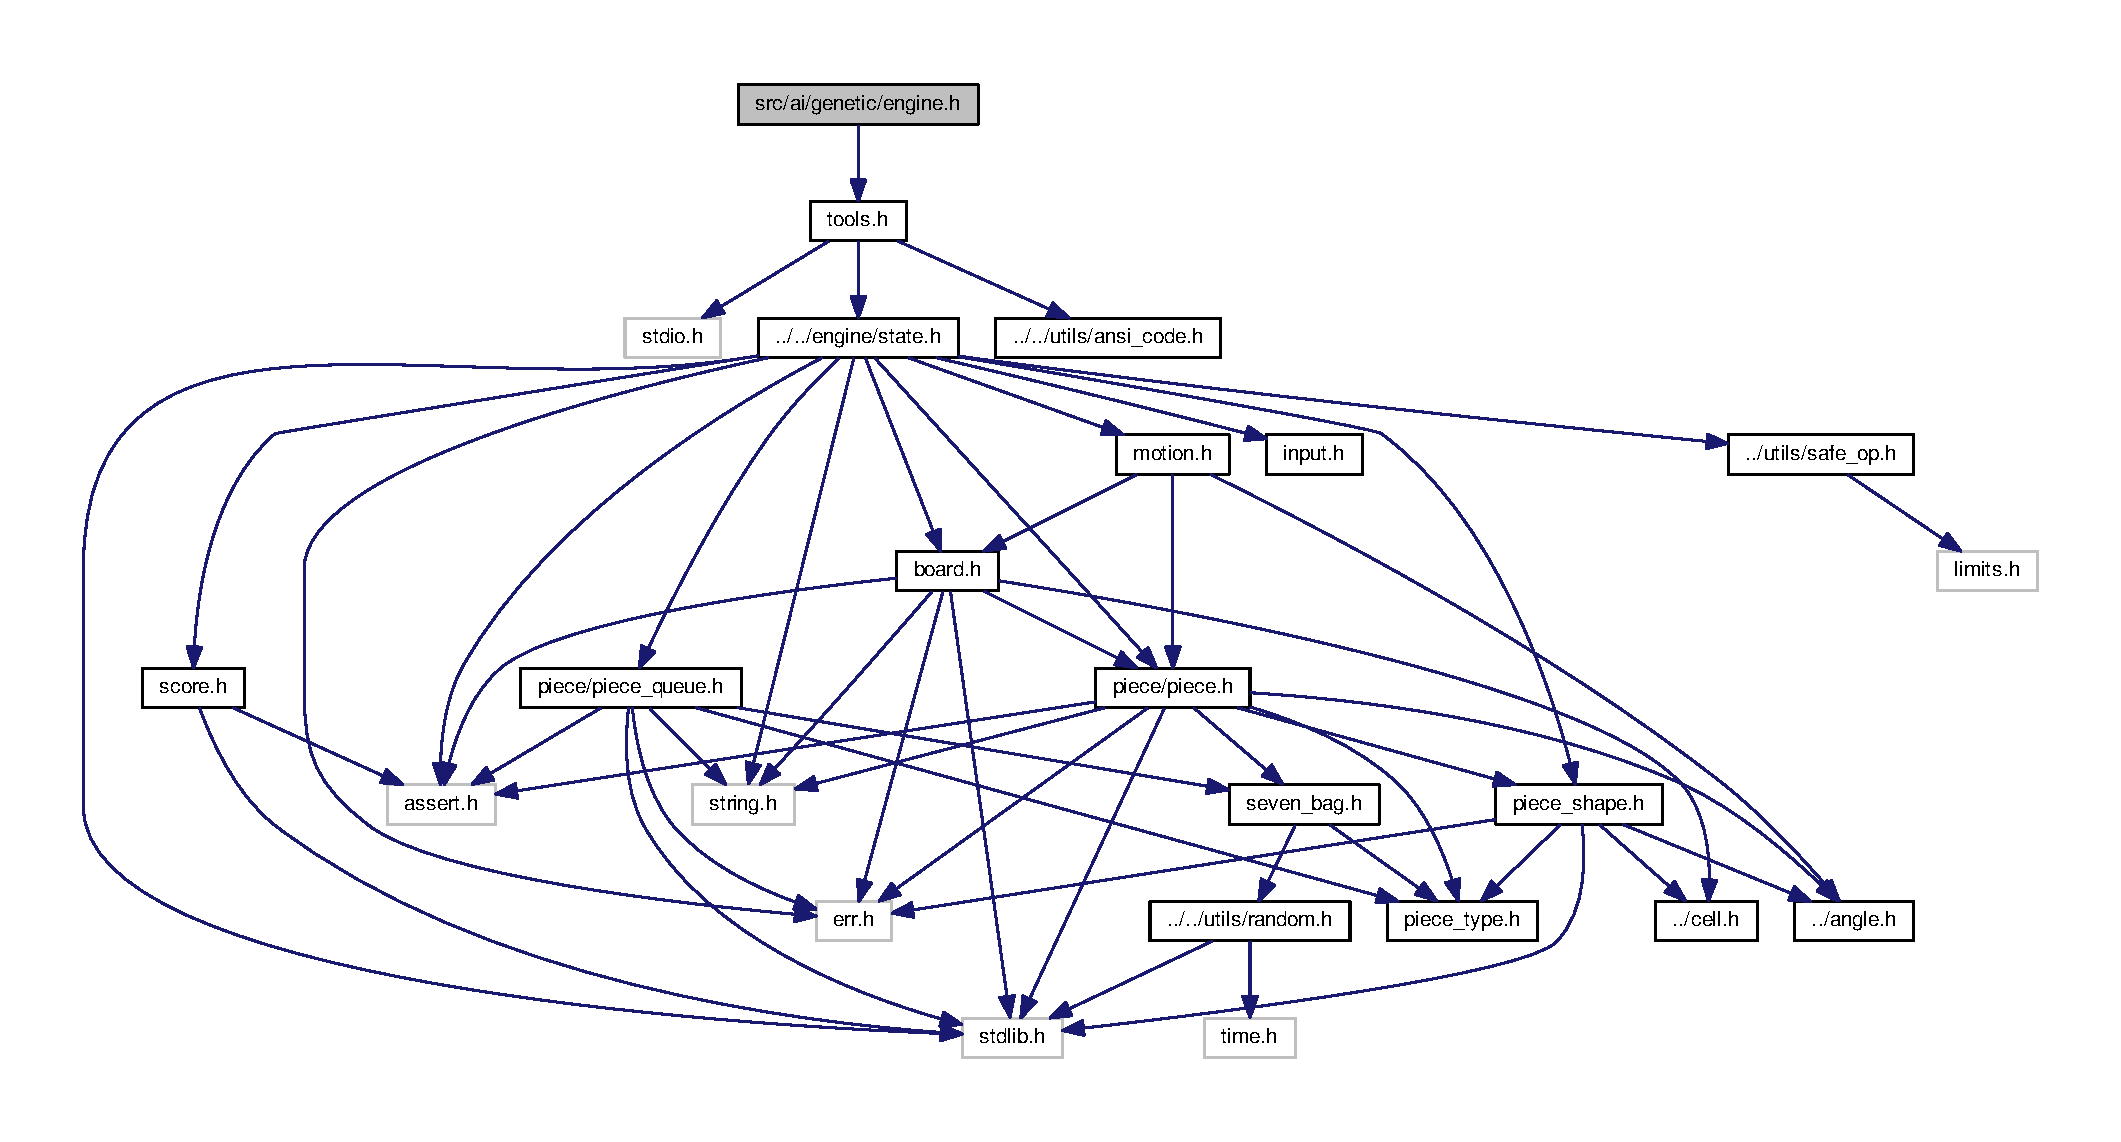
\includegraphics[width=350pt]{engine_8h__incl}
\end{center}
\end{figure}
This graph shows which files directly or indirectly include this file\+:
\nopagebreak
\begin{figure}[H]
\begin{center}
\leavevmode
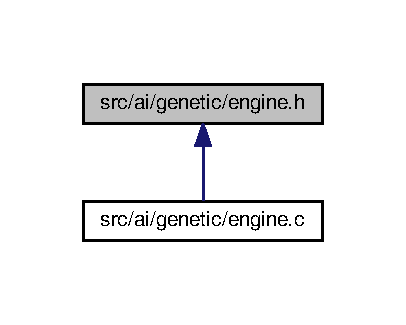
\includegraphics[width=195pt]{engine_8h__dep__incl}
\end{center}
\end{figure}
\subsection*{Data Structures}
\begin{DoxyCompactItemize}
\item 
struct \textbf{ ai\+\_\+coefs}
\end{DoxyCompactItemize}

\section{src/ai/genetic/tools.c File Reference}
\label{tools_8c}\index{src/ai/genetic/tools.\+c@{src/ai/genetic/tools.\+c}}


Tools for the genetic algorithm.  


{\ttfamily \#include \char`\"{}tools.\+h\char`\"{}}\newline
Include dependency graph for tools.\+c\+:
\nopagebreak
\begin{figure}[H]
\begin{center}
\leavevmode
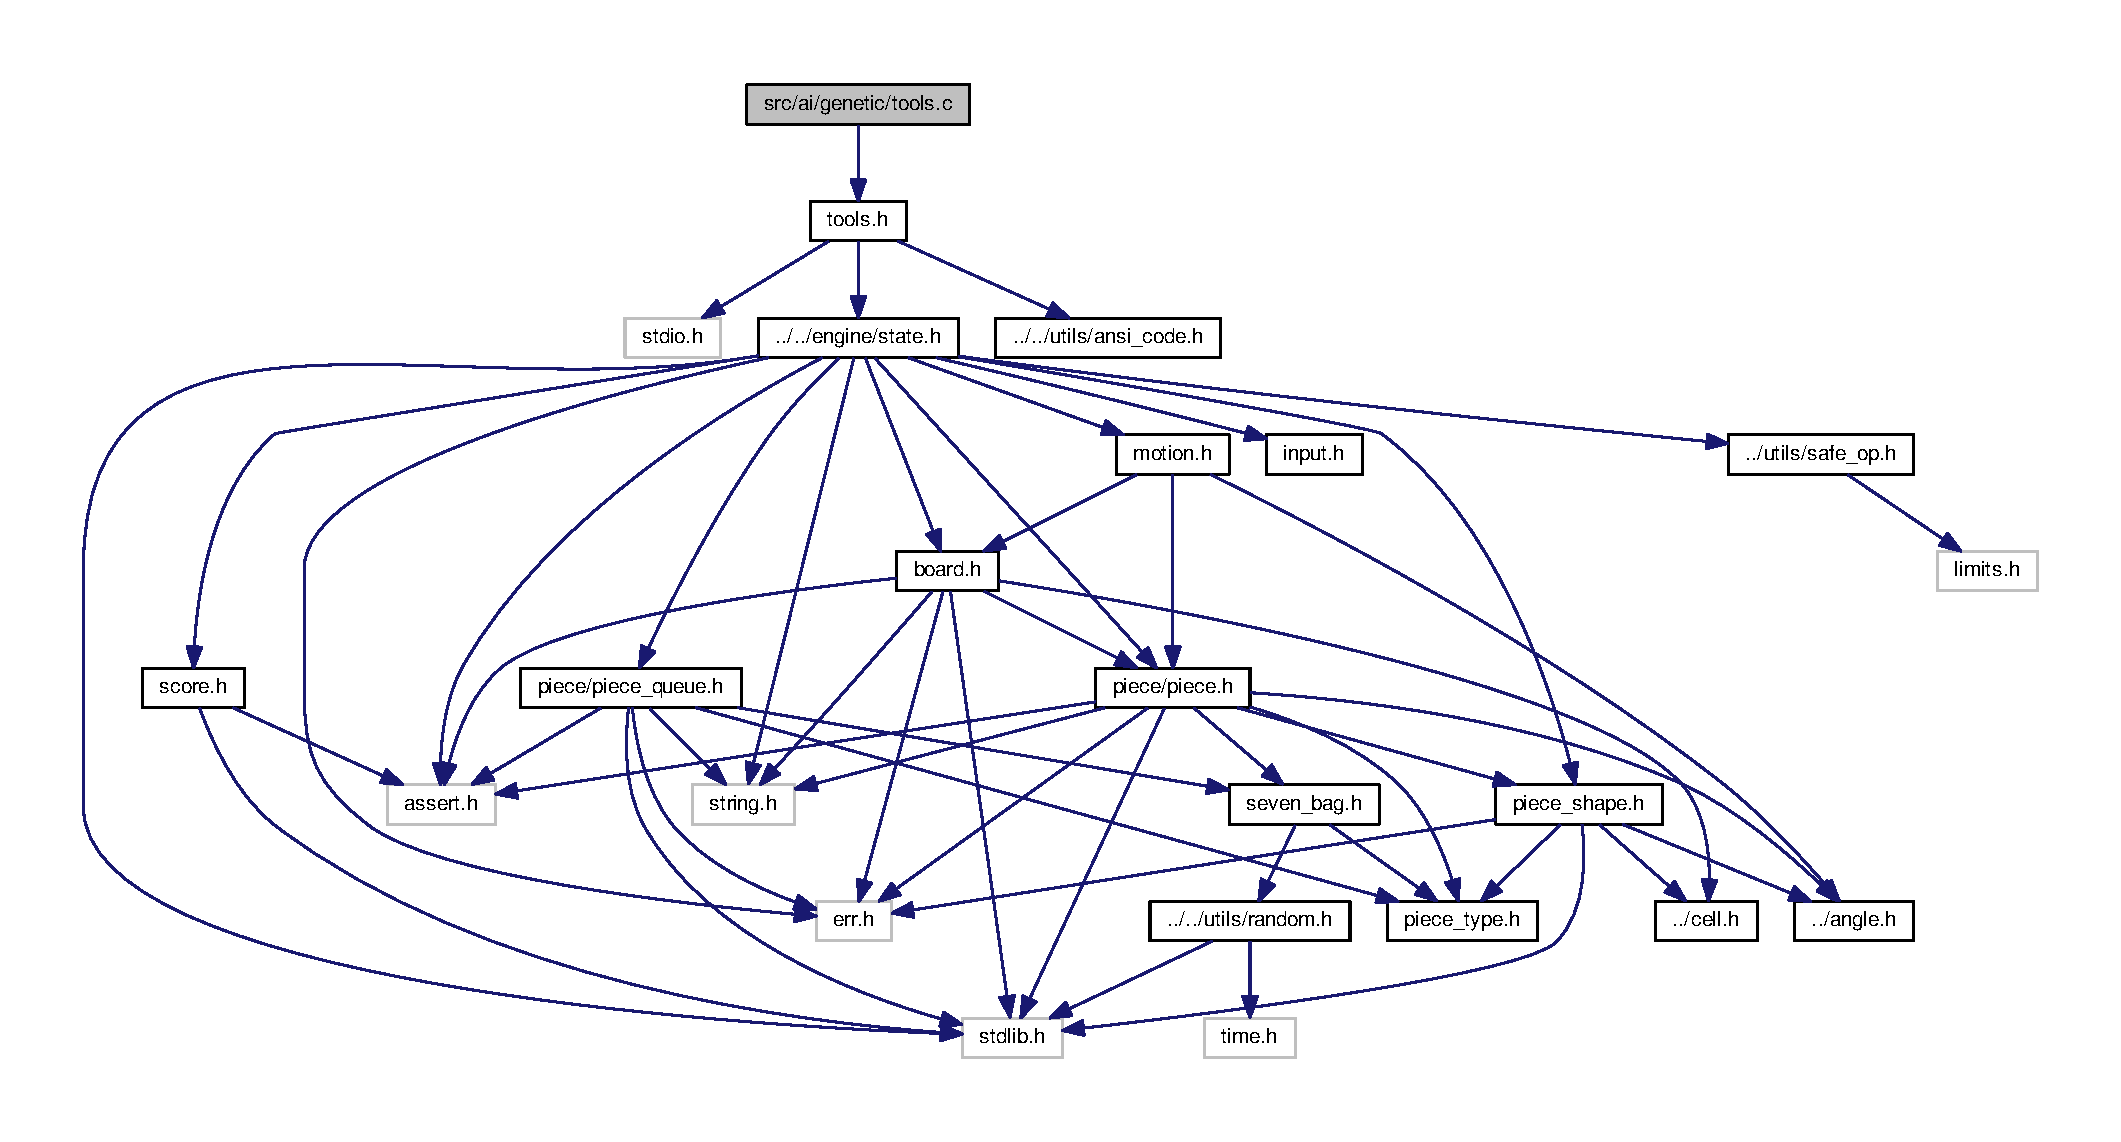
\includegraphics[width=350pt]{tools_8c__incl}
\end{center}
\end{figure}
\subsection*{Functions}
\begin{DoxyCompactItemize}
\item 
void \textbf{ board\+\_\+heights} (const \textbf{ Board} $\ast$brd, int $\ast$heights)
\item 
int \textbf{ board\+\_\+height} (const \textbf{ Board} $\ast$brd, int x)
\item 
int \textbf{ bumpiness} (const \textbf{ Board} $\ast$brd)
\item 
int \textbf{ aggregate\+\_\+height} (const \textbf{ Board} $\ast$brd)
\item 
int \textbf{ hole} (const \textbf{ Board} $\ast$brd, int x)
\item 
int \textbf{ holes} (const \textbf{ Board} $\ast$brd)
\item 
int \textbf{ clears} (const \textbf{ Board} $\ast$brd)
\item 
void \textbf{ show\+\_\+features} (const \textbf{ Board} $\ast$brd)
\end{DoxyCompactItemize}


\subsection{Detailed Description}
Tools for the genetic algorithm. 

\begin{DoxyAuthor}{Author}
S4\+Master\+Race 
\end{DoxyAuthor}
\begin{DoxyVersion}{Version}
2.\+0 
\end{DoxyVersion}


\subsection{Function Documentation}
\mbox{\label{tools_8c_ad841ef8c1553fc39aedf9ff99c4338c8}} 
\index{tools.\+c@{tools.\+c}!aggregate\+\_\+height@{aggregate\+\_\+height}}
\index{aggregate\+\_\+height@{aggregate\+\_\+height}!tools.\+c@{tools.\+c}}
\subsubsection{aggregate\+\_\+height()}
{\footnotesize\ttfamily int aggregate\+\_\+height (\begin{DoxyParamCaption}\item[{const \textbf{ Board} $\ast$}]{brd }\end{DoxyParamCaption})}

\mbox{\label{tools_8c_a91ae5afacda12393e4a93ca8c298832c}} 
\index{tools.\+c@{tools.\+c}!board\+\_\+height@{board\+\_\+height}}
\index{board\+\_\+height@{board\+\_\+height}!tools.\+c@{tools.\+c}}
\subsubsection{board\+\_\+height()}
{\footnotesize\ttfamily int board\+\_\+height (\begin{DoxyParamCaption}\item[{const \textbf{ Board} $\ast$}]{brd,  }\item[{int}]{x }\end{DoxyParamCaption})}

\mbox{\label{tools_8c_a0074ffa2b0873ffccfdbc813ccf02ba0}} 
\index{tools.\+c@{tools.\+c}!board\+\_\+heights@{board\+\_\+heights}}
\index{board\+\_\+heights@{board\+\_\+heights}!tools.\+c@{tools.\+c}}
\subsubsection{board\+\_\+heights()}
{\footnotesize\ttfamily void board\+\_\+heights (\begin{DoxyParamCaption}\item[{const \textbf{ Board} $\ast$}]{brd,  }\item[{int $\ast$}]{heights }\end{DoxyParamCaption})}

\mbox{\label{tools_8c_aa5a5f3a20ab3b8a9894c2826b02f5a70}} 
\index{tools.\+c@{tools.\+c}!bumpiness@{bumpiness}}
\index{bumpiness@{bumpiness}!tools.\+c@{tools.\+c}}
\subsubsection{bumpiness()}
{\footnotesize\ttfamily int bumpiness (\begin{DoxyParamCaption}\item[{const \textbf{ Board} $\ast$}]{brd }\end{DoxyParamCaption})}

\mbox{\label{tools_8c_a60fe37bb659ce363f8e7dc89e221bc3a}} 
\index{tools.\+c@{tools.\+c}!clears@{clears}}
\index{clears@{clears}!tools.\+c@{tools.\+c}}
\subsubsection{clears()}
{\footnotesize\ttfamily int clears (\begin{DoxyParamCaption}\item[{const \textbf{ Board} $\ast$}]{brd }\end{DoxyParamCaption})}

\mbox{\label{tools_8c_aa78f4d6d22d659aad248e39e379361db}} 
\index{tools.\+c@{tools.\+c}!hole@{hole}}
\index{hole@{hole}!tools.\+c@{tools.\+c}}
\subsubsection{hole()}
{\footnotesize\ttfamily int hole (\begin{DoxyParamCaption}\item[{const \textbf{ Board} $\ast$}]{brd,  }\item[{int}]{x }\end{DoxyParamCaption})}

\mbox{\label{tools_8c_af5aed4274764b48658e2572c7f5fcd8c}} 
\index{tools.\+c@{tools.\+c}!holes@{holes}}
\index{holes@{holes}!tools.\+c@{tools.\+c}}
\subsubsection{holes()}
{\footnotesize\ttfamily int holes (\begin{DoxyParamCaption}\item[{const \textbf{ Board} $\ast$}]{brd }\end{DoxyParamCaption})}

\mbox{\label{tools_8c_a453fbdbb55f005553eadfe4e955a6183}} 
\index{tools.\+c@{tools.\+c}!show\+\_\+features@{show\+\_\+features}}
\index{show\+\_\+features@{show\+\_\+features}!tools.\+c@{tools.\+c}}
\subsubsection{show\+\_\+features()}
{\footnotesize\ttfamily void show\+\_\+features (\begin{DoxyParamCaption}\item[{const \textbf{ Board} $\ast$}]{brd }\end{DoxyParamCaption})}


\section{src/ai/genetic/tools.h File Reference}
\label{tools_8h}\index{src/ai/genetic/tools.\+h@{src/ai/genetic/tools.\+h}}
{\ttfamily \#include \char`\"{}../../core/board.\+h\char`\"{}}\newline
{\ttfamily \#include \char`\"{}../../core/game\+\_\+state.\+h\char`\"{}}\newline
{\ttfamily \#include \char`\"{}../../core/motion.\+h\char`\"{}}\newline
{\ttfamily \#include \char`\"{}../../core/piece.\+h\char`\"{}}\newline
Include dependency graph for tools.\+h\+:
\nopagebreak
\begin{figure}[H]
\begin{center}
\leavevmode
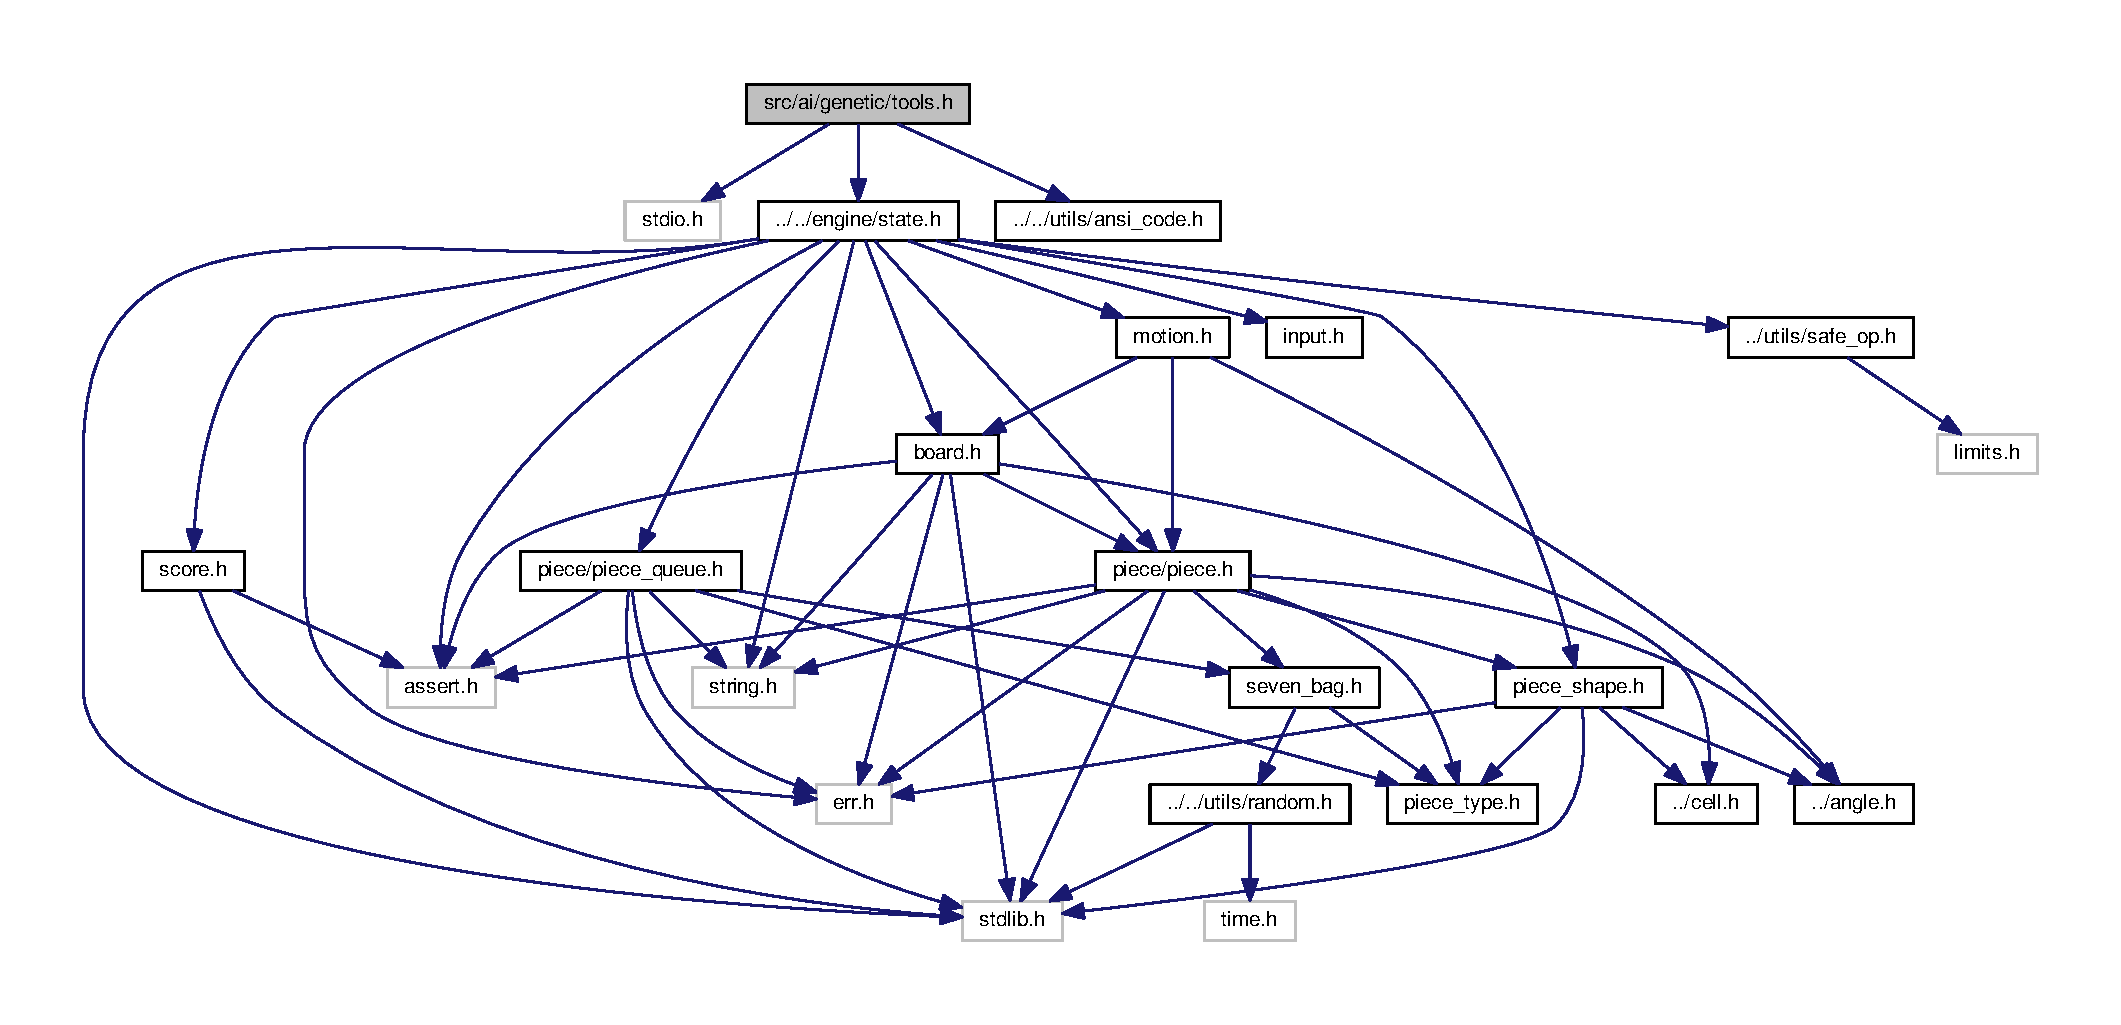
\includegraphics[width=350pt]{tools_8h__incl}
\end{center}
\end{figure}
This graph shows which files directly or indirectly include this file\+:
\nopagebreak
\begin{figure}[H]
\begin{center}
\leavevmode
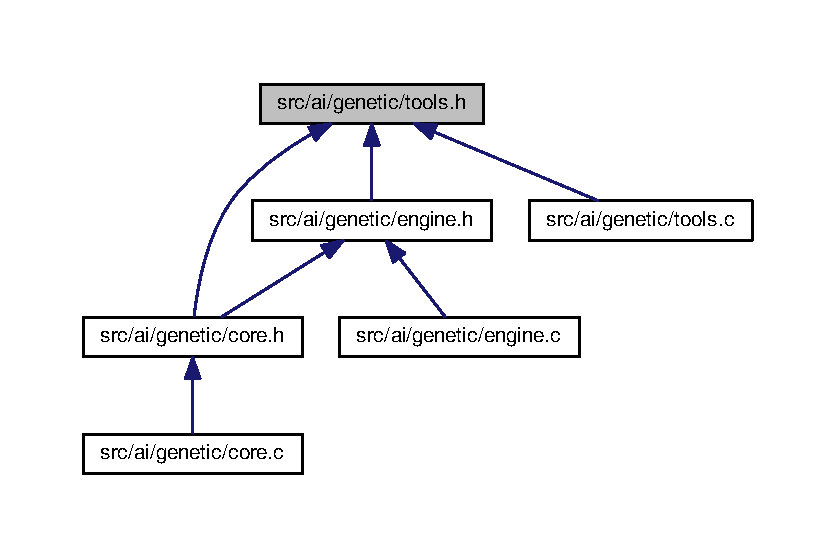
\includegraphics[width=320pt]{tools_8h__dep__incl}
\end{center}
\end{figure}
\subsection*{Macros}
\begin{DoxyCompactItemize}
\item 
\#define \textbf{ A\+BS}(X)~(((X) $<$ 0) ? (-\/1 $\ast$ (X)) \+: (X))
\end{DoxyCompactItemize}
\subsection*{Functions}
\begin{DoxyCompactItemize}
\item 
size\+\_\+t \textbf{ board\+\_\+height} (const struct \textbf{ board} $\ast$brd, size\+\_\+t x)
\item 
void \textbf{ board\+\_\+heights} (const struct \textbf{ board} $\ast$brd, size\+\_\+t $\ast$heights)
\item 
size\+\_\+t \textbf{ bumpiness} (const struct \textbf{ board} $\ast$brd)
\item 
size\+\_\+t \textbf{ aggregate\+\_\+height} (const struct \textbf{ board} $\ast$brd)
\item 
size\+\_\+t \textbf{ hole} (const struct \textbf{ board} $\ast$brd, size\+\_\+t x)
\item 
size\+\_\+t \textbf{ holes} (const struct \textbf{ board} $\ast$brd)
\item 
size\+\_\+t \textbf{ coalescent\+\_\+clears} (const struct \textbf{ board} $\ast$brd)
\item 
void \textbf{ make\+\_\+line} (struct \textbf{ board} $\ast$brd, size\+\_\+t y)
\item 
size\+\_\+t \textbf{ clears} (const struct \textbf{ board} $\ast$brd)
\end{DoxyCompactItemize}


\subsection{Macro Definition Documentation}
\mbox{\label{tools_8h_adefab4344518e9d35a80d87c20c0fa48}} 
\index{tools.\+h@{tools.\+h}!A\+BS@{A\+BS}}
\index{A\+BS@{A\+BS}!tools.\+h@{tools.\+h}}
\subsubsection{A\+BS}
{\footnotesize\ttfamily \#define A\+BS(\begin{DoxyParamCaption}\item[{}]{X }\end{DoxyParamCaption})~(((X) $<$ 0) ? (-\/1 $\ast$ (X)) \+: (X))}



\subsection{Function Documentation}
\mbox{\label{tools_8h_af641e6b38f455ac3f9f1a5f49d3bc787}} 
\index{tools.\+h@{tools.\+h}!aggregate\+\_\+height@{aggregate\+\_\+height}}
\index{aggregate\+\_\+height@{aggregate\+\_\+height}!tools.\+h@{tools.\+h}}
\subsubsection{aggregate\+\_\+height()}
{\footnotesize\ttfamily size\+\_\+t aggregate\+\_\+height (\begin{DoxyParamCaption}\item[{const struct \textbf{ board} $\ast$}]{brd }\end{DoxyParamCaption})\hspace{0.3cm}{\ttfamily [inline]}}

\mbox{\label{tools_8h_a4ca7e6505b351ba190d31948268ff2cb}} 
\index{tools.\+h@{tools.\+h}!board\+\_\+height@{board\+\_\+height}}
\index{board\+\_\+height@{board\+\_\+height}!tools.\+h@{tools.\+h}}
\subsubsection{board\+\_\+height()}
{\footnotesize\ttfamily size\+\_\+t board\+\_\+height (\begin{DoxyParamCaption}\item[{const struct \textbf{ board} $\ast$}]{brd,  }\item[{size\+\_\+t}]{x }\end{DoxyParamCaption})\hspace{0.3cm}{\ttfamily [inline]}}

\mbox{\label{tools_8h_ab2be749cc3ff926d84d4d19b40db0c5f}} 
\index{tools.\+h@{tools.\+h}!board\+\_\+heights@{board\+\_\+heights}}
\index{board\+\_\+heights@{board\+\_\+heights}!tools.\+h@{tools.\+h}}
\subsubsection{board\+\_\+heights()}
{\footnotesize\ttfamily void board\+\_\+heights (\begin{DoxyParamCaption}\item[{const struct \textbf{ board} $\ast$}]{brd,  }\item[{size\+\_\+t $\ast$}]{heights }\end{DoxyParamCaption})\hspace{0.3cm}{\ttfamily [inline]}}

\mbox{\label{tools_8h_a32300283b4df94743b9dae9d7bdaf119}} 
\index{tools.\+h@{tools.\+h}!bumpiness@{bumpiness}}
\index{bumpiness@{bumpiness}!tools.\+h@{tools.\+h}}
\subsubsection{bumpiness()}
{\footnotesize\ttfamily size\+\_\+t bumpiness (\begin{DoxyParamCaption}\item[{const struct \textbf{ board} $\ast$}]{brd }\end{DoxyParamCaption})\hspace{0.3cm}{\ttfamily [inline]}}

\mbox{\label{tools_8h_afd326c0778c693b0752754323b425bd2}} 
\index{tools.\+h@{tools.\+h}!clears@{clears}}
\index{clears@{clears}!tools.\+h@{tools.\+h}}
\subsubsection{clears()}
{\footnotesize\ttfamily size\+\_\+t clears (\begin{DoxyParamCaption}\item[{const struct \textbf{ board} $\ast$}]{brd }\end{DoxyParamCaption})\hspace{0.3cm}{\ttfamily [inline]}}

\mbox{\label{tools_8h_ac556c43db39f31aabe6297e22966a9f3}} 
\index{tools.\+h@{tools.\+h}!coalescent\+\_\+clears@{coalescent\+\_\+clears}}
\index{coalescent\+\_\+clears@{coalescent\+\_\+clears}!tools.\+h@{tools.\+h}}
\subsubsection{coalescent\+\_\+clears()}
{\footnotesize\ttfamily size\+\_\+t coalescent\+\_\+clears (\begin{DoxyParamCaption}\item[{const struct \textbf{ board} $\ast$}]{brd }\end{DoxyParamCaption})\hspace{0.3cm}{\ttfamily [inline]}}

\mbox{\label{tools_8h_a1415ca3c57c0a6fdb689276670d75c90}} 
\index{tools.\+h@{tools.\+h}!hole@{hole}}
\index{hole@{hole}!tools.\+h@{tools.\+h}}
\subsubsection{hole()}
{\footnotesize\ttfamily size\+\_\+t hole (\begin{DoxyParamCaption}\item[{const struct \textbf{ board} $\ast$}]{brd,  }\item[{size\+\_\+t}]{x }\end{DoxyParamCaption})\hspace{0.3cm}{\ttfamily [inline]}}

\mbox{\label{tools_8h_a0febcc8c076fd7843176561167fabac1}} 
\index{tools.\+h@{tools.\+h}!holes@{holes}}
\index{holes@{holes}!tools.\+h@{tools.\+h}}
\subsubsection{holes()}
{\footnotesize\ttfamily size\+\_\+t holes (\begin{DoxyParamCaption}\item[{const struct \textbf{ board} $\ast$}]{brd }\end{DoxyParamCaption})\hspace{0.3cm}{\ttfamily [inline]}}

\mbox{\label{tools_8h_a97d0b3536ca1b715182ae405fd4fe643}} 
\index{tools.\+h@{tools.\+h}!make\+\_\+line@{make\+\_\+line}}
\index{make\+\_\+line@{make\+\_\+line}!tools.\+h@{tools.\+h}}
\subsubsection{make\+\_\+line()}
{\footnotesize\ttfamily void make\+\_\+line (\begin{DoxyParamCaption}\item[{struct \textbf{ board} $\ast$}]{brd,  }\item[{size\+\_\+t}]{y }\end{DoxyParamCaption})\hspace{0.3cm}{\ttfamily [inline]}}


\section{src/debug/debug.h File Reference}
\label{debug_8h}\index{src/debug/debug.\+h@{src/debug/debug.\+h}}


Debug.  


{\ttfamily \#include \char`\"{}../utils/ansi\+\_\+code.\+h\char`\"{}}\newline
Include dependency graph for debug.\+h\+:
\nopagebreak
\begin{figure}[H]
\begin{center}
\leavevmode
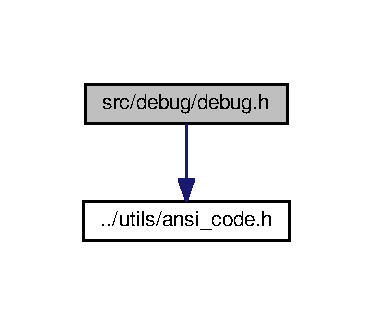
\includegraphics[width=179pt]{debug_8h__incl}
\end{center}
\end{figure}
This graph shows which files directly or indirectly include this file\+:
\nopagebreak
\begin{figure}[H]
\begin{center}
\leavevmode
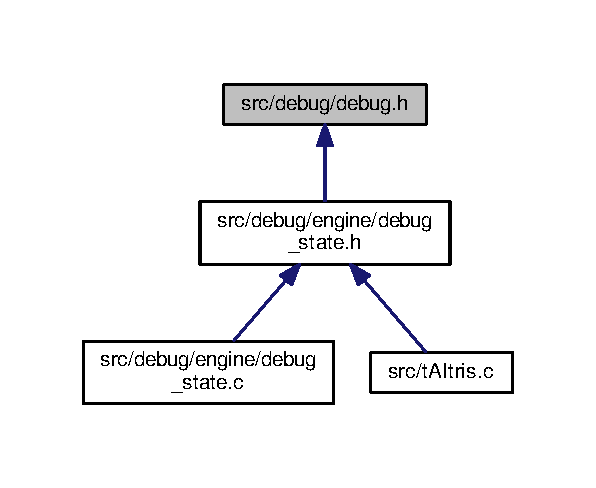
\includegraphics[width=286pt]{debug_8h__dep__incl}
\end{center}
\end{figure}
\subsection*{Macros}
\begin{DoxyCompactItemize}
\item 
\#define \textbf{ D\+E\+B\+U\+G\+\_\+\+T\+AG}(\+\_\+name\+\_\+,  \+\_\+color\+\_\+)
\end{DoxyCompactItemize}


\subsection{Detailed Description}
Debug. 

\begin{DoxyAuthor}{Author}
S4\+Master\+Race 
\end{DoxyAuthor}
\begin{DoxyVersion}{Version}
2.\+0 
\end{DoxyVersion}


\subsection{Macro Definition Documentation}
\mbox{\label{debug_8h_a78999266903dfc706993a8a91aba6991}} 
\index{debug.\+h@{debug.\+h}!D\+E\+B\+U\+G\+\_\+\+T\+AG@{D\+E\+B\+U\+G\+\_\+\+T\+AG}}
\index{D\+E\+B\+U\+G\+\_\+\+T\+AG@{D\+E\+B\+U\+G\+\_\+\+T\+AG}!debug.\+h@{debug.\+h}}
\subsubsection{D\+E\+B\+U\+G\+\_\+\+T\+AG}
{\footnotesize\ttfamily \#define D\+E\+B\+U\+G\+\_\+\+T\+AG(\begin{DoxyParamCaption}\item[{}]{\+\_\+name\+\_\+,  }\item[{}]{\+\_\+color\+\_\+ }\end{DoxyParamCaption})}

{\bfseries Value\+:}
\begin{DoxyCode}
ANSI_RESET \(\backslash\)
  \textcolor{stringliteral}{"["} ANSI_FG_CYAN \textcolor{stringliteral}{"Debug"} ANSI_RESET \textcolor{stringliteral}{"]"} \(\backslash\)
  \textcolor{stringliteral}{"("} \_color\_ \_name\_ ANSI_RESET \textcolor{stringliteral}{") "}
\end{DoxyCode}

\section{src/debug/engine/debug\+\_\+state.c File Reference}
\label{debug__state_8c}\index{src/debug/engine/debug\+\_\+state.\+c@{src/debug/engine/debug\+\_\+state.\+c}}


Debug state.  


{\ttfamily \#include \char`\"{}debug\+\_\+state.\+h\char`\"{}}\newline
Include dependency graph for debug\+\_\+state.\+c\+:
\nopagebreak
\begin{figure}[H]
\begin{center}
\leavevmode
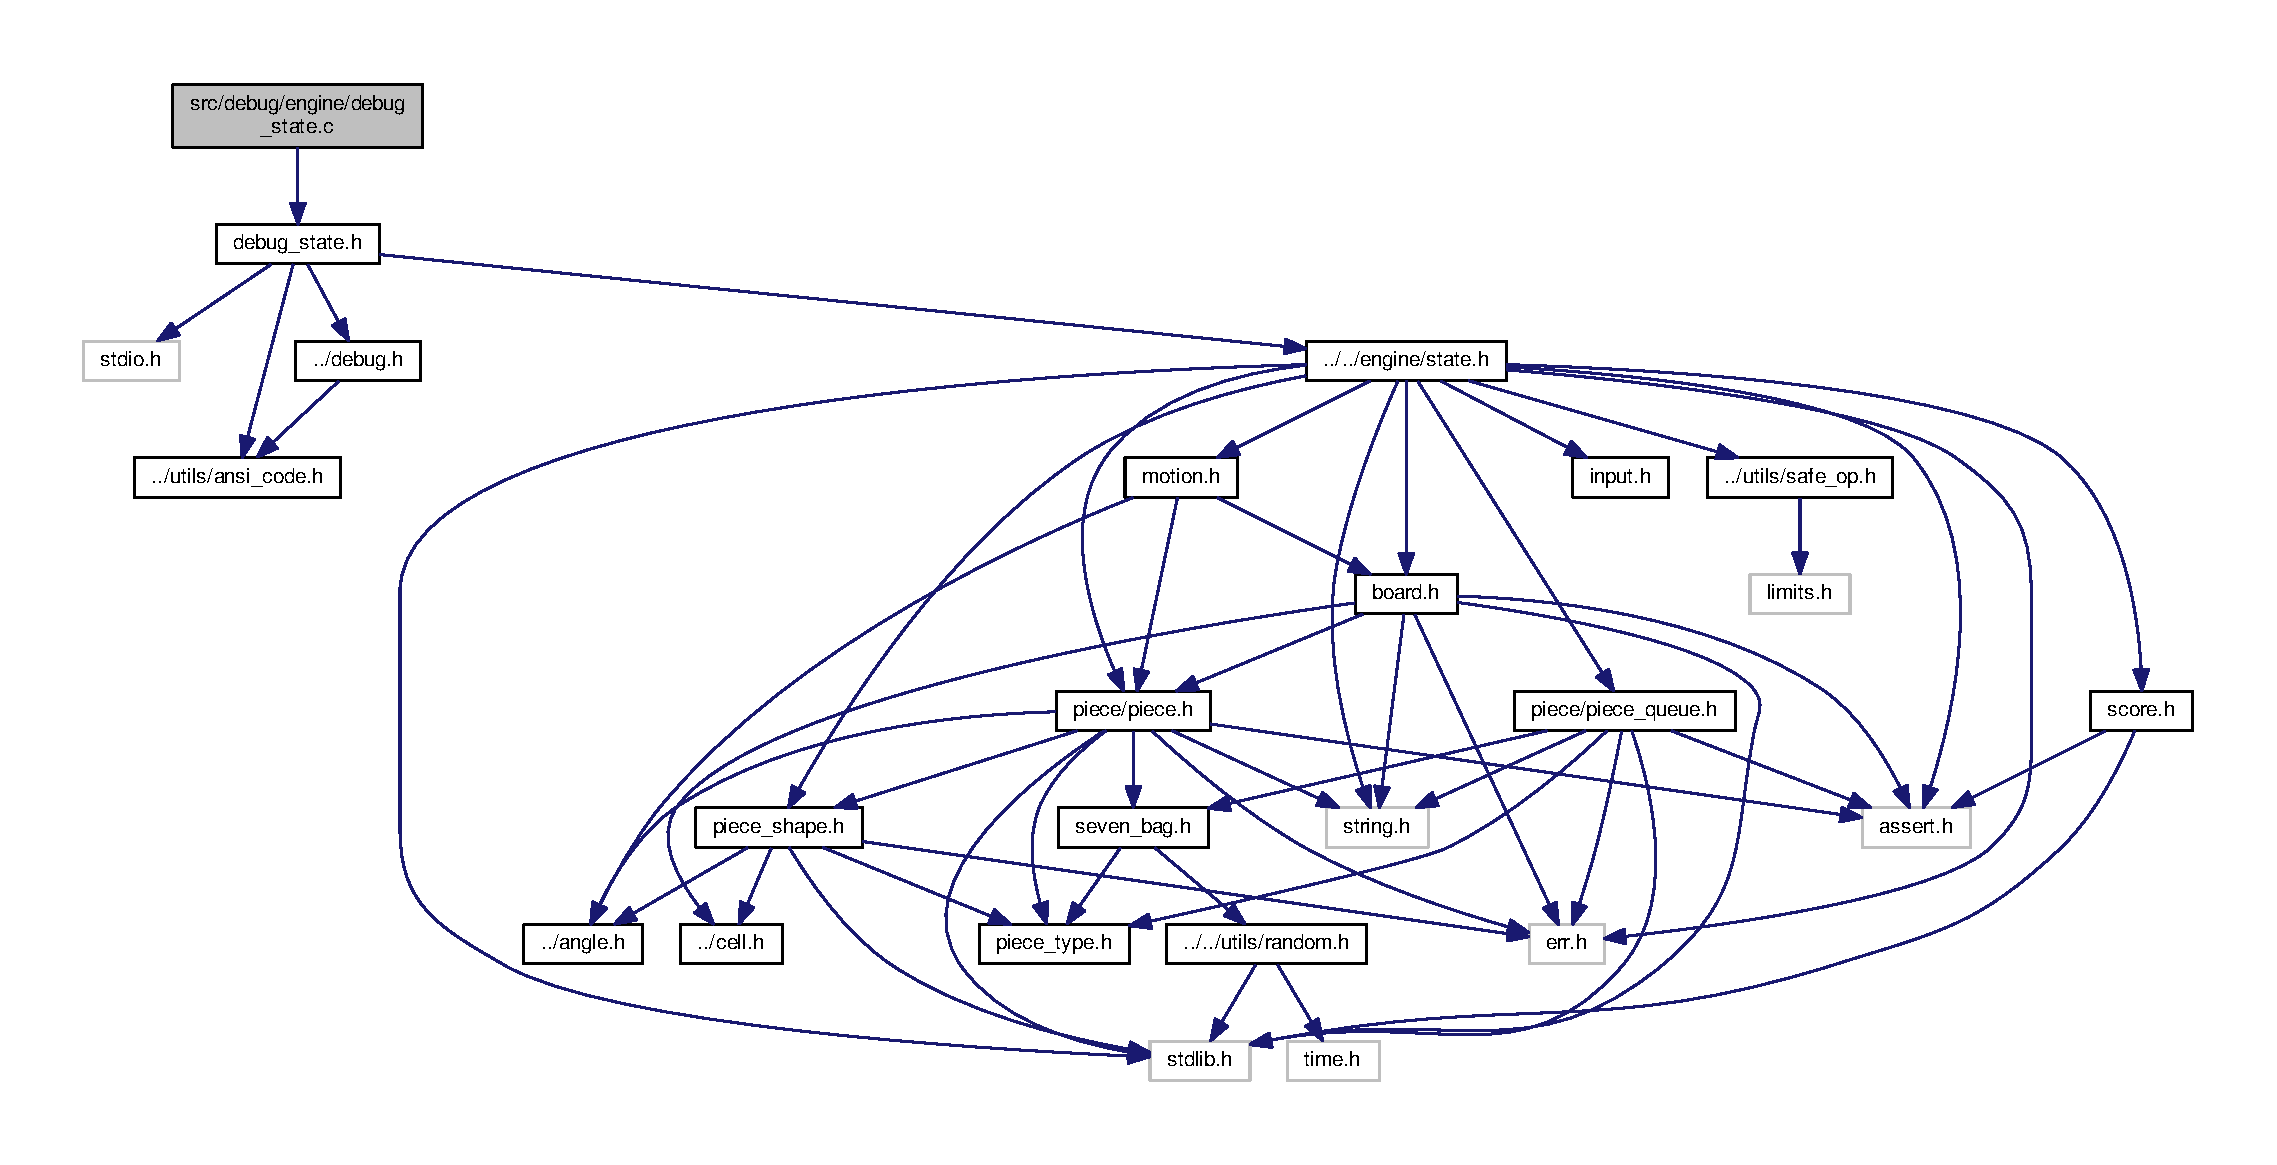
\includegraphics[width=350pt]{debug__state_8c__incl}
\end{center}
\end{figure}
\subsection*{Functions}
\begin{DoxyCompactItemize}
\item 
void \textbf{ debug\+\_\+state\+\_\+print\+\_\+line\+\_\+number} (const \textbf{ Board} $\ast$brd, int y)
\item 
void \textbf{ debug\+\_\+state\+\_\+print\+\_\+cell} (\textbf{ Cell} c)
\item 
void \textbf{ debug\+\_\+state\+\_\+print\+\_\+infos} (const \textbf{ State} $\ast$state, int y)
\item 
void \textbf{ debug\+\_\+state\+\_\+print\+\_\+next\+\_\+piece} (const \textbf{ Piece} $\ast$pc, int y)
\item 
void \textbf{ debug\+\_\+state\+\_\+print} (const \textbf{ State} $\ast$state)
\end{DoxyCompactItemize}


\subsection{Detailed Description}
Debug state. 

\begin{DoxyAuthor}{Author}
S4\+Master\+Race 
\end{DoxyAuthor}
\begin{DoxyVersion}{Version}
2.\+0 
\end{DoxyVersion}


\subsection{Function Documentation}
\mbox{\label{debug__state_8c_a9c0699f48870100dee7ceaa45763dd16}} 
\index{debug\+\_\+state.\+c@{debug\+\_\+state.\+c}!debug\+\_\+state\+\_\+print@{debug\+\_\+state\+\_\+print}}
\index{debug\+\_\+state\+\_\+print@{debug\+\_\+state\+\_\+print}!debug\+\_\+state.\+c@{debug\+\_\+state.\+c}}
\subsubsection{debug\+\_\+state\+\_\+print()}
{\footnotesize\ttfamily void debug\+\_\+state\+\_\+print (\begin{DoxyParamCaption}\item[{const \textbf{ State} $\ast$}]{state }\end{DoxyParamCaption})}

\mbox{\label{debug__state_8c_a57bffc683e10d64829dfaee65aa44c99}} 
\index{debug\+\_\+state.\+c@{debug\+\_\+state.\+c}!debug\+\_\+state\+\_\+print\+\_\+cell@{debug\+\_\+state\+\_\+print\+\_\+cell}}
\index{debug\+\_\+state\+\_\+print\+\_\+cell@{debug\+\_\+state\+\_\+print\+\_\+cell}!debug\+\_\+state.\+c@{debug\+\_\+state.\+c}}
\subsubsection{debug\+\_\+state\+\_\+print\+\_\+cell()}
{\footnotesize\ttfamily void debug\+\_\+state\+\_\+print\+\_\+cell (\begin{DoxyParamCaption}\item[{\textbf{ Cell}}]{c }\end{DoxyParamCaption})}

\mbox{\label{debug__state_8c_aa72d3737296f3a5b97a6589dc5cd8a92}} 
\index{debug\+\_\+state.\+c@{debug\+\_\+state.\+c}!debug\+\_\+state\+\_\+print\+\_\+infos@{debug\+\_\+state\+\_\+print\+\_\+infos}}
\index{debug\+\_\+state\+\_\+print\+\_\+infos@{debug\+\_\+state\+\_\+print\+\_\+infos}!debug\+\_\+state.\+c@{debug\+\_\+state.\+c}}
\subsubsection{debug\+\_\+state\+\_\+print\+\_\+infos()}
{\footnotesize\ttfamily void debug\+\_\+state\+\_\+print\+\_\+infos (\begin{DoxyParamCaption}\item[{const \textbf{ State} $\ast$}]{state,  }\item[{int}]{y }\end{DoxyParamCaption})}

\mbox{\label{debug__state_8c_a068cc3486e3c89355ca784fdb55194b4}} 
\index{debug\+\_\+state.\+c@{debug\+\_\+state.\+c}!debug\+\_\+state\+\_\+print\+\_\+line\+\_\+number@{debug\+\_\+state\+\_\+print\+\_\+line\+\_\+number}}
\index{debug\+\_\+state\+\_\+print\+\_\+line\+\_\+number@{debug\+\_\+state\+\_\+print\+\_\+line\+\_\+number}!debug\+\_\+state.\+c@{debug\+\_\+state.\+c}}
\subsubsection{debug\+\_\+state\+\_\+print\+\_\+line\+\_\+number()}
{\footnotesize\ttfamily void debug\+\_\+state\+\_\+print\+\_\+line\+\_\+number (\begin{DoxyParamCaption}\item[{const \textbf{ Board} $\ast$}]{brd,  }\item[{int}]{y }\end{DoxyParamCaption})}

\mbox{\label{debug__state_8c_ad288c47f98f24b9d84b889182a207256}} 
\index{debug\+\_\+state.\+c@{debug\+\_\+state.\+c}!debug\+\_\+state\+\_\+print\+\_\+next\+\_\+piece@{debug\+\_\+state\+\_\+print\+\_\+next\+\_\+piece}}
\index{debug\+\_\+state\+\_\+print\+\_\+next\+\_\+piece@{debug\+\_\+state\+\_\+print\+\_\+next\+\_\+piece}!debug\+\_\+state.\+c@{debug\+\_\+state.\+c}}
\subsubsection{debug\+\_\+state\+\_\+print\+\_\+next\+\_\+piece()}
{\footnotesize\ttfamily void debug\+\_\+state\+\_\+print\+\_\+next\+\_\+piece (\begin{DoxyParamCaption}\item[{const \textbf{ Piece} $\ast$}]{pc,  }\item[{int}]{y }\end{DoxyParamCaption})}


\section{src/debug/engine/debug\+\_\+state.h File Reference}
\label{debug__state_8h}\index{src/debug/engine/debug\+\_\+state.\+h@{src/debug/engine/debug\+\_\+state.\+h}}


Debug state.  


{\ttfamily \#include $<$stdio.\+h$>$}\newline
{\ttfamily \#include \char`\"{}../debug.\+h\char`\"{}}\newline
{\ttfamily \#include \char`\"{}../../engine/state.\+h\char`\"{}}\newline
{\ttfamily \#include \char`\"{}../../utils/ansi\+\_\+code.\+h\char`\"{}}\newline
Include dependency graph for debug\+\_\+state.\+h\+:
\nopagebreak
\begin{figure}[H]
\begin{center}
\leavevmode
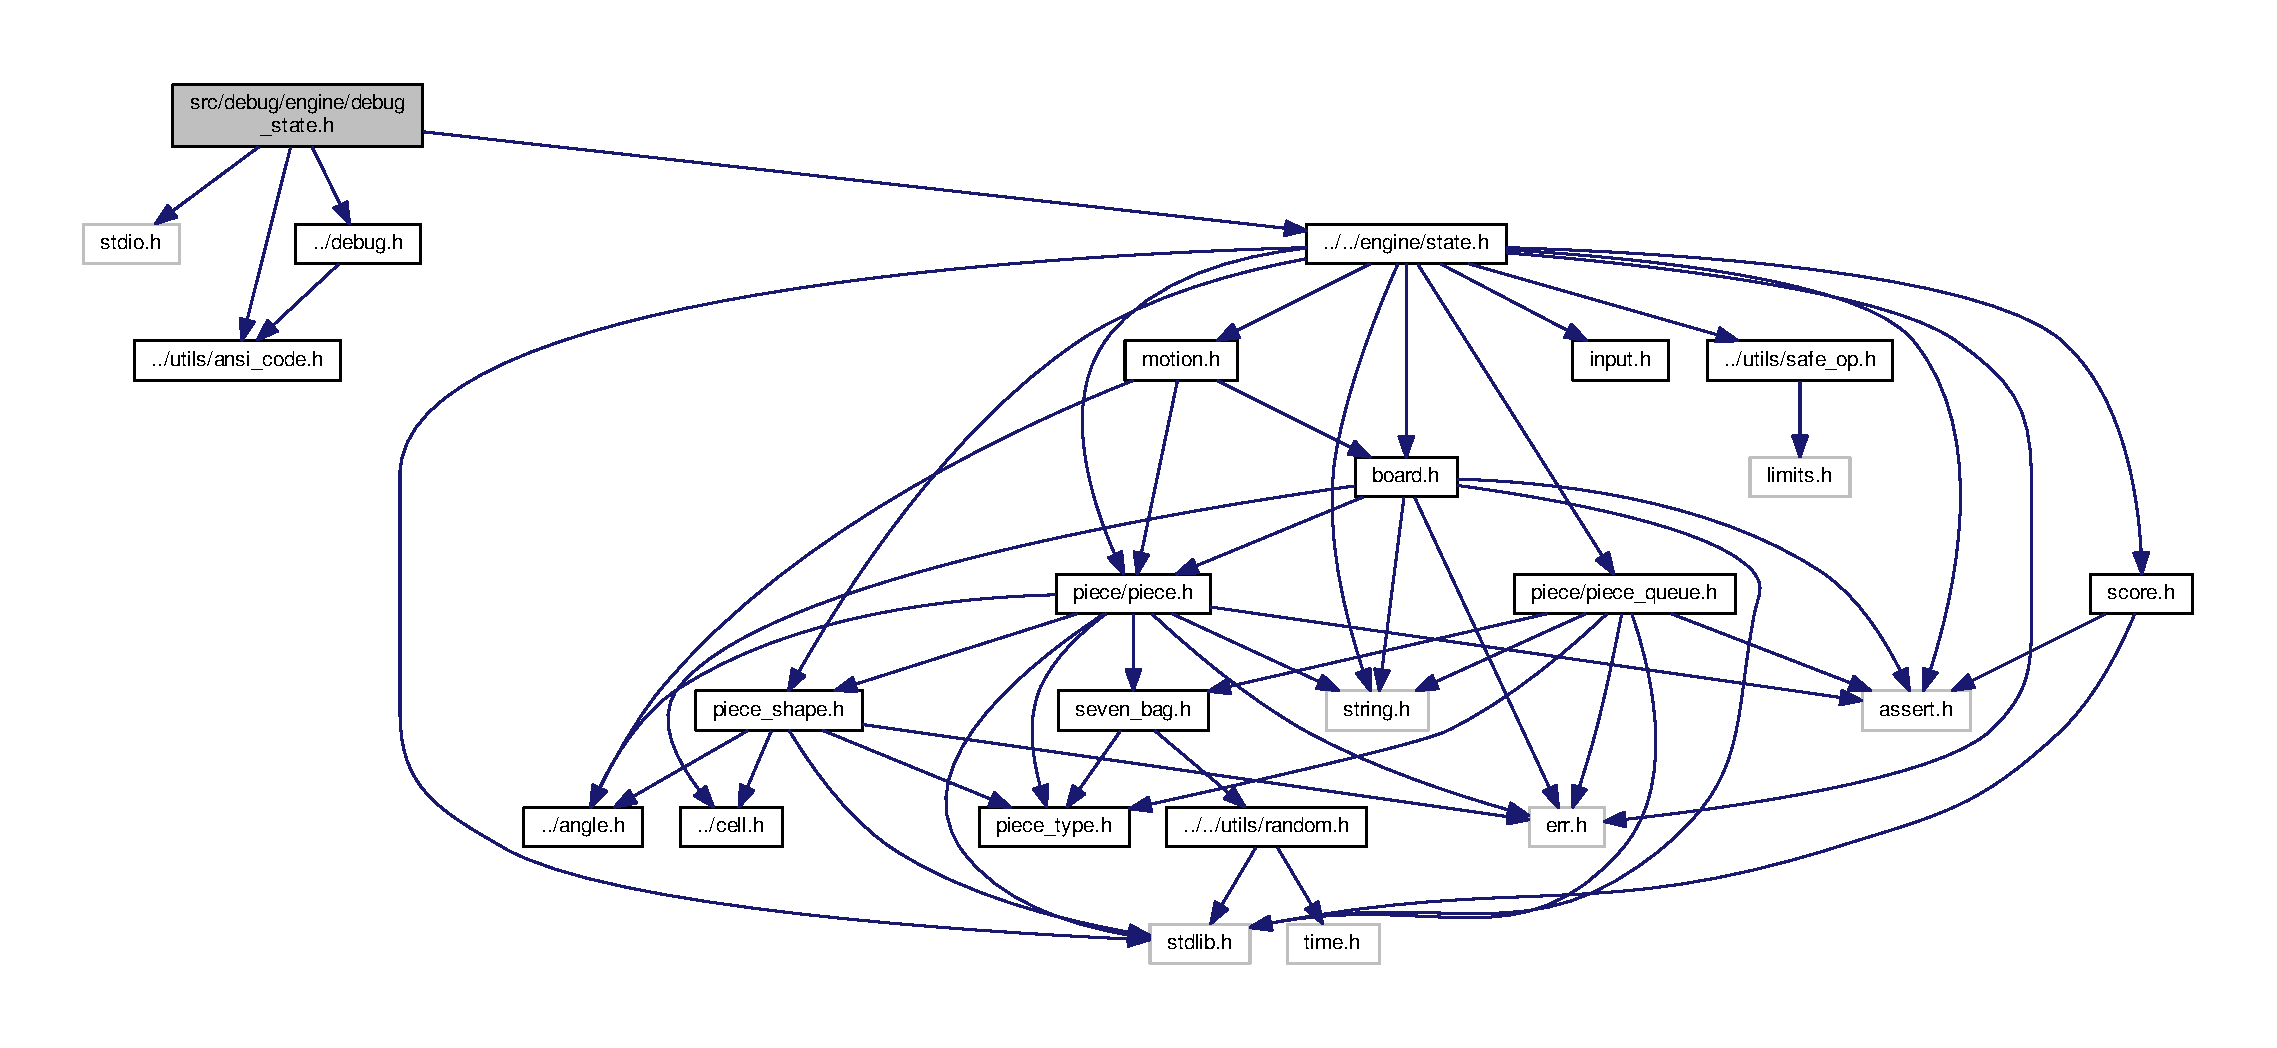
\includegraphics[width=350pt]{debug__state_8h__incl}
\end{center}
\end{figure}
This graph shows which files directly or indirectly include this file\+:
\nopagebreak
\begin{figure}[H]
\begin{center}
\leavevmode
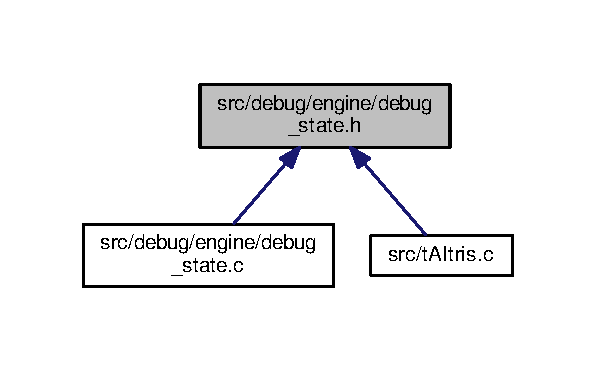
\includegraphics[width=286pt]{debug__state_8h__dep__incl}
\end{center}
\end{figure}
\subsection*{Macros}
\begin{DoxyCompactItemize}
\item 
\#define \textbf{ D\+E\+B\+U\+G\+\_\+\+S\+T\+A\+T\+E\+\_\+\+N\+A\+ME}~\char`\"{}State\char`\"{}
\item 
\#define \textbf{ D\+E\+B\+U\+G\+\_\+\+S\+T\+A\+T\+E\+\_\+\+C\+O\+L\+OR}~\textbf{ A\+N\+S\+I\+\_\+\+F\+G\+\_\+\+M\+A\+G\+E\+N\+TA}
\item 
\#define \textbf{ D\+E\+B\+U\+G\+\_\+\+S\+T\+A\+T\+E\+\_\+\+T\+AG}~\textbf{ D\+E\+B\+U\+G\+\_\+\+T\+AG}(\textbf{ D\+E\+B\+U\+G\+\_\+\+S\+T\+A\+T\+E\+\_\+\+N\+A\+ME}, \textbf{ D\+E\+B\+U\+G\+\_\+\+S\+T\+A\+T\+E\+\_\+\+C\+O\+L\+OR})
\end{DoxyCompactItemize}
\subsection*{Functions}
\begin{DoxyCompactItemize}
\item 
void \textbf{ debug\+\_\+state\+\_\+print\+\_\+line\+\_\+number} (const \textbf{ Board} $\ast$brd, int y)
\item 
void \textbf{ debug\+\_\+state\+\_\+print\+\_\+cell} (\textbf{ Cell} c)
\item 
void \textbf{ debug\+\_\+state\+\_\+print\+\_\+infos} (const \textbf{ State} $\ast$state, int y)
\item 
void \textbf{ debug\+\_\+state\+\_\+print\+\_\+next\+\_\+piece} (const \textbf{ Piece} $\ast$pc, int y)
\item 
void \textbf{ debug\+\_\+state\+\_\+print} (const \textbf{ State} $\ast$state)
\end{DoxyCompactItemize}


\subsection{Detailed Description}
Debug state. 

\begin{DoxyAuthor}{Author}
S4\+Master\+Race 
\end{DoxyAuthor}
\begin{DoxyVersion}{Version}
2.\+0 
\end{DoxyVersion}


\subsection{Macro Definition Documentation}
\mbox{\label{debug__state_8h_a96a34f31176781b762b4dd049da05bf1}} 
\index{debug\+\_\+state.\+h@{debug\+\_\+state.\+h}!D\+E\+B\+U\+G\+\_\+\+S\+T\+A\+T\+E\+\_\+\+C\+O\+L\+OR@{D\+E\+B\+U\+G\+\_\+\+S\+T\+A\+T\+E\+\_\+\+C\+O\+L\+OR}}
\index{D\+E\+B\+U\+G\+\_\+\+S\+T\+A\+T\+E\+\_\+\+C\+O\+L\+OR@{D\+E\+B\+U\+G\+\_\+\+S\+T\+A\+T\+E\+\_\+\+C\+O\+L\+OR}!debug\+\_\+state.\+h@{debug\+\_\+state.\+h}}
\subsubsection{D\+E\+B\+U\+G\+\_\+\+S\+T\+A\+T\+E\+\_\+\+C\+O\+L\+OR}
{\footnotesize\ttfamily \#define D\+E\+B\+U\+G\+\_\+\+S\+T\+A\+T\+E\+\_\+\+C\+O\+L\+OR~\textbf{ A\+N\+S\+I\+\_\+\+F\+G\+\_\+\+M\+A\+G\+E\+N\+TA}}

\mbox{\label{debug__state_8h_a3b9c262bd097061edd4266a0dae7ce2d}} 
\index{debug\+\_\+state.\+h@{debug\+\_\+state.\+h}!D\+E\+B\+U\+G\+\_\+\+S\+T\+A\+T\+E\+\_\+\+N\+A\+ME@{D\+E\+B\+U\+G\+\_\+\+S\+T\+A\+T\+E\+\_\+\+N\+A\+ME}}
\index{D\+E\+B\+U\+G\+\_\+\+S\+T\+A\+T\+E\+\_\+\+N\+A\+ME@{D\+E\+B\+U\+G\+\_\+\+S\+T\+A\+T\+E\+\_\+\+N\+A\+ME}!debug\+\_\+state.\+h@{debug\+\_\+state.\+h}}
\subsubsection{D\+E\+B\+U\+G\+\_\+\+S\+T\+A\+T\+E\+\_\+\+N\+A\+ME}
{\footnotesize\ttfamily \#define D\+E\+B\+U\+G\+\_\+\+S\+T\+A\+T\+E\+\_\+\+N\+A\+ME~\char`\"{}State\char`\"{}}

\mbox{\label{debug__state_8h_adc72047d6fcea722db2455b3af73bdd3}} 
\index{debug\+\_\+state.\+h@{debug\+\_\+state.\+h}!D\+E\+B\+U\+G\+\_\+\+S\+T\+A\+T\+E\+\_\+\+T\+AG@{D\+E\+B\+U\+G\+\_\+\+S\+T\+A\+T\+E\+\_\+\+T\+AG}}
\index{D\+E\+B\+U\+G\+\_\+\+S\+T\+A\+T\+E\+\_\+\+T\+AG@{D\+E\+B\+U\+G\+\_\+\+S\+T\+A\+T\+E\+\_\+\+T\+AG}!debug\+\_\+state.\+h@{debug\+\_\+state.\+h}}
\subsubsection{D\+E\+B\+U\+G\+\_\+\+S\+T\+A\+T\+E\+\_\+\+T\+AG}
{\footnotesize\ttfamily \#define D\+E\+B\+U\+G\+\_\+\+S\+T\+A\+T\+E\+\_\+\+T\+AG~\textbf{ D\+E\+B\+U\+G\+\_\+\+T\+AG}(\textbf{ D\+E\+B\+U\+G\+\_\+\+S\+T\+A\+T\+E\+\_\+\+N\+A\+ME}, \textbf{ D\+E\+B\+U\+G\+\_\+\+S\+T\+A\+T\+E\+\_\+\+C\+O\+L\+OR})}



\subsection{Function Documentation}
\mbox{\label{debug__state_8h_a9c0699f48870100dee7ceaa45763dd16}} 
\index{debug\+\_\+state.\+h@{debug\+\_\+state.\+h}!debug\+\_\+state\+\_\+print@{debug\+\_\+state\+\_\+print}}
\index{debug\+\_\+state\+\_\+print@{debug\+\_\+state\+\_\+print}!debug\+\_\+state.\+h@{debug\+\_\+state.\+h}}
\subsubsection{debug\+\_\+state\+\_\+print()}
{\footnotesize\ttfamily void debug\+\_\+state\+\_\+print (\begin{DoxyParamCaption}\item[{const \textbf{ State} $\ast$}]{state }\end{DoxyParamCaption})}

\mbox{\label{debug__state_8h_a57bffc683e10d64829dfaee65aa44c99}} 
\index{debug\+\_\+state.\+h@{debug\+\_\+state.\+h}!debug\+\_\+state\+\_\+print\+\_\+cell@{debug\+\_\+state\+\_\+print\+\_\+cell}}
\index{debug\+\_\+state\+\_\+print\+\_\+cell@{debug\+\_\+state\+\_\+print\+\_\+cell}!debug\+\_\+state.\+h@{debug\+\_\+state.\+h}}
\subsubsection{debug\+\_\+state\+\_\+print\+\_\+cell()}
{\footnotesize\ttfamily void debug\+\_\+state\+\_\+print\+\_\+cell (\begin{DoxyParamCaption}\item[{\textbf{ Cell}}]{c }\end{DoxyParamCaption})}

\mbox{\label{debug__state_8h_aa72d3737296f3a5b97a6589dc5cd8a92}} 
\index{debug\+\_\+state.\+h@{debug\+\_\+state.\+h}!debug\+\_\+state\+\_\+print\+\_\+infos@{debug\+\_\+state\+\_\+print\+\_\+infos}}
\index{debug\+\_\+state\+\_\+print\+\_\+infos@{debug\+\_\+state\+\_\+print\+\_\+infos}!debug\+\_\+state.\+h@{debug\+\_\+state.\+h}}
\subsubsection{debug\+\_\+state\+\_\+print\+\_\+infos()}
{\footnotesize\ttfamily void debug\+\_\+state\+\_\+print\+\_\+infos (\begin{DoxyParamCaption}\item[{const \textbf{ State} $\ast$}]{state,  }\item[{int}]{y }\end{DoxyParamCaption})}

\mbox{\label{debug__state_8h_a068cc3486e3c89355ca784fdb55194b4}} 
\index{debug\+\_\+state.\+h@{debug\+\_\+state.\+h}!debug\+\_\+state\+\_\+print\+\_\+line\+\_\+number@{debug\+\_\+state\+\_\+print\+\_\+line\+\_\+number}}
\index{debug\+\_\+state\+\_\+print\+\_\+line\+\_\+number@{debug\+\_\+state\+\_\+print\+\_\+line\+\_\+number}!debug\+\_\+state.\+h@{debug\+\_\+state.\+h}}
\subsubsection{debug\+\_\+state\+\_\+print\+\_\+line\+\_\+number()}
{\footnotesize\ttfamily void debug\+\_\+state\+\_\+print\+\_\+line\+\_\+number (\begin{DoxyParamCaption}\item[{const \textbf{ Board} $\ast$}]{brd,  }\item[{int}]{y }\end{DoxyParamCaption})}

\mbox{\label{debug__state_8h_ad288c47f98f24b9d84b889182a207256}} 
\index{debug\+\_\+state.\+h@{debug\+\_\+state.\+h}!debug\+\_\+state\+\_\+print\+\_\+next\+\_\+piece@{debug\+\_\+state\+\_\+print\+\_\+next\+\_\+piece}}
\index{debug\+\_\+state\+\_\+print\+\_\+next\+\_\+piece@{debug\+\_\+state\+\_\+print\+\_\+next\+\_\+piece}!debug\+\_\+state.\+h@{debug\+\_\+state.\+h}}
\subsubsection{debug\+\_\+state\+\_\+print\+\_\+next\+\_\+piece()}
{\footnotesize\ttfamily void debug\+\_\+state\+\_\+print\+\_\+next\+\_\+piece (\begin{DoxyParamCaption}\item[{const \textbf{ Piece} $\ast$}]{pc,  }\item[{int}]{y }\end{DoxyParamCaption})}


\section{src/engine/angle.h File Reference}
\label{angle_8h}\index{src/engine/angle.\+h@{src/engine/angle.\+h}}


Angle.  


This graph shows which files directly or indirectly include this file\+:
\nopagebreak
\begin{figure}[H]
\begin{center}
\leavevmode
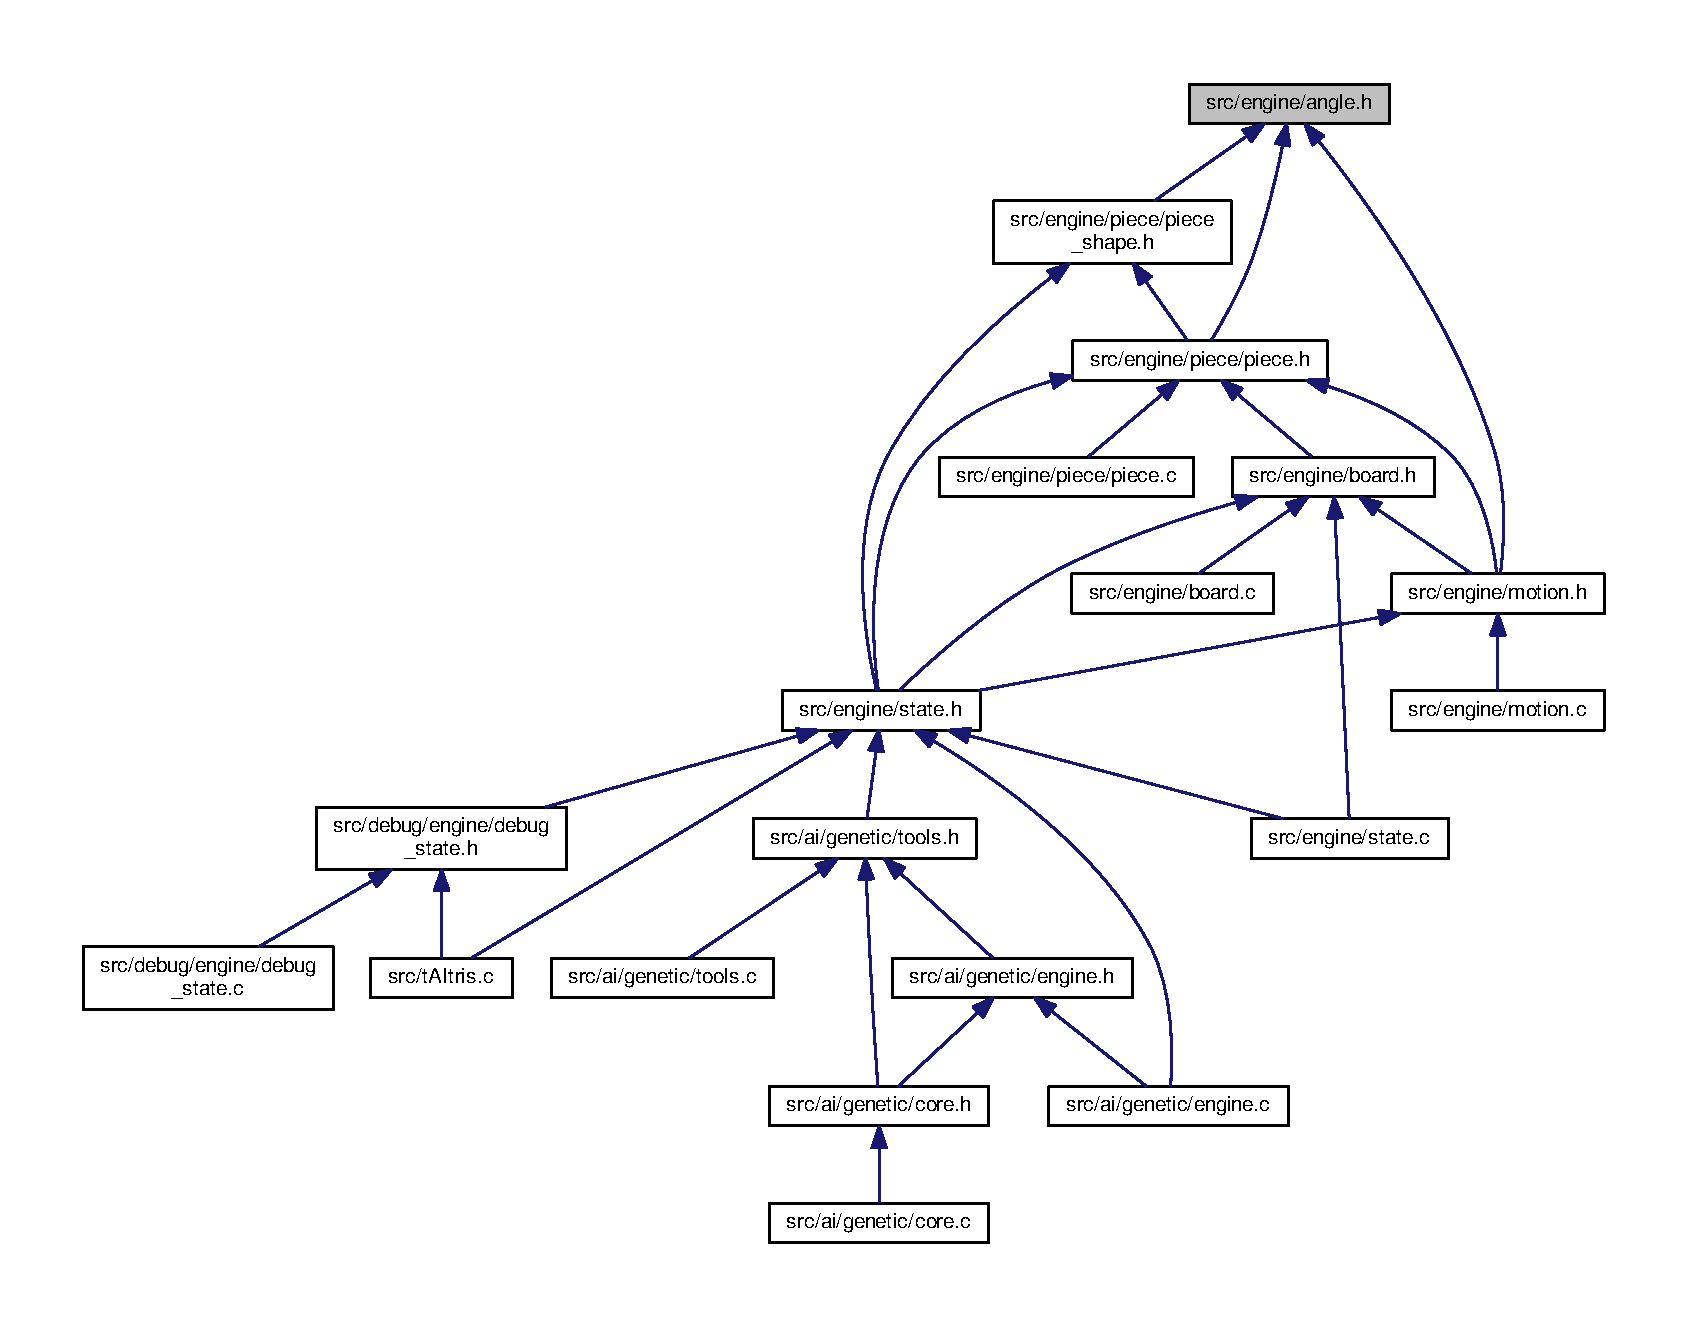
\includegraphics[width=350pt]{angle_8h__dep__incl}
\end{center}
\end{figure}
\subsection*{Macros}
\begin{DoxyCompactItemize}
\item 
\#define \textbf{ A\+N\+G\+L\+E\+\_\+\+E\+S\+I\+ZE}~4
\end{DoxyCompactItemize}
\subsection*{Enumerations}
\begin{DoxyCompactItemize}
\item 
enum \textbf{ Angle} \{ \textbf{ A\+N\+G\+L\+E\+\_\+\+UP}, 
\textbf{ A\+N\+G\+L\+E\+\_\+\+R\+I\+G\+HT}, 
\textbf{ A\+N\+G\+L\+E\+\_\+\+D\+O\+WN}, 
\textbf{ A\+N\+G\+L\+E\+\_\+\+L\+E\+FT}
 \}
\item 
enum \textbf{ Rotation} \{ \textbf{ R\+O\+T\+A\+T\+E\+\_\+\+L\+E\+FT} = -\/1, 
\textbf{ R\+O\+T\+A\+T\+E\+\_\+\+R\+I\+G\+HT} = 1
 \}
\end{DoxyCompactItemize}


\subsection{Detailed Description}
Angle. 

\begin{DoxyAuthor}{Author}
S4\+Master\+Race 
\end{DoxyAuthor}
\begin{DoxyVersion}{Version}
2.\+0 
\end{DoxyVersion}


\subsection{Macro Definition Documentation}
\mbox{\label{angle_8h_ac2a4e92ac8bd9e08ab1aace9b8cc4882}} 
\index{angle.\+h@{angle.\+h}!A\+N\+G\+L\+E\+\_\+\+E\+S\+I\+ZE@{A\+N\+G\+L\+E\+\_\+\+E\+S\+I\+ZE}}
\index{A\+N\+G\+L\+E\+\_\+\+E\+S\+I\+ZE@{A\+N\+G\+L\+E\+\_\+\+E\+S\+I\+ZE}!angle.\+h@{angle.\+h}}
\subsubsection{A\+N\+G\+L\+E\+\_\+\+E\+S\+I\+ZE}
{\footnotesize\ttfamily \#define A\+N\+G\+L\+E\+\_\+\+E\+S\+I\+ZE~4}



\subsection{Enumeration Type Documentation}
\mbox{\label{angle_8h_a0200d2d1b3a7930d0be6c50e7c8ae7d1}} 
\index{angle.\+h@{angle.\+h}!Angle@{Angle}}
\index{Angle@{Angle}!angle.\+h@{angle.\+h}}
\subsubsection{Angle}
{\footnotesize\ttfamily enum \textbf{ Angle}}

\begin{DoxyEnumFields}{Enumerator}
\raisebox{\heightof{T}}[0pt][0pt]{\index{A\+N\+G\+L\+E\+\_\+\+UP@{A\+N\+G\+L\+E\+\_\+\+UP}!angle.\+h@{angle.\+h}}\index{angle.\+h@{angle.\+h}!A\+N\+G\+L\+E\+\_\+\+UP@{A\+N\+G\+L\+E\+\_\+\+UP}}}\mbox{\label{angle_8h_a0200d2d1b3a7930d0be6c50e7c8ae7d1a700d37bd5b8364931f74b1255814200e}} 
A\+N\+G\+L\+E\+\_\+\+UP&\\
\hline

\raisebox{\heightof{T}}[0pt][0pt]{\index{A\+N\+G\+L\+E\+\_\+\+R\+I\+G\+HT@{A\+N\+G\+L\+E\+\_\+\+R\+I\+G\+HT}!angle.\+h@{angle.\+h}}\index{angle.\+h@{angle.\+h}!A\+N\+G\+L\+E\+\_\+\+R\+I\+G\+HT@{A\+N\+G\+L\+E\+\_\+\+R\+I\+G\+HT}}}\mbox{\label{angle_8h_a0200d2d1b3a7930d0be6c50e7c8ae7d1a35df88dc50d0fcc87637727815748073}} 
A\+N\+G\+L\+E\+\_\+\+R\+I\+G\+HT&\\
\hline

\raisebox{\heightof{T}}[0pt][0pt]{\index{A\+N\+G\+L\+E\+\_\+\+D\+O\+WN@{A\+N\+G\+L\+E\+\_\+\+D\+O\+WN}!angle.\+h@{angle.\+h}}\index{angle.\+h@{angle.\+h}!A\+N\+G\+L\+E\+\_\+\+D\+O\+WN@{A\+N\+G\+L\+E\+\_\+\+D\+O\+WN}}}\mbox{\label{angle_8h_a0200d2d1b3a7930d0be6c50e7c8ae7d1ad823a94306ee8ba0f028dba1a05be290}} 
A\+N\+G\+L\+E\+\_\+\+D\+O\+WN&\\
\hline

\raisebox{\heightof{T}}[0pt][0pt]{\index{A\+N\+G\+L\+E\+\_\+\+L\+E\+FT@{A\+N\+G\+L\+E\+\_\+\+L\+E\+FT}!angle.\+h@{angle.\+h}}\index{angle.\+h@{angle.\+h}!A\+N\+G\+L\+E\+\_\+\+L\+E\+FT@{A\+N\+G\+L\+E\+\_\+\+L\+E\+FT}}}\mbox{\label{angle_8h_a0200d2d1b3a7930d0be6c50e7c8ae7d1aebc82fe613fe0006bd16b094ad9c2308}} 
A\+N\+G\+L\+E\+\_\+\+L\+E\+FT&\\
\hline

\end{DoxyEnumFields}
\mbox{\label{angle_8h_a4940d1dc528122726d2c8c475657e1a9}} 
\index{angle.\+h@{angle.\+h}!Rotation@{Rotation}}
\index{Rotation@{Rotation}!angle.\+h@{angle.\+h}}
\subsubsection{Rotation}
{\footnotesize\ttfamily enum \textbf{ Rotation}}

\begin{DoxyEnumFields}{Enumerator}
\raisebox{\heightof{T}}[0pt][0pt]{\index{R\+O\+T\+A\+T\+E\+\_\+\+L\+E\+FT@{R\+O\+T\+A\+T\+E\+\_\+\+L\+E\+FT}!angle.\+h@{angle.\+h}}\index{angle.\+h@{angle.\+h}!R\+O\+T\+A\+T\+E\+\_\+\+L\+E\+FT@{R\+O\+T\+A\+T\+E\+\_\+\+L\+E\+FT}}}\mbox{\label{angle_8h_a4940d1dc528122726d2c8c475657e1a9a4058a39e19c958e2d10d7297d0beaa72}} 
R\+O\+T\+A\+T\+E\+\_\+\+L\+E\+FT&\\
\hline

\raisebox{\heightof{T}}[0pt][0pt]{\index{R\+O\+T\+A\+T\+E\+\_\+\+R\+I\+G\+HT@{R\+O\+T\+A\+T\+E\+\_\+\+R\+I\+G\+HT}!angle.\+h@{angle.\+h}}\index{angle.\+h@{angle.\+h}!R\+O\+T\+A\+T\+E\+\_\+\+R\+I\+G\+HT@{R\+O\+T\+A\+T\+E\+\_\+\+R\+I\+G\+HT}}}\mbox{\label{angle_8h_a4940d1dc528122726d2c8c475657e1a9a94c535fb585c220b052a698d4d467e4c}} 
R\+O\+T\+A\+T\+E\+\_\+\+R\+I\+G\+HT&\\
\hline

\end{DoxyEnumFields}

\section{src/engine/board.c File Reference}
\label{board_8c}\index{src/engine/board.\+c@{src/engine/board.\+c}}


\doxyref{Board}{p.}{structBoard}.  


{\ttfamily \#include \char`\"{}board.\+h\char`\"{}}\newline
Include dependency graph for board.\+c\+:
\nopagebreak
\begin{figure}[H]
\begin{center}
\leavevmode
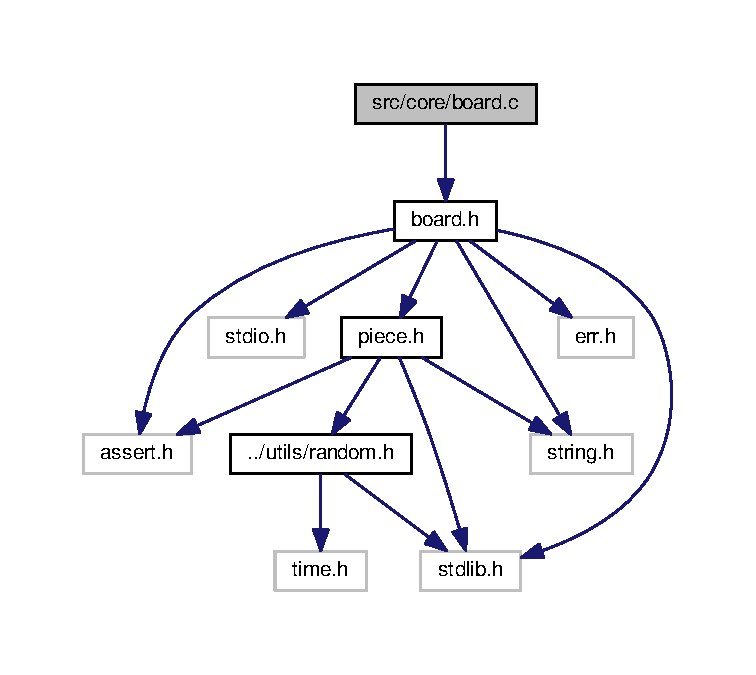
\includegraphics[width=350pt]{board_8c__incl}
\end{center}
\end{figure}
\subsection*{Functions}
\begin{DoxyCompactItemize}
\item 
\textbf{ Board} $\ast$ \textbf{ board\+\_\+create} (int width, int height)
\item 
void \textbf{ board\+\_\+init} (\textbf{ Board} $\ast$brd)
\item 
void \textbf{ board\+\_\+free} (\textbf{ Board} $\ast$brd)
\item 
\textbf{ Board} $\ast$ \textbf{ board\+\_\+copy} (\textbf{ Board} $\ast$brd)
\item 
size\+\_\+t \textbf{ board\+\_\+get\+\_\+completed\+\_\+lines} (const \textbf{ Board} $\ast$brd, int $\ast$hist)
\item 
void \textbf{ board\+\_\+break\+\_\+lines} (\textbf{ Board} $\ast$brd, const int $\ast$hist)
\item 
int \textbf{ board\+\_\+merge\+\_\+piece} (\textbf{ Board} $\ast$brd, const \textbf{ Piece} $\ast$pc)
\end{DoxyCompactItemize}


\subsection{Detailed Description}
\doxyref{Board}{p.}{structBoard}. 

\begin{DoxyAuthor}{Author}
S4\+Master\+Race 
\end{DoxyAuthor}
\begin{DoxyVersion}{Version}
2.\+0 
\end{DoxyVersion}


\subsection{Function Documentation}
\mbox{\label{board_8c_a6c85e1a231846cafebb7ac9f9bc3910a}} 
\index{board.\+c@{board.\+c}!board\+\_\+break\+\_\+lines@{board\+\_\+break\+\_\+lines}}
\index{board\+\_\+break\+\_\+lines@{board\+\_\+break\+\_\+lines}!board.\+c@{board.\+c}}
\subsubsection{board\+\_\+break\+\_\+lines()}
{\footnotesize\ttfamily void board\+\_\+break\+\_\+lines (\begin{DoxyParamCaption}\item[{\textbf{ Board} $\ast$}]{brd,  }\item[{const int $\ast$}]{hist }\end{DoxyParamCaption})}

\mbox{\label{board_8c_ac42ca212e2ffbc90b074b6a842c8ceb9}} 
\index{board.\+c@{board.\+c}!board\+\_\+copy@{board\+\_\+copy}}
\index{board\+\_\+copy@{board\+\_\+copy}!board.\+c@{board.\+c}}
\subsubsection{board\+\_\+copy()}
{\footnotesize\ttfamily \textbf{ Board}$\ast$ board\+\_\+copy (\begin{DoxyParamCaption}\item[{\textbf{ Board} $\ast$}]{brd }\end{DoxyParamCaption})}

\mbox{\label{board_8c_ae7e09c531608d7a5808f1c6b1d220770}} 
\index{board.\+c@{board.\+c}!board\+\_\+create@{board\+\_\+create}}
\index{board\+\_\+create@{board\+\_\+create}!board.\+c@{board.\+c}}
\subsubsection{board\+\_\+create()}
{\footnotesize\ttfamily \textbf{ Board}$\ast$ board\+\_\+create (\begin{DoxyParamCaption}\item[{int}]{width,  }\item[{int}]{height }\end{DoxyParamCaption})}

\mbox{\label{board_8c_a77b9336423c3e286f4456a4739dcad31}} 
\index{board.\+c@{board.\+c}!board\+\_\+free@{board\+\_\+free}}
\index{board\+\_\+free@{board\+\_\+free}!board.\+c@{board.\+c}}
\subsubsection{board\+\_\+free()}
{\footnotesize\ttfamily void board\+\_\+free (\begin{DoxyParamCaption}\item[{\textbf{ Board} $\ast$}]{brd }\end{DoxyParamCaption})}

\mbox{\label{board_8c_aafdfe55583b35684b3aeefce6047f1d6}} 
\index{board.\+c@{board.\+c}!board\+\_\+get\+\_\+completed\+\_\+lines@{board\+\_\+get\+\_\+completed\+\_\+lines}}
\index{board\+\_\+get\+\_\+completed\+\_\+lines@{board\+\_\+get\+\_\+completed\+\_\+lines}!board.\+c@{board.\+c}}
\subsubsection{board\+\_\+get\+\_\+completed\+\_\+lines()}
{\footnotesize\ttfamily size\+\_\+t board\+\_\+get\+\_\+completed\+\_\+lines (\begin{DoxyParamCaption}\item[{const \textbf{ Board} $\ast$}]{brd,  }\item[{int $\ast$}]{hist }\end{DoxyParamCaption})}

\mbox{\label{board_8c_a00449701ed118c6c9c907f3371b32921}} 
\index{board.\+c@{board.\+c}!board\+\_\+init@{board\+\_\+init}}
\index{board\+\_\+init@{board\+\_\+init}!board.\+c@{board.\+c}}
\subsubsection{board\+\_\+init()}
{\footnotesize\ttfamily void board\+\_\+init (\begin{DoxyParamCaption}\item[{\textbf{ Board} $\ast$}]{brd }\end{DoxyParamCaption})}

\mbox{\label{board_8c_acc71ac2aa1a547f8817ace71aad751ef}} 
\index{board.\+c@{board.\+c}!board\+\_\+merge\+\_\+piece@{board\+\_\+merge\+\_\+piece}}
\index{board\+\_\+merge\+\_\+piece@{board\+\_\+merge\+\_\+piece}!board.\+c@{board.\+c}}
\subsubsection{board\+\_\+merge\+\_\+piece()}
{\footnotesize\ttfamily int board\+\_\+merge\+\_\+piece (\begin{DoxyParamCaption}\item[{\textbf{ Board} $\ast$}]{brd,  }\item[{const \textbf{ Piece} $\ast$}]{pc }\end{DoxyParamCaption})}


\section{src/engine/board.h File Reference}
\label{board_8h}\index{src/engine/board.\+h@{src/engine/board.\+h}}


\doxyref{Board}{p.}{structBoard}.  


{\ttfamily \#include $<$stdlib.\+h$>$}\newline
{\ttfamily \#include $<$assert.\+h$>$}\newline
{\ttfamily \#include $<$string.\+h$>$}\newline
{\ttfamily \#include $<$err.\+h$>$}\newline
{\ttfamily \#include \char`\"{}piece/piece.\+h\char`\"{}}\newline
{\ttfamily \#include \char`\"{}cell.\+h\char`\"{}}\newline
Include dependency graph for board.\+h\+:
\nopagebreak
\begin{figure}[H]
\begin{center}
\leavevmode
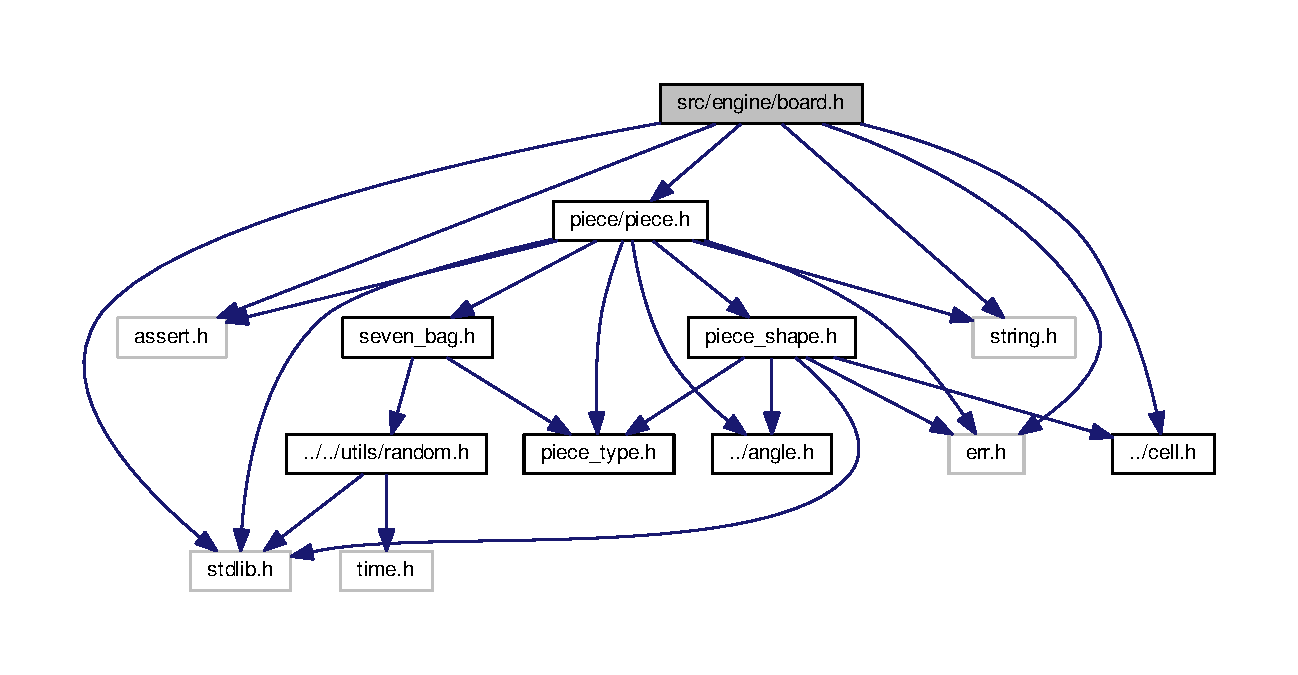
\includegraphics[width=350pt]{board_8h__incl}
\end{center}
\end{figure}
This graph shows which files directly or indirectly include this file\+:
\nopagebreak
\begin{figure}[H]
\begin{center}
\leavevmode
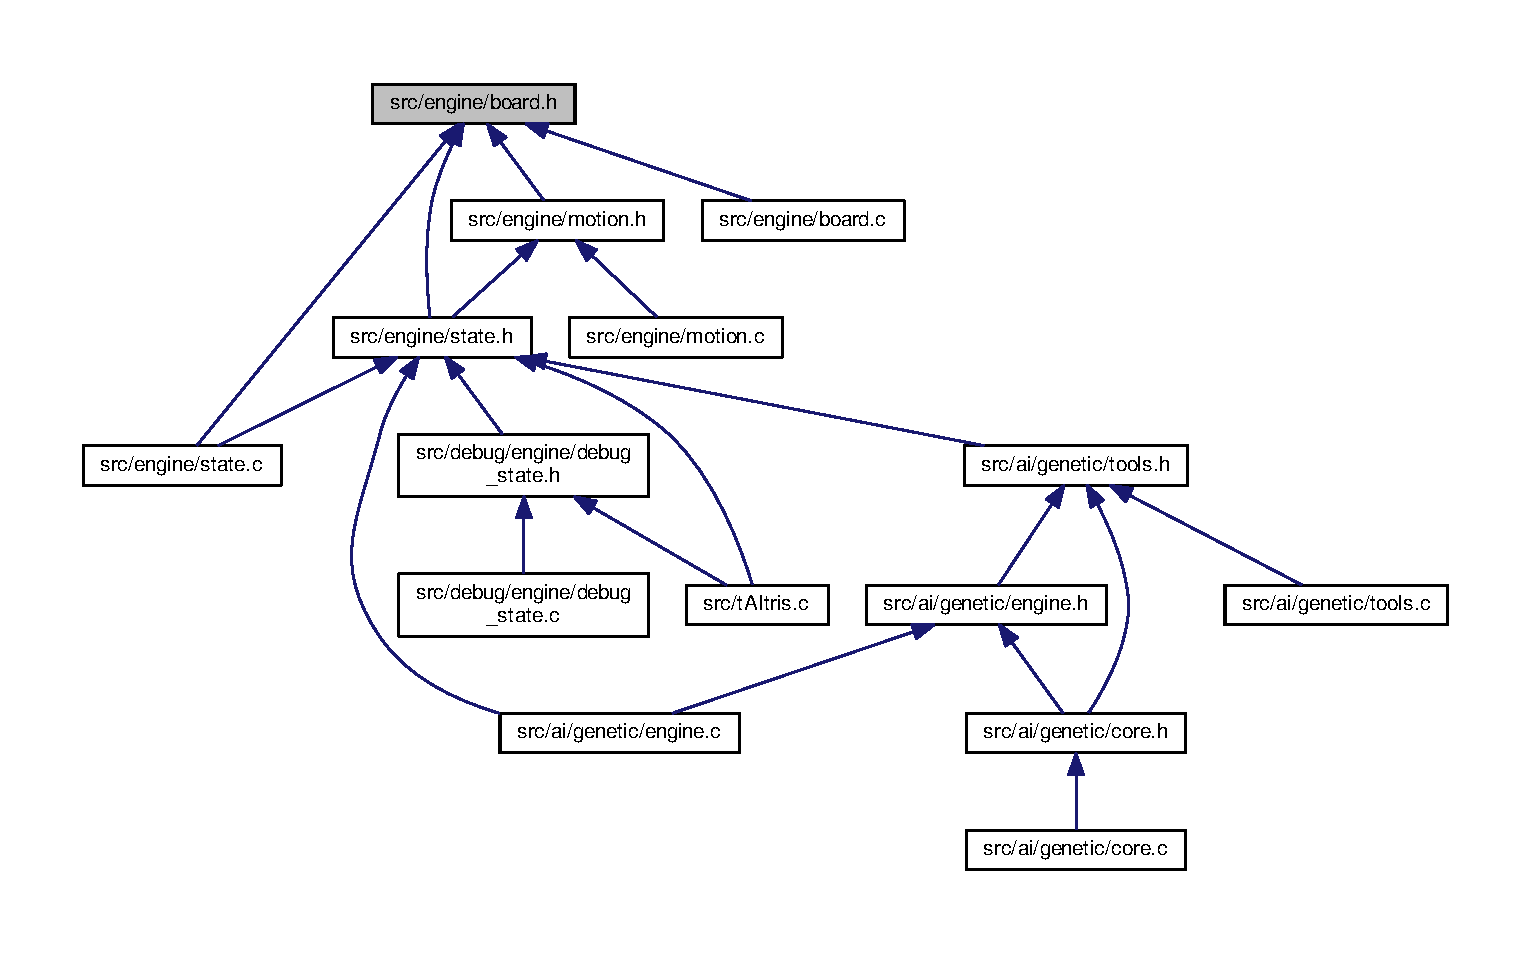
\includegraphics[width=350pt]{board_8h__dep__incl}
\end{center}
\end{figure}
\subsection*{Data Structures}
\begin{DoxyCompactItemize}
\item 
struct \textbf{ Board}
\end{DoxyCompactItemize}
\subsection*{Macros}
\begin{DoxyCompactItemize}
\item 
\#define \textbf{ B\+O\+A\+R\+D\+\_\+\+W\+I\+D\+TH}~10
\item 
\#define \textbf{ B\+O\+A\+R\+D\+\_\+\+H\+E\+I\+G\+HT}~20
\item 
\#define \textbf{ B\+O\+A\+R\+D\+\_\+\+H\+I\+D\+D\+EN}~2
\item 
\#define \textbf{ board\+\_\+reverse\+\_\+y}(\+\_\+brd\+\_\+,  \+\_\+y\+\_\+)~((\+\_\+brd\+\_\+)-\/$>$height -\/ 1 -\/ (\+\_\+y\+\_\+))
\end{DoxyCompactItemize}
\subsection*{Functions}
\begin{DoxyCompactItemize}
\item 
\textbf{ Board} $\ast$ \textbf{ board\+\_\+create} (int width, int height)
\item 
void \textbf{ board\+\_\+init} (\textbf{ Board} $\ast$brd)
\item 
void \textbf{ board\+\_\+free} (\textbf{ Board} $\ast$brd)
\item 
\textbf{ Board} $\ast$ \textbf{ board\+\_\+copy} (\textbf{ Board} $\ast$brd)
\item 
size\+\_\+t \textbf{ board\+\_\+get\+\_\+completed\+\_\+lines} (const \textbf{ Board} $\ast$brd, int $\ast$hist)
\item 
void \textbf{ board\+\_\+break\+\_\+lines} (\textbf{ Board} $\ast$brd, const int $\ast$hist)
\item 
int \textbf{ board\+\_\+merge\+\_\+piece} (\textbf{ Board} $\ast$brd, const \textbf{ Piece} $\ast$pc)
\end{DoxyCompactItemize}


\subsection{Detailed Description}
\doxyref{Board}{p.}{structBoard}. 

\begin{DoxyAuthor}{Author}
S4\+Master\+Race 
\end{DoxyAuthor}
\begin{DoxyVersion}{Version}
2.\+0 
\end{DoxyVersion}


\subsection{Macro Definition Documentation}
\mbox{\label{board_8h_a94ed08e31d2f3a38d35f0cb89c762f04}} 
\index{board.\+h@{board.\+h}!B\+O\+A\+R\+D\+\_\+\+H\+E\+I\+G\+HT@{B\+O\+A\+R\+D\+\_\+\+H\+E\+I\+G\+HT}}
\index{B\+O\+A\+R\+D\+\_\+\+H\+E\+I\+G\+HT@{B\+O\+A\+R\+D\+\_\+\+H\+E\+I\+G\+HT}!board.\+h@{board.\+h}}
\subsubsection{B\+O\+A\+R\+D\+\_\+\+H\+E\+I\+G\+HT}
{\footnotesize\ttfamily \#define B\+O\+A\+R\+D\+\_\+\+H\+E\+I\+G\+HT~20}

\mbox{\label{board_8h_abf8d33781dfc8022f53a68678602fd10}} 
\index{board.\+h@{board.\+h}!B\+O\+A\+R\+D\+\_\+\+H\+I\+D\+D\+EN@{B\+O\+A\+R\+D\+\_\+\+H\+I\+D\+D\+EN}}
\index{B\+O\+A\+R\+D\+\_\+\+H\+I\+D\+D\+EN@{B\+O\+A\+R\+D\+\_\+\+H\+I\+D\+D\+EN}!board.\+h@{board.\+h}}
\subsubsection{B\+O\+A\+R\+D\+\_\+\+H\+I\+D\+D\+EN}
{\footnotesize\ttfamily \#define B\+O\+A\+R\+D\+\_\+\+H\+I\+D\+D\+EN~2}

\mbox{\label{board_8h_a2497487ce0ccce0841ea57cb4b7fc020}} 
\index{board.\+h@{board.\+h}!board\+\_\+reverse\+\_\+y@{board\+\_\+reverse\+\_\+y}}
\index{board\+\_\+reverse\+\_\+y@{board\+\_\+reverse\+\_\+y}!board.\+h@{board.\+h}}
\subsubsection{board\+\_\+reverse\+\_\+y}
{\footnotesize\ttfamily \#define board\+\_\+reverse\+\_\+y(\begin{DoxyParamCaption}\item[{}]{\+\_\+brd\+\_\+,  }\item[{}]{\+\_\+y\+\_\+ }\end{DoxyParamCaption})~((\+\_\+brd\+\_\+)-\/$>$height -\/ 1 -\/ (\+\_\+y\+\_\+))}

\mbox{\label{board_8h_a1cd139e8d1f7ae83f54c8d477313d8ea}} 
\index{board.\+h@{board.\+h}!B\+O\+A\+R\+D\+\_\+\+W\+I\+D\+TH@{B\+O\+A\+R\+D\+\_\+\+W\+I\+D\+TH}}
\index{B\+O\+A\+R\+D\+\_\+\+W\+I\+D\+TH@{B\+O\+A\+R\+D\+\_\+\+W\+I\+D\+TH}!board.\+h@{board.\+h}}
\subsubsection{B\+O\+A\+R\+D\+\_\+\+W\+I\+D\+TH}
{\footnotesize\ttfamily \#define B\+O\+A\+R\+D\+\_\+\+W\+I\+D\+TH~10}



\subsection{Function Documentation}
\mbox{\label{board_8h_a6c85e1a231846cafebb7ac9f9bc3910a}} 
\index{board.\+h@{board.\+h}!board\+\_\+break\+\_\+lines@{board\+\_\+break\+\_\+lines}}
\index{board\+\_\+break\+\_\+lines@{board\+\_\+break\+\_\+lines}!board.\+h@{board.\+h}}
\subsubsection{board\+\_\+break\+\_\+lines()}
{\footnotesize\ttfamily void board\+\_\+break\+\_\+lines (\begin{DoxyParamCaption}\item[{\textbf{ Board} $\ast$}]{brd,  }\item[{const int $\ast$}]{hist }\end{DoxyParamCaption})}

\mbox{\label{board_8h_ac42ca212e2ffbc90b074b6a842c8ceb9}} 
\index{board.\+h@{board.\+h}!board\+\_\+copy@{board\+\_\+copy}}
\index{board\+\_\+copy@{board\+\_\+copy}!board.\+h@{board.\+h}}
\subsubsection{board\+\_\+copy()}
{\footnotesize\ttfamily \textbf{ Board}$\ast$ board\+\_\+copy (\begin{DoxyParamCaption}\item[{\textbf{ Board} $\ast$}]{brd }\end{DoxyParamCaption})}

\mbox{\label{board_8h_ae7e09c531608d7a5808f1c6b1d220770}} 
\index{board.\+h@{board.\+h}!board\+\_\+create@{board\+\_\+create}}
\index{board\+\_\+create@{board\+\_\+create}!board.\+h@{board.\+h}}
\subsubsection{board\+\_\+create()}
{\footnotesize\ttfamily \textbf{ Board}$\ast$ board\+\_\+create (\begin{DoxyParamCaption}\item[{int}]{width,  }\item[{int}]{height }\end{DoxyParamCaption})}

\mbox{\label{board_8h_a77b9336423c3e286f4456a4739dcad31}} 
\index{board.\+h@{board.\+h}!board\+\_\+free@{board\+\_\+free}}
\index{board\+\_\+free@{board\+\_\+free}!board.\+h@{board.\+h}}
\subsubsection{board\+\_\+free()}
{\footnotesize\ttfamily void board\+\_\+free (\begin{DoxyParamCaption}\item[{\textbf{ Board} $\ast$}]{brd }\end{DoxyParamCaption})}

\mbox{\label{board_8h_aafdfe55583b35684b3aeefce6047f1d6}} 
\index{board.\+h@{board.\+h}!board\+\_\+get\+\_\+completed\+\_\+lines@{board\+\_\+get\+\_\+completed\+\_\+lines}}
\index{board\+\_\+get\+\_\+completed\+\_\+lines@{board\+\_\+get\+\_\+completed\+\_\+lines}!board.\+h@{board.\+h}}
\subsubsection{board\+\_\+get\+\_\+completed\+\_\+lines()}
{\footnotesize\ttfamily size\+\_\+t board\+\_\+get\+\_\+completed\+\_\+lines (\begin{DoxyParamCaption}\item[{const \textbf{ Board} $\ast$}]{brd,  }\item[{int $\ast$}]{hist }\end{DoxyParamCaption})}

\mbox{\label{board_8h_a00449701ed118c6c9c907f3371b32921}} 
\index{board.\+h@{board.\+h}!board\+\_\+init@{board\+\_\+init}}
\index{board\+\_\+init@{board\+\_\+init}!board.\+h@{board.\+h}}
\subsubsection{board\+\_\+init()}
{\footnotesize\ttfamily void board\+\_\+init (\begin{DoxyParamCaption}\item[{\textbf{ Board} $\ast$}]{brd }\end{DoxyParamCaption})}

\mbox{\label{board_8h_acc71ac2aa1a547f8817ace71aad751ef}} 
\index{board.\+h@{board.\+h}!board\+\_\+merge\+\_\+piece@{board\+\_\+merge\+\_\+piece}}
\index{board\+\_\+merge\+\_\+piece@{board\+\_\+merge\+\_\+piece}!board.\+h@{board.\+h}}
\subsubsection{board\+\_\+merge\+\_\+piece()}
{\footnotesize\ttfamily int board\+\_\+merge\+\_\+piece (\begin{DoxyParamCaption}\item[{\textbf{ Board} $\ast$}]{brd,  }\item[{const \textbf{ Piece} $\ast$}]{pc }\end{DoxyParamCaption})}


\section{src/engine/cell.h File Reference}
\label{cell_8h}\index{src/engine/cell.\+h@{src/engine/cell.\+h}}


Cell.  


This graph shows which files directly or indirectly include this file\+:
\nopagebreak
\begin{figure}[H]
\begin{center}
\leavevmode
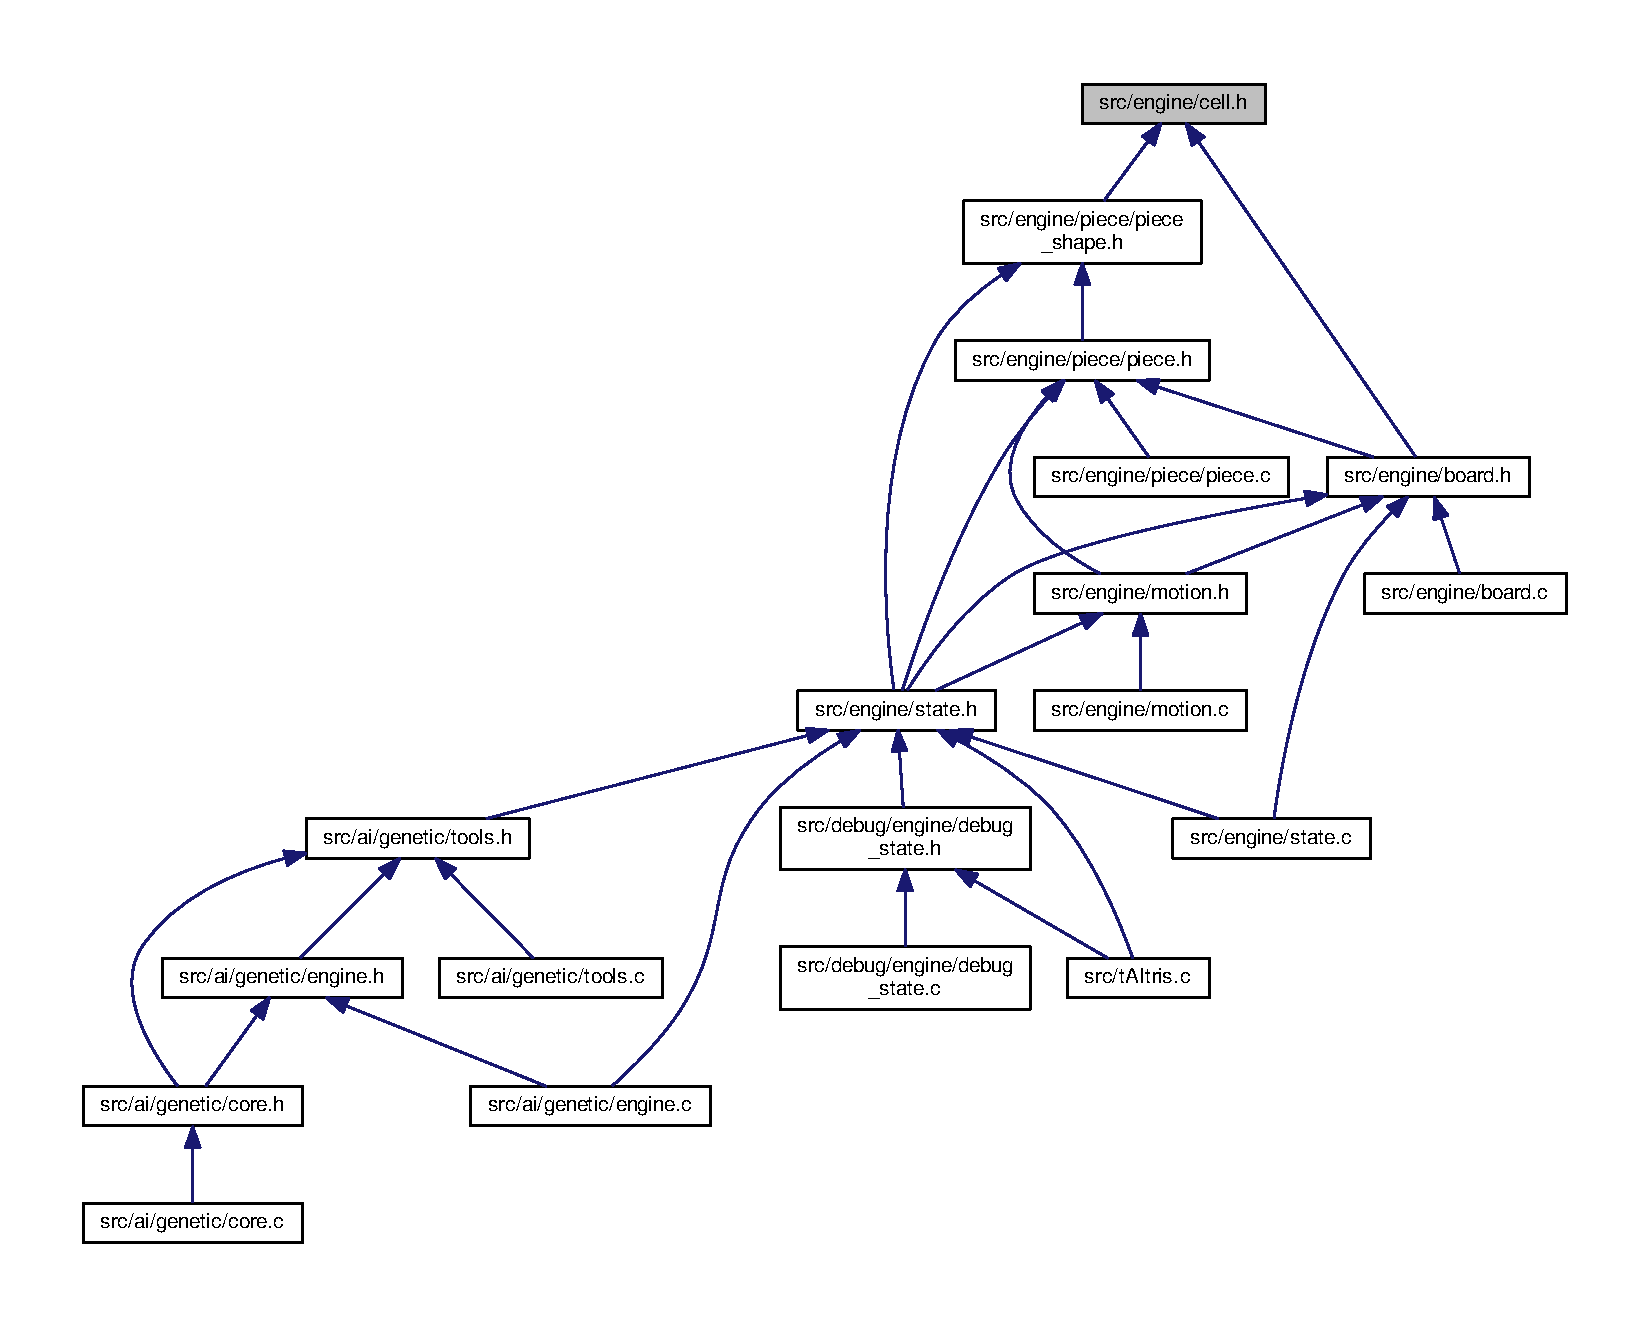
\includegraphics[width=350pt]{cell_8h__dep__incl}
\end{center}
\end{figure}
\subsection*{Macros}
\begin{DoxyCompactItemize}
\item 
\#define \textbf{ C\+E\+L\+L\+\_\+\+E\+S\+I\+ZE}~8
\end{DoxyCompactItemize}
\subsection*{Enumerations}
\begin{DoxyCompactItemize}
\item 
enum \textbf{ Cell} \{ \newline
\textbf{ C\+E\+L\+L\+\_\+\+E\+M\+P\+TY}, 
\textbf{ C\+E\+L\+L\+\_\+\+C\+Y\+AN}, 
\textbf{ C\+E\+L\+L\+\_\+\+Y\+E\+L\+L\+OW}, 
\textbf{ C\+E\+L\+L\+\_\+\+P\+U\+R\+P\+LE}, 
\newline
\textbf{ C\+E\+L\+L\+\_\+\+G\+R\+E\+EN}, 
\textbf{ C\+E\+L\+L\+\_\+\+R\+ED}, 
\textbf{ C\+E\+L\+L\+\_\+\+B\+L\+UE}, 
\textbf{ C\+E\+L\+L\+\_\+\+O\+R\+A\+N\+GE}
 \}
\end{DoxyCompactItemize}


\subsection{Detailed Description}
Cell. 

\begin{DoxyAuthor}{Author}
S4\+Master\+Race 
\end{DoxyAuthor}
\begin{DoxyVersion}{Version}
2.\+0 
\end{DoxyVersion}


\subsection{Macro Definition Documentation}
\mbox{\label{cell_8h_a87d2a1196530d0fb8198cb507229b1e2}} 
\index{cell.\+h@{cell.\+h}!C\+E\+L\+L\+\_\+\+E\+S\+I\+ZE@{C\+E\+L\+L\+\_\+\+E\+S\+I\+ZE}}
\index{C\+E\+L\+L\+\_\+\+E\+S\+I\+ZE@{C\+E\+L\+L\+\_\+\+E\+S\+I\+ZE}!cell.\+h@{cell.\+h}}
\subsubsection{C\+E\+L\+L\+\_\+\+E\+S\+I\+ZE}
{\footnotesize\ttfamily \#define C\+E\+L\+L\+\_\+\+E\+S\+I\+ZE~8}



\subsection{Enumeration Type Documentation}
\mbox{\label{cell_8h_a0133c02dfc35ffbaf07ad1a587dac4d1}} 
\index{cell.\+h@{cell.\+h}!Cell@{Cell}}
\index{Cell@{Cell}!cell.\+h@{cell.\+h}}
\subsubsection{Cell}
{\footnotesize\ttfamily enum \textbf{ Cell}}

\begin{DoxyEnumFields}{Enumerator}
\raisebox{\heightof{T}}[0pt][0pt]{\index{C\+E\+L\+L\+\_\+\+E\+M\+P\+TY@{C\+E\+L\+L\+\_\+\+E\+M\+P\+TY}!cell.\+h@{cell.\+h}}\index{cell.\+h@{cell.\+h}!C\+E\+L\+L\+\_\+\+E\+M\+P\+TY@{C\+E\+L\+L\+\_\+\+E\+M\+P\+TY}}}\mbox{\label{cell_8h_a0133c02dfc35ffbaf07ad1a587dac4d1a3d2f96279e71e38dbbd9782b48bf12fa}} 
C\+E\+L\+L\+\_\+\+E\+M\+P\+TY&\\
\hline

\raisebox{\heightof{T}}[0pt][0pt]{\index{C\+E\+L\+L\+\_\+\+C\+Y\+AN@{C\+E\+L\+L\+\_\+\+C\+Y\+AN}!cell.\+h@{cell.\+h}}\index{cell.\+h@{cell.\+h}!C\+E\+L\+L\+\_\+\+C\+Y\+AN@{C\+E\+L\+L\+\_\+\+C\+Y\+AN}}}\mbox{\label{cell_8h_a0133c02dfc35ffbaf07ad1a587dac4d1a51af70744ecd288930b4a716d43482a1}} 
C\+E\+L\+L\+\_\+\+C\+Y\+AN&\\
\hline

\raisebox{\heightof{T}}[0pt][0pt]{\index{C\+E\+L\+L\+\_\+\+Y\+E\+L\+L\+OW@{C\+E\+L\+L\+\_\+\+Y\+E\+L\+L\+OW}!cell.\+h@{cell.\+h}}\index{cell.\+h@{cell.\+h}!C\+E\+L\+L\+\_\+\+Y\+E\+L\+L\+OW@{C\+E\+L\+L\+\_\+\+Y\+E\+L\+L\+OW}}}\mbox{\label{cell_8h_a0133c02dfc35ffbaf07ad1a587dac4d1adff4817d99a86e6a2c08bc4ad4e43117}} 
C\+E\+L\+L\+\_\+\+Y\+E\+L\+L\+OW&\\
\hline

\raisebox{\heightof{T}}[0pt][0pt]{\index{C\+E\+L\+L\+\_\+\+P\+U\+R\+P\+LE@{C\+E\+L\+L\+\_\+\+P\+U\+R\+P\+LE}!cell.\+h@{cell.\+h}}\index{cell.\+h@{cell.\+h}!C\+E\+L\+L\+\_\+\+P\+U\+R\+P\+LE@{C\+E\+L\+L\+\_\+\+P\+U\+R\+P\+LE}}}\mbox{\label{cell_8h_a0133c02dfc35ffbaf07ad1a587dac4d1ae1873855c19f6070cc7cb4d55639140c}} 
C\+E\+L\+L\+\_\+\+P\+U\+R\+P\+LE&\\
\hline

\raisebox{\heightof{T}}[0pt][0pt]{\index{C\+E\+L\+L\+\_\+\+G\+R\+E\+EN@{C\+E\+L\+L\+\_\+\+G\+R\+E\+EN}!cell.\+h@{cell.\+h}}\index{cell.\+h@{cell.\+h}!C\+E\+L\+L\+\_\+\+G\+R\+E\+EN@{C\+E\+L\+L\+\_\+\+G\+R\+E\+EN}}}\mbox{\label{cell_8h_a0133c02dfc35ffbaf07ad1a587dac4d1a3212a147e8b4001e245159ed0e8a6d1b}} 
C\+E\+L\+L\+\_\+\+G\+R\+E\+EN&\\
\hline

\raisebox{\heightof{T}}[0pt][0pt]{\index{C\+E\+L\+L\+\_\+\+R\+ED@{C\+E\+L\+L\+\_\+\+R\+ED}!cell.\+h@{cell.\+h}}\index{cell.\+h@{cell.\+h}!C\+E\+L\+L\+\_\+\+R\+ED@{C\+E\+L\+L\+\_\+\+R\+ED}}}\mbox{\label{cell_8h_a0133c02dfc35ffbaf07ad1a587dac4d1a00b4e50030dda5ed3ec46b7e71053e4e}} 
C\+E\+L\+L\+\_\+\+R\+ED&\\
\hline

\raisebox{\heightof{T}}[0pt][0pt]{\index{C\+E\+L\+L\+\_\+\+B\+L\+UE@{C\+E\+L\+L\+\_\+\+B\+L\+UE}!cell.\+h@{cell.\+h}}\index{cell.\+h@{cell.\+h}!C\+E\+L\+L\+\_\+\+B\+L\+UE@{C\+E\+L\+L\+\_\+\+B\+L\+UE}}}\mbox{\label{cell_8h_a0133c02dfc35ffbaf07ad1a587dac4d1aefe191ebb208c15ea53cad6469d62221}} 
C\+E\+L\+L\+\_\+\+B\+L\+UE&\\
\hline

\raisebox{\heightof{T}}[0pt][0pt]{\index{C\+E\+L\+L\+\_\+\+O\+R\+A\+N\+GE@{C\+E\+L\+L\+\_\+\+O\+R\+A\+N\+GE}!cell.\+h@{cell.\+h}}\index{cell.\+h@{cell.\+h}!C\+E\+L\+L\+\_\+\+O\+R\+A\+N\+GE@{C\+E\+L\+L\+\_\+\+O\+R\+A\+N\+GE}}}\mbox{\label{cell_8h_a0133c02dfc35ffbaf07ad1a587dac4d1ad86d91f7b301b5256c2a85f17eada7ea}} 
C\+E\+L\+L\+\_\+\+O\+R\+A\+N\+GE&\\
\hline

\end{DoxyEnumFields}

\section{src/engine/input.h File Reference}
\label{input_8h}\index{src/engine/input.\+h@{src/engine/input.\+h}}


Input.  


This graph shows which files directly or indirectly include this file\+:
\nopagebreak
\begin{figure}[H]
\begin{center}
\leavevmode
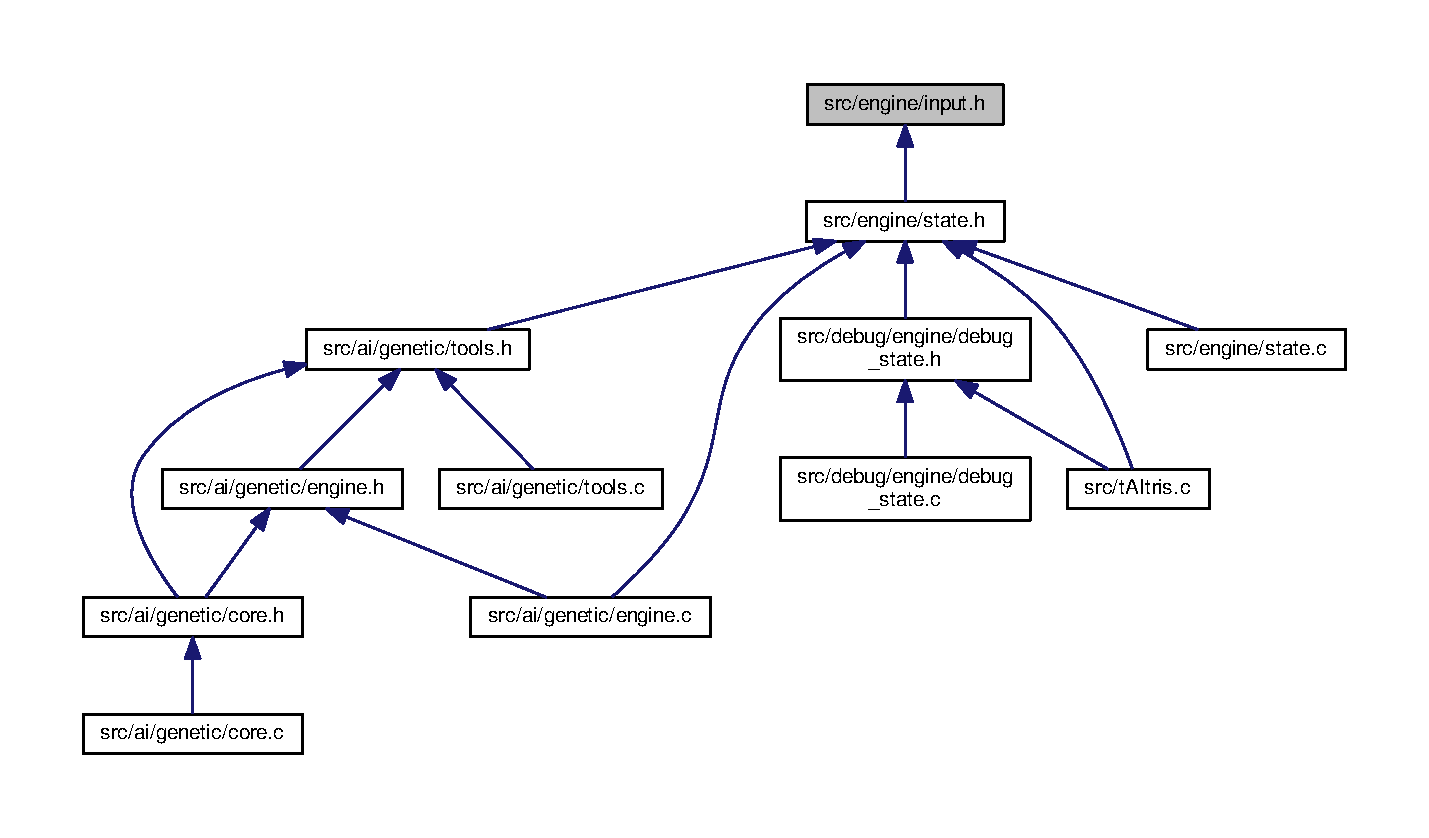
\includegraphics[width=350pt]{input_8h__dep__incl}
\end{center}
\end{figure}
\subsection*{Macros}
\begin{DoxyCompactItemize}
\item 
\#define \textbf{ I\+N\+P\+U\+T\+\_\+\+E\+S\+I\+ZE}~6
\end{DoxyCompactItemize}
\subsection*{Enumerations}
\begin{DoxyCompactItemize}
\item 
enum \textbf{ Input} \{ \newline
\textbf{ I\+N\+P\+U\+T\+\_\+\+M\+O\+V\+E\+\_\+\+L\+E\+FT}, 
\textbf{ I\+N\+P\+U\+T\+\_\+\+M\+O\+V\+E\+\_\+\+R\+I\+G\+HT}, 
\textbf{ I\+N\+P\+U\+T\+\_\+\+R\+O\+T\+A\+T\+E\+\_\+\+R\+I\+G\+HT}, 
\textbf{ I\+N\+P\+U\+T\+\_\+\+R\+O\+T\+A\+T\+E\+\_\+\+L\+E\+FT}, 
\newline
\textbf{ I\+N\+P\+U\+T\+\_\+\+S\+O\+F\+T\+\_\+\+D\+R\+OP}, 
\textbf{ I\+N\+P\+U\+T\+\_\+\+H\+A\+R\+D\+\_\+\+D\+R\+OP}
 \}
\end{DoxyCompactItemize}


\subsection{Detailed Description}
Input. 

\begin{DoxyAuthor}{Author}
S4\+Master\+Race 
\end{DoxyAuthor}
\begin{DoxyVersion}{Version}
2.\+0 
\end{DoxyVersion}


\subsection{Macro Definition Documentation}
\mbox{\label{input_8h_a2737fc7864bdc5313f58375cf0e56cd5}} 
\index{input.\+h@{input.\+h}!I\+N\+P\+U\+T\+\_\+\+E\+S\+I\+ZE@{I\+N\+P\+U\+T\+\_\+\+E\+S\+I\+ZE}}
\index{I\+N\+P\+U\+T\+\_\+\+E\+S\+I\+ZE@{I\+N\+P\+U\+T\+\_\+\+E\+S\+I\+ZE}!input.\+h@{input.\+h}}
\subsubsection{I\+N\+P\+U\+T\+\_\+\+E\+S\+I\+ZE}
{\footnotesize\ttfamily \#define I\+N\+P\+U\+T\+\_\+\+E\+S\+I\+ZE~6}



\subsection{Enumeration Type Documentation}
\mbox{\label{input_8h_a080a822f0093973313bd644e517a5090}} 
\index{input.\+h@{input.\+h}!Input@{Input}}
\index{Input@{Input}!input.\+h@{input.\+h}}
\subsubsection{Input}
{\footnotesize\ttfamily enum \textbf{ Input}}

\begin{DoxyEnumFields}{Enumerator}
\raisebox{\heightof{T}}[0pt][0pt]{\index{I\+N\+P\+U\+T\+\_\+\+M\+O\+V\+E\+\_\+\+L\+E\+FT@{I\+N\+P\+U\+T\+\_\+\+M\+O\+V\+E\+\_\+\+L\+E\+FT}!input.\+h@{input.\+h}}\index{input.\+h@{input.\+h}!I\+N\+P\+U\+T\+\_\+\+M\+O\+V\+E\+\_\+\+L\+E\+FT@{I\+N\+P\+U\+T\+\_\+\+M\+O\+V\+E\+\_\+\+L\+E\+FT}}}\mbox{\label{input_8h_a080a822f0093973313bd644e517a5090ac918452e1e902bee957d64a9ac857614}} 
I\+N\+P\+U\+T\+\_\+\+M\+O\+V\+E\+\_\+\+L\+E\+FT&\\
\hline

\raisebox{\heightof{T}}[0pt][0pt]{\index{I\+N\+P\+U\+T\+\_\+\+M\+O\+V\+E\+\_\+\+R\+I\+G\+HT@{I\+N\+P\+U\+T\+\_\+\+M\+O\+V\+E\+\_\+\+R\+I\+G\+HT}!input.\+h@{input.\+h}}\index{input.\+h@{input.\+h}!I\+N\+P\+U\+T\+\_\+\+M\+O\+V\+E\+\_\+\+R\+I\+G\+HT@{I\+N\+P\+U\+T\+\_\+\+M\+O\+V\+E\+\_\+\+R\+I\+G\+HT}}}\mbox{\label{input_8h_a080a822f0093973313bd644e517a5090aa6ac3dbfc2de686ba904cd66f7488fdb}} 
I\+N\+P\+U\+T\+\_\+\+M\+O\+V\+E\+\_\+\+R\+I\+G\+HT&\\
\hline

\raisebox{\heightof{T}}[0pt][0pt]{\index{I\+N\+P\+U\+T\+\_\+\+R\+O\+T\+A\+T\+E\+\_\+\+R\+I\+G\+HT@{I\+N\+P\+U\+T\+\_\+\+R\+O\+T\+A\+T\+E\+\_\+\+R\+I\+G\+HT}!input.\+h@{input.\+h}}\index{input.\+h@{input.\+h}!I\+N\+P\+U\+T\+\_\+\+R\+O\+T\+A\+T\+E\+\_\+\+R\+I\+G\+HT@{I\+N\+P\+U\+T\+\_\+\+R\+O\+T\+A\+T\+E\+\_\+\+R\+I\+G\+HT}}}\mbox{\label{input_8h_a080a822f0093973313bd644e517a5090a5007574ac4de084bd28c4c9fafd22d9b}} 
I\+N\+P\+U\+T\+\_\+\+R\+O\+T\+A\+T\+E\+\_\+\+R\+I\+G\+HT&\\
\hline

\raisebox{\heightof{T}}[0pt][0pt]{\index{I\+N\+P\+U\+T\+\_\+\+R\+O\+T\+A\+T\+E\+\_\+\+L\+E\+FT@{I\+N\+P\+U\+T\+\_\+\+R\+O\+T\+A\+T\+E\+\_\+\+L\+E\+FT}!input.\+h@{input.\+h}}\index{input.\+h@{input.\+h}!I\+N\+P\+U\+T\+\_\+\+R\+O\+T\+A\+T\+E\+\_\+\+L\+E\+FT@{I\+N\+P\+U\+T\+\_\+\+R\+O\+T\+A\+T\+E\+\_\+\+L\+E\+FT}}}\mbox{\label{input_8h_a080a822f0093973313bd644e517a5090a1314047c6bf947caa826d0d2e53da39c}} 
I\+N\+P\+U\+T\+\_\+\+R\+O\+T\+A\+T\+E\+\_\+\+L\+E\+FT&\\
\hline

\raisebox{\heightof{T}}[0pt][0pt]{\index{I\+N\+P\+U\+T\+\_\+\+S\+O\+F\+T\+\_\+\+D\+R\+OP@{I\+N\+P\+U\+T\+\_\+\+S\+O\+F\+T\+\_\+\+D\+R\+OP}!input.\+h@{input.\+h}}\index{input.\+h@{input.\+h}!I\+N\+P\+U\+T\+\_\+\+S\+O\+F\+T\+\_\+\+D\+R\+OP@{I\+N\+P\+U\+T\+\_\+\+S\+O\+F\+T\+\_\+\+D\+R\+OP}}}\mbox{\label{input_8h_a080a822f0093973313bd644e517a5090a509431b06e1d11d6497fbe6ae126adde}} 
I\+N\+P\+U\+T\+\_\+\+S\+O\+F\+T\+\_\+\+D\+R\+OP&\\
\hline

\raisebox{\heightof{T}}[0pt][0pt]{\index{I\+N\+P\+U\+T\+\_\+\+H\+A\+R\+D\+\_\+\+D\+R\+OP@{I\+N\+P\+U\+T\+\_\+\+H\+A\+R\+D\+\_\+\+D\+R\+OP}!input.\+h@{input.\+h}}\index{input.\+h@{input.\+h}!I\+N\+P\+U\+T\+\_\+\+H\+A\+R\+D\+\_\+\+D\+R\+OP@{I\+N\+P\+U\+T\+\_\+\+H\+A\+R\+D\+\_\+\+D\+R\+OP}}}\mbox{\label{input_8h_a080a822f0093973313bd644e517a5090ab31cd38ec650320d4a24479d181599a1}} 
I\+N\+P\+U\+T\+\_\+\+H\+A\+R\+D\+\_\+\+D\+R\+OP&\\
\hline

\end{DoxyEnumFields}

\section{src/core/motion.c File Reference}
\label{motion_8c}\index{src/core/motion.\+c@{src/core/motion.\+c}}


No description.  


{\ttfamily \#include \char`\"{}motion.\+h\char`\"{}}\newline
Include dependency graph for motion.\+c\+:
\nopagebreak
\begin{figure}[H]
\begin{center}
\leavevmode
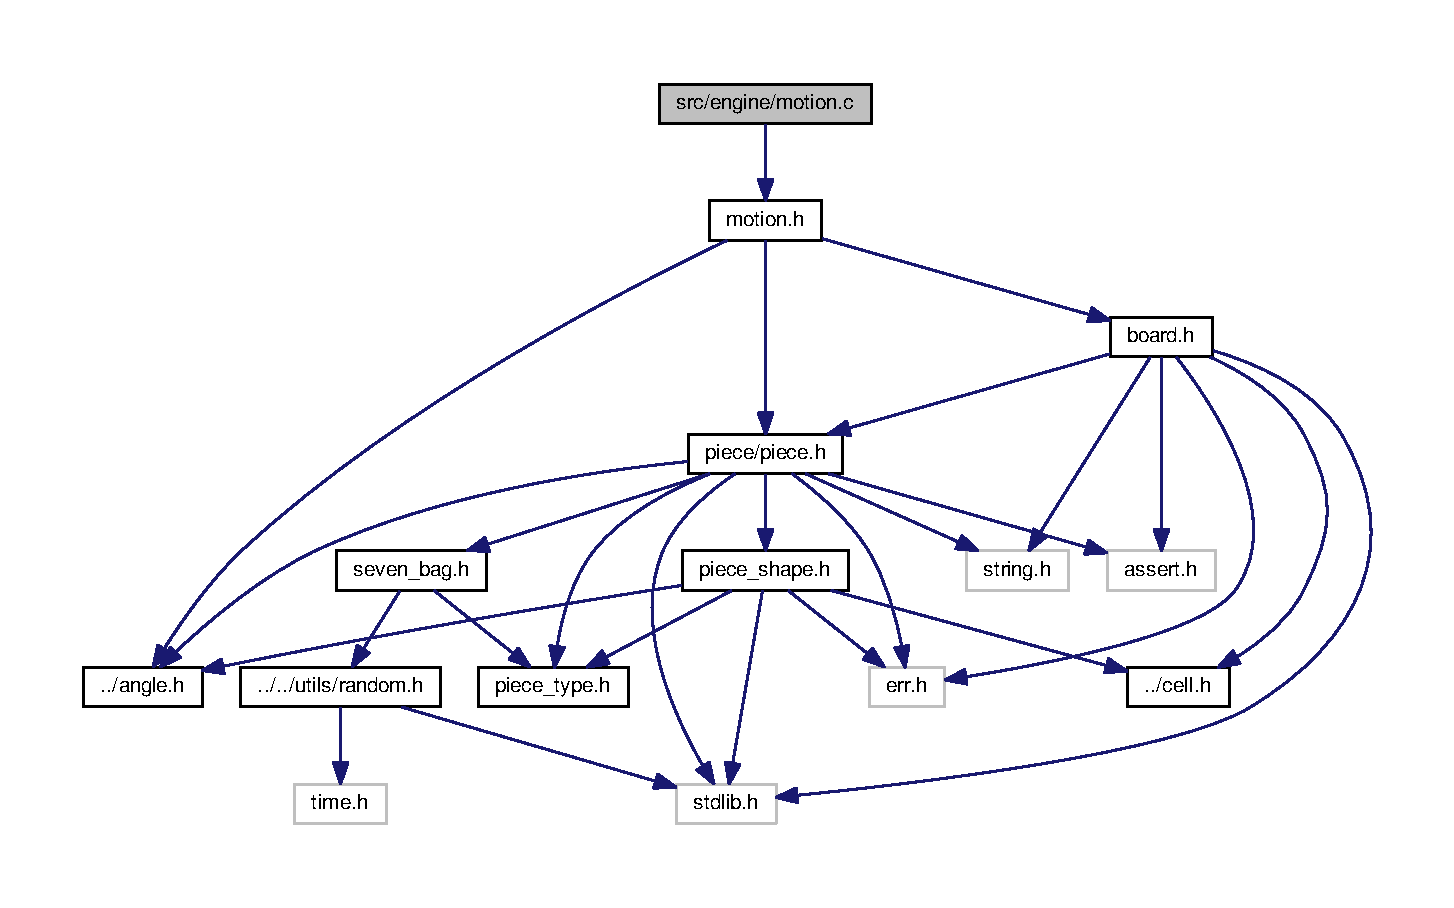
\includegraphics[width=350pt]{motion_8c__incl}
\end{center}
\end{figure}
\subsection*{Functions}
\begin{DoxyCompactItemize}
\item 
int \textbf{ motion\+\_\+can\+\_\+move} (struct \textbf{ piece} pc, const struct \textbf{ board} $\ast$brd, int dx, int dy)
\item 
int \textbf{ motion\+\_\+can\+\_\+rotate} (struct \textbf{ piece} pc, const struct \textbf{ board} $\ast$brd, int rotation)
\item 
int \textbf{ motion\+\_\+try\+\_\+move} (struct \textbf{ piece} $\ast$pc, const struct \textbf{ board} $\ast$brd, int dx, int dy)
\item 
int \textbf{ motion\+\_\+try\+\_\+rotate} (struct \textbf{ piece} $\ast$pc, const struct \textbf{ board} $\ast$brd, int rotation)
\item 
int \textbf{ motion\+\_\+try\+\_\+move\+\_\+down} (struct \textbf{ piece} $\ast$pc, const struct \textbf{ board} $\ast$brd)
\end{DoxyCompactItemize}


\subsection{Detailed Description}
No description. 

\begin{DoxyAuthor}{Author}
S4\+Master\+Race 
\end{DoxyAuthor}
\begin{DoxyVersion}{Version}
1.\+0 
\end{DoxyVersion}


\subsection{Function Documentation}
\mbox{\label{motion_8c_a44d62ec0304b3efce7d5d76f597fed22}} 
\index{motion.\+c@{motion.\+c}!motion\+\_\+can\+\_\+move@{motion\+\_\+can\+\_\+move}}
\index{motion\+\_\+can\+\_\+move@{motion\+\_\+can\+\_\+move}!motion.\+c@{motion.\+c}}
\subsubsection{motion\+\_\+can\+\_\+move()}
{\footnotesize\ttfamily int motion\+\_\+can\+\_\+move (\begin{DoxyParamCaption}\item[{struct \textbf{ piece}}]{pc,  }\item[{const struct \textbf{ board} $\ast$}]{brd,  }\item[{int}]{dx,  }\item[{int}]{dy }\end{DoxyParamCaption})}

\mbox{\label{motion_8c_afd171d9e0c9f0884598c492d7d3ed8e9}} 
\index{motion.\+c@{motion.\+c}!motion\+\_\+can\+\_\+rotate@{motion\+\_\+can\+\_\+rotate}}
\index{motion\+\_\+can\+\_\+rotate@{motion\+\_\+can\+\_\+rotate}!motion.\+c@{motion.\+c}}
\subsubsection{motion\+\_\+can\+\_\+rotate()}
{\footnotesize\ttfamily int motion\+\_\+can\+\_\+rotate (\begin{DoxyParamCaption}\item[{struct \textbf{ piece}}]{pc,  }\item[{const struct \textbf{ board} $\ast$}]{brd,  }\item[{int}]{rotation }\end{DoxyParamCaption})}

\mbox{\label{motion_8c_a29682f9162cac571bd205e47492c5ab8}} 
\index{motion.\+c@{motion.\+c}!motion\+\_\+try\+\_\+move@{motion\+\_\+try\+\_\+move}}
\index{motion\+\_\+try\+\_\+move@{motion\+\_\+try\+\_\+move}!motion.\+c@{motion.\+c}}
\subsubsection{motion\+\_\+try\+\_\+move()}
{\footnotesize\ttfamily int motion\+\_\+try\+\_\+move (\begin{DoxyParamCaption}\item[{struct \textbf{ piece} $\ast$}]{pc,  }\item[{const struct \textbf{ board} $\ast$}]{brd,  }\item[{int}]{dx,  }\item[{int}]{dy }\end{DoxyParamCaption})}

\mbox{\label{motion_8c_a416d5d5b14ef78b17dd4f892627556ac}} 
\index{motion.\+c@{motion.\+c}!motion\+\_\+try\+\_\+move\+\_\+down@{motion\+\_\+try\+\_\+move\+\_\+down}}
\index{motion\+\_\+try\+\_\+move\+\_\+down@{motion\+\_\+try\+\_\+move\+\_\+down}!motion.\+c@{motion.\+c}}
\subsubsection{motion\+\_\+try\+\_\+move\+\_\+down()}
{\footnotesize\ttfamily int motion\+\_\+try\+\_\+move\+\_\+down (\begin{DoxyParamCaption}\item[{struct \textbf{ piece} $\ast$}]{pc,  }\item[{const struct \textbf{ board} $\ast$}]{brd }\end{DoxyParamCaption})}

\mbox{\label{motion_8c_a249827f1bf1b0101949ba0818d13d8f5}} 
\index{motion.\+c@{motion.\+c}!motion\+\_\+try\+\_\+rotate@{motion\+\_\+try\+\_\+rotate}}
\index{motion\+\_\+try\+\_\+rotate@{motion\+\_\+try\+\_\+rotate}!motion.\+c@{motion.\+c}}
\subsubsection{motion\+\_\+try\+\_\+rotate()}
{\footnotesize\ttfamily int motion\+\_\+try\+\_\+rotate (\begin{DoxyParamCaption}\item[{struct \textbf{ piece} $\ast$}]{pc,  }\item[{const struct \textbf{ board} $\ast$}]{brd,  }\item[{int}]{rotation }\end{DoxyParamCaption})}


\section{src/engine/motion.h File Reference}
\label{motion_8h}\index{src/engine/motion.\+h@{src/engine/motion.\+h}}


Motion.  


{\ttfamily \#include \char`\"{}piece/piece.\+h\char`\"{}}\newline
{\ttfamily \#include \char`\"{}board.\+h\char`\"{}}\newline
{\ttfamily \#include \char`\"{}angle.\+h\char`\"{}}\newline
Include dependency graph for motion.\+h\+:
\nopagebreak
\begin{figure}[H]
\begin{center}
\leavevmode
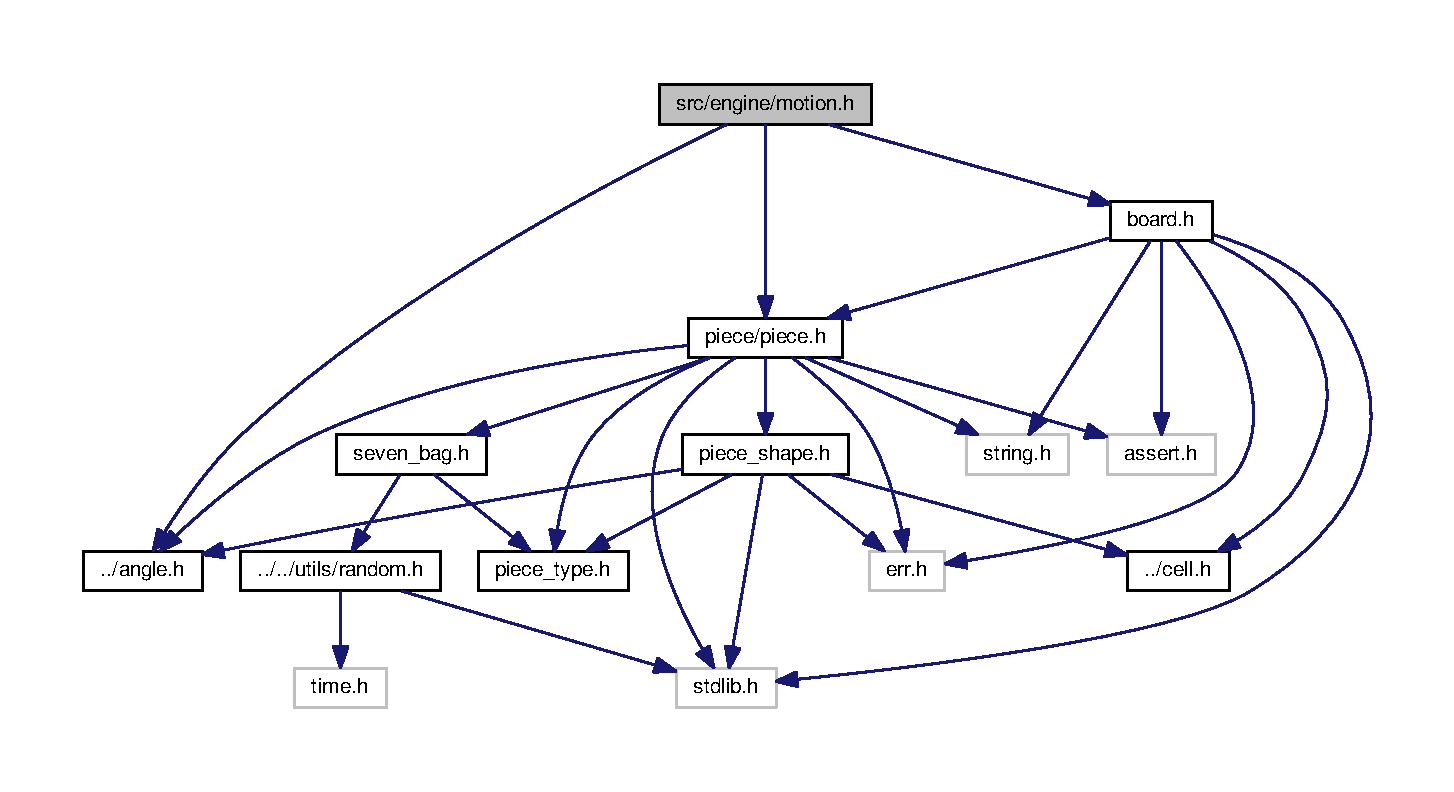
\includegraphics[width=350pt]{motion_8h__incl}
\end{center}
\end{figure}
This graph shows which files directly or indirectly include this file\+:
\nopagebreak
\begin{figure}[H]
\begin{center}
\leavevmode
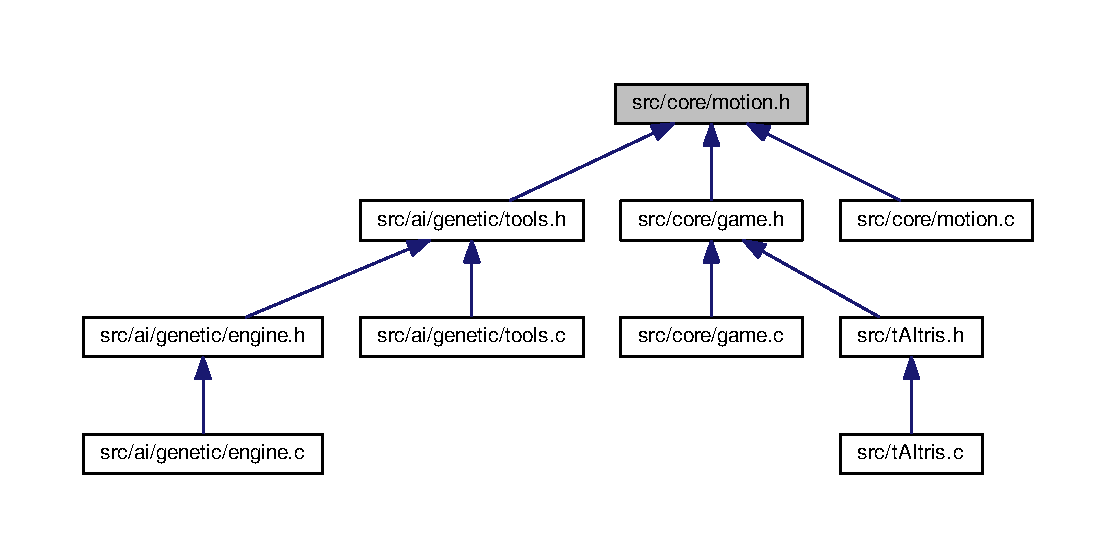
\includegraphics[width=350pt]{motion_8h__dep__incl}
\end{center}
\end{figure}
\subsection*{Functions}
\begin{DoxyCompactItemize}
\item 
int \textbf{ motion\+\_\+is\+\_\+valid} (const \textbf{ Piece} $\ast$pc, const \textbf{ Board} $\ast$brd)
\item 
int \textbf{ motion\+\_\+try\+\_\+move} (\textbf{ Piece} $\ast$pc, const \textbf{ Board} $\ast$brd, int dx, int dy)
\item 
int \textbf{ motion\+\_\+try\+\_\+rotate} (\textbf{ Piece} $\ast$pc, const \textbf{ Board} $\ast$brd, \textbf{ Rotation} r)
\item 
int \textbf{ motion\+\_\+try\+\_\+down} (\textbf{ Piece} $\ast$pc, const \textbf{ Board} $\ast$brd)
\item 
int \textbf{ motion\+\_\+can\+\_\+move} (const \textbf{ Piece} $\ast$pc, const \textbf{ Board} $\ast$brd, int dx, int dy)
\item 
int \textbf{ motion\+\_\+can\+\_\+rotate} (const \textbf{ Piece} $\ast$pc, const \textbf{ Board} $\ast$brd, \textbf{ Rotation} r)
\end{DoxyCompactItemize}


\subsection{Detailed Description}
Motion. 

\begin{DoxyAuthor}{Author}
S4\+Master\+Race 
\end{DoxyAuthor}
\begin{DoxyVersion}{Version}
2.\+0 
\end{DoxyVersion}


\subsection{Function Documentation}
\mbox{\label{motion_8h_ab199a2d7f6a562940345b4ec28e32ed2}} 
\index{motion.\+h@{motion.\+h}!motion\+\_\+can\+\_\+move@{motion\+\_\+can\+\_\+move}}
\index{motion\+\_\+can\+\_\+move@{motion\+\_\+can\+\_\+move}!motion.\+h@{motion.\+h}}
\subsubsection{motion\+\_\+can\+\_\+move()}
{\footnotesize\ttfamily int motion\+\_\+can\+\_\+move (\begin{DoxyParamCaption}\item[{const \textbf{ Piece} $\ast$}]{pc,  }\item[{const \textbf{ Board} $\ast$}]{brd,  }\item[{int}]{dx,  }\item[{int}]{dy }\end{DoxyParamCaption})}

\mbox{\label{motion_8h_ad3500291202fdc724ca7babd2df944ba}} 
\index{motion.\+h@{motion.\+h}!motion\+\_\+can\+\_\+rotate@{motion\+\_\+can\+\_\+rotate}}
\index{motion\+\_\+can\+\_\+rotate@{motion\+\_\+can\+\_\+rotate}!motion.\+h@{motion.\+h}}
\subsubsection{motion\+\_\+can\+\_\+rotate()}
{\footnotesize\ttfamily int motion\+\_\+can\+\_\+rotate (\begin{DoxyParamCaption}\item[{const \textbf{ Piece} $\ast$}]{pc,  }\item[{const \textbf{ Board} $\ast$}]{brd,  }\item[{\textbf{ Rotation}}]{r }\end{DoxyParamCaption})}

\mbox{\label{motion_8h_ae67cef6a127c61180c181edb84120ef9}} 
\index{motion.\+h@{motion.\+h}!motion\+\_\+is\+\_\+valid@{motion\+\_\+is\+\_\+valid}}
\index{motion\+\_\+is\+\_\+valid@{motion\+\_\+is\+\_\+valid}!motion.\+h@{motion.\+h}}
\subsubsection{motion\+\_\+is\+\_\+valid()}
{\footnotesize\ttfamily int motion\+\_\+is\+\_\+valid (\begin{DoxyParamCaption}\item[{const \textbf{ Piece} $\ast$}]{pc,  }\item[{const \textbf{ Board} $\ast$}]{brd }\end{DoxyParamCaption})}

\mbox{\label{motion_8h_af0d588d036f656d0f629b8115b45df60}} 
\index{motion.\+h@{motion.\+h}!motion\+\_\+try\+\_\+down@{motion\+\_\+try\+\_\+down}}
\index{motion\+\_\+try\+\_\+down@{motion\+\_\+try\+\_\+down}!motion.\+h@{motion.\+h}}
\subsubsection{motion\+\_\+try\+\_\+down()}
{\footnotesize\ttfamily int motion\+\_\+try\+\_\+down (\begin{DoxyParamCaption}\item[{\textbf{ Piece} $\ast$}]{pc,  }\item[{const \textbf{ Board} $\ast$}]{brd }\end{DoxyParamCaption})}

\mbox{\label{motion_8h_a2cf016bccf6ca6fa09a3cb5362fbd6b7}} 
\index{motion.\+h@{motion.\+h}!motion\+\_\+try\+\_\+move@{motion\+\_\+try\+\_\+move}}
\index{motion\+\_\+try\+\_\+move@{motion\+\_\+try\+\_\+move}!motion.\+h@{motion.\+h}}
\subsubsection{motion\+\_\+try\+\_\+move()}
{\footnotesize\ttfamily int motion\+\_\+try\+\_\+move (\begin{DoxyParamCaption}\item[{\textbf{ Piece} $\ast$}]{pc,  }\item[{const \textbf{ Board} $\ast$}]{brd,  }\item[{int}]{dx,  }\item[{int}]{dy }\end{DoxyParamCaption})}

\mbox{\label{motion_8h_a89a0f1321575d3346ebd65f5e2953d71}} 
\index{motion.\+h@{motion.\+h}!motion\+\_\+try\+\_\+rotate@{motion\+\_\+try\+\_\+rotate}}
\index{motion\+\_\+try\+\_\+rotate@{motion\+\_\+try\+\_\+rotate}!motion.\+h@{motion.\+h}}
\subsubsection{motion\+\_\+try\+\_\+rotate()}
{\footnotesize\ttfamily int motion\+\_\+try\+\_\+rotate (\begin{DoxyParamCaption}\item[{\textbf{ Piece} $\ast$}]{pc,  }\item[{const \textbf{ Board} $\ast$}]{brd,  }\item[{\textbf{ Rotation}}]{r }\end{DoxyParamCaption})}


\section{src/core/piece.c File Reference}
\label{piece_8c}\index{src/core/piece.\+c@{src/core/piece.\+c}}


No description.  


{\ttfamily \#include \char`\"{}piece.\+h\char`\"{}}\newline
Include dependency graph for piece.\+c\+:
\nopagebreak
\begin{figure}[H]
\begin{center}
\leavevmode
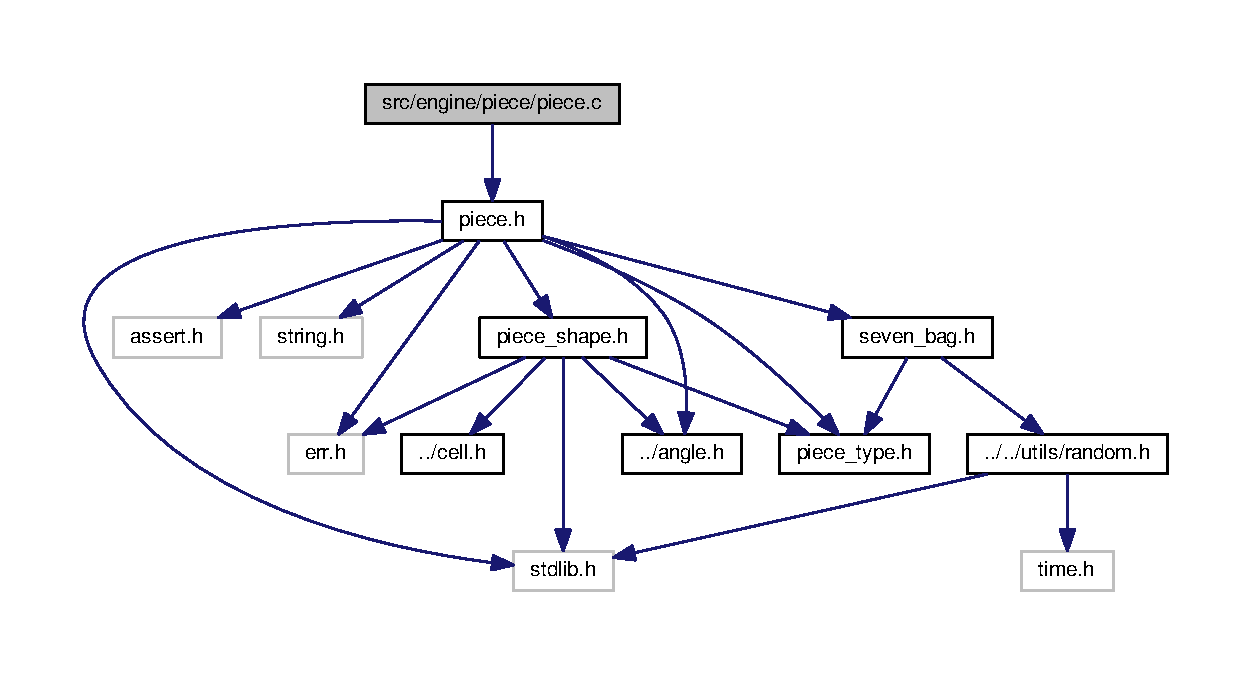
\includegraphics[width=317pt]{piece_8c__incl}
\end{center}
\end{figure}
\subsection*{Functions}
\begin{DoxyCompactItemize}
\item 
void \textbf{ piece\+\_\+random} (struct \textbf{ piece} $\ast$pc, size\+\_\+t x, size\+\_\+t y)
\item 
void \textbf{ piece\+\_\+move} (struct \textbf{ piece} $\ast$pc, int dx, int dy)
\item 
void \textbf{ piece\+\_\+rotate} (struct \textbf{ piece} $\ast$pc, int rotation)
\end{DoxyCompactItemize}
\subsection*{Variables}
\begin{DoxyCompactItemize}
\item 
const int \textbf{ P\+I\+E\+C\+E\+\_\+\+S\+H\+A\+P\+ES} [7][4][4][4]
\end{DoxyCompactItemize}


\subsection{Detailed Description}
No description. 

\begin{DoxyAuthor}{Author}
S4\+Master\+Race 
\end{DoxyAuthor}
\begin{DoxyVersion}{Version}
1.\+0 
\end{DoxyVersion}


\subsection{Function Documentation}
\mbox{\label{piece_8c_a4642eff00c1b15fd507057c44e6736a0}} 
\index{piece.\+c@{piece.\+c}!piece\+\_\+move@{piece\+\_\+move}}
\index{piece\+\_\+move@{piece\+\_\+move}!piece.\+c@{piece.\+c}}
\subsubsection{piece\+\_\+move()}
{\footnotesize\ttfamily void piece\+\_\+move (\begin{DoxyParamCaption}\item[{struct \textbf{ piece} $\ast$}]{pc,  }\item[{int}]{dx,  }\item[{int}]{dy }\end{DoxyParamCaption})\hspace{0.3cm}{\ttfamily [inline]}}

\mbox{\label{piece_8c_af5ed528ee08179282cc95a5431aba453}} 
\index{piece.\+c@{piece.\+c}!piece\+\_\+random@{piece\+\_\+random}}
\index{piece\+\_\+random@{piece\+\_\+random}!piece.\+c@{piece.\+c}}
\subsubsection{piece\+\_\+random()}
{\footnotesize\ttfamily void piece\+\_\+random (\begin{DoxyParamCaption}\item[{struct \textbf{ piece} $\ast$}]{pc,  }\item[{size\+\_\+t}]{x,  }\item[{size\+\_\+t}]{y }\end{DoxyParamCaption})\hspace{0.3cm}{\ttfamily [inline]}}

\mbox{\label{piece_8c_af73ec0a224e50fee25089a256145bbd2}} 
\index{piece.\+c@{piece.\+c}!piece\+\_\+rotate@{piece\+\_\+rotate}}
\index{piece\+\_\+rotate@{piece\+\_\+rotate}!piece.\+c@{piece.\+c}}
\subsubsection{piece\+\_\+rotate()}
{\footnotesize\ttfamily void piece\+\_\+rotate (\begin{DoxyParamCaption}\item[{struct \textbf{ piece} $\ast$}]{pc,  }\item[{int}]{rotation }\end{DoxyParamCaption})\hspace{0.3cm}{\ttfamily [inline]}}



\subsection{Variable Documentation}
\mbox{\label{piece_8c_aa012dcbe0482f140b29dcdd7e252ebeb}} 
\index{piece.\+c@{piece.\+c}!P\+I\+E\+C\+E\+\_\+\+S\+H\+A\+P\+ES@{P\+I\+E\+C\+E\+\_\+\+S\+H\+A\+P\+ES}}
\index{P\+I\+E\+C\+E\+\_\+\+S\+H\+A\+P\+ES@{P\+I\+E\+C\+E\+\_\+\+S\+H\+A\+P\+ES}!piece.\+c@{piece.\+c}}
\subsubsection{P\+I\+E\+C\+E\+\_\+\+S\+H\+A\+P\+ES}
{\footnotesize\ttfamily const int P\+I\+E\+C\+E\+\_\+\+S\+H\+A\+P\+ES[7][4][4][4]}


\section{src/core/piece.h File Reference}
\label{piece_8h}\index{src/core/piece.\+h@{src/core/piece.\+h}}


No description.  


{\ttfamily \#include $<$stdlib.\+h$>$}\newline
{\ttfamily \#include $<$assert.\+h$>$}\newline
{\ttfamily \#include $<$string.\+h$>$}\newline
{\ttfamily \#include \char`\"{}../utils/random.\+h\char`\"{}}\newline
Include dependency graph for piece.\+h\+:
\nopagebreak
\begin{figure}[H]
\begin{center}
\leavevmode
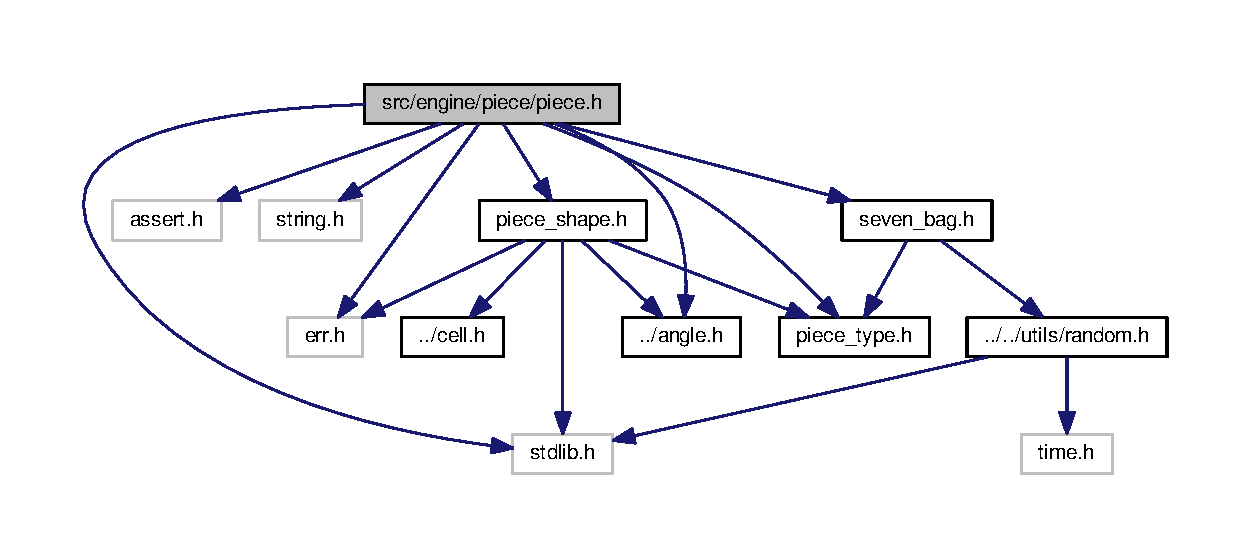
\includegraphics[width=317pt]{piece_8h__incl}
\end{center}
\end{figure}
This graph shows which files directly or indirectly include this file\+:
\nopagebreak
\begin{figure}[H]
\begin{center}
\leavevmode
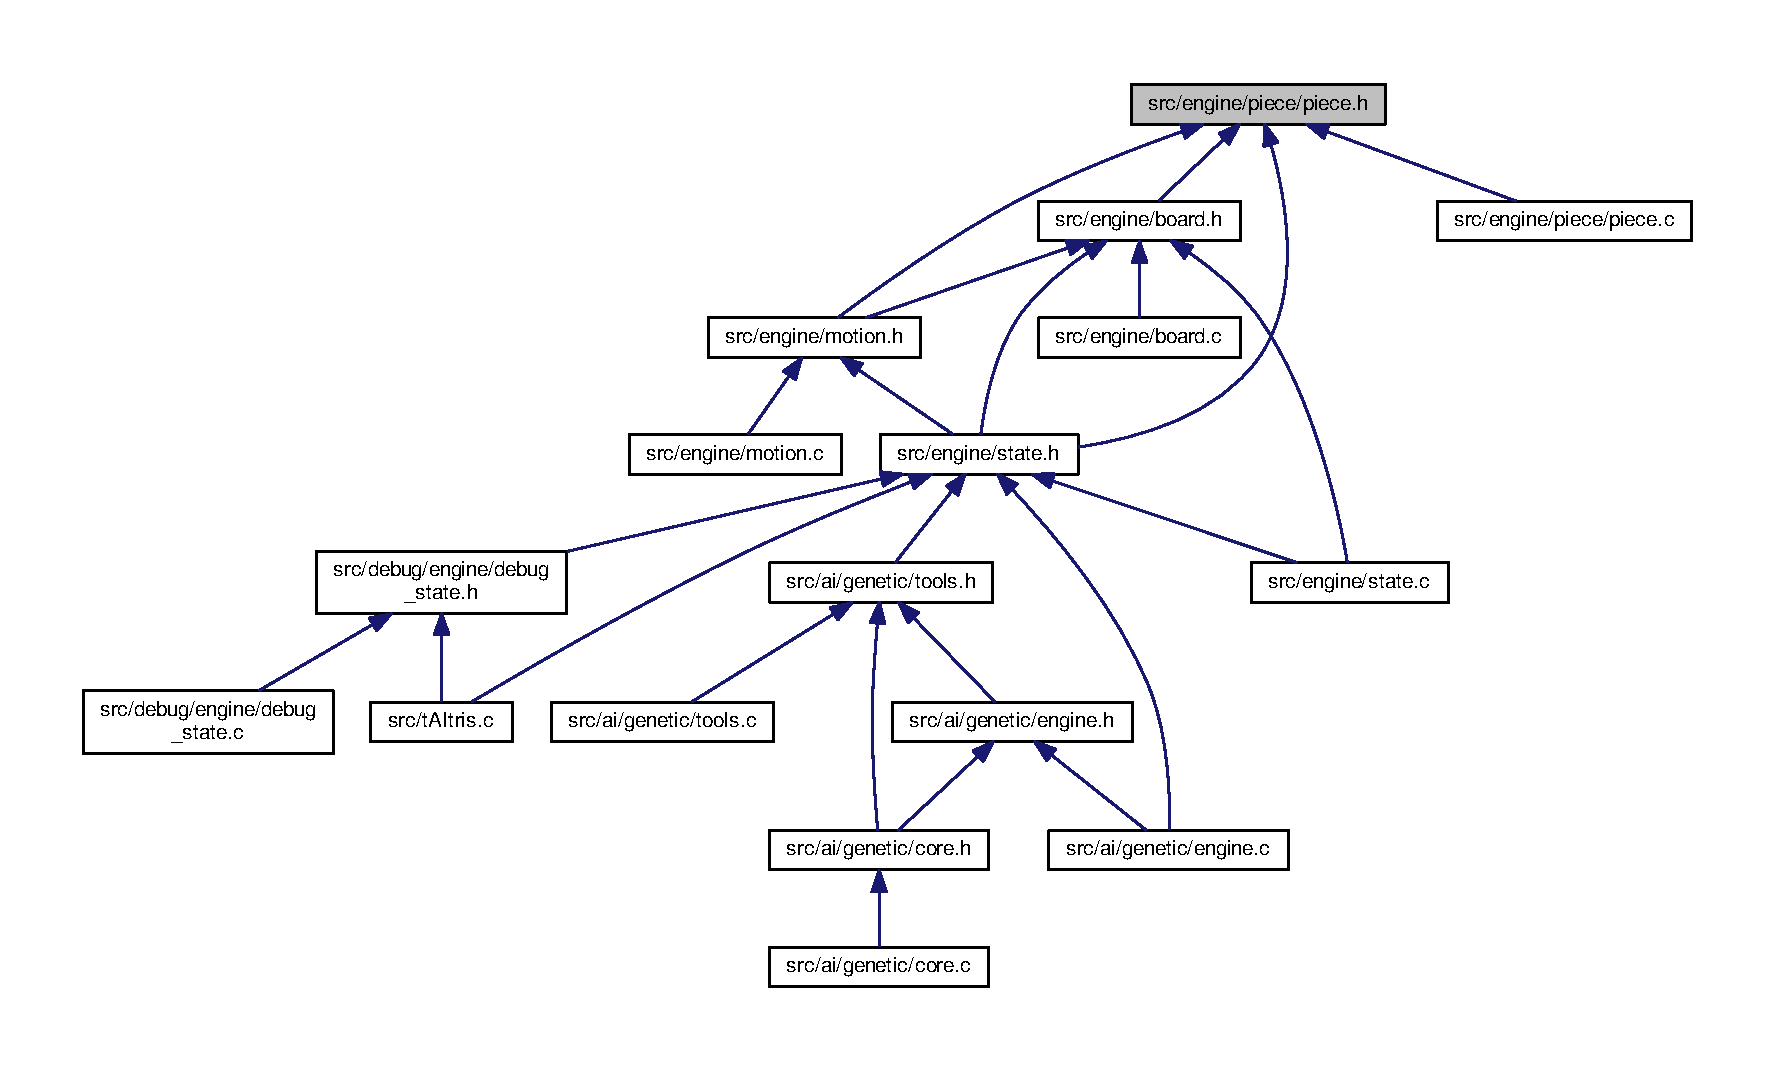
\includegraphics[width=350pt]{piece_8h__dep__incl}
\end{center}
\end{figure}
\subsection*{Data Structures}
\begin{DoxyCompactItemize}
\item 
struct \textbf{ piece}
\end{DoxyCompactItemize}
\subsection*{Macros}
\begin{DoxyCompactItemize}
\item 
\#define \textbf{ P\+I\+E\+C\+E\+\_\+I}~0
\item 
\#define \textbf{ P\+I\+E\+C\+E\+\_\+O}~1
\item 
\#define \textbf{ P\+I\+E\+C\+E\+\_\+T}~2
\item 
\#define \textbf{ P\+I\+E\+C\+E\+\_\+L}~3
\item 
\#define \textbf{ P\+I\+E\+C\+E\+\_\+J}~4
\item 
\#define \textbf{ P\+I\+E\+C\+E\+\_\+Z}~5
\item 
\#define \textbf{ P\+I\+E\+C\+E\+\_\+S}~6
\item 
\#define \textbf{ P\+I\+E\+C\+E\+\_\+\+C\+O\+U\+NT}~7
\item 
\#define \textbf{ P\+I\+E\+C\+E\+\_\+\+W\+I\+D\+TH}~4
\item 
\#define \textbf{ P\+I\+E\+C\+E\+\_\+\+H\+E\+I\+G\+HT}~4
\item 
\#define \textbf{ P\+I\+E\+C\+E\+\_\+\+A\+N\+G\+L\+E\+\_\+\+UP}~0
\item 
\#define \textbf{ P\+I\+E\+C\+E\+\_\+\+A\+N\+G\+L\+E\+\_\+\+R\+I\+G\+HT}~1
\item 
\#define \textbf{ P\+I\+E\+C\+E\+\_\+\+A\+N\+G\+L\+E\+\_\+\+D\+O\+WN}~2
\item 
\#define \textbf{ P\+I\+E\+C\+E\+\_\+\+A\+N\+G\+L\+E\+\_\+\+L\+E\+FT}~3
\item 
\#define \textbf{ P\+I\+E\+C\+E\+\_\+\+A\+N\+G\+L\+ES}~4
\item 
\#define \textbf{ P\+I\+E\+C\+E\+\_\+\+R\+O\+T\+A\+T\+E\+\_\+\+L\+E\+FT}~(-\/1)
\item 
\#define \textbf{ P\+I\+E\+C\+E\+\_\+\+R\+O\+T\+A\+T\+E\+\_\+\+R\+I\+G\+HT}~1
\end{DoxyCompactItemize}
\subsection*{Functions}
\begin{DoxyCompactItemize}
\item 
void \textbf{ piece\+\_\+random} (struct \textbf{ piece} $\ast$pc, size\+\_\+t x, size\+\_\+t y)
\item 
void \textbf{ piece\+\_\+move} (struct \textbf{ piece} $\ast$pc, int dx, int dy)
\item 
void \textbf{ piece\+\_\+rotate} (struct \textbf{ piece} $\ast$pc, int rotation)
\end{DoxyCompactItemize}
\subsection*{Variables}
\begin{DoxyCompactItemize}
\item 
const int \textbf{ P\+I\+E\+C\+E\+\_\+\+S\+H\+A\+P\+ES} [\textbf{ P\+I\+E\+C\+E\+\_\+\+C\+O\+U\+NT}][\textbf{ P\+I\+E\+C\+E\+\_\+\+A\+N\+G\+L\+ES}][\textbf{ P\+I\+E\+C\+E\+\_\+\+H\+E\+I\+G\+HT}][\textbf{ P\+I\+E\+C\+E\+\_\+\+W\+I\+D\+TH}]
\end{DoxyCompactItemize}


\subsection{Detailed Description}
No description. 

\begin{DoxyAuthor}{Author}
S4\+Master\+Race 
\end{DoxyAuthor}
\begin{DoxyVersion}{Version}
1.\+0 
\end{DoxyVersion}


\subsection{Macro Definition Documentation}
\mbox{\label{piece_8h_a7651297f25bb454ba6381e1c2f0ec04a}} 
\index{piece.\+h@{piece.\+h}!P\+I\+E\+C\+E\+\_\+\+A\+N\+G\+L\+E\+\_\+\+D\+O\+WN@{P\+I\+E\+C\+E\+\_\+\+A\+N\+G\+L\+E\+\_\+\+D\+O\+WN}}
\index{P\+I\+E\+C\+E\+\_\+\+A\+N\+G\+L\+E\+\_\+\+D\+O\+WN@{P\+I\+E\+C\+E\+\_\+\+A\+N\+G\+L\+E\+\_\+\+D\+O\+WN}!piece.\+h@{piece.\+h}}
\subsubsection{P\+I\+E\+C\+E\+\_\+\+A\+N\+G\+L\+E\+\_\+\+D\+O\+WN}
{\footnotesize\ttfamily \#define P\+I\+E\+C\+E\+\_\+\+A\+N\+G\+L\+E\+\_\+\+D\+O\+WN~2}

\mbox{\label{piece_8h_ad25a993e90f645aa7d7651adf650e51d}} 
\index{piece.\+h@{piece.\+h}!P\+I\+E\+C\+E\+\_\+\+A\+N\+G\+L\+E\+\_\+\+L\+E\+FT@{P\+I\+E\+C\+E\+\_\+\+A\+N\+G\+L\+E\+\_\+\+L\+E\+FT}}
\index{P\+I\+E\+C\+E\+\_\+\+A\+N\+G\+L\+E\+\_\+\+L\+E\+FT@{P\+I\+E\+C\+E\+\_\+\+A\+N\+G\+L\+E\+\_\+\+L\+E\+FT}!piece.\+h@{piece.\+h}}
\subsubsection{P\+I\+E\+C\+E\+\_\+\+A\+N\+G\+L\+E\+\_\+\+L\+E\+FT}
{\footnotesize\ttfamily \#define P\+I\+E\+C\+E\+\_\+\+A\+N\+G\+L\+E\+\_\+\+L\+E\+FT~3}

\mbox{\label{piece_8h_abf98bf1ad32ce58c5fa85df607e35407}} 
\index{piece.\+h@{piece.\+h}!P\+I\+E\+C\+E\+\_\+\+A\+N\+G\+L\+E\+\_\+\+R\+I\+G\+HT@{P\+I\+E\+C\+E\+\_\+\+A\+N\+G\+L\+E\+\_\+\+R\+I\+G\+HT}}
\index{P\+I\+E\+C\+E\+\_\+\+A\+N\+G\+L\+E\+\_\+\+R\+I\+G\+HT@{P\+I\+E\+C\+E\+\_\+\+A\+N\+G\+L\+E\+\_\+\+R\+I\+G\+HT}!piece.\+h@{piece.\+h}}
\subsubsection{P\+I\+E\+C\+E\+\_\+\+A\+N\+G\+L\+E\+\_\+\+R\+I\+G\+HT}
{\footnotesize\ttfamily \#define P\+I\+E\+C\+E\+\_\+\+A\+N\+G\+L\+E\+\_\+\+R\+I\+G\+HT~1}

\mbox{\label{piece_8h_a7452501247a73a9decd4a021ee8030b2}} 
\index{piece.\+h@{piece.\+h}!P\+I\+E\+C\+E\+\_\+\+A\+N\+G\+L\+E\+\_\+\+UP@{P\+I\+E\+C\+E\+\_\+\+A\+N\+G\+L\+E\+\_\+\+UP}}
\index{P\+I\+E\+C\+E\+\_\+\+A\+N\+G\+L\+E\+\_\+\+UP@{P\+I\+E\+C\+E\+\_\+\+A\+N\+G\+L\+E\+\_\+\+UP}!piece.\+h@{piece.\+h}}
\subsubsection{P\+I\+E\+C\+E\+\_\+\+A\+N\+G\+L\+E\+\_\+\+UP}
{\footnotesize\ttfamily \#define P\+I\+E\+C\+E\+\_\+\+A\+N\+G\+L\+E\+\_\+\+UP~0}

\mbox{\label{piece_8h_a45d1e9768cbb0fe160fb97b7f47e3347}} 
\index{piece.\+h@{piece.\+h}!P\+I\+E\+C\+E\+\_\+\+A\+N\+G\+L\+ES@{P\+I\+E\+C\+E\+\_\+\+A\+N\+G\+L\+ES}}
\index{P\+I\+E\+C\+E\+\_\+\+A\+N\+G\+L\+ES@{P\+I\+E\+C\+E\+\_\+\+A\+N\+G\+L\+ES}!piece.\+h@{piece.\+h}}
\subsubsection{P\+I\+E\+C\+E\+\_\+\+A\+N\+G\+L\+ES}
{\footnotesize\ttfamily \#define P\+I\+E\+C\+E\+\_\+\+A\+N\+G\+L\+ES~4}

\mbox{\label{piece_8h_a5b9184bdc00e9c9ab6594aea6ea35112}} 
\index{piece.\+h@{piece.\+h}!P\+I\+E\+C\+E\+\_\+\+C\+O\+U\+NT@{P\+I\+E\+C\+E\+\_\+\+C\+O\+U\+NT}}
\index{P\+I\+E\+C\+E\+\_\+\+C\+O\+U\+NT@{P\+I\+E\+C\+E\+\_\+\+C\+O\+U\+NT}!piece.\+h@{piece.\+h}}
\subsubsection{P\+I\+E\+C\+E\+\_\+\+C\+O\+U\+NT}
{\footnotesize\ttfamily \#define P\+I\+E\+C\+E\+\_\+\+C\+O\+U\+NT~7}

\mbox{\label{piece_8h_ad8eac8f6a24533f84ba2be5fbefa1644}} 
\index{piece.\+h@{piece.\+h}!P\+I\+E\+C\+E\+\_\+\+H\+E\+I\+G\+HT@{P\+I\+E\+C\+E\+\_\+\+H\+E\+I\+G\+HT}}
\index{P\+I\+E\+C\+E\+\_\+\+H\+E\+I\+G\+HT@{P\+I\+E\+C\+E\+\_\+\+H\+E\+I\+G\+HT}!piece.\+h@{piece.\+h}}
\subsubsection{P\+I\+E\+C\+E\+\_\+\+H\+E\+I\+G\+HT}
{\footnotesize\ttfamily \#define P\+I\+E\+C\+E\+\_\+\+H\+E\+I\+G\+HT~4}

\mbox{\label{piece_8h_a91f2021e61458e0777dab6373eedd60b}} 
\index{piece.\+h@{piece.\+h}!P\+I\+E\+C\+E\+\_\+I@{P\+I\+E\+C\+E\+\_\+I}}
\index{P\+I\+E\+C\+E\+\_\+I@{P\+I\+E\+C\+E\+\_\+I}!piece.\+h@{piece.\+h}}
\subsubsection{P\+I\+E\+C\+E\+\_\+I}
{\footnotesize\ttfamily \#define P\+I\+E\+C\+E\+\_\+I~0}

\mbox{\label{piece_8h_afeee888737fee08d7151943e80de0a15}} 
\index{piece.\+h@{piece.\+h}!P\+I\+E\+C\+E\+\_\+J@{P\+I\+E\+C\+E\+\_\+J}}
\index{P\+I\+E\+C\+E\+\_\+J@{P\+I\+E\+C\+E\+\_\+J}!piece.\+h@{piece.\+h}}
\subsubsection{P\+I\+E\+C\+E\+\_\+J}
{\footnotesize\ttfamily \#define P\+I\+E\+C\+E\+\_\+J~4}

\mbox{\label{piece_8h_ad29ec00683ddc760a084b83009b3160c}} 
\index{piece.\+h@{piece.\+h}!P\+I\+E\+C\+E\+\_\+L@{P\+I\+E\+C\+E\+\_\+L}}
\index{P\+I\+E\+C\+E\+\_\+L@{P\+I\+E\+C\+E\+\_\+L}!piece.\+h@{piece.\+h}}
\subsubsection{P\+I\+E\+C\+E\+\_\+L}
{\footnotesize\ttfamily \#define P\+I\+E\+C\+E\+\_\+L~3}

\mbox{\label{piece_8h_a35b88195092e30210aba2f4d646f3a9c}} 
\index{piece.\+h@{piece.\+h}!P\+I\+E\+C\+E\+\_\+O@{P\+I\+E\+C\+E\+\_\+O}}
\index{P\+I\+E\+C\+E\+\_\+O@{P\+I\+E\+C\+E\+\_\+O}!piece.\+h@{piece.\+h}}
\subsubsection{P\+I\+E\+C\+E\+\_\+O}
{\footnotesize\ttfamily \#define P\+I\+E\+C\+E\+\_\+O~1}

\mbox{\label{piece_8h_a525f44cc5c3e7c3cfc846364b2983575}} 
\index{piece.\+h@{piece.\+h}!P\+I\+E\+C\+E\+\_\+\+R\+O\+T\+A\+T\+E\+\_\+\+L\+E\+FT@{P\+I\+E\+C\+E\+\_\+\+R\+O\+T\+A\+T\+E\+\_\+\+L\+E\+FT}}
\index{P\+I\+E\+C\+E\+\_\+\+R\+O\+T\+A\+T\+E\+\_\+\+L\+E\+FT@{P\+I\+E\+C\+E\+\_\+\+R\+O\+T\+A\+T\+E\+\_\+\+L\+E\+FT}!piece.\+h@{piece.\+h}}
\subsubsection{P\+I\+E\+C\+E\+\_\+\+R\+O\+T\+A\+T\+E\+\_\+\+L\+E\+FT}
{\footnotesize\ttfamily \#define P\+I\+E\+C\+E\+\_\+\+R\+O\+T\+A\+T\+E\+\_\+\+L\+E\+FT~(-\/1)}

\mbox{\label{piece_8h_a96616e68596e842766c50155546ccfd6}} 
\index{piece.\+h@{piece.\+h}!P\+I\+E\+C\+E\+\_\+\+R\+O\+T\+A\+T\+E\+\_\+\+R\+I\+G\+HT@{P\+I\+E\+C\+E\+\_\+\+R\+O\+T\+A\+T\+E\+\_\+\+R\+I\+G\+HT}}
\index{P\+I\+E\+C\+E\+\_\+\+R\+O\+T\+A\+T\+E\+\_\+\+R\+I\+G\+HT@{P\+I\+E\+C\+E\+\_\+\+R\+O\+T\+A\+T\+E\+\_\+\+R\+I\+G\+HT}!piece.\+h@{piece.\+h}}
\subsubsection{P\+I\+E\+C\+E\+\_\+\+R\+O\+T\+A\+T\+E\+\_\+\+R\+I\+G\+HT}
{\footnotesize\ttfamily \#define P\+I\+E\+C\+E\+\_\+\+R\+O\+T\+A\+T\+E\+\_\+\+R\+I\+G\+HT~1}

\mbox{\label{piece_8h_ad279ae03554c3ed297ec003495db1e2b}} 
\index{piece.\+h@{piece.\+h}!P\+I\+E\+C\+E\+\_\+S@{P\+I\+E\+C\+E\+\_\+S}}
\index{P\+I\+E\+C\+E\+\_\+S@{P\+I\+E\+C\+E\+\_\+S}!piece.\+h@{piece.\+h}}
\subsubsection{P\+I\+E\+C\+E\+\_\+S}
{\footnotesize\ttfamily \#define P\+I\+E\+C\+E\+\_\+S~6}

\mbox{\label{piece_8h_a2a6cc746fc6654970a62559f1d77a962}} 
\index{piece.\+h@{piece.\+h}!P\+I\+E\+C\+E\+\_\+T@{P\+I\+E\+C\+E\+\_\+T}}
\index{P\+I\+E\+C\+E\+\_\+T@{P\+I\+E\+C\+E\+\_\+T}!piece.\+h@{piece.\+h}}
\subsubsection{P\+I\+E\+C\+E\+\_\+T}
{\footnotesize\ttfamily \#define P\+I\+E\+C\+E\+\_\+T~2}

\mbox{\label{piece_8h_a3133e70647d4ab89f00ebb455ad964b8}} 
\index{piece.\+h@{piece.\+h}!P\+I\+E\+C\+E\+\_\+\+W\+I\+D\+TH@{P\+I\+E\+C\+E\+\_\+\+W\+I\+D\+TH}}
\index{P\+I\+E\+C\+E\+\_\+\+W\+I\+D\+TH@{P\+I\+E\+C\+E\+\_\+\+W\+I\+D\+TH}!piece.\+h@{piece.\+h}}
\subsubsection{P\+I\+E\+C\+E\+\_\+\+W\+I\+D\+TH}
{\footnotesize\ttfamily \#define P\+I\+E\+C\+E\+\_\+\+W\+I\+D\+TH~4}

\mbox{\label{piece_8h_aee707398916fd4752f85e771787c023c}} 
\index{piece.\+h@{piece.\+h}!P\+I\+E\+C\+E\+\_\+Z@{P\+I\+E\+C\+E\+\_\+Z}}
\index{P\+I\+E\+C\+E\+\_\+Z@{P\+I\+E\+C\+E\+\_\+Z}!piece.\+h@{piece.\+h}}
\subsubsection{P\+I\+E\+C\+E\+\_\+Z}
{\footnotesize\ttfamily \#define P\+I\+E\+C\+E\+\_\+Z~5}



\subsection{Function Documentation}
\mbox{\label{piece_8h_a4642eff00c1b15fd507057c44e6736a0}} 
\index{piece.\+h@{piece.\+h}!piece\+\_\+move@{piece\+\_\+move}}
\index{piece\+\_\+move@{piece\+\_\+move}!piece.\+h@{piece.\+h}}
\subsubsection{piece\+\_\+move()}
{\footnotesize\ttfamily void piece\+\_\+move (\begin{DoxyParamCaption}\item[{struct \textbf{ piece} $\ast$}]{pc,  }\item[{int}]{dx,  }\item[{int}]{dy }\end{DoxyParamCaption})\hspace{0.3cm}{\ttfamily [inline]}}

\mbox{\label{piece_8h_af5ed528ee08179282cc95a5431aba453}} 
\index{piece.\+h@{piece.\+h}!piece\+\_\+random@{piece\+\_\+random}}
\index{piece\+\_\+random@{piece\+\_\+random}!piece.\+h@{piece.\+h}}
\subsubsection{piece\+\_\+random()}
{\footnotesize\ttfamily void piece\+\_\+random (\begin{DoxyParamCaption}\item[{struct \textbf{ piece} $\ast$}]{pc,  }\item[{size\+\_\+t}]{x,  }\item[{size\+\_\+t}]{y }\end{DoxyParamCaption})\hspace{0.3cm}{\ttfamily [inline]}}

\mbox{\label{piece_8h_af73ec0a224e50fee25089a256145bbd2}} 
\index{piece.\+h@{piece.\+h}!piece\+\_\+rotate@{piece\+\_\+rotate}}
\index{piece\+\_\+rotate@{piece\+\_\+rotate}!piece.\+h@{piece.\+h}}
\subsubsection{piece\+\_\+rotate()}
{\footnotesize\ttfamily void piece\+\_\+rotate (\begin{DoxyParamCaption}\item[{struct \textbf{ piece} $\ast$}]{pc,  }\item[{int}]{rotation }\end{DoxyParamCaption})\hspace{0.3cm}{\ttfamily [inline]}}



\subsection{Variable Documentation}
\mbox{\label{piece_8h_a04d86212c54927c5c8e728121c430fde}} 
\index{piece.\+h@{piece.\+h}!P\+I\+E\+C\+E\+\_\+\+S\+H\+A\+P\+ES@{P\+I\+E\+C\+E\+\_\+\+S\+H\+A\+P\+ES}}
\index{P\+I\+E\+C\+E\+\_\+\+S\+H\+A\+P\+ES@{P\+I\+E\+C\+E\+\_\+\+S\+H\+A\+P\+ES}!piece.\+h@{piece.\+h}}
\subsubsection{P\+I\+E\+C\+E\+\_\+\+S\+H\+A\+P\+ES}
{\footnotesize\ttfamily const int P\+I\+E\+C\+E\+\_\+\+S\+H\+A\+P\+ES[\textbf{ P\+I\+E\+C\+E\+\_\+\+C\+O\+U\+NT}][\textbf{ P\+I\+E\+C\+E\+\_\+\+A\+N\+G\+L\+ES}][\textbf{ P\+I\+E\+C\+E\+\_\+\+H\+E\+I\+G\+HT}][\textbf{ P\+I\+E\+C\+E\+\_\+\+W\+I\+D\+TH}]}


\section{src/engine/piece/piece\+\_\+queue.c File Reference}
\label{piece__queue_8c}\index{src/engine/piece/piece\+\_\+queue.\+c@{src/engine/piece/piece\+\_\+queue.\+c}}


\doxyref{Piece}{p.}{structPiece} queue.  


{\ttfamily \#include \char`\"{}piece\+\_\+queue.\+h\char`\"{}}\newline
Include dependency graph for piece\+\_\+queue.\+c\+:
\nopagebreak
\begin{figure}[H]
\begin{center}
\leavevmode
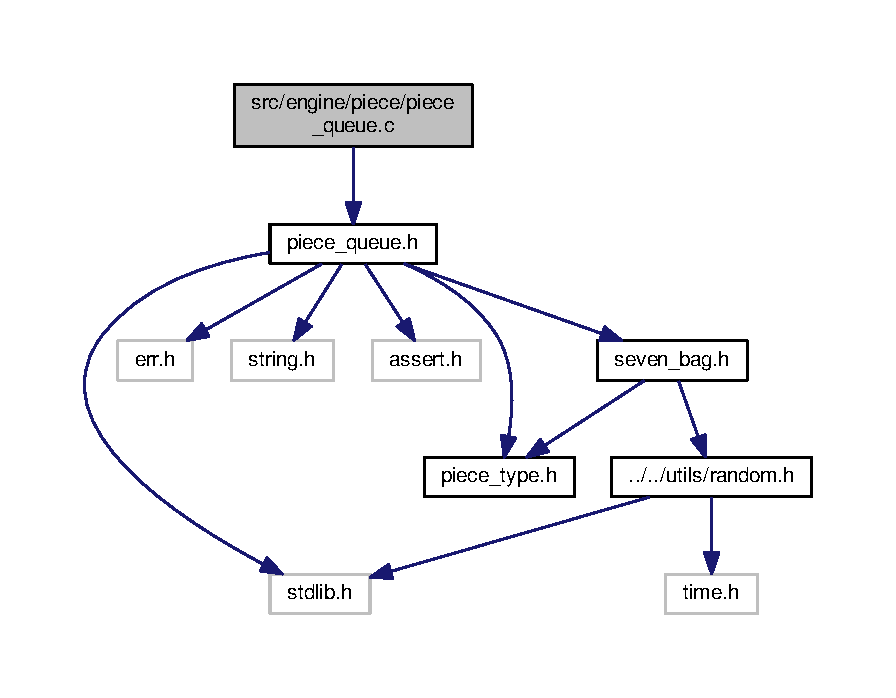
\includegraphics[width=350pt]{piece__queue_8c__incl}
\end{center}
\end{figure}
\subsection*{Functions}
\begin{DoxyCompactItemize}
\item 
\textbf{ Piece\+Queue} $\ast$ \textbf{ piece\+\_\+queue\+\_\+create} ()
\item 
void \textbf{ piece\+\_\+queue\+\_\+free} (\textbf{ Piece\+Queue} $\ast$q)
\item 
void \textbf{ piece\+\_\+queue\+\_\+fill\+\_\+data} (\textbf{ Piece\+Type} $\ast$data, size\+\_\+t length)
\item 
void \textbf{ piece\+\_\+queue\+\_\+extend} (\textbf{ Piece\+Queue} $\ast$q)
\item 
\textbf{ Piece\+Type} \textbf{ piece\+\_\+queue\+\_\+get} (\textbf{ Piece\+Queue} $\ast$q, size\+\_\+t index)
\end{DoxyCompactItemize}


\subsection{Detailed Description}
\doxyref{Piece}{p.}{structPiece} queue. 

\begin{DoxyAuthor}{Author}
S4\+Master\+Race 
\end{DoxyAuthor}
\begin{DoxyVersion}{Version}
2.\+0 
\end{DoxyVersion}


\subsection{Function Documentation}
\mbox{\label{piece__queue_8c_a0ec6b38d3854de4ace8f6b2e01680f20}} 
\index{piece\+\_\+queue.\+c@{piece\+\_\+queue.\+c}!piece\+\_\+queue\+\_\+create@{piece\+\_\+queue\+\_\+create}}
\index{piece\+\_\+queue\+\_\+create@{piece\+\_\+queue\+\_\+create}!piece\+\_\+queue.\+c@{piece\+\_\+queue.\+c}}
\subsubsection{piece\+\_\+queue\+\_\+create()}
{\footnotesize\ttfamily \textbf{ Piece\+Queue}$\ast$ piece\+\_\+queue\+\_\+create (\begin{DoxyParamCaption}{ }\end{DoxyParamCaption})}

\mbox{\label{piece__queue_8c_ad190d79bc43e6879e028443afb1e2c3b}} 
\index{piece\+\_\+queue.\+c@{piece\+\_\+queue.\+c}!piece\+\_\+queue\+\_\+extend@{piece\+\_\+queue\+\_\+extend}}
\index{piece\+\_\+queue\+\_\+extend@{piece\+\_\+queue\+\_\+extend}!piece\+\_\+queue.\+c@{piece\+\_\+queue.\+c}}
\subsubsection{piece\+\_\+queue\+\_\+extend()}
{\footnotesize\ttfamily void piece\+\_\+queue\+\_\+extend (\begin{DoxyParamCaption}\item[{\textbf{ Piece\+Queue} $\ast$}]{q }\end{DoxyParamCaption})}

\mbox{\label{piece__queue_8c_a36d95c6807746731bf8ded376b7b95c3}} 
\index{piece\+\_\+queue.\+c@{piece\+\_\+queue.\+c}!piece\+\_\+queue\+\_\+fill\+\_\+data@{piece\+\_\+queue\+\_\+fill\+\_\+data}}
\index{piece\+\_\+queue\+\_\+fill\+\_\+data@{piece\+\_\+queue\+\_\+fill\+\_\+data}!piece\+\_\+queue.\+c@{piece\+\_\+queue.\+c}}
\subsubsection{piece\+\_\+queue\+\_\+fill\+\_\+data()}
{\footnotesize\ttfamily void piece\+\_\+queue\+\_\+fill\+\_\+data (\begin{DoxyParamCaption}\item[{\textbf{ Piece\+Type} $\ast$}]{data,  }\item[{size\+\_\+t}]{length }\end{DoxyParamCaption})}

\mbox{\label{piece__queue_8c_a95d35265b3f087d3b362dd695542f596}} 
\index{piece\+\_\+queue.\+c@{piece\+\_\+queue.\+c}!piece\+\_\+queue\+\_\+free@{piece\+\_\+queue\+\_\+free}}
\index{piece\+\_\+queue\+\_\+free@{piece\+\_\+queue\+\_\+free}!piece\+\_\+queue.\+c@{piece\+\_\+queue.\+c}}
\subsubsection{piece\+\_\+queue\+\_\+free()}
{\footnotesize\ttfamily void piece\+\_\+queue\+\_\+free (\begin{DoxyParamCaption}\item[{\textbf{ Piece\+Queue} $\ast$}]{q }\end{DoxyParamCaption})}

\mbox{\label{piece__queue_8c_a53855252b8c81561fb182e3f723b5b2e}} 
\index{piece\+\_\+queue.\+c@{piece\+\_\+queue.\+c}!piece\+\_\+queue\+\_\+get@{piece\+\_\+queue\+\_\+get}}
\index{piece\+\_\+queue\+\_\+get@{piece\+\_\+queue\+\_\+get}!piece\+\_\+queue.\+c@{piece\+\_\+queue.\+c}}
\subsubsection{piece\+\_\+queue\+\_\+get()}
{\footnotesize\ttfamily \textbf{ Piece\+Type} piece\+\_\+queue\+\_\+get (\begin{DoxyParamCaption}\item[{\textbf{ Piece\+Queue} $\ast$}]{q,  }\item[{size\+\_\+t}]{index }\end{DoxyParamCaption})}


\section{src/engine/piece/piece\+\_\+queue.h File Reference}
\label{piece__queue_8h}\index{src/engine/piece/piece\+\_\+queue.\+h@{src/engine/piece/piece\+\_\+queue.\+h}}


\doxyref{Piece}{p.}{structPiece} queue.  


{\ttfamily \#include $<$stdlib.\+h$>$}\newline
{\ttfamily \#include $<$err.\+h$>$}\newline
{\ttfamily \#include $<$string.\+h$>$}\newline
{\ttfamily \#include $<$assert.\+h$>$}\newline
{\ttfamily \#include \char`\"{}piece\+\_\+type.\+h\char`\"{}}\newline
{\ttfamily \#include \char`\"{}seven\+\_\+bag.\+h\char`\"{}}\newline
Include dependency graph for piece\+\_\+queue.\+h\+:
\nopagebreak
\begin{figure}[H]
\begin{center}
\leavevmode
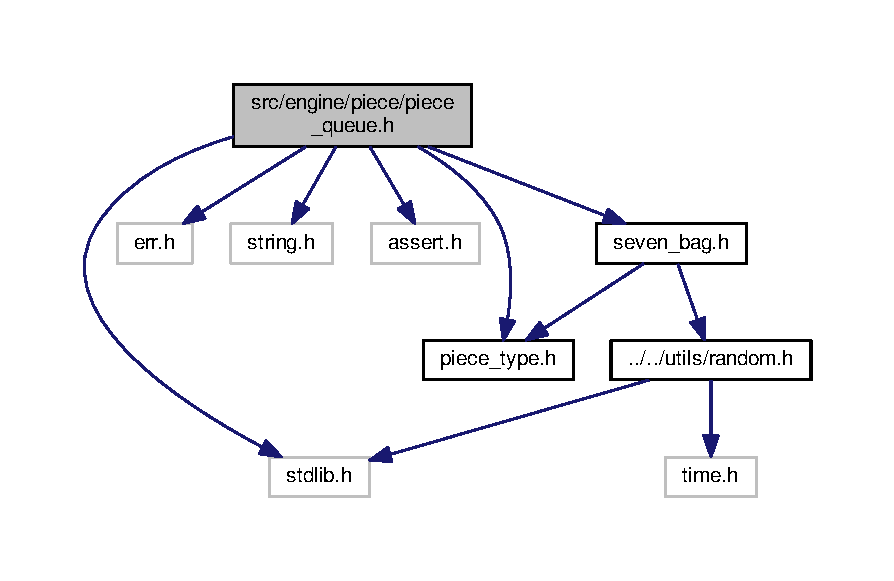
\includegraphics[width=350pt]{piece__queue_8h__incl}
\end{center}
\end{figure}
This graph shows which files directly or indirectly include this file\+:
\nopagebreak
\begin{figure}[H]
\begin{center}
\leavevmode
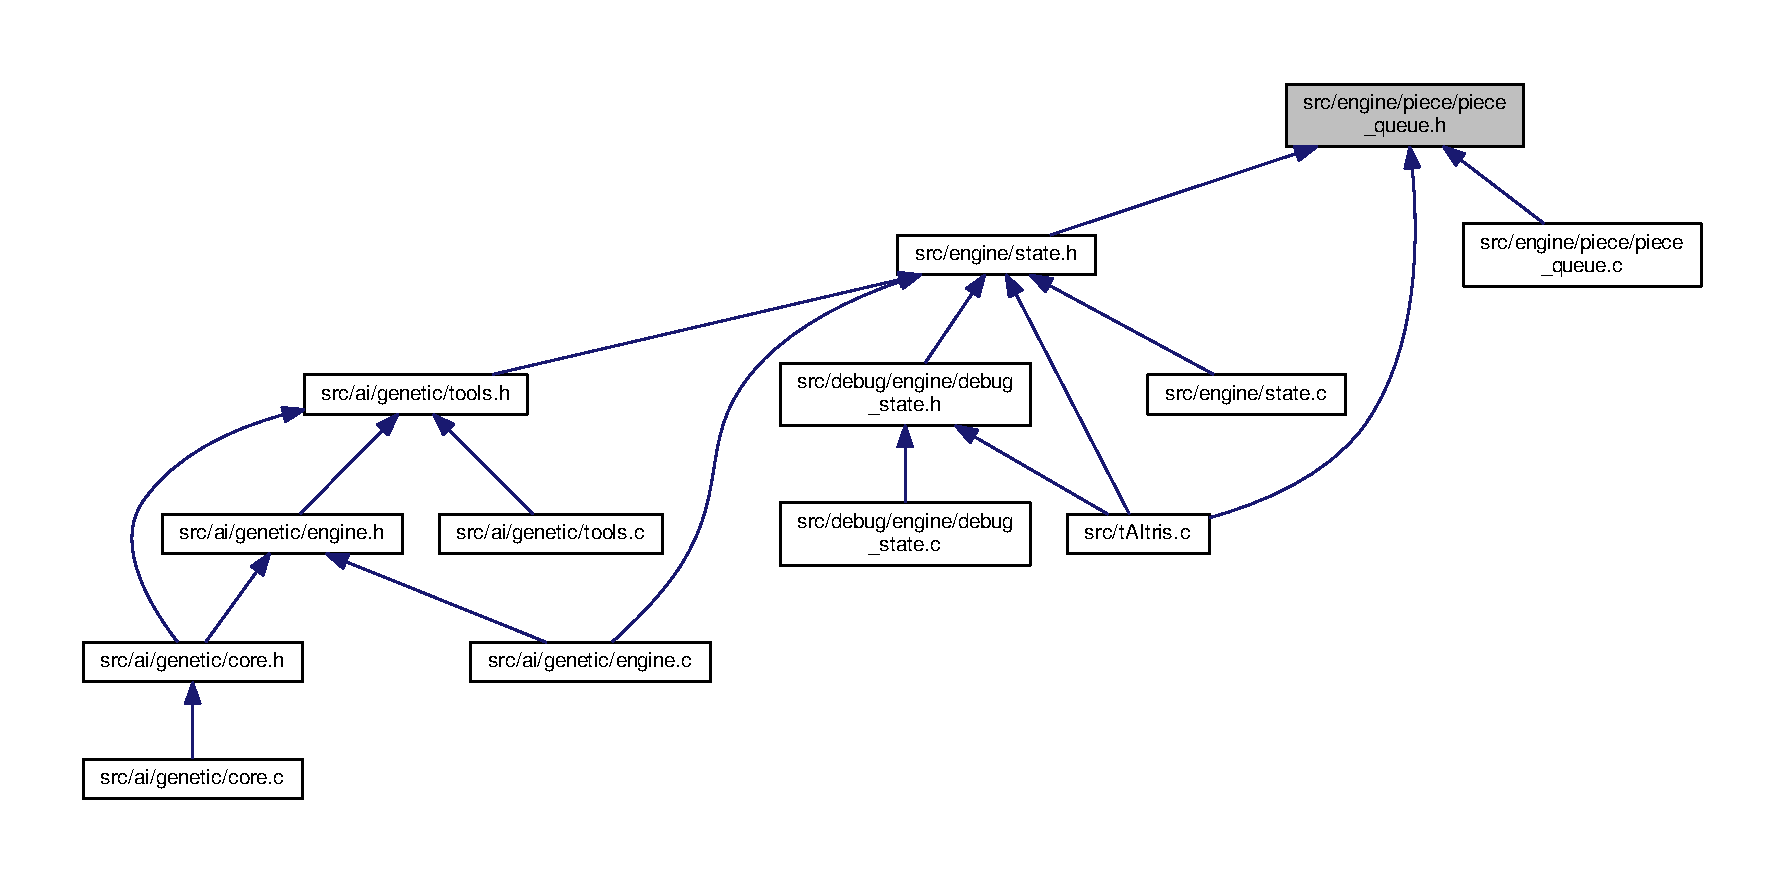
\includegraphics[width=350pt]{piece__queue_8h__dep__incl}
\end{center}
\end{figure}
\subsection*{Data Structures}
\begin{DoxyCompactItemize}
\item 
struct \textbf{ Piece\+Queue}
\end{DoxyCompactItemize}
\subsection*{Macros}
\begin{DoxyCompactItemize}
\item 
\#define \textbf{ P\+I\+E\+C\+E\+\_\+\+Q\+U\+E\+U\+E\+\_\+\+L\+E\+N\+G\+TH}~100
\end{DoxyCompactItemize}
\subsection*{Functions}
\begin{DoxyCompactItemize}
\item 
\textbf{ Piece\+Queue} $\ast$ \textbf{ piece\+\_\+queue\+\_\+create} ()
\item 
void \textbf{ piece\+\_\+queue\+\_\+free} (\textbf{ Piece\+Queue} $\ast$q)
\item 
void \textbf{ piece\+\_\+queue\+\_\+fill\+\_\+data} (\textbf{ Piece\+Type} $\ast$data, size\+\_\+t length)
\item 
void \textbf{ piece\+\_\+queue\+\_\+extend} (\textbf{ Piece\+Queue} $\ast$q)
\item 
\textbf{ Piece\+Type} \textbf{ piece\+\_\+queue\+\_\+get} (\textbf{ Piece\+Queue} $\ast$q, size\+\_\+t index)
\end{DoxyCompactItemize}


\subsection{Detailed Description}
\doxyref{Piece}{p.}{structPiece} queue. 

\begin{DoxyAuthor}{Author}
S4\+Master\+Race 
\end{DoxyAuthor}
\begin{DoxyVersion}{Version}
2.\+0 
\end{DoxyVersion}


\subsection{Macro Definition Documentation}
\mbox{\label{piece__queue_8h_ab1ad9003c6e3b971b9a3fc120c66df30}} 
\index{piece\+\_\+queue.\+h@{piece\+\_\+queue.\+h}!P\+I\+E\+C\+E\+\_\+\+Q\+U\+E\+U\+E\+\_\+\+L\+E\+N\+G\+TH@{P\+I\+E\+C\+E\+\_\+\+Q\+U\+E\+U\+E\+\_\+\+L\+E\+N\+G\+TH}}
\index{P\+I\+E\+C\+E\+\_\+\+Q\+U\+E\+U\+E\+\_\+\+L\+E\+N\+G\+TH@{P\+I\+E\+C\+E\+\_\+\+Q\+U\+E\+U\+E\+\_\+\+L\+E\+N\+G\+TH}!piece\+\_\+queue.\+h@{piece\+\_\+queue.\+h}}
\subsubsection{P\+I\+E\+C\+E\+\_\+\+Q\+U\+E\+U\+E\+\_\+\+L\+E\+N\+G\+TH}
{\footnotesize\ttfamily \#define P\+I\+E\+C\+E\+\_\+\+Q\+U\+E\+U\+E\+\_\+\+L\+E\+N\+G\+TH~100}



\subsection{Function Documentation}
\mbox{\label{piece__queue_8h_a0ec6b38d3854de4ace8f6b2e01680f20}} 
\index{piece\+\_\+queue.\+h@{piece\+\_\+queue.\+h}!piece\+\_\+queue\+\_\+create@{piece\+\_\+queue\+\_\+create}}
\index{piece\+\_\+queue\+\_\+create@{piece\+\_\+queue\+\_\+create}!piece\+\_\+queue.\+h@{piece\+\_\+queue.\+h}}
\subsubsection{piece\+\_\+queue\+\_\+create()}
{\footnotesize\ttfamily \textbf{ Piece\+Queue}$\ast$ piece\+\_\+queue\+\_\+create (\begin{DoxyParamCaption}{ }\end{DoxyParamCaption})}

\mbox{\label{piece__queue_8h_ad190d79bc43e6879e028443afb1e2c3b}} 
\index{piece\+\_\+queue.\+h@{piece\+\_\+queue.\+h}!piece\+\_\+queue\+\_\+extend@{piece\+\_\+queue\+\_\+extend}}
\index{piece\+\_\+queue\+\_\+extend@{piece\+\_\+queue\+\_\+extend}!piece\+\_\+queue.\+h@{piece\+\_\+queue.\+h}}
\subsubsection{piece\+\_\+queue\+\_\+extend()}
{\footnotesize\ttfamily void piece\+\_\+queue\+\_\+extend (\begin{DoxyParamCaption}\item[{\textbf{ Piece\+Queue} $\ast$}]{q }\end{DoxyParamCaption})}

\mbox{\label{piece__queue_8h_a36d95c6807746731bf8ded376b7b95c3}} 
\index{piece\+\_\+queue.\+h@{piece\+\_\+queue.\+h}!piece\+\_\+queue\+\_\+fill\+\_\+data@{piece\+\_\+queue\+\_\+fill\+\_\+data}}
\index{piece\+\_\+queue\+\_\+fill\+\_\+data@{piece\+\_\+queue\+\_\+fill\+\_\+data}!piece\+\_\+queue.\+h@{piece\+\_\+queue.\+h}}
\subsubsection{piece\+\_\+queue\+\_\+fill\+\_\+data()}
{\footnotesize\ttfamily void piece\+\_\+queue\+\_\+fill\+\_\+data (\begin{DoxyParamCaption}\item[{\textbf{ Piece\+Type} $\ast$}]{data,  }\item[{size\+\_\+t}]{length }\end{DoxyParamCaption})}

\mbox{\label{piece__queue_8h_a95d35265b3f087d3b362dd695542f596}} 
\index{piece\+\_\+queue.\+h@{piece\+\_\+queue.\+h}!piece\+\_\+queue\+\_\+free@{piece\+\_\+queue\+\_\+free}}
\index{piece\+\_\+queue\+\_\+free@{piece\+\_\+queue\+\_\+free}!piece\+\_\+queue.\+h@{piece\+\_\+queue.\+h}}
\subsubsection{piece\+\_\+queue\+\_\+free()}
{\footnotesize\ttfamily void piece\+\_\+queue\+\_\+free (\begin{DoxyParamCaption}\item[{\textbf{ Piece\+Queue} $\ast$}]{q }\end{DoxyParamCaption})}

\mbox{\label{piece__queue_8h_a53855252b8c81561fb182e3f723b5b2e}} 
\index{piece\+\_\+queue.\+h@{piece\+\_\+queue.\+h}!piece\+\_\+queue\+\_\+get@{piece\+\_\+queue\+\_\+get}}
\index{piece\+\_\+queue\+\_\+get@{piece\+\_\+queue\+\_\+get}!piece\+\_\+queue.\+h@{piece\+\_\+queue.\+h}}
\subsubsection{piece\+\_\+queue\+\_\+get()}
{\footnotesize\ttfamily \textbf{ Piece\+Type} piece\+\_\+queue\+\_\+get (\begin{DoxyParamCaption}\item[{\textbf{ Piece\+Queue} $\ast$}]{q,  }\item[{size\+\_\+t}]{index }\end{DoxyParamCaption})}


\section{src/engine/piece/piece\+\_\+shape.h File Reference}
\label{piece__shape_8h}\index{src/engine/piece/piece\+\_\+shape.\+h@{src/engine/piece/piece\+\_\+shape.\+h}}


\doxyref{Piece}{p.}{structPiece} shape.  


{\ttfamily \#include $<$stdlib.\+h$>$}\newline
{\ttfamily \#include $<$err.\+h$>$}\newline
{\ttfamily \#include \char`\"{}../cell.\+h\char`\"{}}\newline
{\ttfamily \#include \char`\"{}../angle.\+h\char`\"{}}\newline
{\ttfamily \#include \char`\"{}piece\+\_\+type.\+h\char`\"{}}\newline
Include dependency graph for piece\+\_\+shape.\+h\+:
\nopagebreak
\begin{figure}[H]
\begin{center}
\leavevmode
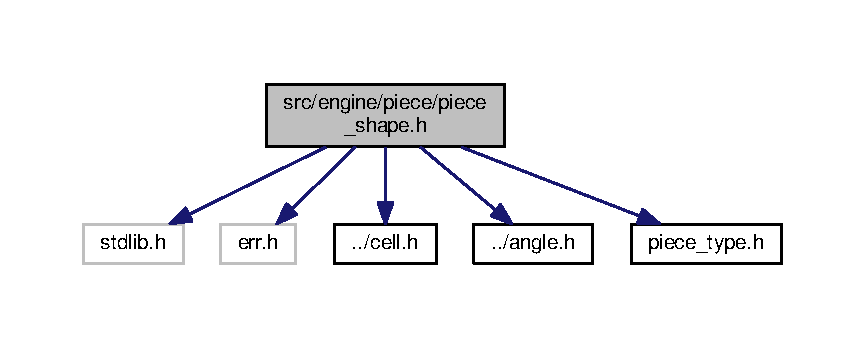
\includegraphics[width=350pt]{piece__shape_8h__incl}
\end{center}
\end{figure}
This graph shows which files directly or indirectly include this file\+:
\nopagebreak
\begin{figure}[H]
\begin{center}
\leavevmode
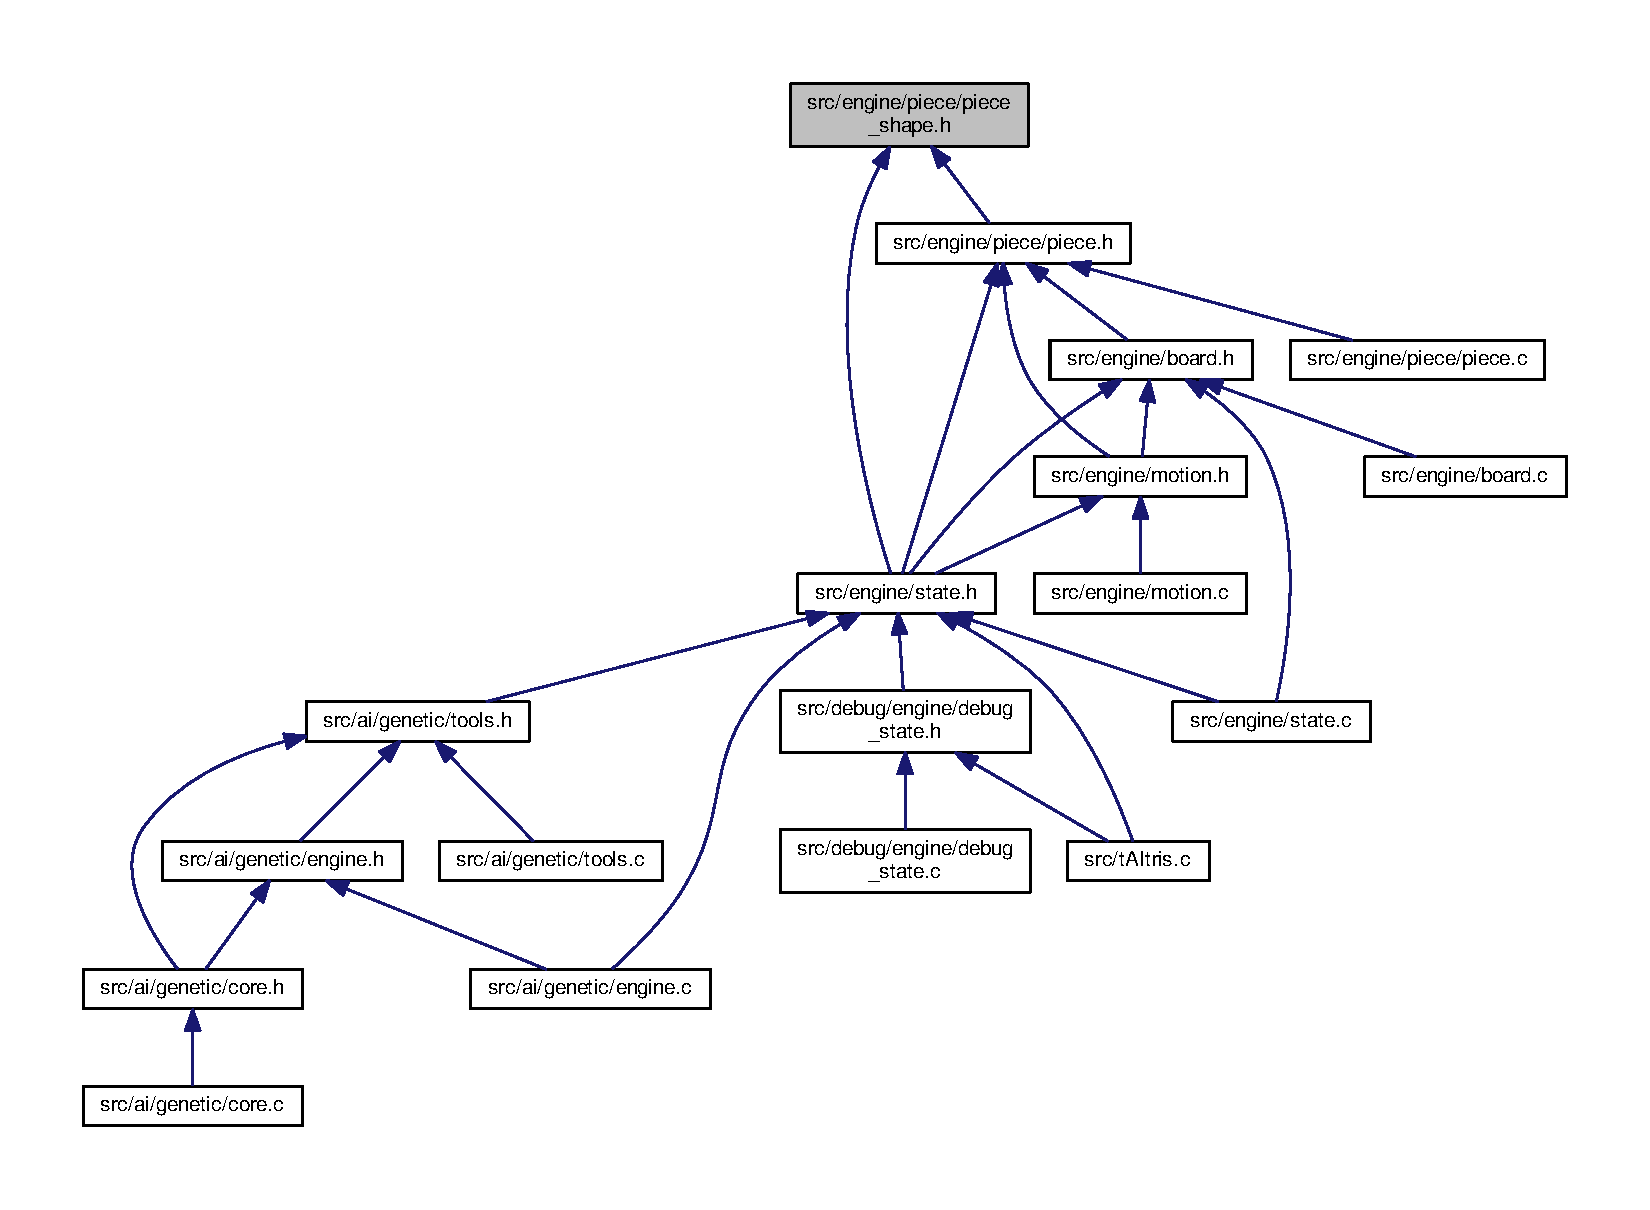
\includegraphics[width=350pt]{piece__shape_8h__dep__incl}
\end{center}
\end{figure}
\subsection*{Data Structures}
\begin{DoxyCompactItemize}
\item 
struct \textbf{ Piece\+Shape}
\end{DoxyCompactItemize}
\subsection*{Macros}
\begin{DoxyCompactItemize}
\item 
\#define \textbf{ P\+I\+E\+C\+E\+\_\+\+S\+H\+A\+P\+E\+\_\+\+W\+I\+D\+TH}~4
\item 
\#define \textbf{ P\+I\+E\+C\+E\+\_\+\+S\+H\+A\+P\+E\+\_\+\+H\+E\+I\+G\+HT}~4
\end{DoxyCompactItemize}


\subsection{Detailed Description}
\doxyref{Piece}{p.}{structPiece} shape. 

\begin{DoxyAuthor}{Author}
S4\+Master\+Race 
\end{DoxyAuthor}
\begin{DoxyVersion}{Version}
2.\+0 
\end{DoxyVersion}


\subsection{Macro Definition Documentation}
\mbox{\label{piece__shape_8h_a296ac2a02c276d934200fbd05315bc31}} 
\index{piece\+\_\+shape.\+h@{piece\+\_\+shape.\+h}!P\+I\+E\+C\+E\+\_\+\+S\+H\+A\+P\+E\+\_\+\+H\+E\+I\+G\+HT@{P\+I\+E\+C\+E\+\_\+\+S\+H\+A\+P\+E\+\_\+\+H\+E\+I\+G\+HT}}
\index{P\+I\+E\+C\+E\+\_\+\+S\+H\+A\+P\+E\+\_\+\+H\+E\+I\+G\+HT@{P\+I\+E\+C\+E\+\_\+\+S\+H\+A\+P\+E\+\_\+\+H\+E\+I\+G\+HT}!piece\+\_\+shape.\+h@{piece\+\_\+shape.\+h}}
\subsubsection{P\+I\+E\+C\+E\+\_\+\+S\+H\+A\+P\+E\+\_\+\+H\+E\+I\+G\+HT}
{\footnotesize\ttfamily \#define P\+I\+E\+C\+E\+\_\+\+S\+H\+A\+P\+E\+\_\+\+H\+E\+I\+G\+HT~4}

\mbox{\label{piece__shape_8h_a3452ee75c742f0efcd15b3138182dd28}} 
\index{piece\+\_\+shape.\+h@{piece\+\_\+shape.\+h}!P\+I\+E\+C\+E\+\_\+\+S\+H\+A\+P\+E\+\_\+\+W\+I\+D\+TH@{P\+I\+E\+C\+E\+\_\+\+S\+H\+A\+P\+E\+\_\+\+W\+I\+D\+TH}}
\index{P\+I\+E\+C\+E\+\_\+\+S\+H\+A\+P\+E\+\_\+\+W\+I\+D\+TH@{P\+I\+E\+C\+E\+\_\+\+S\+H\+A\+P\+E\+\_\+\+W\+I\+D\+TH}!piece\+\_\+shape.\+h@{piece\+\_\+shape.\+h}}
\subsubsection{P\+I\+E\+C\+E\+\_\+\+S\+H\+A\+P\+E\+\_\+\+W\+I\+D\+TH}
{\footnotesize\ttfamily \#define P\+I\+E\+C\+E\+\_\+\+S\+H\+A\+P\+E\+\_\+\+W\+I\+D\+TH~4}


\section{src/engine/piece/piece\+\_\+type.h File Reference}
\label{piece__type_8h}\index{src/engine/piece/piece\+\_\+type.\+h@{src/engine/piece/piece\+\_\+type.\+h}}


\doxyref{Piece}{p.}{structPiece} type.  


This graph shows which files directly or indirectly include this file\+:
\nopagebreak
\begin{figure}[H]
\begin{center}
\leavevmode
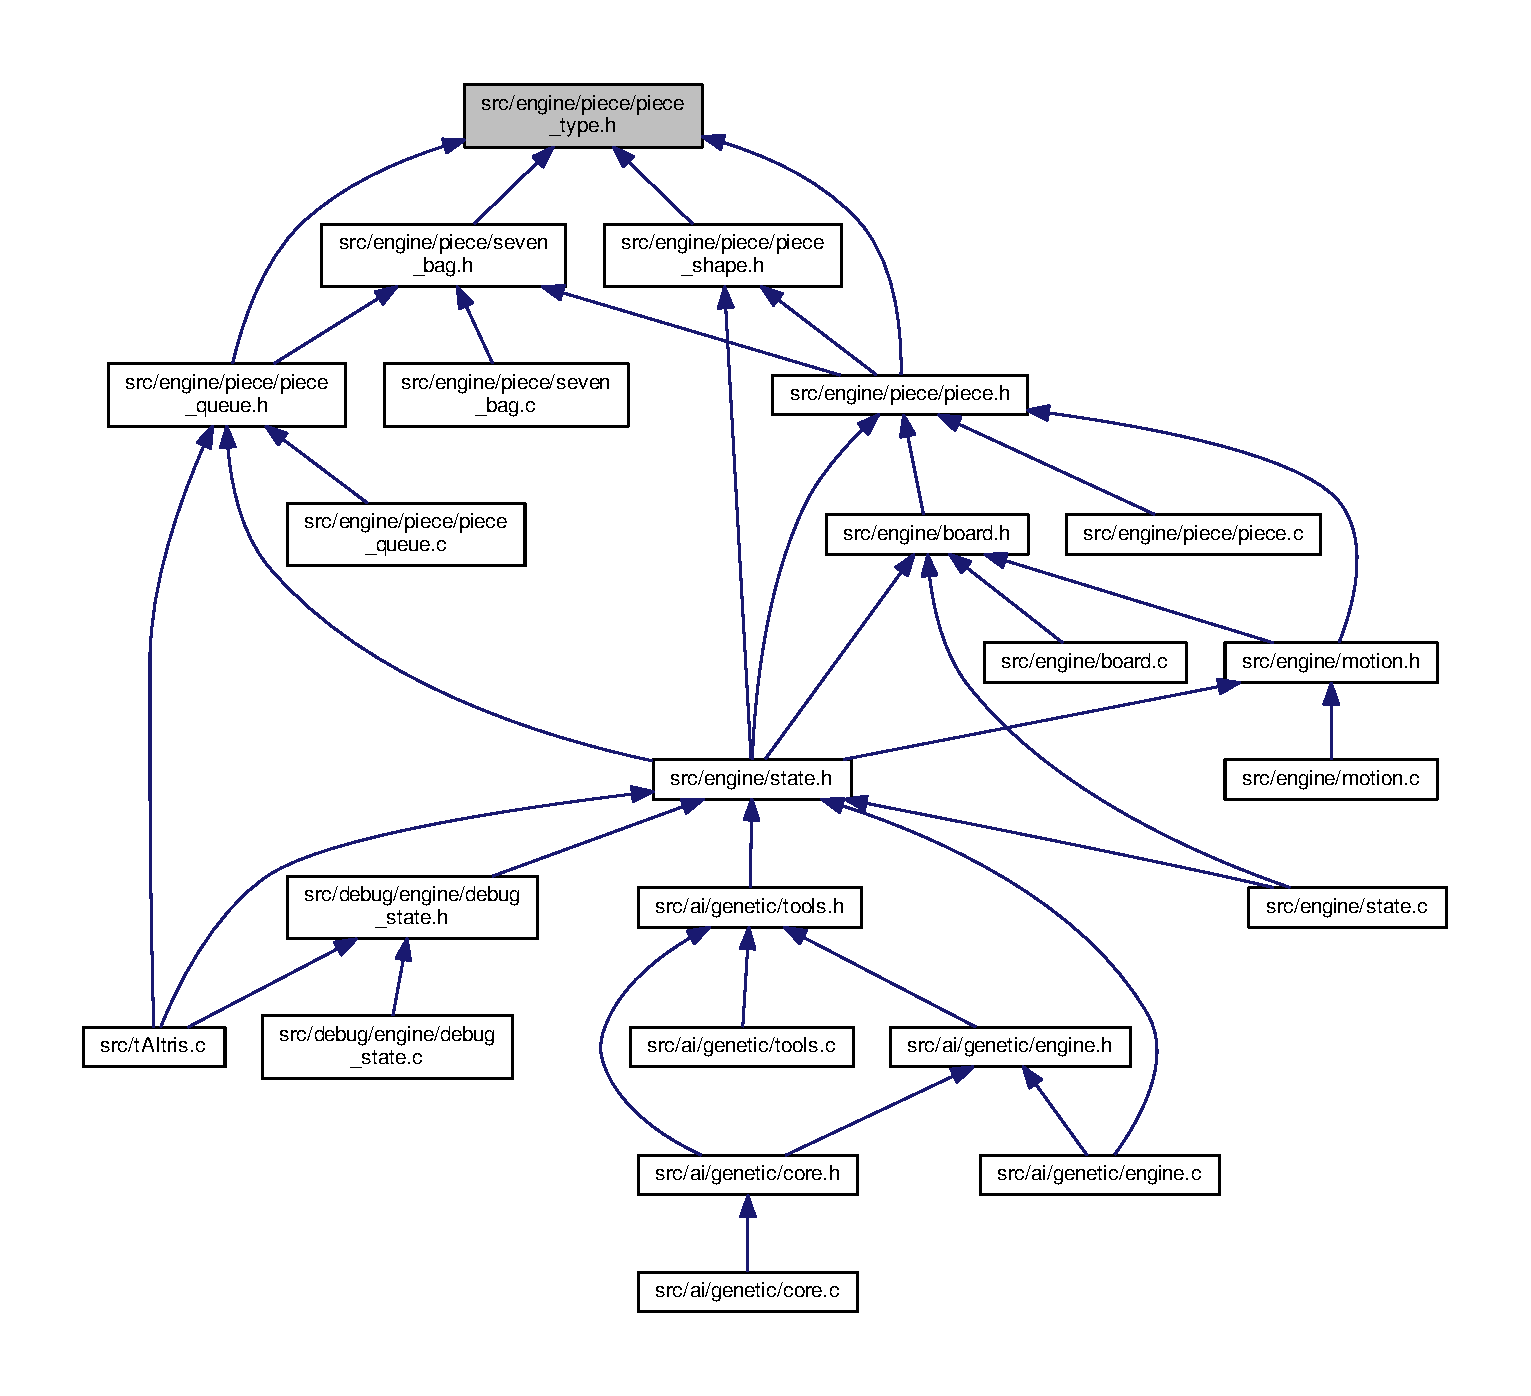
\includegraphics[width=350pt]{piece__type_8h__dep__incl}
\end{center}
\end{figure}
\subsection*{Macros}
\begin{DoxyCompactItemize}
\item 
\#define \textbf{ P\+I\+E\+C\+E\+\_\+\+T\+Y\+P\+E\+\_\+\+E\+S\+I\+ZE}~7
\end{DoxyCompactItemize}
\subsection*{Enumerations}
\begin{DoxyCompactItemize}
\item 
enum \textbf{ Piece\+Type} \{ \newline
\textbf{ P\+I\+E\+C\+E\+\_\+\+T\+Y\+P\+E\+\_\+I}, 
\textbf{ P\+I\+E\+C\+E\+\_\+\+T\+Y\+P\+E\+\_\+O}, 
\textbf{ P\+I\+E\+C\+E\+\_\+\+T\+Y\+P\+E\+\_\+T}, 
\textbf{ P\+I\+E\+C\+E\+\_\+\+T\+Y\+P\+E\+\_\+L}, 
\newline
\textbf{ P\+I\+E\+C\+E\+\_\+\+T\+Y\+P\+E\+\_\+J}, 
\textbf{ P\+I\+E\+C\+E\+\_\+\+T\+Y\+P\+E\+\_\+Z}, 
\textbf{ P\+I\+E\+C\+E\+\_\+\+T\+Y\+P\+E\+\_\+S}
 \}
\end{DoxyCompactItemize}


\subsection{Detailed Description}
\doxyref{Piece}{p.}{structPiece} type. 

\begin{DoxyAuthor}{Author}
S4\+Master\+Race 
\end{DoxyAuthor}
\begin{DoxyVersion}{Version}
2.\+0 
\end{DoxyVersion}


\subsection{Macro Definition Documentation}
\mbox{\label{piece__type_8h_a93319ded5c88fcd7fe1f9c7a5de0f46e}} 
\index{piece\+\_\+type.\+h@{piece\+\_\+type.\+h}!P\+I\+E\+C\+E\+\_\+\+T\+Y\+P\+E\+\_\+\+E\+S\+I\+ZE@{P\+I\+E\+C\+E\+\_\+\+T\+Y\+P\+E\+\_\+\+E\+S\+I\+ZE}}
\index{P\+I\+E\+C\+E\+\_\+\+T\+Y\+P\+E\+\_\+\+E\+S\+I\+ZE@{P\+I\+E\+C\+E\+\_\+\+T\+Y\+P\+E\+\_\+\+E\+S\+I\+ZE}!piece\+\_\+type.\+h@{piece\+\_\+type.\+h}}
\subsubsection{P\+I\+E\+C\+E\+\_\+\+T\+Y\+P\+E\+\_\+\+E\+S\+I\+ZE}
{\footnotesize\ttfamily \#define P\+I\+E\+C\+E\+\_\+\+T\+Y\+P\+E\+\_\+\+E\+S\+I\+ZE~7}



\subsection{Enumeration Type Documentation}
\mbox{\label{piece__type_8h_a12ed9719bbdf7bc596ff7a6f4bf3f021}} 
\index{piece\+\_\+type.\+h@{piece\+\_\+type.\+h}!Piece\+Type@{Piece\+Type}}
\index{Piece\+Type@{Piece\+Type}!piece\+\_\+type.\+h@{piece\+\_\+type.\+h}}
\subsubsection{Piece\+Type}
{\footnotesize\ttfamily enum \textbf{ Piece\+Type}}

\begin{DoxyEnumFields}{Enumerator}
\raisebox{\heightof{T}}[0pt][0pt]{\index{P\+I\+E\+C\+E\+\_\+\+T\+Y\+P\+E\+\_\+I@{P\+I\+E\+C\+E\+\_\+\+T\+Y\+P\+E\+\_\+I}!piece\+\_\+type.\+h@{piece\+\_\+type.\+h}}\index{piece\+\_\+type.\+h@{piece\+\_\+type.\+h}!P\+I\+E\+C\+E\+\_\+\+T\+Y\+P\+E\+\_\+I@{P\+I\+E\+C\+E\+\_\+\+T\+Y\+P\+E\+\_\+I}}}\mbox{\label{piece__type_8h_a12ed9719bbdf7bc596ff7a6f4bf3f021a6044ca3c5a8f3b2cb6e9a7d81e7b0394}} 
P\+I\+E\+C\+E\+\_\+\+T\+Y\+P\+E\+\_\+I&\\
\hline

\raisebox{\heightof{T}}[0pt][0pt]{\index{P\+I\+E\+C\+E\+\_\+\+T\+Y\+P\+E\+\_\+O@{P\+I\+E\+C\+E\+\_\+\+T\+Y\+P\+E\+\_\+O}!piece\+\_\+type.\+h@{piece\+\_\+type.\+h}}\index{piece\+\_\+type.\+h@{piece\+\_\+type.\+h}!P\+I\+E\+C\+E\+\_\+\+T\+Y\+P\+E\+\_\+O@{P\+I\+E\+C\+E\+\_\+\+T\+Y\+P\+E\+\_\+O}}}\mbox{\label{piece__type_8h_a12ed9719bbdf7bc596ff7a6f4bf3f021a9c18ca502ed476669887c896f3fd9df1}} 
P\+I\+E\+C\+E\+\_\+\+T\+Y\+P\+E\+\_\+O&\\
\hline

\raisebox{\heightof{T}}[0pt][0pt]{\index{P\+I\+E\+C\+E\+\_\+\+T\+Y\+P\+E\+\_\+T@{P\+I\+E\+C\+E\+\_\+\+T\+Y\+P\+E\+\_\+T}!piece\+\_\+type.\+h@{piece\+\_\+type.\+h}}\index{piece\+\_\+type.\+h@{piece\+\_\+type.\+h}!P\+I\+E\+C\+E\+\_\+\+T\+Y\+P\+E\+\_\+T@{P\+I\+E\+C\+E\+\_\+\+T\+Y\+P\+E\+\_\+T}}}\mbox{\label{piece__type_8h_a12ed9719bbdf7bc596ff7a6f4bf3f021ad71ccbc52fdbdbf73407bd868d921be2}} 
P\+I\+E\+C\+E\+\_\+\+T\+Y\+P\+E\+\_\+T&\\
\hline

\raisebox{\heightof{T}}[0pt][0pt]{\index{P\+I\+E\+C\+E\+\_\+\+T\+Y\+P\+E\+\_\+L@{P\+I\+E\+C\+E\+\_\+\+T\+Y\+P\+E\+\_\+L}!piece\+\_\+type.\+h@{piece\+\_\+type.\+h}}\index{piece\+\_\+type.\+h@{piece\+\_\+type.\+h}!P\+I\+E\+C\+E\+\_\+\+T\+Y\+P\+E\+\_\+L@{P\+I\+E\+C\+E\+\_\+\+T\+Y\+P\+E\+\_\+L}}}\mbox{\label{piece__type_8h_a12ed9719bbdf7bc596ff7a6f4bf3f021a8bbd1e7f2e0f4c5ab1e15e670ddce63b}} 
P\+I\+E\+C\+E\+\_\+\+T\+Y\+P\+E\+\_\+L&\\
\hline

\raisebox{\heightof{T}}[0pt][0pt]{\index{P\+I\+E\+C\+E\+\_\+\+T\+Y\+P\+E\+\_\+J@{P\+I\+E\+C\+E\+\_\+\+T\+Y\+P\+E\+\_\+J}!piece\+\_\+type.\+h@{piece\+\_\+type.\+h}}\index{piece\+\_\+type.\+h@{piece\+\_\+type.\+h}!P\+I\+E\+C\+E\+\_\+\+T\+Y\+P\+E\+\_\+J@{P\+I\+E\+C\+E\+\_\+\+T\+Y\+P\+E\+\_\+J}}}\mbox{\label{piece__type_8h_a12ed9719bbdf7bc596ff7a6f4bf3f021a9d6ac5d6468d6f2e6b78f039910772f0}} 
P\+I\+E\+C\+E\+\_\+\+T\+Y\+P\+E\+\_\+J&\\
\hline

\raisebox{\heightof{T}}[0pt][0pt]{\index{P\+I\+E\+C\+E\+\_\+\+T\+Y\+P\+E\+\_\+Z@{P\+I\+E\+C\+E\+\_\+\+T\+Y\+P\+E\+\_\+Z}!piece\+\_\+type.\+h@{piece\+\_\+type.\+h}}\index{piece\+\_\+type.\+h@{piece\+\_\+type.\+h}!P\+I\+E\+C\+E\+\_\+\+T\+Y\+P\+E\+\_\+Z@{P\+I\+E\+C\+E\+\_\+\+T\+Y\+P\+E\+\_\+Z}}}\mbox{\label{piece__type_8h_a12ed9719bbdf7bc596ff7a6f4bf3f021a254222355d4ba35ecc53d9e5ef4dc39d}} 
P\+I\+E\+C\+E\+\_\+\+T\+Y\+P\+E\+\_\+Z&\\
\hline

\raisebox{\heightof{T}}[0pt][0pt]{\index{P\+I\+E\+C\+E\+\_\+\+T\+Y\+P\+E\+\_\+S@{P\+I\+E\+C\+E\+\_\+\+T\+Y\+P\+E\+\_\+S}!piece\+\_\+type.\+h@{piece\+\_\+type.\+h}}\index{piece\+\_\+type.\+h@{piece\+\_\+type.\+h}!P\+I\+E\+C\+E\+\_\+\+T\+Y\+P\+E\+\_\+S@{P\+I\+E\+C\+E\+\_\+\+T\+Y\+P\+E\+\_\+S}}}\mbox{\label{piece__type_8h_a12ed9719bbdf7bc596ff7a6f4bf3f021a93cb32c97b46e806fccd40e32e0a74a8}} 
P\+I\+E\+C\+E\+\_\+\+T\+Y\+P\+E\+\_\+S&\\
\hline

\end{DoxyEnumFields}

\section{src/engine/piece/seven\+\_\+bag.c File Reference}
\label{seven__bag_8c}\index{src/engine/piece/seven\+\_\+bag.\+c@{src/engine/piece/seven\+\_\+bag.\+c}}


7-\/\+Bag generator  


{\ttfamily \#include \char`\"{}seven\+\_\+bag.\+h\char`\"{}}\newline
Include dependency graph for seven\+\_\+bag.\+c\+:
\nopagebreak
\begin{figure}[H]
\begin{center}
\leavevmode
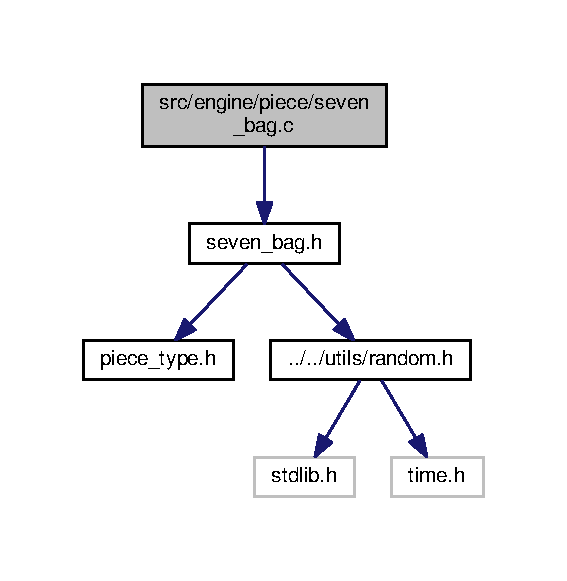
\includegraphics[width=272pt]{seven__bag_8c__incl}
\end{center}
\end{figure}
\subsection*{Functions}
\begin{DoxyCompactItemize}
\item 
void \textbf{ seven\+\_\+bag\+\_\+init} (\textbf{ Piece\+Type} $\ast$bag)
\item 
void \textbf{ seven\+\_\+bag\+\_\+swap} (\textbf{ Piece\+Type} $\ast$a, \textbf{ Piece\+Type} $\ast$b)
\item 
void \textbf{ seven\+\_\+bag\+\_\+shuffle} (\textbf{ Piece\+Type} $\ast$bag)
\item 
\textbf{ Piece\+Type} \textbf{ seven\+\_\+bag\+\_\+draw} ()
\end{DoxyCompactItemize}


\subsection{Detailed Description}
7-\/\+Bag generator 

\begin{DoxyAuthor}{Author}
S4\+Master\+Race 
\end{DoxyAuthor}
\begin{DoxyVersion}{Version}
2.\+0 
\end{DoxyVersion}


\subsection{Function Documentation}
\mbox{\label{seven__bag_8c_a0da96f6a10a01d042e8b9487adb170d2}} 
\index{seven\+\_\+bag.\+c@{seven\+\_\+bag.\+c}!seven\+\_\+bag\+\_\+draw@{seven\+\_\+bag\+\_\+draw}}
\index{seven\+\_\+bag\+\_\+draw@{seven\+\_\+bag\+\_\+draw}!seven\+\_\+bag.\+c@{seven\+\_\+bag.\+c}}
\subsubsection{seven\+\_\+bag\+\_\+draw()}
{\footnotesize\ttfamily \textbf{ Piece\+Type} seven\+\_\+bag\+\_\+draw (\begin{DoxyParamCaption}{ }\end{DoxyParamCaption})}

\mbox{\label{seven__bag_8c_aaae86f9bd2c910ea459ee626ab35ad28}} 
\index{seven\+\_\+bag.\+c@{seven\+\_\+bag.\+c}!seven\+\_\+bag\+\_\+init@{seven\+\_\+bag\+\_\+init}}
\index{seven\+\_\+bag\+\_\+init@{seven\+\_\+bag\+\_\+init}!seven\+\_\+bag.\+c@{seven\+\_\+bag.\+c}}
\subsubsection{seven\+\_\+bag\+\_\+init()}
{\footnotesize\ttfamily void seven\+\_\+bag\+\_\+init (\begin{DoxyParamCaption}\item[{\textbf{ Piece\+Type} $\ast$}]{bag }\end{DoxyParamCaption})}

\mbox{\label{seven__bag_8c_a0db30dac70a7e9953f3709d2d12eeb0f}} 
\index{seven\+\_\+bag.\+c@{seven\+\_\+bag.\+c}!seven\+\_\+bag\+\_\+shuffle@{seven\+\_\+bag\+\_\+shuffle}}
\index{seven\+\_\+bag\+\_\+shuffle@{seven\+\_\+bag\+\_\+shuffle}!seven\+\_\+bag.\+c@{seven\+\_\+bag.\+c}}
\subsubsection{seven\+\_\+bag\+\_\+shuffle()}
{\footnotesize\ttfamily void seven\+\_\+bag\+\_\+shuffle (\begin{DoxyParamCaption}\item[{\textbf{ Piece\+Type} $\ast$}]{bag }\end{DoxyParamCaption})}

\mbox{\label{seven__bag_8c_a2c3087bc0bfcc740eb24edb2e36f2763}} 
\index{seven\+\_\+bag.\+c@{seven\+\_\+bag.\+c}!seven\+\_\+bag\+\_\+swap@{seven\+\_\+bag\+\_\+swap}}
\index{seven\+\_\+bag\+\_\+swap@{seven\+\_\+bag\+\_\+swap}!seven\+\_\+bag.\+c@{seven\+\_\+bag.\+c}}
\subsubsection{seven\+\_\+bag\+\_\+swap()}
{\footnotesize\ttfamily void seven\+\_\+bag\+\_\+swap (\begin{DoxyParamCaption}\item[{\textbf{ Piece\+Type} $\ast$}]{a,  }\item[{\textbf{ Piece\+Type} $\ast$}]{b }\end{DoxyParamCaption})}


\section{src/engine/piece/seven\+\_\+bag.h File Reference}
\label{seven__bag_8h}\index{src/engine/piece/seven\+\_\+bag.\+h@{src/engine/piece/seven\+\_\+bag.\+h}}


7-\/\+Bag generator  


{\ttfamily \#include \char`\"{}piece\+\_\+type.\+h\char`\"{}}\newline
{\ttfamily \#include \char`\"{}../../utils/random.\+h\char`\"{}}\newline
Include dependency graph for seven\+\_\+bag.\+h\+:
\nopagebreak
\begin{figure}[H]
\begin{center}
\leavevmode
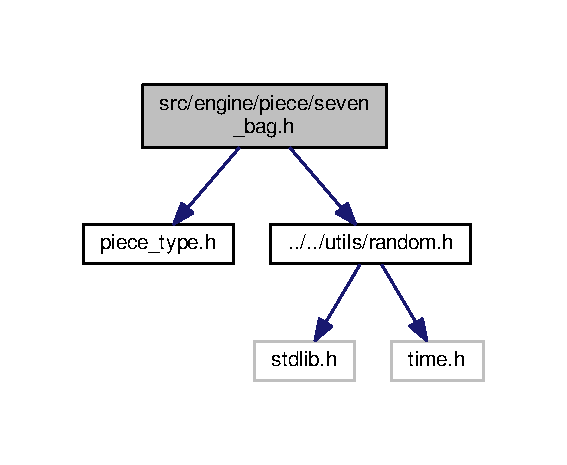
\includegraphics[width=272pt]{seven__bag_8h__incl}
\end{center}
\end{figure}
This graph shows which files directly or indirectly include this file\+:
\nopagebreak
\begin{figure}[H]
\begin{center}
\leavevmode
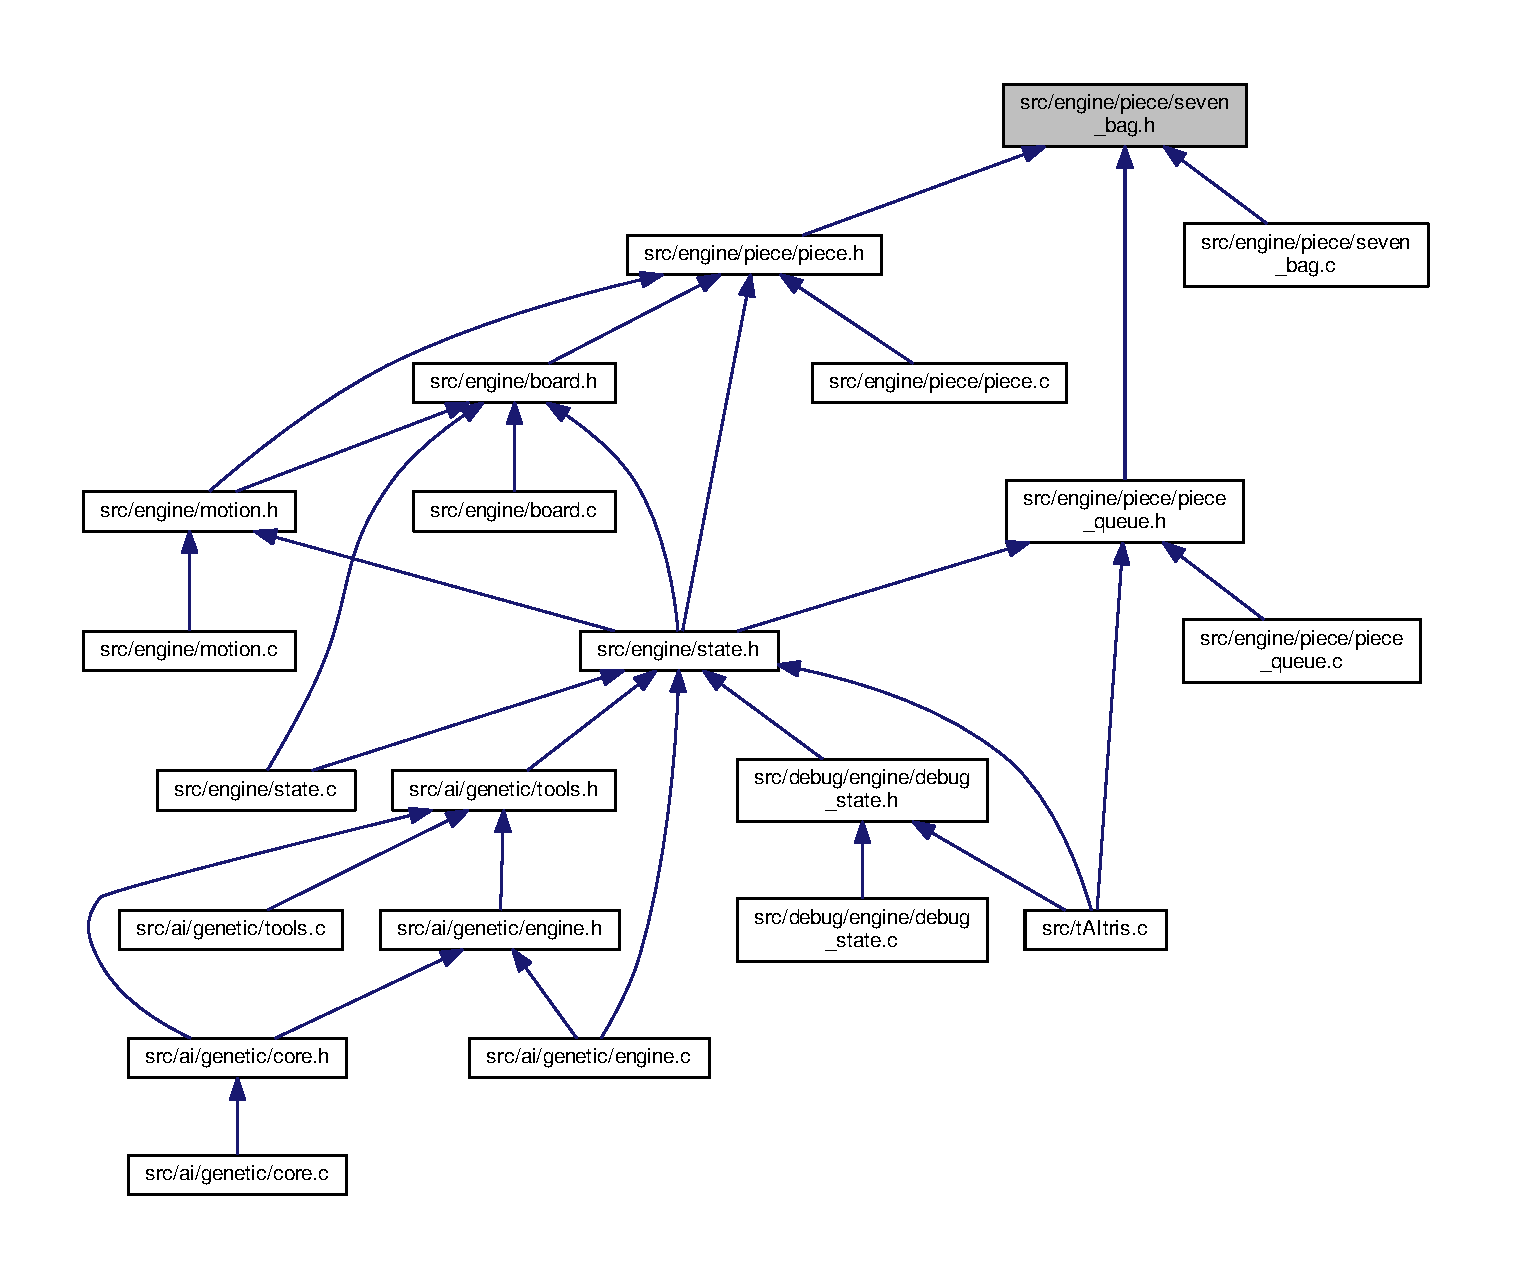
\includegraphics[width=350pt]{seven__bag_8h__dep__incl}
\end{center}
\end{figure}
\subsection*{Functions}
\begin{DoxyCompactItemize}
\item 
void \textbf{ seven\+\_\+bag\+\_\+init} (\textbf{ Piece\+Type} $\ast$bag)
\item 
void \textbf{ seven\+\_\+bag\+\_\+swap} (\textbf{ Piece\+Type} $\ast$a, \textbf{ Piece\+Type} $\ast$b)
\item 
void \textbf{ seven\+\_\+bag\+\_\+shuffle} (\textbf{ Piece\+Type} $\ast$bag)
\item 
\textbf{ Piece\+Type} \textbf{ seven\+\_\+bag\+\_\+draw} ()
\end{DoxyCompactItemize}


\subsection{Detailed Description}
7-\/\+Bag generator 

\begin{DoxyAuthor}{Author}
S4\+Master\+Race 
\end{DoxyAuthor}
\begin{DoxyVersion}{Version}
2.\+0 
\end{DoxyVersion}


\subsection{Function Documentation}
\mbox{\label{seven__bag_8h_a0da96f6a10a01d042e8b9487adb170d2}} 
\index{seven\+\_\+bag.\+h@{seven\+\_\+bag.\+h}!seven\+\_\+bag\+\_\+draw@{seven\+\_\+bag\+\_\+draw}}
\index{seven\+\_\+bag\+\_\+draw@{seven\+\_\+bag\+\_\+draw}!seven\+\_\+bag.\+h@{seven\+\_\+bag.\+h}}
\subsubsection{seven\+\_\+bag\+\_\+draw()}
{\footnotesize\ttfamily \textbf{ Piece\+Type} seven\+\_\+bag\+\_\+draw (\begin{DoxyParamCaption}{ }\end{DoxyParamCaption})}

\mbox{\label{seven__bag_8h_aaae86f9bd2c910ea459ee626ab35ad28}} 
\index{seven\+\_\+bag.\+h@{seven\+\_\+bag.\+h}!seven\+\_\+bag\+\_\+init@{seven\+\_\+bag\+\_\+init}}
\index{seven\+\_\+bag\+\_\+init@{seven\+\_\+bag\+\_\+init}!seven\+\_\+bag.\+h@{seven\+\_\+bag.\+h}}
\subsubsection{seven\+\_\+bag\+\_\+init()}
{\footnotesize\ttfamily void seven\+\_\+bag\+\_\+init (\begin{DoxyParamCaption}\item[{\textbf{ Piece\+Type} $\ast$}]{bag }\end{DoxyParamCaption})}

\mbox{\label{seven__bag_8h_a0db30dac70a7e9953f3709d2d12eeb0f}} 
\index{seven\+\_\+bag.\+h@{seven\+\_\+bag.\+h}!seven\+\_\+bag\+\_\+shuffle@{seven\+\_\+bag\+\_\+shuffle}}
\index{seven\+\_\+bag\+\_\+shuffle@{seven\+\_\+bag\+\_\+shuffle}!seven\+\_\+bag.\+h@{seven\+\_\+bag.\+h}}
\subsubsection{seven\+\_\+bag\+\_\+shuffle()}
{\footnotesize\ttfamily void seven\+\_\+bag\+\_\+shuffle (\begin{DoxyParamCaption}\item[{\textbf{ Piece\+Type} $\ast$}]{bag }\end{DoxyParamCaption})}

\mbox{\label{seven__bag_8h_a2c3087bc0bfcc740eb24edb2e36f2763}} 
\index{seven\+\_\+bag.\+h@{seven\+\_\+bag.\+h}!seven\+\_\+bag\+\_\+swap@{seven\+\_\+bag\+\_\+swap}}
\index{seven\+\_\+bag\+\_\+swap@{seven\+\_\+bag\+\_\+swap}!seven\+\_\+bag.\+h@{seven\+\_\+bag.\+h}}
\subsubsection{seven\+\_\+bag\+\_\+swap()}
{\footnotesize\ttfamily void seven\+\_\+bag\+\_\+swap (\begin{DoxyParamCaption}\item[{\textbf{ Piece\+Type} $\ast$}]{a,  }\item[{\textbf{ Piece\+Type} $\ast$}]{b }\end{DoxyParamCaption})}


\section{src/engine/score.c File Reference}
\label{score_8c}\index{src/engine/score.\+c@{src/engine/score.\+c}}


Scoring system.  


{\ttfamily \#include \char`\"{}score.\+h\char`\"{}}\newline
Include dependency graph for score.\+c\+:
\nopagebreak
\begin{figure}[H]
\begin{center}
\leavevmode
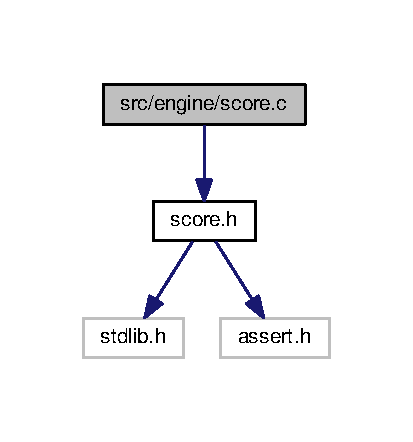
\includegraphics[width=198pt]{score_8c__incl}
\end{center}
\end{figure}
\subsection*{Functions}
\begin{DoxyCompactItemize}
\item 
unsigned int \textbf{ score\+\_\+compute\+\_\+break} (const int hist[$\,$], size\+\_\+t len, unsigned int level)
\end{DoxyCompactItemize}


\subsection{Detailed Description}
Scoring system. 

\begin{DoxyAuthor}{Author}
S4\+Master\+Race 
\end{DoxyAuthor}
\begin{DoxyVersion}{Version}
2.\+0 
\end{DoxyVersion}


\subsection{Function Documentation}
\mbox{\label{score_8c_a2879d92d899fcd81e056a304c03b3698}} 
\index{score.\+c@{score.\+c}!score\+\_\+compute\+\_\+break@{score\+\_\+compute\+\_\+break}}
\index{score\+\_\+compute\+\_\+break@{score\+\_\+compute\+\_\+break}!score.\+c@{score.\+c}}
\subsubsection{score\+\_\+compute\+\_\+break()}
{\footnotesize\ttfamily unsigned int score\+\_\+compute\+\_\+break (\begin{DoxyParamCaption}\item[{const int}]{hist[$\,$],  }\item[{size\+\_\+t}]{len,  }\item[{unsigned int}]{level }\end{DoxyParamCaption})}


\section{src/engine/score.h File Reference}
\label{score_8h}\index{src/engine/score.\+h@{src/engine/score.\+h}}


Scoring system.  


{\ttfamily \#include $<$stdlib.\+h$>$}\newline
{\ttfamily \#include $<$assert.\+h$>$}\newline
Include dependency graph for score.\+h\+:
\nopagebreak
\begin{figure}[H]
\begin{center}
\leavevmode
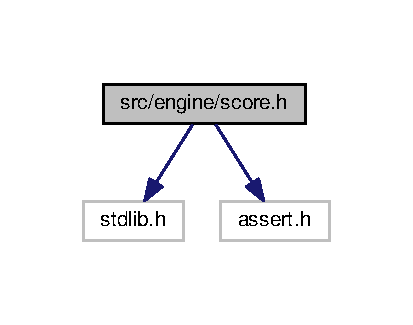
\includegraphics[width=198pt]{score_8h__incl}
\end{center}
\end{figure}
This graph shows which files directly or indirectly include this file\+:
\nopagebreak
\begin{figure}[H]
\begin{center}
\leavevmode
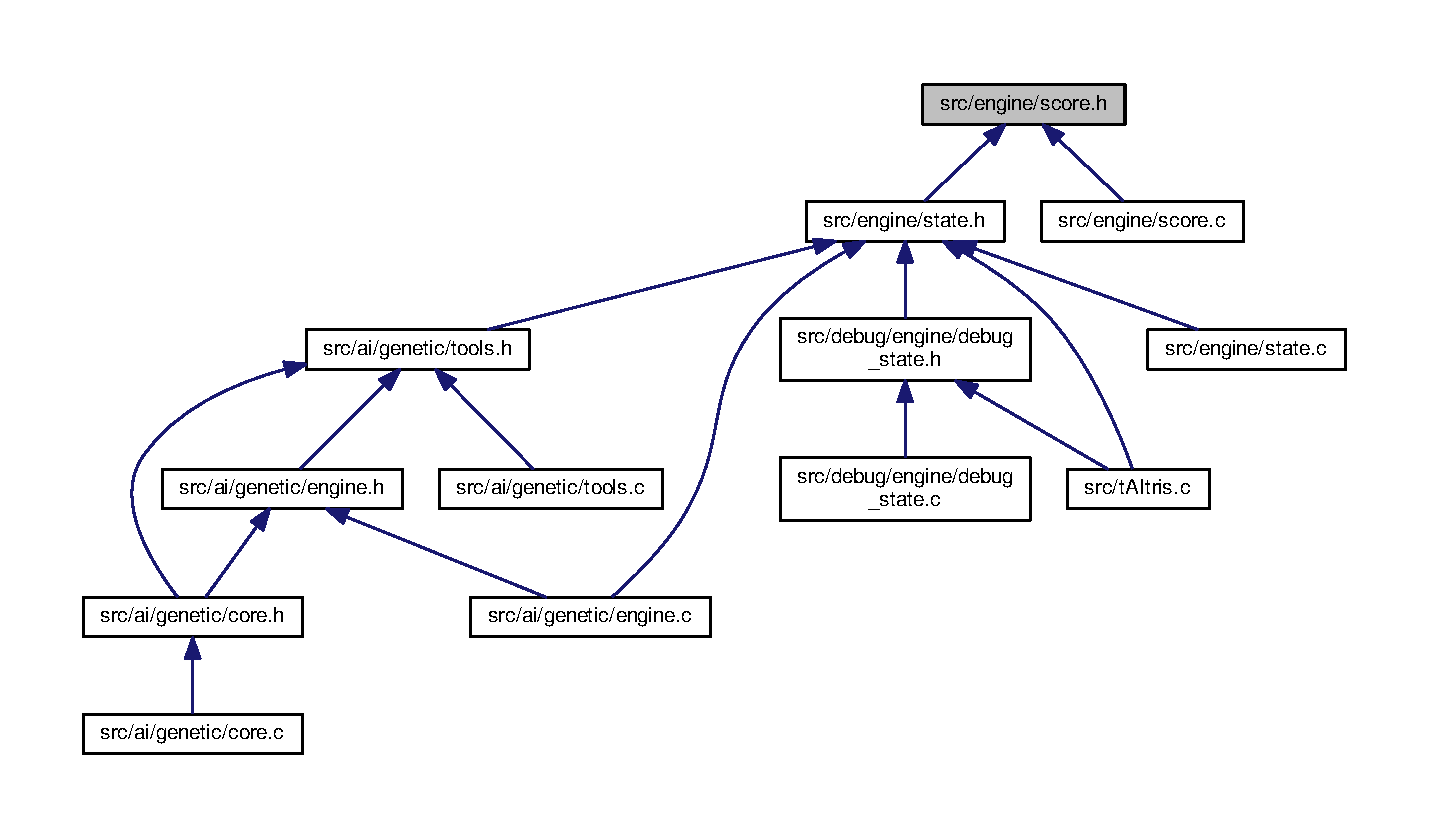
\includegraphics[width=350pt]{score_8h__dep__incl}
\end{center}
\end{figure}
\subsection*{Macros}
\begin{DoxyCompactItemize}
\item 
\#define \textbf{ S\+C\+O\+R\+E\+\_\+\+S\+I\+N\+G\+LE}~100
\item 
\#define \textbf{ S\+C\+O\+R\+E\+\_\+\+D\+O\+U\+B\+LE}~300
\item 
\#define \textbf{ S\+C\+O\+R\+E\+\_\+\+T\+R\+I\+P\+LE}~500
\item 
\#define \textbf{ S\+C\+O\+R\+E\+\_\+\+T\+E\+T\+R\+IS}~800
\item 
\#define \textbf{ S\+C\+O\+R\+E\+\_\+\+S\+D\+R\+OP}~1
\item 
\#define \textbf{ S\+C\+O\+R\+E\+\_\+\+H\+D\+R\+OP}~2
\end{DoxyCompactItemize}
\subsection*{Functions}
\begin{DoxyCompactItemize}
\item 
unsigned int \textbf{ score\+\_\+compute\+\_\+break} (const int hist[$\,$], size\+\_\+t len, unsigned int level)
\end{DoxyCompactItemize}


\subsection{Detailed Description}
Scoring system. 

\begin{DoxyAuthor}{Author}
S4\+Master\+Race 
\end{DoxyAuthor}
\begin{DoxyVersion}{Version}
2.\+0 
\end{DoxyVersion}


\subsection{Macro Definition Documentation}
\mbox{\label{score_8h_abf3a94c8c811229ec8c21ba8097f4a8f}} 
\index{score.\+h@{score.\+h}!S\+C\+O\+R\+E\+\_\+\+D\+O\+U\+B\+LE@{S\+C\+O\+R\+E\+\_\+\+D\+O\+U\+B\+LE}}
\index{S\+C\+O\+R\+E\+\_\+\+D\+O\+U\+B\+LE@{S\+C\+O\+R\+E\+\_\+\+D\+O\+U\+B\+LE}!score.\+h@{score.\+h}}
\subsubsection{S\+C\+O\+R\+E\+\_\+\+D\+O\+U\+B\+LE}
{\footnotesize\ttfamily \#define S\+C\+O\+R\+E\+\_\+\+D\+O\+U\+B\+LE~300}

\mbox{\label{score_8h_a21b90b04662b40af6aa45e9db2b005a1}} 
\index{score.\+h@{score.\+h}!S\+C\+O\+R\+E\+\_\+\+H\+D\+R\+OP@{S\+C\+O\+R\+E\+\_\+\+H\+D\+R\+OP}}
\index{S\+C\+O\+R\+E\+\_\+\+H\+D\+R\+OP@{S\+C\+O\+R\+E\+\_\+\+H\+D\+R\+OP}!score.\+h@{score.\+h}}
\subsubsection{S\+C\+O\+R\+E\+\_\+\+H\+D\+R\+OP}
{\footnotesize\ttfamily \#define S\+C\+O\+R\+E\+\_\+\+H\+D\+R\+OP~2}

\mbox{\label{score_8h_a1a58f663e89e5e3d71342ed0c26a865f}} 
\index{score.\+h@{score.\+h}!S\+C\+O\+R\+E\+\_\+\+S\+D\+R\+OP@{S\+C\+O\+R\+E\+\_\+\+S\+D\+R\+OP}}
\index{S\+C\+O\+R\+E\+\_\+\+S\+D\+R\+OP@{S\+C\+O\+R\+E\+\_\+\+S\+D\+R\+OP}!score.\+h@{score.\+h}}
\subsubsection{S\+C\+O\+R\+E\+\_\+\+S\+D\+R\+OP}
{\footnotesize\ttfamily \#define S\+C\+O\+R\+E\+\_\+\+S\+D\+R\+OP~1}

\mbox{\label{score_8h_aa4a6e169ddc7c2058e3ef7759008a695}} 
\index{score.\+h@{score.\+h}!S\+C\+O\+R\+E\+\_\+\+S\+I\+N\+G\+LE@{S\+C\+O\+R\+E\+\_\+\+S\+I\+N\+G\+LE}}
\index{S\+C\+O\+R\+E\+\_\+\+S\+I\+N\+G\+LE@{S\+C\+O\+R\+E\+\_\+\+S\+I\+N\+G\+LE}!score.\+h@{score.\+h}}
\subsubsection{S\+C\+O\+R\+E\+\_\+\+S\+I\+N\+G\+LE}
{\footnotesize\ttfamily \#define S\+C\+O\+R\+E\+\_\+\+S\+I\+N\+G\+LE~100}

\mbox{\label{score_8h_a5df0041655615401e0b0885839356aa5}} 
\index{score.\+h@{score.\+h}!S\+C\+O\+R\+E\+\_\+\+T\+E\+T\+R\+IS@{S\+C\+O\+R\+E\+\_\+\+T\+E\+T\+R\+IS}}
\index{S\+C\+O\+R\+E\+\_\+\+T\+E\+T\+R\+IS@{S\+C\+O\+R\+E\+\_\+\+T\+E\+T\+R\+IS}!score.\+h@{score.\+h}}
\subsubsection{S\+C\+O\+R\+E\+\_\+\+T\+E\+T\+R\+IS}
{\footnotesize\ttfamily \#define S\+C\+O\+R\+E\+\_\+\+T\+E\+T\+R\+IS~800}

\mbox{\label{score_8h_a48ce26ac27575c8cfe35effa16a22927}} 
\index{score.\+h@{score.\+h}!S\+C\+O\+R\+E\+\_\+\+T\+R\+I\+P\+LE@{S\+C\+O\+R\+E\+\_\+\+T\+R\+I\+P\+LE}}
\index{S\+C\+O\+R\+E\+\_\+\+T\+R\+I\+P\+LE@{S\+C\+O\+R\+E\+\_\+\+T\+R\+I\+P\+LE}!score.\+h@{score.\+h}}
\subsubsection{S\+C\+O\+R\+E\+\_\+\+T\+R\+I\+P\+LE}
{\footnotesize\ttfamily \#define S\+C\+O\+R\+E\+\_\+\+T\+R\+I\+P\+LE~500}



\subsection{Function Documentation}
\mbox{\label{score_8h_a2879d92d899fcd81e056a304c03b3698}} 
\index{score.\+h@{score.\+h}!score\+\_\+compute\+\_\+break@{score\+\_\+compute\+\_\+break}}
\index{score\+\_\+compute\+\_\+break@{score\+\_\+compute\+\_\+break}!score.\+h@{score.\+h}}
\subsubsection{score\+\_\+compute\+\_\+break()}
{\footnotesize\ttfamily unsigned int score\+\_\+compute\+\_\+break (\begin{DoxyParamCaption}\item[{const int}]{hist[$\,$],  }\item[{size\+\_\+t}]{len,  }\item[{unsigned int}]{level }\end{DoxyParamCaption})}


\section{src/engine/state.c File Reference}
\label{state_8c}\index{src/engine/state.\+c@{src/engine/state.\+c}}


\doxyref{State}{p.}{structState}.  


{\ttfamily \#include \char`\"{}state.\+h\char`\"{}}\newline
{\ttfamily \#include \char`\"{}board.\+h\char`\"{}}\newline
Include dependency graph for state.\+c\+:
\nopagebreak
\begin{figure}[H]
\begin{center}
\leavevmode
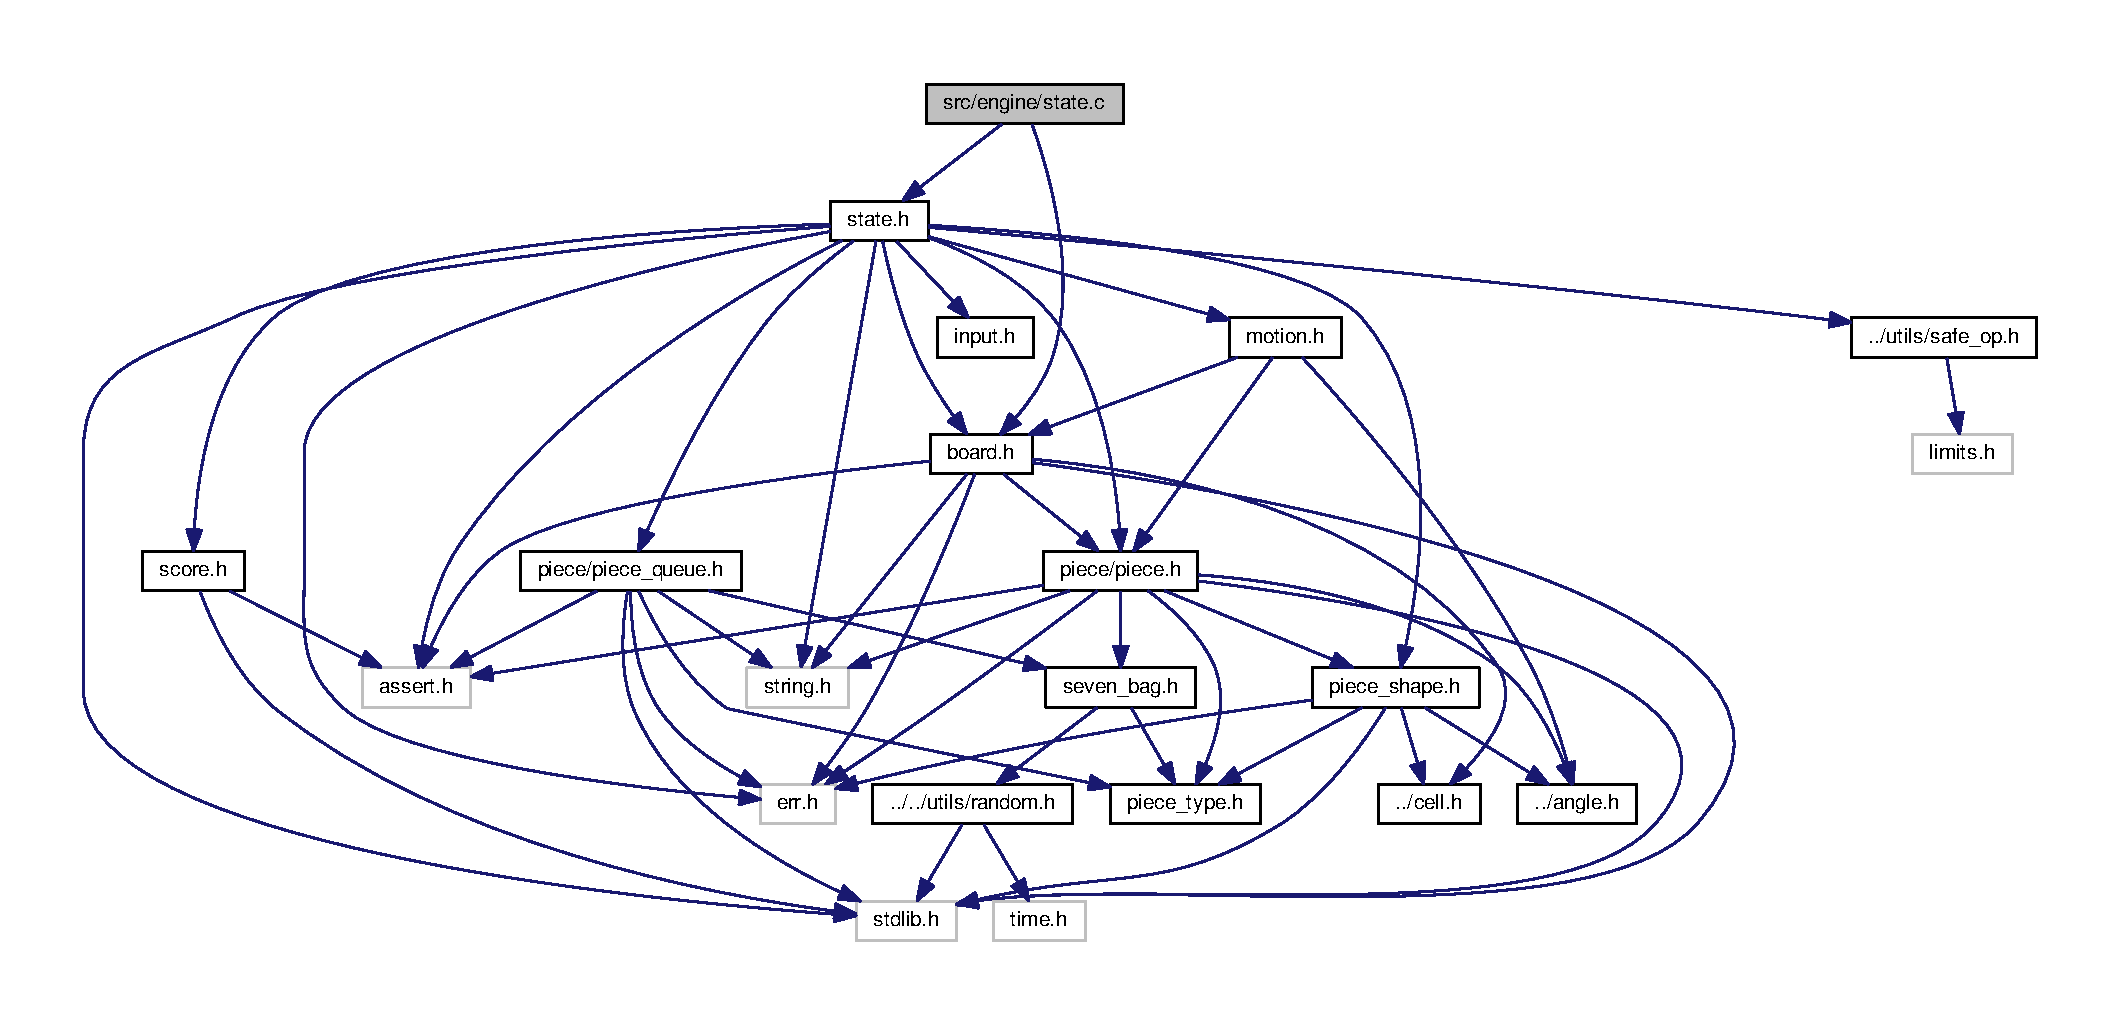
\includegraphics[width=350pt]{state_8c__incl}
\end{center}
\end{figure}
\subsection*{Functions}
\begin{DoxyCompactItemize}
\item 
\textbf{ State} $\ast$ \textbf{ state\+\_\+create} ()
\item 
void \textbf{ state\+\_\+init} (\textbf{ State} $\ast$state, \textbf{ Piece\+Queue} $\ast$q)
\item 
void \textbf{ state\+\_\+free} (\textbf{ State} $\ast$state)
\item 
\textbf{ State} $\ast$ \textbf{ state\+\_\+copy} (const \textbf{ State} $\ast$state)
\item 
\textbf{ Piece} $\ast$ \textbf{ state\+\_\+create\+\_\+piece} (\textbf{ State} $\ast$state)
\item 
void \textbf{ state\+\_\+next\+\_\+piece} (\textbf{ State} $\ast$state)
\item 
int \textbf{ state\+\_\+step} (\textbf{ State} $\ast$state)
\item 
int \textbf{ state\+\_\+apply\+\_\+input} (\textbf{ State} $\ast$state, \textbf{ Input} input)
\item 
int \textbf{ state\+\_\+apply\+\_\+inputs} (\textbf{ State} $\ast$state, \textbf{ Input} input[$\,$], size\+\_\+t len)
\item 
int \textbf{ state\+\_\+can\+\_\+apply\+\_\+input} (\textbf{ State} $\ast$state, \textbf{ Input} input)
\item 
int \textbf{ state\+\_\+can\+\_\+apply\+\_\+inputs} (\textbf{ State} $\ast$state, \textbf{ Input} input[$\,$], size\+\_\+t len)
\end{DoxyCompactItemize}


\subsection{Detailed Description}
\doxyref{State}{p.}{structState}. 

\begin{DoxyAuthor}{Author}
S4\+Master\+Race 
\end{DoxyAuthor}
\begin{DoxyVersion}{Version}
2.\+0 
\end{DoxyVersion}


\subsection{Function Documentation}
\mbox{\label{state_8c_ad93fdb98f5dc85b8fb3683e02631f369}} 
\index{state.\+c@{state.\+c}!state\+\_\+apply\+\_\+input@{state\+\_\+apply\+\_\+input}}
\index{state\+\_\+apply\+\_\+input@{state\+\_\+apply\+\_\+input}!state.\+c@{state.\+c}}
\subsubsection{state\+\_\+apply\+\_\+input()}
{\footnotesize\ttfamily int state\+\_\+apply\+\_\+input (\begin{DoxyParamCaption}\item[{\textbf{ State} $\ast$}]{state,  }\item[{\textbf{ Input}}]{input }\end{DoxyParamCaption})}

\mbox{\label{state_8c_ad1dbcd902c0cb09e397a59eea30de21b}} 
\index{state.\+c@{state.\+c}!state\+\_\+apply\+\_\+inputs@{state\+\_\+apply\+\_\+inputs}}
\index{state\+\_\+apply\+\_\+inputs@{state\+\_\+apply\+\_\+inputs}!state.\+c@{state.\+c}}
\subsubsection{state\+\_\+apply\+\_\+inputs()}
{\footnotesize\ttfamily int state\+\_\+apply\+\_\+inputs (\begin{DoxyParamCaption}\item[{\textbf{ State} $\ast$}]{state,  }\item[{\textbf{ Input}}]{input[$\,$],  }\item[{size\+\_\+t}]{len }\end{DoxyParamCaption})}

\mbox{\label{state_8c_ac4ed6442134df1ae3b4aae730290f6a3}} 
\index{state.\+c@{state.\+c}!state\+\_\+can\+\_\+apply\+\_\+input@{state\+\_\+can\+\_\+apply\+\_\+input}}
\index{state\+\_\+can\+\_\+apply\+\_\+input@{state\+\_\+can\+\_\+apply\+\_\+input}!state.\+c@{state.\+c}}
\subsubsection{state\+\_\+can\+\_\+apply\+\_\+input()}
{\footnotesize\ttfamily int state\+\_\+can\+\_\+apply\+\_\+input (\begin{DoxyParamCaption}\item[{\textbf{ State} $\ast$}]{state,  }\item[{\textbf{ Input}}]{input }\end{DoxyParamCaption})}

\mbox{\label{state_8c_a61a69f8f17434cec27e85e3f71cc0d89}} 
\index{state.\+c@{state.\+c}!state\+\_\+can\+\_\+apply\+\_\+inputs@{state\+\_\+can\+\_\+apply\+\_\+inputs}}
\index{state\+\_\+can\+\_\+apply\+\_\+inputs@{state\+\_\+can\+\_\+apply\+\_\+inputs}!state.\+c@{state.\+c}}
\subsubsection{state\+\_\+can\+\_\+apply\+\_\+inputs()}
{\footnotesize\ttfamily int state\+\_\+can\+\_\+apply\+\_\+inputs (\begin{DoxyParamCaption}\item[{\textbf{ State} $\ast$}]{state,  }\item[{\textbf{ Input}}]{input[$\,$],  }\item[{size\+\_\+t}]{len }\end{DoxyParamCaption})}

\mbox{\label{state_8c_addc44143a8bd40469bda8490abb37dfd}} 
\index{state.\+c@{state.\+c}!state\+\_\+copy@{state\+\_\+copy}}
\index{state\+\_\+copy@{state\+\_\+copy}!state.\+c@{state.\+c}}
\subsubsection{state\+\_\+copy()}
{\footnotesize\ttfamily \textbf{ State}$\ast$ state\+\_\+copy (\begin{DoxyParamCaption}\item[{const \textbf{ State} $\ast$}]{state }\end{DoxyParamCaption})}

\mbox{\label{state_8c_a062a4e5de219642b719e52a9e23e9abc}} 
\index{state.\+c@{state.\+c}!state\+\_\+create@{state\+\_\+create}}
\index{state\+\_\+create@{state\+\_\+create}!state.\+c@{state.\+c}}
\subsubsection{state\+\_\+create()}
{\footnotesize\ttfamily \textbf{ State}$\ast$ state\+\_\+create (\begin{DoxyParamCaption}{ }\end{DoxyParamCaption})}

\mbox{\label{state_8c_a9ce2081e85b17a281b25cd633342edf5}} 
\index{state.\+c@{state.\+c}!state\+\_\+create\+\_\+piece@{state\+\_\+create\+\_\+piece}}
\index{state\+\_\+create\+\_\+piece@{state\+\_\+create\+\_\+piece}!state.\+c@{state.\+c}}
\subsubsection{state\+\_\+create\+\_\+piece()}
{\footnotesize\ttfamily \textbf{ Piece}$\ast$ state\+\_\+create\+\_\+piece (\begin{DoxyParamCaption}\item[{\textbf{ State} $\ast$}]{state }\end{DoxyParamCaption})}

\mbox{\label{state_8c_a8c884ea08b83339c02525c6b581d4448}} 
\index{state.\+c@{state.\+c}!state\+\_\+free@{state\+\_\+free}}
\index{state\+\_\+free@{state\+\_\+free}!state.\+c@{state.\+c}}
\subsubsection{state\+\_\+free()}
{\footnotesize\ttfamily void state\+\_\+free (\begin{DoxyParamCaption}\item[{\textbf{ State} $\ast$}]{state }\end{DoxyParamCaption})}

\mbox{\label{state_8c_adcb5cdc65623cbd0d6d073eb5c8f7e1f}} 
\index{state.\+c@{state.\+c}!state\+\_\+init@{state\+\_\+init}}
\index{state\+\_\+init@{state\+\_\+init}!state.\+c@{state.\+c}}
\subsubsection{state\+\_\+init()}
{\footnotesize\ttfamily void state\+\_\+init (\begin{DoxyParamCaption}\item[{\textbf{ State} $\ast$}]{state,  }\item[{\textbf{ Piece\+Queue} $\ast$}]{q }\end{DoxyParamCaption})}

\mbox{\label{state_8c_a5f417880078be22e9de4ef37ad5d692d}} 
\index{state.\+c@{state.\+c}!state\+\_\+next\+\_\+piece@{state\+\_\+next\+\_\+piece}}
\index{state\+\_\+next\+\_\+piece@{state\+\_\+next\+\_\+piece}!state.\+c@{state.\+c}}
\subsubsection{state\+\_\+next\+\_\+piece()}
{\footnotesize\ttfamily void state\+\_\+next\+\_\+piece (\begin{DoxyParamCaption}\item[{\textbf{ State} $\ast$}]{state }\end{DoxyParamCaption})}

\mbox{\label{state_8c_a1975f06362a2e02c66671595393bedcd}} 
\index{state.\+c@{state.\+c}!state\+\_\+step@{state\+\_\+step}}
\index{state\+\_\+step@{state\+\_\+step}!state.\+c@{state.\+c}}
\subsubsection{state\+\_\+step()}
{\footnotesize\ttfamily int state\+\_\+step (\begin{DoxyParamCaption}\item[{\textbf{ State} $\ast$}]{state }\end{DoxyParamCaption})}


\section{src/engine/state.h File Reference}
\label{state_8h}\index{src/engine/state.\+h@{src/engine/state.\+h}}


\doxyref{State}{p.}{structState}.  


{\ttfamily \#include $<$stdlib.\+h$>$}\newline
{\ttfamily \#include $<$err.\+h$>$}\newline
{\ttfamily \#include $<$string.\+h$>$}\newline
{\ttfamily \#include $<$assert.\+h$>$}\newline
{\ttfamily \#include \char`\"{}board.\+h\char`\"{}}\newline
{\ttfamily \#include \char`\"{}piece/piece.\+h\char`\"{}}\newline
{\ttfamily \#include \char`\"{}piece/piece\+\_\+shape.\+h\char`\"{}}\newline
{\ttfamily \#include \char`\"{}piece/piece\+\_\+queue.\+h\char`\"{}}\newline
{\ttfamily \#include \char`\"{}motion.\+h\char`\"{}}\newline
{\ttfamily \#include \char`\"{}input.\+h\char`\"{}}\newline
{\ttfamily \#include \char`\"{}score.\+h\char`\"{}}\newline
{\ttfamily \#include \char`\"{}../utils/safe\+\_\+op.\+h\char`\"{}}\newline
Include dependency graph for state.\+h\+:
\nopagebreak
\begin{figure}[H]
\begin{center}
\leavevmode
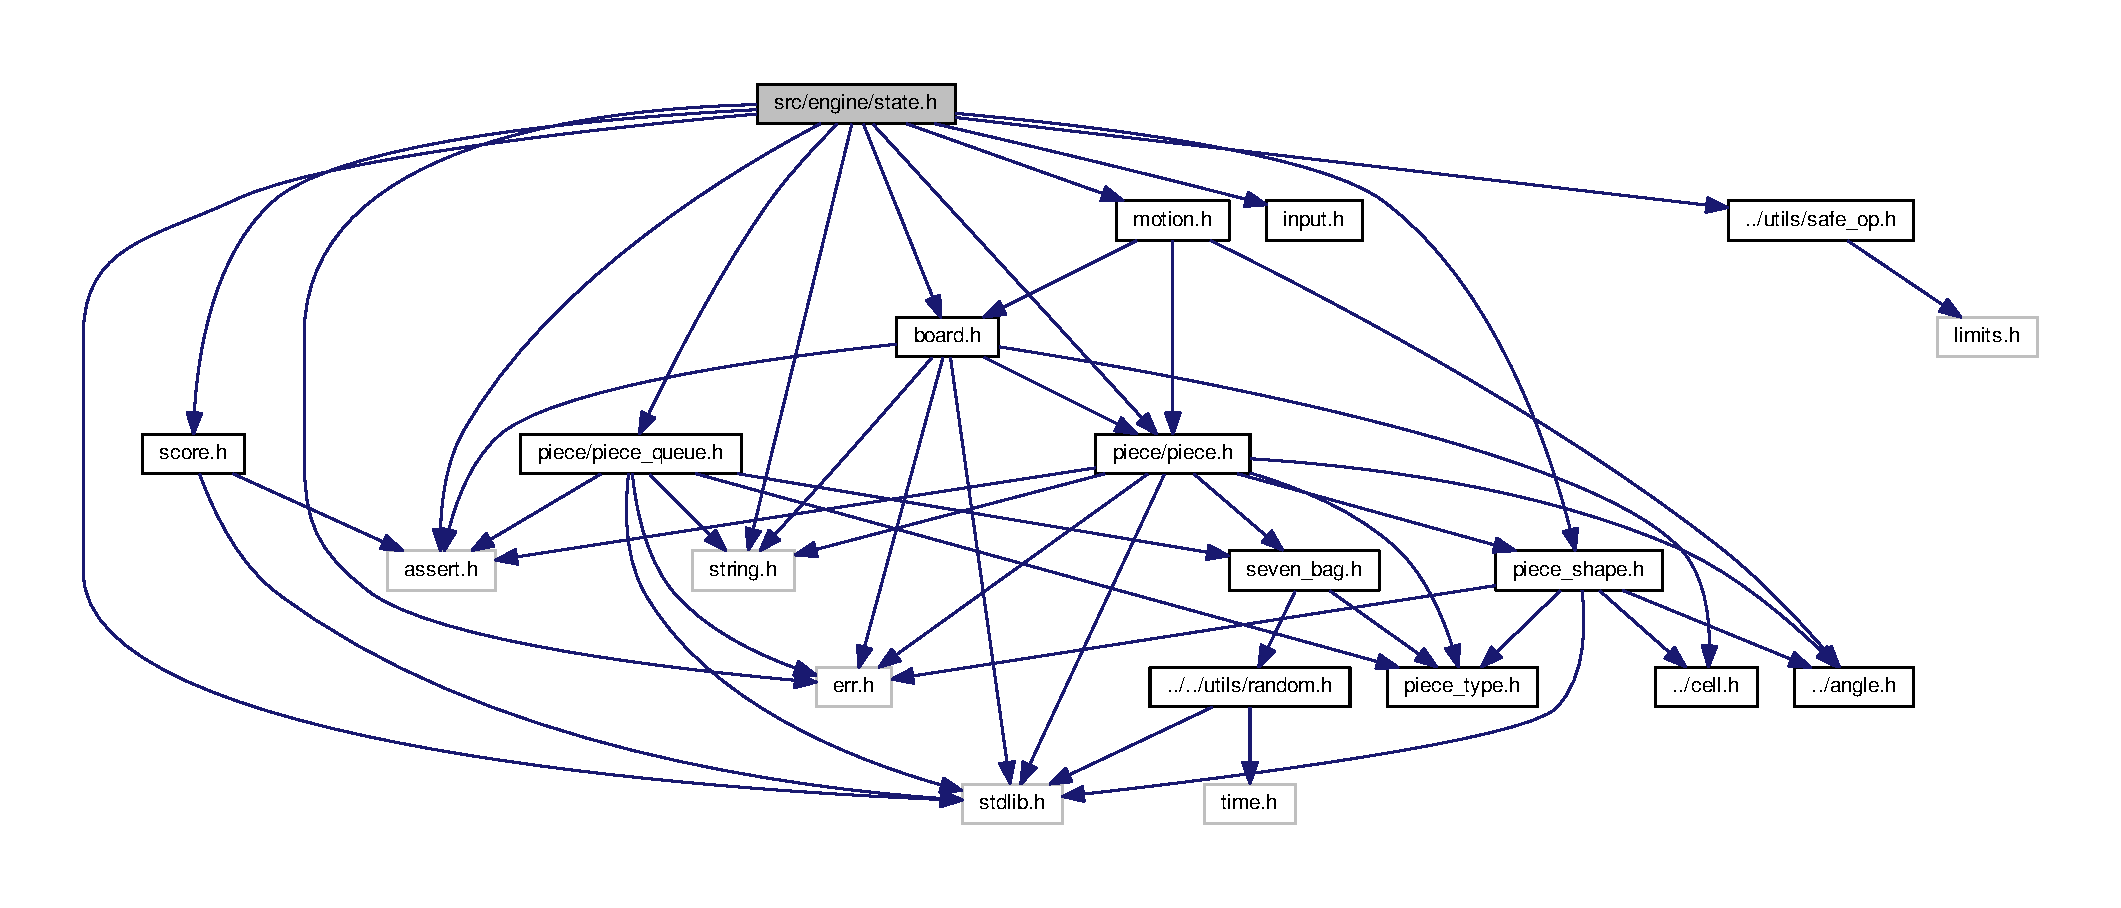
\includegraphics[width=350pt]{state_8h__incl}
\end{center}
\end{figure}
This graph shows which files directly or indirectly include this file\+:
\nopagebreak
\begin{figure}[H]
\begin{center}
\leavevmode
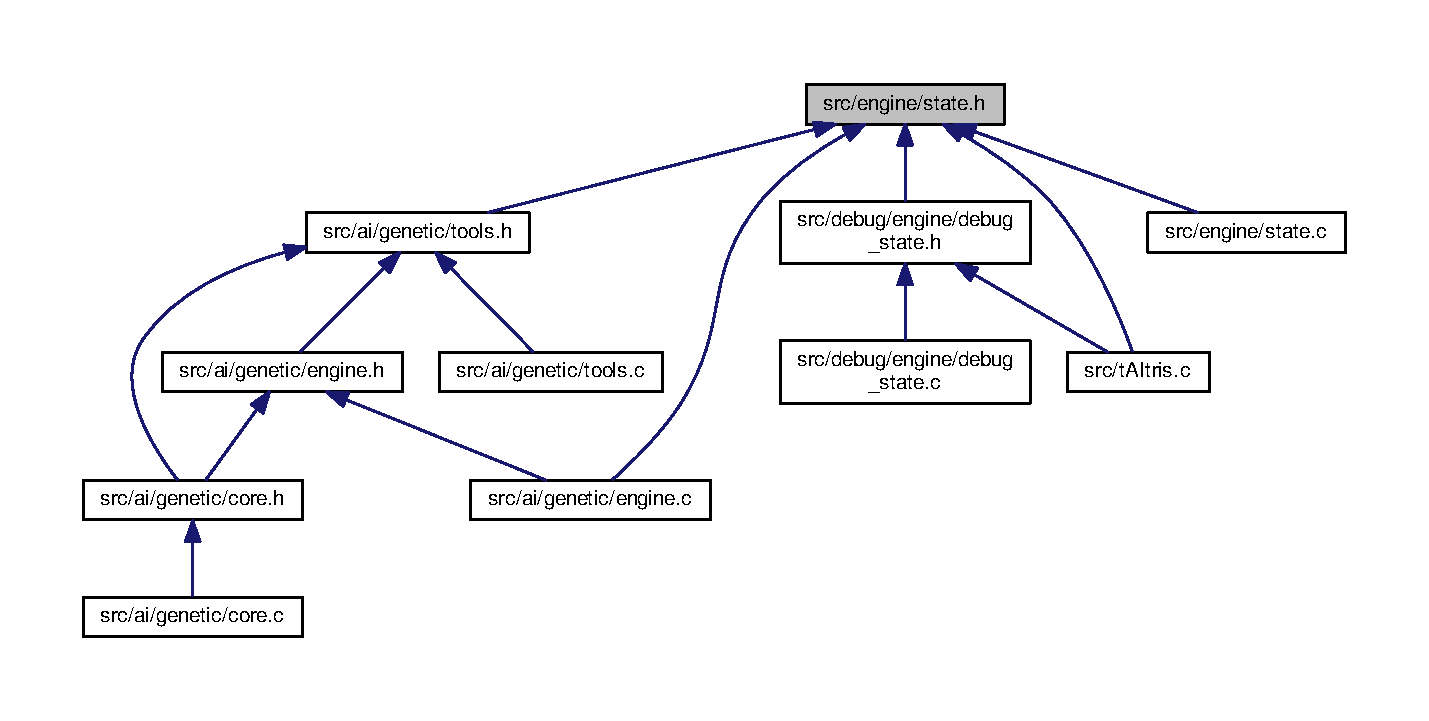
\includegraphics[width=350pt]{state_8h__dep__incl}
\end{center}
\end{figure}
\subsection*{Data Structures}
\begin{DoxyCompactItemize}
\item 
struct \textbf{ State}
\end{DoxyCompactItemize}
\subsection*{Functions}
\begin{DoxyCompactItemize}
\item 
\textbf{ State} $\ast$ \textbf{ state\+\_\+create} ()
\item 
void \textbf{ state\+\_\+init} (\textbf{ State} $\ast$state, \textbf{ Piece\+Queue} $\ast$q)
\item 
void \textbf{ state\+\_\+free} (\textbf{ State} $\ast$state)
\item 
\textbf{ State} $\ast$ \textbf{ state\+\_\+copy} (const \textbf{ State} $\ast$state)
\item 
\textbf{ Piece} $\ast$ \textbf{ state\+\_\+create\+\_\+piece} (\textbf{ State} $\ast$state)
\item 
void \textbf{ state\+\_\+next\+\_\+piece} (\textbf{ State} $\ast$state)
\item 
int \textbf{ state\+\_\+step} (\textbf{ State} $\ast$state)
\item 
int \textbf{ state\+\_\+apply\+\_\+input} (\textbf{ State} $\ast$state, \textbf{ Input} input)
\item 
int \textbf{ state\+\_\+apply\+\_\+inputs} (\textbf{ State} $\ast$state, \textbf{ Input} input[$\,$], size\+\_\+t len)
\item 
int \textbf{ state\+\_\+can\+\_\+apply\+\_\+input} (\textbf{ State} $\ast$state, \textbf{ Input} input)
\item 
int \textbf{ state\+\_\+can\+\_\+apply\+\_\+inputs} (\textbf{ State} $\ast$state, \textbf{ Input} input[$\,$], size\+\_\+t len)
\end{DoxyCompactItemize}


\subsection{Detailed Description}
\doxyref{State}{p.}{structState}. 

\begin{DoxyAuthor}{Author}
S4\+Master\+Race 
\end{DoxyAuthor}
\begin{DoxyVersion}{Version}
2.\+0 
\end{DoxyVersion}


\subsection{Function Documentation}
\mbox{\label{state_8h_ad93fdb98f5dc85b8fb3683e02631f369}} 
\index{state.\+h@{state.\+h}!state\+\_\+apply\+\_\+input@{state\+\_\+apply\+\_\+input}}
\index{state\+\_\+apply\+\_\+input@{state\+\_\+apply\+\_\+input}!state.\+h@{state.\+h}}
\subsubsection{state\+\_\+apply\+\_\+input()}
{\footnotesize\ttfamily int state\+\_\+apply\+\_\+input (\begin{DoxyParamCaption}\item[{\textbf{ State} $\ast$}]{state,  }\item[{\textbf{ Input}}]{input }\end{DoxyParamCaption})}

\mbox{\label{state_8h_ad1dbcd902c0cb09e397a59eea30de21b}} 
\index{state.\+h@{state.\+h}!state\+\_\+apply\+\_\+inputs@{state\+\_\+apply\+\_\+inputs}}
\index{state\+\_\+apply\+\_\+inputs@{state\+\_\+apply\+\_\+inputs}!state.\+h@{state.\+h}}
\subsubsection{state\+\_\+apply\+\_\+inputs()}
{\footnotesize\ttfamily int state\+\_\+apply\+\_\+inputs (\begin{DoxyParamCaption}\item[{\textbf{ State} $\ast$}]{state,  }\item[{\textbf{ Input}}]{input[$\,$],  }\item[{size\+\_\+t}]{len }\end{DoxyParamCaption})}

\mbox{\label{state_8h_ac4ed6442134df1ae3b4aae730290f6a3}} 
\index{state.\+h@{state.\+h}!state\+\_\+can\+\_\+apply\+\_\+input@{state\+\_\+can\+\_\+apply\+\_\+input}}
\index{state\+\_\+can\+\_\+apply\+\_\+input@{state\+\_\+can\+\_\+apply\+\_\+input}!state.\+h@{state.\+h}}
\subsubsection{state\+\_\+can\+\_\+apply\+\_\+input()}
{\footnotesize\ttfamily int state\+\_\+can\+\_\+apply\+\_\+input (\begin{DoxyParamCaption}\item[{\textbf{ State} $\ast$}]{state,  }\item[{\textbf{ Input}}]{input }\end{DoxyParamCaption})}

\mbox{\label{state_8h_a61a69f8f17434cec27e85e3f71cc0d89}} 
\index{state.\+h@{state.\+h}!state\+\_\+can\+\_\+apply\+\_\+inputs@{state\+\_\+can\+\_\+apply\+\_\+inputs}}
\index{state\+\_\+can\+\_\+apply\+\_\+inputs@{state\+\_\+can\+\_\+apply\+\_\+inputs}!state.\+h@{state.\+h}}
\subsubsection{state\+\_\+can\+\_\+apply\+\_\+inputs()}
{\footnotesize\ttfamily int state\+\_\+can\+\_\+apply\+\_\+inputs (\begin{DoxyParamCaption}\item[{\textbf{ State} $\ast$}]{state,  }\item[{\textbf{ Input}}]{input[$\,$],  }\item[{size\+\_\+t}]{len }\end{DoxyParamCaption})}

\mbox{\label{state_8h_addc44143a8bd40469bda8490abb37dfd}} 
\index{state.\+h@{state.\+h}!state\+\_\+copy@{state\+\_\+copy}}
\index{state\+\_\+copy@{state\+\_\+copy}!state.\+h@{state.\+h}}
\subsubsection{state\+\_\+copy()}
{\footnotesize\ttfamily \textbf{ State}$\ast$ state\+\_\+copy (\begin{DoxyParamCaption}\item[{const \textbf{ State} $\ast$}]{state }\end{DoxyParamCaption})}

\mbox{\label{state_8h_a062a4e5de219642b719e52a9e23e9abc}} 
\index{state.\+h@{state.\+h}!state\+\_\+create@{state\+\_\+create}}
\index{state\+\_\+create@{state\+\_\+create}!state.\+h@{state.\+h}}
\subsubsection{state\+\_\+create()}
{\footnotesize\ttfamily \textbf{ State}$\ast$ state\+\_\+create (\begin{DoxyParamCaption}{ }\end{DoxyParamCaption})}

\mbox{\label{state_8h_a9ce2081e85b17a281b25cd633342edf5}} 
\index{state.\+h@{state.\+h}!state\+\_\+create\+\_\+piece@{state\+\_\+create\+\_\+piece}}
\index{state\+\_\+create\+\_\+piece@{state\+\_\+create\+\_\+piece}!state.\+h@{state.\+h}}
\subsubsection{state\+\_\+create\+\_\+piece()}
{\footnotesize\ttfamily \textbf{ Piece}$\ast$ state\+\_\+create\+\_\+piece (\begin{DoxyParamCaption}\item[{\textbf{ State} $\ast$}]{state }\end{DoxyParamCaption})}

\mbox{\label{state_8h_a8c884ea08b83339c02525c6b581d4448}} 
\index{state.\+h@{state.\+h}!state\+\_\+free@{state\+\_\+free}}
\index{state\+\_\+free@{state\+\_\+free}!state.\+h@{state.\+h}}
\subsubsection{state\+\_\+free()}
{\footnotesize\ttfamily void state\+\_\+free (\begin{DoxyParamCaption}\item[{\textbf{ State} $\ast$}]{state }\end{DoxyParamCaption})}

\mbox{\label{state_8h_adcb5cdc65623cbd0d6d073eb5c8f7e1f}} 
\index{state.\+h@{state.\+h}!state\+\_\+init@{state\+\_\+init}}
\index{state\+\_\+init@{state\+\_\+init}!state.\+h@{state.\+h}}
\subsubsection{state\+\_\+init()}
{\footnotesize\ttfamily void state\+\_\+init (\begin{DoxyParamCaption}\item[{\textbf{ State} $\ast$}]{state,  }\item[{\textbf{ Piece\+Queue} $\ast$}]{q }\end{DoxyParamCaption})}

\mbox{\label{state_8h_a5f417880078be22e9de4ef37ad5d692d}} 
\index{state.\+h@{state.\+h}!state\+\_\+next\+\_\+piece@{state\+\_\+next\+\_\+piece}}
\index{state\+\_\+next\+\_\+piece@{state\+\_\+next\+\_\+piece}!state.\+h@{state.\+h}}
\subsubsection{state\+\_\+next\+\_\+piece()}
{\footnotesize\ttfamily void state\+\_\+next\+\_\+piece (\begin{DoxyParamCaption}\item[{\textbf{ State} $\ast$}]{state }\end{DoxyParamCaption})}

\mbox{\label{state_8h_a1975f06362a2e02c66671595393bedcd}} 
\index{state.\+h@{state.\+h}!state\+\_\+step@{state\+\_\+step}}
\index{state\+\_\+step@{state\+\_\+step}!state.\+h@{state.\+h}}
\subsubsection{state\+\_\+step()}
{\footnotesize\ttfamily int state\+\_\+step (\begin{DoxyParamCaption}\item[{\textbf{ State} $\ast$}]{state }\end{DoxyParamCaption})}


\section{src/t\+A\+Itris.c File Reference}
\label{tAItris_8c}\index{src/t\+A\+Itris.\+c@{src/t\+A\+Itris.\+c}}


Main file.  


{\ttfamily \#include \char`\"{}utils/random.\+h\char`\"{}}\newline
{\ttfamily \#include \char`\"{}engine/piece/piece\+\_\+queue.\+h\char`\"{}}\newline
{\ttfamily \#include \char`\"{}engine/state.\+h\char`\"{}}\newline
{\ttfamily \#include \char`\"{}debug/engine/debug\+\_\+state.\+h\char`\"{}}\newline
Include dependency graph for t\+A\+Itris.\+c\+:
\nopagebreak
\begin{figure}[H]
\begin{center}
\leavevmode
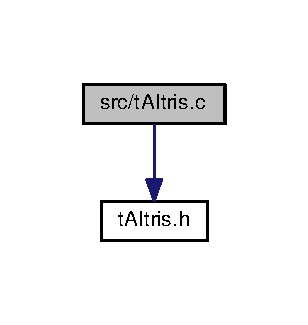
\includegraphics[width=350pt]{tAItris_8c__incl}
\end{center}
\end{figure}
\subsection*{Functions}
\begin{DoxyCompactItemize}
\item 
int \textbf{ main} ()
\end{DoxyCompactItemize}


\subsection{Detailed Description}
Main file. 

\begin{DoxyAuthor}{Author}
S4\+Master\+Race 
\end{DoxyAuthor}
\begin{DoxyVersion}{Version}
2.\+0 
\end{DoxyVersion}


\subsection{Function Documentation}
\mbox{\label{tAItris_8c_ae66f6b31b5ad750f1fe042a706a4e3d4}} 
\index{t\+A\+Itris.\+c@{t\+A\+Itris.\+c}!main@{main}}
\index{main@{main}!t\+A\+Itris.\+c@{t\+A\+Itris.\+c}}
\subsubsection{main()}
{\footnotesize\ttfamily int main (\begin{DoxyParamCaption}{ }\end{DoxyParamCaption})}


\section{src/utils/ansi\+\_\+code.h File Reference}
\label{ansi__code_8h}\index{src/utils/ansi\+\_\+code.\+h@{src/utils/ansi\+\_\+code.\+h}}


A\+N\+SI escape code.  


This graph shows which files directly or indirectly include this file\+:
\nopagebreak
\begin{figure}[H]
\begin{center}
\leavevmode
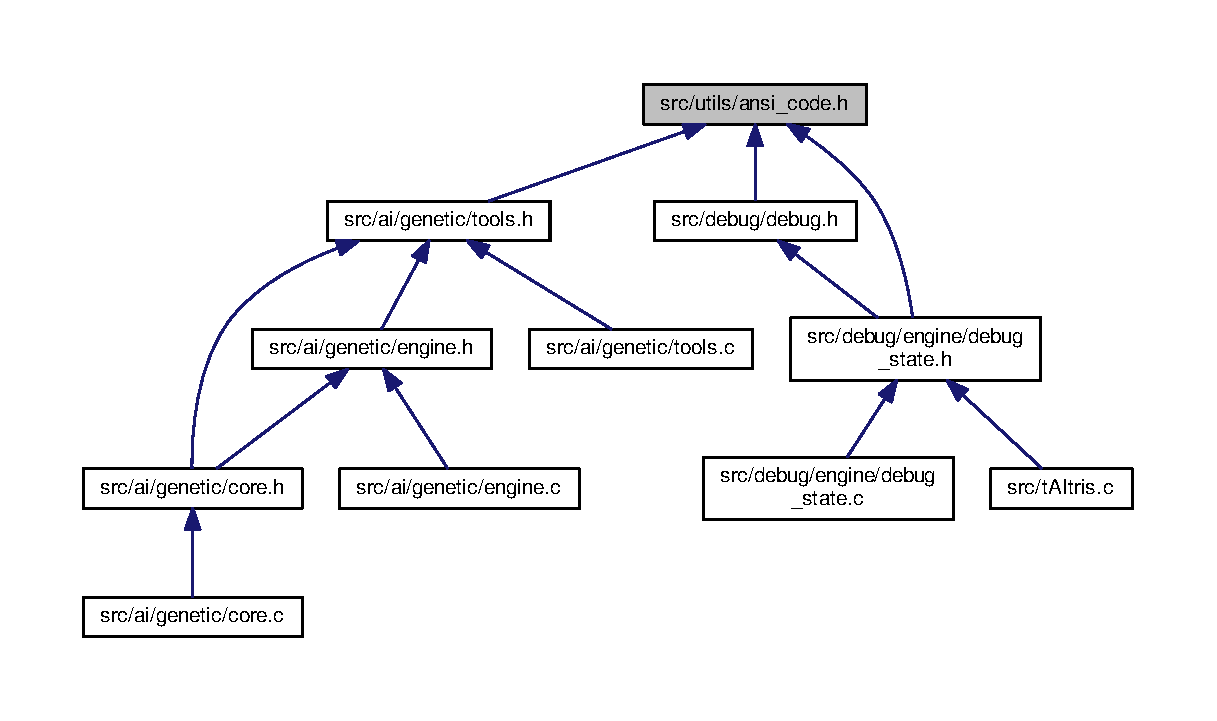
\includegraphics[width=350pt]{ansi__code_8h__dep__incl}
\end{center}
\end{figure}
\subsection*{Macros}
\begin{DoxyCompactItemize}
\item 
\#define \textbf{ A\+N\+S\+I\+\_\+\+E\+SC}~\char`\"{}\textbackslash{}x1b\char`\"{}
\item 
\#define \textbf{ A\+N\+S\+I\+\_\+\+S\+GR}(\+\_\+code\+\_\+)~\textbf{ A\+N\+S\+I\+\_\+\+E\+SC} \char`\"{}[\char`\"{} \#\+\_\+code\+\_\+ \char`\"{}m\char`\"{}
\item 
\#define \textbf{ A\+N\+S\+I\+\_\+\+R\+E\+S\+ET}~\textbf{ A\+N\+S\+I\+\_\+\+S\+GR}(0)
\item 
\#define \textbf{ A\+N\+S\+I\+\_\+\+B\+O\+LD}~\textbf{ A\+N\+S\+I\+\_\+\+S\+GR}(1)
\item 
\#define \textbf{ A\+N\+S\+I\+\_\+\+F\+A\+I\+NT}~\textbf{ A\+N\+S\+I\+\_\+\+S\+GR}(2)
\item 
\#define \textbf{ A\+N\+S\+I\+\_\+\+I\+T\+A\+L\+IC}~\textbf{ A\+N\+S\+I\+\_\+\+S\+GR}(3)
\item 
\#define \textbf{ A\+N\+S\+I\+\_\+\+U\+N\+D\+E\+R\+L\+I\+NE}~\textbf{ A\+N\+S\+I\+\_\+\+S\+GR}(4)
\item 
\#define \textbf{ A\+N\+S\+I\+\_\+\+S\+B\+L\+I\+NK}~\textbf{ A\+N\+S\+I\+\_\+\+S\+GR}(5)
\item 
\#define \textbf{ A\+N\+S\+I\+\_\+\+R\+B\+L\+I\+NK}~\textbf{ A\+N\+S\+I\+\_\+\+S\+GR}(6)
\item 
\#define \textbf{ A\+N\+S\+I\+\_\+\+C\+R\+O\+S\+S\+E\+D\+O\+UT}~\textbf{ A\+N\+S\+I\+\_\+\+S\+GR}(9)
\item 
\#define \textbf{ A\+N\+S\+I\+\_\+\+F\+R\+A\+M\+ED}~\textbf{ A\+N\+S\+I\+\_\+\+S\+GR}(51)
\item 
\#define \textbf{ A\+N\+S\+I\+\_\+\+E\+N\+C\+I\+R\+C\+L\+ED}~\textbf{ A\+N\+S\+I\+\_\+\+S\+GR}(52)
\item 
\#define \textbf{ A\+N\+S\+I\+\_\+\+O\+V\+E\+R\+L\+I\+N\+ED}~\textbf{ A\+N\+S\+I\+\_\+\+S\+GR}(53)
\item 
\#define \textbf{ A\+N\+S\+I\+\_\+\+F\+G\+\_\+\+D\+E\+F\+A\+U\+LT}~\textbf{ A\+N\+S\+I\+\_\+\+S\+GR}(39)
\item 
\#define \textbf{ A\+N\+S\+I\+\_\+\+F\+G\+\_\+\+B\+L\+A\+CK}~\textbf{ A\+N\+S\+I\+\_\+\+S\+GR}(30)
\item 
\#define \textbf{ A\+N\+S\+I\+\_\+\+F\+G\+\_\+\+R\+ED}~\textbf{ A\+N\+S\+I\+\_\+\+S\+GR}(31)
\item 
\#define \textbf{ A\+N\+S\+I\+\_\+\+F\+G\+\_\+\+G\+R\+E\+EN}~\textbf{ A\+N\+S\+I\+\_\+\+S\+GR}(32)
\item 
\#define \textbf{ A\+N\+S\+I\+\_\+\+F\+G\+\_\+\+Y\+E\+L\+L\+OW}~\textbf{ A\+N\+S\+I\+\_\+\+S\+GR}(33)
\item 
\#define \textbf{ A\+N\+S\+I\+\_\+\+F\+G\+\_\+\+B\+L\+UE}~\textbf{ A\+N\+S\+I\+\_\+\+S\+GR}(34)
\item 
\#define \textbf{ A\+N\+S\+I\+\_\+\+F\+G\+\_\+\+M\+A\+G\+E\+N\+TA}~\textbf{ A\+N\+S\+I\+\_\+\+S\+GR}(35)
\item 
\#define \textbf{ A\+N\+S\+I\+\_\+\+F\+G\+\_\+\+C\+Y\+AN}~\textbf{ A\+N\+S\+I\+\_\+\+S\+GR}(36)
\item 
\#define \textbf{ A\+N\+S\+I\+\_\+\+F\+G\+\_\+\+W\+H\+I\+TE}~\textbf{ A\+N\+S\+I\+\_\+\+S\+GR}(37)
\item 
\#define \textbf{ A\+N\+S\+I\+\_\+\+F\+G\+\_\+\+B\+B\+L\+A\+CK}~\textbf{ A\+N\+S\+I\+\_\+\+S\+GR}(90)
\item 
\#define \textbf{ A\+N\+S\+I\+\_\+\+F\+G\+\_\+\+B\+R\+ED}~\textbf{ A\+N\+S\+I\+\_\+\+S\+GR}(91)
\item 
\#define \textbf{ A\+N\+S\+I\+\_\+\+F\+G\+\_\+\+B\+G\+R\+E\+EN}~\textbf{ A\+N\+S\+I\+\_\+\+S\+GR}(92)
\item 
\#define \textbf{ A\+N\+S\+I\+\_\+\+F\+G\+\_\+\+B\+Y\+E\+L\+L\+OW}~\textbf{ A\+N\+S\+I\+\_\+\+S\+GR}(93)
\item 
\#define \textbf{ A\+N\+S\+I\+\_\+\+F\+G\+\_\+\+B\+B\+L\+UE}~\textbf{ A\+N\+S\+I\+\_\+\+S\+GR}(94)
\item 
\#define \textbf{ A\+N\+S\+I\+\_\+\+F\+G\+\_\+\+B\+M\+A\+G\+E\+N\+TA}~\textbf{ A\+N\+S\+I\+\_\+\+S\+GR}(95)
\item 
\#define \textbf{ A\+N\+S\+I\+\_\+\+F\+G\+\_\+\+B\+C\+Y\+AN}~\textbf{ A\+N\+S\+I\+\_\+\+S\+GR}(96)
\item 
\#define \textbf{ A\+N\+S\+I\+\_\+\+F\+G\+\_\+\+B\+W\+H\+I\+TE}~\textbf{ A\+N\+S\+I\+\_\+\+S\+GR}(97)
\item 
\#define \textbf{ A\+N\+S\+I\+\_\+\+B\+G\+\_\+\+D\+E\+F\+A\+U\+LT}~\textbf{ A\+N\+S\+I\+\_\+\+S\+GR}(49)
\item 
\#define \textbf{ A\+N\+S\+I\+\_\+\+B\+G\+\_\+\+B\+L\+A\+CK}~\textbf{ A\+N\+S\+I\+\_\+\+S\+GR}(40)
\item 
\#define \textbf{ A\+N\+S\+I\+\_\+\+B\+G\+\_\+\+R\+ED}~\textbf{ A\+N\+S\+I\+\_\+\+S\+GR}(41)
\item 
\#define \textbf{ A\+N\+S\+I\+\_\+\+B\+G\+\_\+\+G\+R\+E\+EN}~\textbf{ A\+N\+S\+I\+\_\+\+S\+GR}(42)
\item 
\#define \textbf{ A\+N\+S\+I\+\_\+\+B\+G\+\_\+\+Y\+E\+L\+L\+OW}~\textbf{ A\+N\+S\+I\+\_\+\+S\+GR}(43)
\item 
\#define \textbf{ A\+N\+S\+I\+\_\+\+B\+G\+\_\+\+B\+L\+UE}~\textbf{ A\+N\+S\+I\+\_\+\+S\+GR}(44)
\item 
\#define \textbf{ A\+N\+S\+I\+\_\+\+B\+G\+\_\+\+M\+A\+G\+E\+N\+TA}~\textbf{ A\+N\+S\+I\+\_\+\+S\+GR}(45)
\item 
\#define \textbf{ A\+N\+S\+I\+\_\+\+B\+G\+\_\+\+C\+Y\+AN}~\textbf{ A\+N\+S\+I\+\_\+\+S\+GR}(46)
\item 
\#define \textbf{ A\+N\+S\+I\+\_\+\+B\+G\+\_\+\+W\+H\+I\+TE}~\textbf{ A\+N\+S\+I\+\_\+\+S\+GR}(47)
\item 
\#define \textbf{ A\+N\+S\+I\+\_\+\+B\+G\+\_\+\+B\+B\+L\+A\+CK}~\textbf{ A\+N\+S\+I\+\_\+\+S\+GR}(100)
\item 
\#define \textbf{ A\+N\+S\+I\+\_\+\+B\+G\+\_\+\+B\+R\+ED}~\textbf{ A\+N\+S\+I\+\_\+\+S\+GR}(101)
\item 
\#define \textbf{ A\+N\+S\+I\+\_\+\+B\+G\+\_\+\+B\+G\+R\+E\+EN}~\textbf{ A\+N\+S\+I\+\_\+\+S\+GR}(102)
\item 
\#define \textbf{ A\+N\+S\+I\+\_\+\+B\+G\+\_\+\+B\+Y\+E\+L\+L\+OW}~\textbf{ A\+N\+S\+I\+\_\+\+S\+GR}(103)
\item 
\#define \textbf{ A\+N\+S\+I\+\_\+\+B\+G\+\_\+\+B\+B\+L\+UE}~\textbf{ A\+N\+S\+I\+\_\+\+S\+GR}(104)
\item 
\#define \textbf{ A\+N\+S\+I\+\_\+\+B\+G\+\_\+\+B\+M\+A\+G\+E\+N\+TA}~\textbf{ A\+N\+S\+I\+\_\+\+S\+GR}(105)
\item 
\#define \textbf{ A\+N\+S\+I\+\_\+\+B\+G\+\_\+\+B\+C\+Y\+AN}~\textbf{ A\+N\+S\+I\+\_\+\+S\+GR}(106)
\item 
\#define \textbf{ A\+N\+S\+I\+\_\+\+B\+G\+\_\+\+B\+W\+H\+I\+TE}~\textbf{ A\+N\+S\+I\+\_\+\+S\+GR}(107)
\end{DoxyCompactItemize}


\subsection{Detailed Description}
A\+N\+SI escape code. 

\begin{DoxyAuthor}{Author}
S4\+Master\+Race 
\end{DoxyAuthor}
\begin{DoxyVersion}{Version}
2.\+0 
\end{DoxyVersion}


\subsection{Macro Definition Documentation}
\mbox{\label{ansi__code_8h_a11f8de0b3879efb27dd0c6a82ebaa5d8}} 
\index{ansi\+\_\+code.\+h@{ansi\+\_\+code.\+h}!A\+N\+S\+I\+\_\+\+B\+G\+\_\+\+B\+B\+L\+A\+CK@{A\+N\+S\+I\+\_\+\+B\+G\+\_\+\+B\+B\+L\+A\+CK}}
\index{A\+N\+S\+I\+\_\+\+B\+G\+\_\+\+B\+B\+L\+A\+CK@{A\+N\+S\+I\+\_\+\+B\+G\+\_\+\+B\+B\+L\+A\+CK}!ansi\+\_\+code.\+h@{ansi\+\_\+code.\+h}}
\subsubsection{A\+N\+S\+I\+\_\+\+B\+G\+\_\+\+B\+B\+L\+A\+CK}
{\footnotesize\ttfamily \#define A\+N\+S\+I\+\_\+\+B\+G\+\_\+\+B\+B\+L\+A\+CK~\textbf{ A\+N\+S\+I\+\_\+\+S\+GR}(100)}

\mbox{\label{ansi__code_8h_a01a8ec37d1da1031712f0a965e12c977}} 
\index{ansi\+\_\+code.\+h@{ansi\+\_\+code.\+h}!A\+N\+S\+I\+\_\+\+B\+G\+\_\+\+B\+B\+L\+UE@{A\+N\+S\+I\+\_\+\+B\+G\+\_\+\+B\+B\+L\+UE}}
\index{A\+N\+S\+I\+\_\+\+B\+G\+\_\+\+B\+B\+L\+UE@{A\+N\+S\+I\+\_\+\+B\+G\+\_\+\+B\+B\+L\+UE}!ansi\+\_\+code.\+h@{ansi\+\_\+code.\+h}}
\subsubsection{A\+N\+S\+I\+\_\+\+B\+G\+\_\+\+B\+B\+L\+UE}
{\footnotesize\ttfamily \#define A\+N\+S\+I\+\_\+\+B\+G\+\_\+\+B\+B\+L\+UE~\textbf{ A\+N\+S\+I\+\_\+\+S\+GR}(104)}

\mbox{\label{ansi__code_8h_a9d612a6d542ffa6528157a6b2628fb15}} 
\index{ansi\+\_\+code.\+h@{ansi\+\_\+code.\+h}!A\+N\+S\+I\+\_\+\+B\+G\+\_\+\+B\+C\+Y\+AN@{A\+N\+S\+I\+\_\+\+B\+G\+\_\+\+B\+C\+Y\+AN}}
\index{A\+N\+S\+I\+\_\+\+B\+G\+\_\+\+B\+C\+Y\+AN@{A\+N\+S\+I\+\_\+\+B\+G\+\_\+\+B\+C\+Y\+AN}!ansi\+\_\+code.\+h@{ansi\+\_\+code.\+h}}
\subsubsection{A\+N\+S\+I\+\_\+\+B\+G\+\_\+\+B\+C\+Y\+AN}
{\footnotesize\ttfamily \#define A\+N\+S\+I\+\_\+\+B\+G\+\_\+\+B\+C\+Y\+AN~\textbf{ A\+N\+S\+I\+\_\+\+S\+GR}(106)}

\mbox{\label{ansi__code_8h_a930fd60926c3e59b3b87f4900965f60f}} 
\index{ansi\+\_\+code.\+h@{ansi\+\_\+code.\+h}!A\+N\+S\+I\+\_\+\+B\+G\+\_\+\+B\+G\+R\+E\+EN@{A\+N\+S\+I\+\_\+\+B\+G\+\_\+\+B\+G\+R\+E\+EN}}
\index{A\+N\+S\+I\+\_\+\+B\+G\+\_\+\+B\+G\+R\+E\+EN@{A\+N\+S\+I\+\_\+\+B\+G\+\_\+\+B\+G\+R\+E\+EN}!ansi\+\_\+code.\+h@{ansi\+\_\+code.\+h}}
\subsubsection{A\+N\+S\+I\+\_\+\+B\+G\+\_\+\+B\+G\+R\+E\+EN}
{\footnotesize\ttfamily \#define A\+N\+S\+I\+\_\+\+B\+G\+\_\+\+B\+G\+R\+E\+EN~\textbf{ A\+N\+S\+I\+\_\+\+S\+GR}(102)}

\mbox{\label{ansi__code_8h_a042aa75ade32832822047c31f3c82784}} 
\index{ansi\+\_\+code.\+h@{ansi\+\_\+code.\+h}!A\+N\+S\+I\+\_\+\+B\+G\+\_\+\+B\+L\+A\+CK@{A\+N\+S\+I\+\_\+\+B\+G\+\_\+\+B\+L\+A\+CK}}
\index{A\+N\+S\+I\+\_\+\+B\+G\+\_\+\+B\+L\+A\+CK@{A\+N\+S\+I\+\_\+\+B\+G\+\_\+\+B\+L\+A\+CK}!ansi\+\_\+code.\+h@{ansi\+\_\+code.\+h}}
\subsubsection{A\+N\+S\+I\+\_\+\+B\+G\+\_\+\+B\+L\+A\+CK}
{\footnotesize\ttfamily \#define A\+N\+S\+I\+\_\+\+B\+G\+\_\+\+B\+L\+A\+CK~\textbf{ A\+N\+S\+I\+\_\+\+S\+GR}(40)}

\mbox{\label{ansi__code_8h_ac2fc1a686a710db7c510808bc5d11245}} 
\index{ansi\+\_\+code.\+h@{ansi\+\_\+code.\+h}!A\+N\+S\+I\+\_\+\+B\+G\+\_\+\+B\+L\+UE@{A\+N\+S\+I\+\_\+\+B\+G\+\_\+\+B\+L\+UE}}
\index{A\+N\+S\+I\+\_\+\+B\+G\+\_\+\+B\+L\+UE@{A\+N\+S\+I\+\_\+\+B\+G\+\_\+\+B\+L\+UE}!ansi\+\_\+code.\+h@{ansi\+\_\+code.\+h}}
\subsubsection{A\+N\+S\+I\+\_\+\+B\+G\+\_\+\+B\+L\+UE}
{\footnotesize\ttfamily \#define A\+N\+S\+I\+\_\+\+B\+G\+\_\+\+B\+L\+UE~\textbf{ A\+N\+S\+I\+\_\+\+S\+GR}(44)}

\mbox{\label{ansi__code_8h_a490dc0ad57c426b036e0e3244058052f}} 
\index{ansi\+\_\+code.\+h@{ansi\+\_\+code.\+h}!A\+N\+S\+I\+\_\+\+B\+G\+\_\+\+B\+M\+A\+G\+E\+N\+TA@{A\+N\+S\+I\+\_\+\+B\+G\+\_\+\+B\+M\+A\+G\+E\+N\+TA}}
\index{A\+N\+S\+I\+\_\+\+B\+G\+\_\+\+B\+M\+A\+G\+E\+N\+TA@{A\+N\+S\+I\+\_\+\+B\+G\+\_\+\+B\+M\+A\+G\+E\+N\+TA}!ansi\+\_\+code.\+h@{ansi\+\_\+code.\+h}}
\subsubsection{A\+N\+S\+I\+\_\+\+B\+G\+\_\+\+B\+M\+A\+G\+E\+N\+TA}
{\footnotesize\ttfamily \#define A\+N\+S\+I\+\_\+\+B\+G\+\_\+\+B\+M\+A\+G\+E\+N\+TA~\textbf{ A\+N\+S\+I\+\_\+\+S\+GR}(105)}

\mbox{\label{ansi__code_8h_aba1bee909561d5dd0b0323e059ddfb0e}} 
\index{ansi\+\_\+code.\+h@{ansi\+\_\+code.\+h}!A\+N\+S\+I\+\_\+\+B\+G\+\_\+\+B\+R\+ED@{A\+N\+S\+I\+\_\+\+B\+G\+\_\+\+B\+R\+ED}}
\index{A\+N\+S\+I\+\_\+\+B\+G\+\_\+\+B\+R\+ED@{A\+N\+S\+I\+\_\+\+B\+G\+\_\+\+B\+R\+ED}!ansi\+\_\+code.\+h@{ansi\+\_\+code.\+h}}
\subsubsection{A\+N\+S\+I\+\_\+\+B\+G\+\_\+\+B\+R\+ED}
{\footnotesize\ttfamily \#define A\+N\+S\+I\+\_\+\+B\+G\+\_\+\+B\+R\+ED~\textbf{ A\+N\+S\+I\+\_\+\+S\+GR}(101)}

\mbox{\label{ansi__code_8h_aa9f2ae3f6e0fe62fbbcf595f62626431}} 
\index{ansi\+\_\+code.\+h@{ansi\+\_\+code.\+h}!A\+N\+S\+I\+\_\+\+B\+G\+\_\+\+B\+W\+H\+I\+TE@{A\+N\+S\+I\+\_\+\+B\+G\+\_\+\+B\+W\+H\+I\+TE}}
\index{A\+N\+S\+I\+\_\+\+B\+G\+\_\+\+B\+W\+H\+I\+TE@{A\+N\+S\+I\+\_\+\+B\+G\+\_\+\+B\+W\+H\+I\+TE}!ansi\+\_\+code.\+h@{ansi\+\_\+code.\+h}}
\subsubsection{A\+N\+S\+I\+\_\+\+B\+G\+\_\+\+B\+W\+H\+I\+TE}
{\footnotesize\ttfamily \#define A\+N\+S\+I\+\_\+\+B\+G\+\_\+\+B\+W\+H\+I\+TE~\textbf{ A\+N\+S\+I\+\_\+\+S\+GR}(107)}

\mbox{\label{ansi__code_8h_af5f988339b54999358efe49ad6c10e35}} 
\index{ansi\+\_\+code.\+h@{ansi\+\_\+code.\+h}!A\+N\+S\+I\+\_\+\+B\+G\+\_\+\+B\+Y\+E\+L\+L\+OW@{A\+N\+S\+I\+\_\+\+B\+G\+\_\+\+B\+Y\+E\+L\+L\+OW}}
\index{A\+N\+S\+I\+\_\+\+B\+G\+\_\+\+B\+Y\+E\+L\+L\+OW@{A\+N\+S\+I\+\_\+\+B\+G\+\_\+\+B\+Y\+E\+L\+L\+OW}!ansi\+\_\+code.\+h@{ansi\+\_\+code.\+h}}
\subsubsection{A\+N\+S\+I\+\_\+\+B\+G\+\_\+\+B\+Y\+E\+L\+L\+OW}
{\footnotesize\ttfamily \#define A\+N\+S\+I\+\_\+\+B\+G\+\_\+\+B\+Y\+E\+L\+L\+OW~\textbf{ A\+N\+S\+I\+\_\+\+S\+GR}(103)}

\mbox{\label{ansi__code_8h_a82b95d2844098f3c5972bf2491eb9b3e}} 
\index{ansi\+\_\+code.\+h@{ansi\+\_\+code.\+h}!A\+N\+S\+I\+\_\+\+B\+G\+\_\+\+C\+Y\+AN@{A\+N\+S\+I\+\_\+\+B\+G\+\_\+\+C\+Y\+AN}}
\index{A\+N\+S\+I\+\_\+\+B\+G\+\_\+\+C\+Y\+AN@{A\+N\+S\+I\+\_\+\+B\+G\+\_\+\+C\+Y\+AN}!ansi\+\_\+code.\+h@{ansi\+\_\+code.\+h}}
\subsubsection{A\+N\+S\+I\+\_\+\+B\+G\+\_\+\+C\+Y\+AN}
{\footnotesize\ttfamily \#define A\+N\+S\+I\+\_\+\+B\+G\+\_\+\+C\+Y\+AN~\textbf{ A\+N\+S\+I\+\_\+\+S\+GR}(46)}

\mbox{\label{ansi__code_8h_a5cfd7430036101aff567ccae8e6f9abc}} 
\index{ansi\+\_\+code.\+h@{ansi\+\_\+code.\+h}!A\+N\+S\+I\+\_\+\+B\+G\+\_\+\+D\+E\+F\+A\+U\+LT@{A\+N\+S\+I\+\_\+\+B\+G\+\_\+\+D\+E\+F\+A\+U\+LT}}
\index{A\+N\+S\+I\+\_\+\+B\+G\+\_\+\+D\+E\+F\+A\+U\+LT@{A\+N\+S\+I\+\_\+\+B\+G\+\_\+\+D\+E\+F\+A\+U\+LT}!ansi\+\_\+code.\+h@{ansi\+\_\+code.\+h}}
\subsubsection{A\+N\+S\+I\+\_\+\+B\+G\+\_\+\+D\+E\+F\+A\+U\+LT}
{\footnotesize\ttfamily \#define A\+N\+S\+I\+\_\+\+B\+G\+\_\+\+D\+E\+F\+A\+U\+LT~\textbf{ A\+N\+S\+I\+\_\+\+S\+GR}(49)}

\mbox{\label{ansi__code_8h_aa3f9f309f3ed73b3bf9e1750acd0fd97}} 
\index{ansi\+\_\+code.\+h@{ansi\+\_\+code.\+h}!A\+N\+S\+I\+\_\+\+B\+G\+\_\+\+G\+R\+E\+EN@{A\+N\+S\+I\+\_\+\+B\+G\+\_\+\+G\+R\+E\+EN}}
\index{A\+N\+S\+I\+\_\+\+B\+G\+\_\+\+G\+R\+E\+EN@{A\+N\+S\+I\+\_\+\+B\+G\+\_\+\+G\+R\+E\+EN}!ansi\+\_\+code.\+h@{ansi\+\_\+code.\+h}}
\subsubsection{A\+N\+S\+I\+\_\+\+B\+G\+\_\+\+G\+R\+E\+EN}
{\footnotesize\ttfamily \#define A\+N\+S\+I\+\_\+\+B\+G\+\_\+\+G\+R\+E\+EN~\textbf{ A\+N\+S\+I\+\_\+\+S\+GR}(42)}

\mbox{\label{ansi__code_8h_a3c7bcc8d5ea6dda147782785578a53b3}} 
\index{ansi\+\_\+code.\+h@{ansi\+\_\+code.\+h}!A\+N\+S\+I\+\_\+\+B\+G\+\_\+\+M\+A\+G\+E\+N\+TA@{A\+N\+S\+I\+\_\+\+B\+G\+\_\+\+M\+A\+G\+E\+N\+TA}}
\index{A\+N\+S\+I\+\_\+\+B\+G\+\_\+\+M\+A\+G\+E\+N\+TA@{A\+N\+S\+I\+\_\+\+B\+G\+\_\+\+M\+A\+G\+E\+N\+TA}!ansi\+\_\+code.\+h@{ansi\+\_\+code.\+h}}
\subsubsection{A\+N\+S\+I\+\_\+\+B\+G\+\_\+\+M\+A\+G\+E\+N\+TA}
{\footnotesize\ttfamily \#define A\+N\+S\+I\+\_\+\+B\+G\+\_\+\+M\+A\+G\+E\+N\+TA~\textbf{ A\+N\+S\+I\+\_\+\+S\+GR}(45)}

\mbox{\label{ansi__code_8h_a2e08776af362510270e8bf63a7a3ba3e}} 
\index{ansi\+\_\+code.\+h@{ansi\+\_\+code.\+h}!A\+N\+S\+I\+\_\+\+B\+G\+\_\+\+R\+ED@{A\+N\+S\+I\+\_\+\+B\+G\+\_\+\+R\+ED}}
\index{A\+N\+S\+I\+\_\+\+B\+G\+\_\+\+R\+ED@{A\+N\+S\+I\+\_\+\+B\+G\+\_\+\+R\+ED}!ansi\+\_\+code.\+h@{ansi\+\_\+code.\+h}}
\subsubsection{A\+N\+S\+I\+\_\+\+B\+G\+\_\+\+R\+ED}
{\footnotesize\ttfamily \#define A\+N\+S\+I\+\_\+\+B\+G\+\_\+\+R\+ED~\textbf{ A\+N\+S\+I\+\_\+\+S\+GR}(41)}

\mbox{\label{ansi__code_8h_ac4a402a3b4ad9177cc17a63412eac8df}} 
\index{ansi\+\_\+code.\+h@{ansi\+\_\+code.\+h}!A\+N\+S\+I\+\_\+\+B\+G\+\_\+\+W\+H\+I\+TE@{A\+N\+S\+I\+\_\+\+B\+G\+\_\+\+W\+H\+I\+TE}}
\index{A\+N\+S\+I\+\_\+\+B\+G\+\_\+\+W\+H\+I\+TE@{A\+N\+S\+I\+\_\+\+B\+G\+\_\+\+W\+H\+I\+TE}!ansi\+\_\+code.\+h@{ansi\+\_\+code.\+h}}
\subsubsection{A\+N\+S\+I\+\_\+\+B\+G\+\_\+\+W\+H\+I\+TE}
{\footnotesize\ttfamily \#define A\+N\+S\+I\+\_\+\+B\+G\+\_\+\+W\+H\+I\+TE~\textbf{ A\+N\+S\+I\+\_\+\+S\+GR}(47)}

\mbox{\label{ansi__code_8h_a8ca9e4fe4a0c3eea20d0440427f18183}} 
\index{ansi\+\_\+code.\+h@{ansi\+\_\+code.\+h}!A\+N\+S\+I\+\_\+\+B\+G\+\_\+\+Y\+E\+L\+L\+OW@{A\+N\+S\+I\+\_\+\+B\+G\+\_\+\+Y\+E\+L\+L\+OW}}
\index{A\+N\+S\+I\+\_\+\+B\+G\+\_\+\+Y\+E\+L\+L\+OW@{A\+N\+S\+I\+\_\+\+B\+G\+\_\+\+Y\+E\+L\+L\+OW}!ansi\+\_\+code.\+h@{ansi\+\_\+code.\+h}}
\subsubsection{A\+N\+S\+I\+\_\+\+B\+G\+\_\+\+Y\+E\+L\+L\+OW}
{\footnotesize\ttfamily \#define A\+N\+S\+I\+\_\+\+B\+G\+\_\+\+Y\+E\+L\+L\+OW~\textbf{ A\+N\+S\+I\+\_\+\+S\+GR}(43)}

\mbox{\label{ansi__code_8h_a46587b83544b8e9be045bb93f644ac82}} 
\index{ansi\+\_\+code.\+h@{ansi\+\_\+code.\+h}!A\+N\+S\+I\+\_\+\+B\+O\+LD@{A\+N\+S\+I\+\_\+\+B\+O\+LD}}
\index{A\+N\+S\+I\+\_\+\+B\+O\+LD@{A\+N\+S\+I\+\_\+\+B\+O\+LD}!ansi\+\_\+code.\+h@{ansi\+\_\+code.\+h}}
\subsubsection{A\+N\+S\+I\+\_\+\+B\+O\+LD}
{\footnotesize\ttfamily \#define A\+N\+S\+I\+\_\+\+B\+O\+LD~\textbf{ A\+N\+S\+I\+\_\+\+S\+GR}(1)}

\mbox{\label{ansi__code_8h_a9f2ab34a36f54823cf3962609ecfb0c8}} 
\index{ansi\+\_\+code.\+h@{ansi\+\_\+code.\+h}!A\+N\+S\+I\+\_\+\+C\+R\+O\+S\+S\+E\+D\+O\+UT@{A\+N\+S\+I\+\_\+\+C\+R\+O\+S\+S\+E\+D\+O\+UT}}
\index{A\+N\+S\+I\+\_\+\+C\+R\+O\+S\+S\+E\+D\+O\+UT@{A\+N\+S\+I\+\_\+\+C\+R\+O\+S\+S\+E\+D\+O\+UT}!ansi\+\_\+code.\+h@{ansi\+\_\+code.\+h}}
\subsubsection{A\+N\+S\+I\+\_\+\+C\+R\+O\+S\+S\+E\+D\+O\+UT}
{\footnotesize\ttfamily \#define A\+N\+S\+I\+\_\+\+C\+R\+O\+S\+S\+E\+D\+O\+UT~\textbf{ A\+N\+S\+I\+\_\+\+S\+GR}(9)}

\mbox{\label{ansi__code_8h_aac0b17a74e8ada1f35ab538bf4fdede4}} 
\index{ansi\+\_\+code.\+h@{ansi\+\_\+code.\+h}!A\+N\+S\+I\+\_\+\+E\+N\+C\+I\+R\+C\+L\+ED@{A\+N\+S\+I\+\_\+\+E\+N\+C\+I\+R\+C\+L\+ED}}
\index{A\+N\+S\+I\+\_\+\+E\+N\+C\+I\+R\+C\+L\+ED@{A\+N\+S\+I\+\_\+\+E\+N\+C\+I\+R\+C\+L\+ED}!ansi\+\_\+code.\+h@{ansi\+\_\+code.\+h}}
\subsubsection{A\+N\+S\+I\+\_\+\+E\+N\+C\+I\+R\+C\+L\+ED}
{\footnotesize\ttfamily \#define A\+N\+S\+I\+\_\+\+E\+N\+C\+I\+R\+C\+L\+ED~\textbf{ A\+N\+S\+I\+\_\+\+S\+GR}(52)}

\mbox{\label{ansi__code_8h_ab259b9d579e8f6337efbb2c541d071d3}} 
\index{ansi\+\_\+code.\+h@{ansi\+\_\+code.\+h}!A\+N\+S\+I\+\_\+\+E\+SC@{A\+N\+S\+I\+\_\+\+E\+SC}}
\index{A\+N\+S\+I\+\_\+\+E\+SC@{A\+N\+S\+I\+\_\+\+E\+SC}!ansi\+\_\+code.\+h@{ansi\+\_\+code.\+h}}
\subsubsection{A\+N\+S\+I\+\_\+\+E\+SC}
{\footnotesize\ttfamily \#define A\+N\+S\+I\+\_\+\+E\+SC~\char`\"{}\textbackslash{}x1b\char`\"{}}

\mbox{\label{ansi__code_8h_a39de1845644ba7f661e5482d9d79f543}} 
\index{ansi\+\_\+code.\+h@{ansi\+\_\+code.\+h}!A\+N\+S\+I\+\_\+\+F\+A\+I\+NT@{A\+N\+S\+I\+\_\+\+F\+A\+I\+NT}}
\index{A\+N\+S\+I\+\_\+\+F\+A\+I\+NT@{A\+N\+S\+I\+\_\+\+F\+A\+I\+NT}!ansi\+\_\+code.\+h@{ansi\+\_\+code.\+h}}
\subsubsection{A\+N\+S\+I\+\_\+\+F\+A\+I\+NT}
{\footnotesize\ttfamily \#define A\+N\+S\+I\+\_\+\+F\+A\+I\+NT~\textbf{ A\+N\+S\+I\+\_\+\+S\+GR}(2)}

\mbox{\label{ansi__code_8h_a589f090afbf4f5f4f763f7a718e7cd4f}} 
\index{ansi\+\_\+code.\+h@{ansi\+\_\+code.\+h}!A\+N\+S\+I\+\_\+\+F\+G\+\_\+\+B\+B\+L\+A\+CK@{A\+N\+S\+I\+\_\+\+F\+G\+\_\+\+B\+B\+L\+A\+CK}}
\index{A\+N\+S\+I\+\_\+\+F\+G\+\_\+\+B\+B\+L\+A\+CK@{A\+N\+S\+I\+\_\+\+F\+G\+\_\+\+B\+B\+L\+A\+CK}!ansi\+\_\+code.\+h@{ansi\+\_\+code.\+h}}
\subsubsection{A\+N\+S\+I\+\_\+\+F\+G\+\_\+\+B\+B\+L\+A\+CK}
{\footnotesize\ttfamily \#define A\+N\+S\+I\+\_\+\+F\+G\+\_\+\+B\+B\+L\+A\+CK~\textbf{ A\+N\+S\+I\+\_\+\+S\+GR}(90)}

\mbox{\label{ansi__code_8h_a652a4786121768c311dade6e70ab3990}} 
\index{ansi\+\_\+code.\+h@{ansi\+\_\+code.\+h}!A\+N\+S\+I\+\_\+\+F\+G\+\_\+\+B\+B\+L\+UE@{A\+N\+S\+I\+\_\+\+F\+G\+\_\+\+B\+B\+L\+UE}}
\index{A\+N\+S\+I\+\_\+\+F\+G\+\_\+\+B\+B\+L\+UE@{A\+N\+S\+I\+\_\+\+F\+G\+\_\+\+B\+B\+L\+UE}!ansi\+\_\+code.\+h@{ansi\+\_\+code.\+h}}
\subsubsection{A\+N\+S\+I\+\_\+\+F\+G\+\_\+\+B\+B\+L\+UE}
{\footnotesize\ttfamily \#define A\+N\+S\+I\+\_\+\+F\+G\+\_\+\+B\+B\+L\+UE~\textbf{ A\+N\+S\+I\+\_\+\+S\+GR}(94)}

\mbox{\label{ansi__code_8h_ab98c56ae90965faa12791d29da796880}} 
\index{ansi\+\_\+code.\+h@{ansi\+\_\+code.\+h}!A\+N\+S\+I\+\_\+\+F\+G\+\_\+\+B\+C\+Y\+AN@{A\+N\+S\+I\+\_\+\+F\+G\+\_\+\+B\+C\+Y\+AN}}
\index{A\+N\+S\+I\+\_\+\+F\+G\+\_\+\+B\+C\+Y\+AN@{A\+N\+S\+I\+\_\+\+F\+G\+\_\+\+B\+C\+Y\+AN}!ansi\+\_\+code.\+h@{ansi\+\_\+code.\+h}}
\subsubsection{A\+N\+S\+I\+\_\+\+F\+G\+\_\+\+B\+C\+Y\+AN}
{\footnotesize\ttfamily \#define A\+N\+S\+I\+\_\+\+F\+G\+\_\+\+B\+C\+Y\+AN~\textbf{ A\+N\+S\+I\+\_\+\+S\+GR}(96)}

\mbox{\label{ansi__code_8h_a2310f6a8ff4ca5aaad19d494cb329aa5}} 
\index{ansi\+\_\+code.\+h@{ansi\+\_\+code.\+h}!A\+N\+S\+I\+\_\+\+F\+G\+\_\+\+B\+G\+R\+E\+EN@{A\+N\+S\+I\+\_\+\+F\+G\+\_\+\+B\+G\+R\+E\+EN}}
\index{A\+N\+S\+I\+\_\+\+F\+G\+\_\+\+B\+G\+R\+E\+EN@{A\+N\+S\+I\+\_\+\+F\+G\+\_\+\+B\+G\+R\+E\+EN}!ansi\+\_\+code.\+h@{ansi\+\_\+code.\+h}}
\subsubsection{A\+N\+S\+I\+\_\+\+F\+G\+\_\+\+B\+G\+R\+E\+EN}
{\footnotesize\ttfamily \#define A\+N\+S\+I\+\_\+\+F\+G\+\_\+\+B\+G\+R\+E\+EN~\textbf{ A\+N\+S\+I\+\_\+\+S\+GR}(92)}

\mbox{\label{ansi__code_8h_a5b3bdab68552174965a97f8a5337b531}} 
\index{ansi\+\_\+code.\+h@{ansi\+\_\+code.\+h}!A\+N\+S\+I\+\_\+\+F\+G\+\_\+\+B\+L\+A\+CK@{A\+N\+S\+I\+\_\+\+F\+G\+\_\+\+B\+L\+A\+CK}}
\index{A\+N\+S\+I\+\_\+\+F\+G\+\_\+\+B\+L\+A\+CK@{A\+N\+S\+I\+\_\+\+F\+G\+\_\+\+B\+L\+A\+CK}!ansi\+\_\+code.\+h@{ansi\+\_\+code.\+h}}
\subsubsection{A\+N\+S\+I\+\_\+\+F\+G\+\_\+\+B\+L\+A\+CK}
{\footnotesize\ttfamily \#define A\+N\+S\+I\+\_\+\+F\+G\+\_\+\+B\+L\+A\+CK~\textbf{ A\+N\+S\+I\+\_\+\+S\+GR}(30)}

\mbox{\label{ansi__code_8h_a1343f7d739bb3a83b3c05be867763de2}} 
\index{ansi\+\_\+code.\+h@{ansi\+\_\+code.\+h}!A\+N\+S\+I\+\_\+\+F\+G\+\_\+\+B\+L\+UE@{A\+N\+S\+I\+\_\+\+F\+G\+\_\+\+B\+L\+UE}}
\index{A\+N\+S\+I\+\_\+\+F\+G\+\_\+\+B\+L\+UE@{A\+N\+S\+I\+\_\+\+F\+G\+\_\+\+B\+L\+UE}!ansi\+\_\+code.\+h@{ansi\+\_\+code.\+h}}
\subsubsection{A\+N\+S\+I\+\_\+\+F\+G\+\_\+\+B\+L\+UE}
{\footnotesize\ttfamily \#define A\+N\+S\+I\+\_\+\+F\+G\+\_\+\+B\+L\+UE~\textbf{ A\+N\+S\+I\+\_\+\+S\+GR}(34)}

\mbox{\label{ansi__code_8h_a0833e1af0bcf17f0e7420ae0e9e6b3d7}} 
\index{ansi\+\_\+code.\+h@{ansi\+\_\+code.\+h}!A\+N\+S\+I\+\_\+\+F\+G\+\_\+\+B\+M\+A\+G\+E\+N\+TA@{A\+N\+S\+I\+\_\+\+F\+G\+\_\+\+B\+M\+A\+G\+E\+N\+TA}}
\index{A\+N\+S\+I\+\_\+\+F\+G\+\_\+\+B\+M\+A\+G\+E\+N\+TA@{A\+N\+S\+I\+\_\+\+F\+G\+\_\+\+B\+M\+A\+G\+E\+N\+TA}!ansi\+\_\+code.\+h@{ansi\+\_\+code.\+h}}
\subsubsection{A\+N\+S\+I\+\_\+\+F\+G\+\_\+\+B\+M\+A\+G\+E\+N\+TA}
{\footnotesize\ttfamily \#define A\+N\+S\+I\+\_\+\+F\+G\+\_\+\+B\+M\+A\+G\+E\+N\+TA~\textbf{ A\+N\+S\+I\+\_\+\+S\+GR}(95)}

\mbox{\label{ansi__code_8h_a64e06c8e9382580b2eb850ab0bd7d4d4}} 
\index{ansi\+\_\+code.\+h@{ansi\+\_\+code.\+h}!A\+N\+S\+I\+\_\+\+F\+G\+\_\+\+B\+R\+ED@{A\+N\+S\+I\+\_\+\+F\+G\+\_\+\+B\+R\+ED}}
\index{A\+N\+S\+I\+\_\+\+F\+G\+\_\+\+B\+R\+ED@{A\+N\+S\+I\+\_\+\+F\+G\+\_\+\+B\+R\+ED}!ansi\+\_\+code.\+h@{ansi\+\_\+code.\+h}}
\subsubsection{A\+N\+S\+I\+\_\+\+F\+G\+\_\+\+B\+R\+ED}
{\footnotesize\ttfamily \#define A\+N\+S\+I\+\_\+\+F\+G\+\_\+\+B\+R\+ED~\textbf{ A\+N\+S\+I\+\_\+\+S\+GR}(91)}

\mbox{\label{ansi__code_8h_ad323dc40f6839c4d7aa909daac26270a}} 
\index{ansi\+\_\+code.\+h@{ansi\+\_\+code.\+h}!A\+N\+S\+I\+\_\+\+F\+G\+\_\+\+B\+W\+H\+I\+TE@{A\+N\+S\+I\+\_\+\+F\+G\+\_\+\+B\+W\+H\+I\+TE}}
\index{A\+N\+S\+I\+\_\+\+F\+G\+\_\+\+B\+W\+H\+I\+TE@{A\+N\+S\+I\+\_\+\+F\+G\+\_\+\+B\+W\+H\+I\+TE}!ansi\+\_\+code.\+h@{ansi\+\_\+code.\+h}}
\subsubsection{A\+N\+S\+I\+\_\+\+F\+G\+\_\+\+B\+W\+H\+I\+TE}
{\footnotesize\ttfamily \#define A\+N\+S\+I\+\_\+\+F\+G\+\_\+\+B\+W\+H\+I\+TE~\textbf{ A\+N\+S\+I\+\_\+\+S\+GR}(97)}

\mbox{\label{ansi__code_8h_a3c2dca04013f2ae65b7a06d4c81369f9}} 
\index{ansi\+\_\+code.\+h@{ansi\+\_\+code.\+h}!A\+N\+S\+I\+\_\+\+F\+G\+\_\+\+B\+Y\+E\+L\+L\+OW@{A\+N\+S\+I\+\_\+\+F\+G\+\_\+\+B\+Y\+E\+L\+L\+OW}}
\index{A\+N\+S\+I\+\_\+\+F\+G\+\_\+\+B\+Y\+E\+L\+L\+OW@{A\+N\+S\+I\+\_\+\+F\+G\+\_\+\+B\+Y\+E\+L\+L\+OW}!ansi\+\_\+code.\+h@{ansi\+\_\+code.\+h}}
\subsubsection{A\+N\+S\+I\+\_\+\+F\+G\+\_\+\+B\+Y\+E\+L\+L\+OW}
{\footnotesize\ttfamily \#define A\+N\+S\+I\+\_\+\+F\+G\+\_\+\+B\+Y\+E\+L\+L\+OW~\textbf{ A\+N\+S\+I\+\_\+\+S\+GR}(93)}

\mbox{\label{ansi__code_8h_aa77c9ef7d47c598534b86e04d53bbca4}} 
\index{ansi\+\_\+code.\+h@{ansi\+\_\+code.\+h}!A\+N\+S\+I\+\_\+\+F\+G\+\_\+\+C\+Y\+AN@{A\+N\+S\+I\+\_\+\+F\+G\+\_\+\+C\+Y\+AN}}
\index{A\+N\+S\+I\+\_\+\+F\+G\+\_\+\+C\+Y\+AN@{A\+N\+S\+I\+\_\+\+F\+G\+\_\+\+C\+Y\+AN}!ansi\+\_\+code.\+h@{ansi\+\_\+code.\+h}}
\subsubsection{A\+N\+S\+I\+\_\+\+F\+G\+\_\+\+C\+Y\+AN}
{\footnotesize\ttfamily \#define A\+N\+S\+I\+\_\+\+F\+G\+\_\+\+C\+Y\+AN~\textbf{ A\+N\+S\+I\+\_\+\+S\+GR}(36)}

\mbox{\label{ansi__code_8h_ad957e22b0bf1749dd90c70b2a6a0180f}} 
\index{ansi\+\_\+code.\+h@{ansi\+\_\+code.\+h}!A\+N\+S\+I\+\_\+\+F\+G\+\_\+\+D\+E\+F\+A\+U\+LT@{A\+N\+S\+I\+\_\+\+F\+G\+\_\+\+D\+E\+F\+A\+U\+LT}}
\index{A\+N\+S\+I\+\_\+\+F\+G\+\_\+\+D\+E\+F\+A\+U\+LT@{A\+N\+S\+I\+\_\+\+F\+G\+\_\+\+D\+E\+F\+A\+U\+LT}!ansi\+\_\+code.\+h@{ansi\+\_\+code.\+h}}
\subsubsection{A\+N\+S\+I\+\_\+\+F\+G\+\_\+\+D\+E\+F\+A\+U\+LT}
{\footnotesize\ttfamily \#define A\+N\+S\+I\+\_\+\+F\+G\+\_\+\+D\+E\+F\+A\+U\+LT~\textbf{ A\+N\+S\+I\+\_\+\+S\+GR}(39)}

\mbox{\label{ansi__code_8h_a62b092cf73384c02d95d12f1cd7b45a6}} 
\index{ansi\+\_\+code.\+h@{ansi\+\_\+code.\+h}!A\+N\+S\+I\+\_\+\+F\+G\+\_\+\+G\+R\+E\+EN@{A\+N\+S\+I\+\_\+\+F\+G\+\_\+\+G\+R\+E\+EN}}
\index{A\+N\+S\+I\+\_\+\+F\+G\+\_\+\+G\+R\+E\+EN@{A\+N\+S\+I\+\_\+\+F\+G\+\_\+\+G\+R\+E\+EN}!ansi\+\_\+code.\+h@{ansi\+\_\+code.\+h}}
\subsubsection{A\+N\+S\+I\+\_\+\+F\+G\+\_\+\+G\+R\+E\+EN}
{\footnotesize\ttfamily \#define A\+N\+S\+I\+\_\+\+F\+G\+\_\+\+G\+R\+E\+EN~\textbf{ A\+N\+S\+I\+\_\+\+S\+GR}(32)}

\mbox{\label{ansi__code_8h_a4323f761a37f2c8b72a1320ffab2f5fd}} 
\index{ansi\+\_\+code.\+h@{ansi\+\_\+code.\+h}!A\+N\+S\+I\+\_\+\+F\+G\+\_\+\+M\+A\+G\+E\+N\+TA@{A\+N\+S\+I\+\_\+\+F\+G\+\_\+\+M\+A\+G\+E\+N\+TA}}
\index{A\+N\+S\+I\+\_\+\+F\+G\+\_\+\+M\+A\+G\+E\+N\+TA@{A\+N\+S\+I\+\_\+\+F\+G\+\_\+\+M\+A\+G\+E\+N\+TA}!ansi\+\_\+code.\+h@{ansi\+\_\+code.\+h}}
\subsubsection{A\+N\+S\+I\+\_\+\+F\+G\+\_\+\+M\+A\+G\+E\+N\+TA}
{\footnotesize\ttfamily \#define A\+N\+S\+I\+\_\+\+F\+G\+\_\+\+M\+A\+G\+E\+N\+TA~\textbf{ A\+N\+S\+I\+\_\+\+S\+GR}(35)}

\mbox{\label{ansi__code_8h_a4b82ce02685b3d7ebc5e8da4eaefae53}} 
\index{ansi\+\_\+code.\+h@{ansi\+\_\+code.\+h}!A\+N\+S\+I\+\_\+\+F\+G\+\_\+\+R\+ED@{A\+N\+S\+I\+\_\+\+F\+G\+\_\+\+R\+ED}}
\index{A\+N\+S\+I\+\_\+\+F\+G\+\_\+\+R\+ED@{A\+N\+S\+I\+\_\+\+F\+G\+\_\+\+R\+ED}!ansi\+\_\+code.\+h@{ansi\+\_\+code.\+h}}
\subsubsection{A\+N\+S\+I\+\_\+\+F\+G\+\_\+\+R\+ED}
{\footnotesize\ttfamily \#define A\+N\+S\+I\+\_\+\+F\+G\+\_\+\+R\+ED~\textbf{ A\+N\+S\+I\+\_\+\+S\+GR}(31)}

\mbox{\label{ansi__code_8h_a3a04a9b55dcb02d2bb3b0ff17974e583}} 
\index{ansi\+\_\+code.\+h@{ansi\+\_\+code.\+h}!A\+N\+S\+I\+\_\+\+F\+G\+\_\+\+W\+H\+I\+TE@{A\+N\+S\+I\+\_\+\+F\+G\+\_\+\+W\+H\+I\+TE}}
\index{A\+N\+S\+I\+\_\+\+F\+G\+\_\+\+W\+H\+I\+TE@{A\+N\+S\+I\+\_\+\+F\+G\+\_\+\+W\+H\+I\+TE}!ansi\+\_\+code.\+h@{ansi\+\_\+code.\+h}}
\subsubsection{A\+N\+S\+I\+\_\+\+F\+G\+\_\+\+W\+H\+I\+TE}
{\footnotesize\ttfamily \#define A\+N\+S\+I\+\_\+\+F\+G\+\_\+\+W\+H\+I\+TE~\textbf{ A\+N\+S\+I\+\_\+\+S\+GR}(37)}

\mbox{\label{ansi__code_8h_a75da85659aef79f72a6fe7c67d698744}} 
\index{ansi\+\_\+code.\+h@{ansi\+\_\+code.\+h}!A\+N\+S\+I\+\_\+\+F\+G\+\_\+\+Y\+E\+L\+L\+OW@{A\+N\+S\+I\+\_\+\+F\+G\+\_\+\+Y\+E\+L\+L\+OW}}
\index{A\+N\+S\+I\+\_\+\+F\+G\+\_\+\+Y\+E\+L\+L\+OW@{A\+N\+S\+I\+\_\+\+F\+G\+\_\+\+Y\+E\+L\+L\+OW}!ansi\+\_\+code.\+h@{ansi\+\_\+code.\+h}}
\subsubsection{A\+N\+S\+I\+\_\+\+F\+G\+\_\+\+Y\+E\+L\+L\+OW}
{\footnotesize\ttfamily \#define A\+N\+S\+I\+\_\+\+F\+G\+\_\+\+Y\+E\+L\+L\+OW~\textbf{ A\+N\+S\+I\+\_\+\+S\+GR}(33)}

\mbox{\label{ansi__code_8h_a90ebdfd11b0ad83b29afbb3e6912206f}} 
\index{ansi\+\_\+code.\+h@{ansi\+\_\+code.\+h}!A\+N\+S\+I\+\_\+\+F\+R\+A\+M\+ED@{A\+N\+S\+I\+\_\+\+F\+R\+A\+M\+ED}}
\index{A\+N\+S\+I\+\_\+\+F\+R\+A\+M\+ED@{A\+N\+S\+I\+\_\+\+F\+R\+A\+M\+ED}!ansi\+\_\+code.\+h@{ansi\+\_\+code.\+h}}
\subsubsection{A\+N\+S\+I\+\_\+\+F\+R\+A\+M\+ED}
{\footnotesize\ttfamily \#define A\+N\+S\+I\+\_\+\+F\+R\+A\+M\+ED~\textbf{ A\+N\+S\+I\+\_\+\+S\+GR}(51)}

\mbox{\label{ansi__code_8h_ae35d96d809e9bfdb3f66c910fd0f734c}} 
\index{ansi\+\_\+code.\+h@{ansi\+\_\+code.\+h}!A\+N\+S\+I\+\_\+\+I\+T\+A\+L\+IC@{A\+N\+S\+I\+\_\+\+I\+T\+A\+L\+IC}}
\index{A\+N\+S\+I\+\_\+\+I\+T\+A\+L\+IC@{A\+N\+S\+I\+\_\+\+I\+T\+A\+L\+IC}!ansi\+\_\+code.\+h@{ansi\+\_\+code.\+h}}
\subsubsection{A\+N\+S\+I\+\_\+\+I\+T\+A\+L\+IC}
{\footnotesize\ttfamily \#define A\+N\+S\+I\+\_\+\+I\+T\+A\+L\+IC~\textbf{ A\+N\+S\+I\+\_\+\+S\+GR}(3)}

\mbox{\label{ansi__code_8h_acefda3623a05ea8b424192fdce74ca2b}} 
\index{ansi\+\_\+code.\+h@{ansi\+\_\+code.\+h}!A\+N\+S\+I\+\_\+\+O\+V\+E\+R\+L\+I\+N\+ED@{A\+N\+S\+I\+\_\+\+O\+V\+E\+R\+L\+I\+N\+ED}}
\index{A\+N\+S\+I\+\_\+\+O\+V\+E\+R\+L\+I\+N\+ED@{A\+N\+S\+I\+\_\+\+O\+V\+E\+R\+L\+I\+N\+ED}!ansi\+\_\+code.\+h@{ansi\+\_\+code.\+h}}
\subsubsection{A\+N\+S\+I\+\_\+\+O\+V\+E\+R\+L\+I\+N\+ED}
{\footnotesize\ttfamily \#define A\+N\+S\+I\+\_\+\+O\+V\+E\+R\+L\+I\+N\+ED~\textbf{ A\+N\+S\+I\+\_\+\+S\+GR}(53)}

\mbox{\label{ansi__code_8h_a43544dc9cb547856ffe26a1608506979}} 
\index{ansi\+\_\+code.\+h@{ansi\+\_\+code.\+h}!A\+N\+S\+I\+\_\+\+R\+B\+L\+I\+NK@{A\+N\+S\+I\+\_\+\+R\+B\+L\+I\+NK}}
\index{A\+N\+S\+I\+\_\+\+R\+B\+L\+I\+NK@{A\+N\+S\+I\+\_\+\+R\+B\+L\+I\+NK}!ansi\+\_\+code.\+h@{ansi\+\_\+code.\+h}}
\subsubsection{A\+N\+S\+I\+\_\+\+R\+B\+L\+I\+NK}
{\footnotesize\ttfamily \#define A\+N\+S\+I\+\_\+\+R\+B\+L\+I\+NK~\textbf{ A\+N\+S\+I\+\_\+\+S\+GR}(6)}

\mbox{\label{ansi__code_8h_af77a445894f2f750d43cf2182cd29e55}} 
\index{ansi\+\_\+code.\+h@{ansi\+\_\+code.\+h}!A\+N\+S\+I\+\_\+\+R\+E\+S\+ET@{A\+N\+S\+I\+\_\+\+R\+E\+S\+ET}}
\index{A\+N\+S\+I\+\_\+\+R\+E\+S\+ET@{A\+N\+S\+I\+\_\+\+R\+E\+S\+ET}!ansi\+\_\+code.\+h@{ansi\+\_\+code.\+h}}
\subsubsection{A\+N\+S\+I\+\_\+\+R\+E\+S\+ET}
{\footnotesize\ttfamily \#define A\+N\+S\+I\+\_\+\+R\+E\+S\+ET~\textbf{ A\+N\+S\+I\+\_\+\+S\+GR}(0)}

\mbox{\label{ansi__code_8h_a7beaedbab1f1ac055a7617fa224e6c6a}} 
\index{ansi\+\_\+code.\+h@{ansi\+\_\+code.\+h}!A\+N\+S\+I\+\_\+\+S\+B\+L\+I\+NK@{A\+N\+S\+I\+\_\+\+S\+B\+L\+I\+NK}}
\index{A\+N\+S\+I\+\_\+\+S\+B\+L\+I\+NK@{A\+N\+S\+I\+\_\+\+S\+B\+L\+I\+NK}!ansi\+\_\+code.\+h@{ansi\+\_\+code.\+h}}
\subsubsection{A\+N\+S\+I\+\_\+\+S\+B\+L\+I\+NK}
{\footnotesize\ttfamily \#define A\+N\+S\+I\+\_\+\+S\+B\+L\+I\+NK~\textbf{ A\+N\+S\+I\+\_\+\+S\+GR}(5)}

\mbox{\label{ansi__code_8h_a11df3f40d6167cfe958b4901c9c8f08d}} 
\index{ansi\+\_\+code.\+h@{ansi\+\_\+code.\+h}!A\+N\+S\+I\+\_\+\+S\+GR@{A\+N\+S\+I\+\_\+\+S\+GR}}
\index{A\+N\+S\+I\+\_\+\+S\+GR@{A\+N\+S\+I\+\_\+\+S\+GR}!ansi\+\_\+code.\+h@{ansi\+\_\+code.\+h}}
\subsubsection{A\+N\+S\+I\+\_\+\+S\+GR}
{\footnotesize\ttfamily \#define A\+N\+S\+I\+\_\+\+S\+GR(\begin{DoxyParamCaption}\item[{}]{\+\_\+code\+\_\+ }\end{DoxyParamCaption})~\textbf{ A\+N\+S\+I\+\_\+\+E\+SC} \char`\"{}[\char`\"{} \#\+\_\+code\+\_\+ \char`\"{}m\char`\"{}}

\mbox{\label{ansi__code_8h_ab9e3d5230787ccc126d1a1d8b739c740}} 
\index{ansi\+\_\+code.\+h@{ansi\+\_\+code.\+h}!A\+N\+S\+I\+\_\+\+U\+N\+D\+E\+R\+L\+I\+NE@{A\+N\+S\+I\+\_\+\+U\+N\+D\+E\+R\+L\+I\+NE}}
\index{A\+N\+S\+I\+\_\+\+U\+N\+D\+E\+R\+L\+I\+NE@{A\+N\+S\+I\+\_\+\+U\+N\+D\+E\+R\+L\+I\+NE}!ansi\+\_\+code.\+h@{ansi\+\_\+code.\+h}}
\subsubsection{A\+N\+S\+I\+\_\+\+U\+N\+D\+E\+R\+L\+I\+NE}
{\footnotesize\ttfamily \#define A\+N\+S\+I\+\_\+\+U\+N\+D\+E\+R\+L\+I\+NE~\textbf{ A\+N\+S\+I\+\_\+\+S\+GR}(4)}


\section{src/utils/random.h File Reference}
\label{random_8h}\index{src/utils/random.\+h@{src/utils/random.\+h}}


No description.  


{\ttfamily \#include $<$stdlib.\+h$>$}\newline
{\ttfamily \#include $<$time.\+h$>$}\newline
Include dependency graph for random.\+h\+:
\nopagebreak
\begin{figure}[H]
\begin{center}
\leavevmode
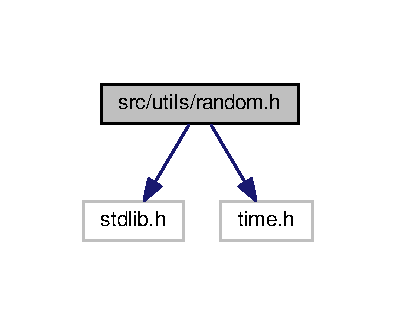
\includegraphics[width=190pt]{random_8h__incl}
\end{center}
\end{figure}
This graph shows which files directly or indirectly include this file\+:
\nopagebreak
\begin{figure}[H]
\begin{center}
\leavevmode
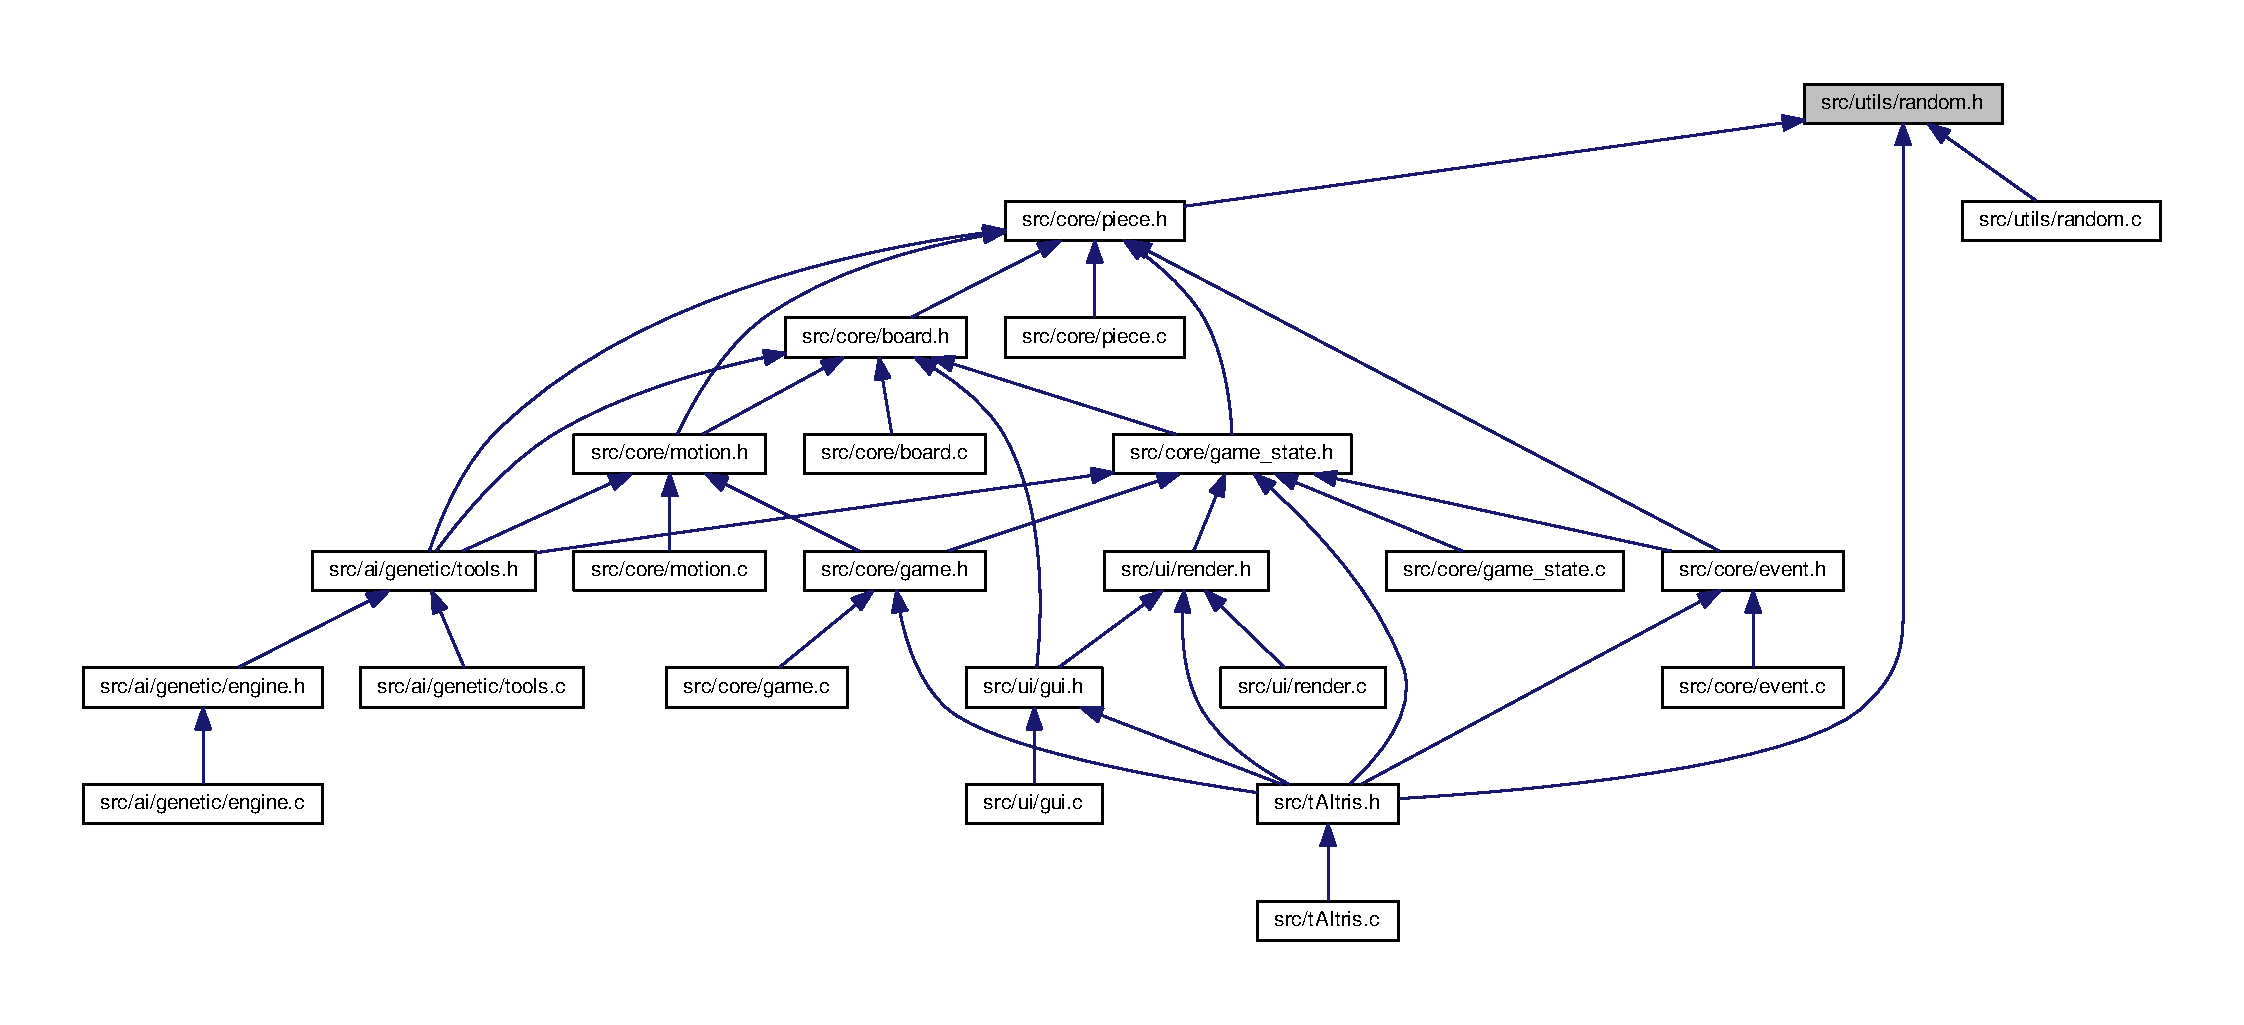
\includegraphics[width=350pt]{random_8h__dep__incl}
\end{center}
\end{figure}
\subsection*{Functions}
\begin{DoxyCompactItemize}
\item 
void \textbf{ random\+\_\+init} ()
\item 
size\+\_\+t \textbf{ random\+\_\+size\+\_\+t} (size\+\_\+t min, size\+\_\+t max)
\item 
int \textbf{ random\+\_\+int} (int min, int max)
\end{DoxyCompactItemize}


\subsection{Detailed Description}
No description. 

\begin{DoxyAuthor}{Author}
S4\+Master\+Race 
\end{DoxyAuthor}
\begin{DoxyVersion}{Version}
1.\+0 
\end{DoxyVersion}


\subsection{Function Documentation}
\mbox{\label{random_8h_af2e80b8de6ec1840dac4668ca5a38606}} 
\index{random.\+h@{random.\+h}!random\+\_\+init@{random\+\_\+init}}
\index{random\+\_\+init@{random\+\_\+init}!random.\+h@{random.\+h}}
\subsubsection{random\+\_\+init()}
{\footnotesize\ttfamily void random\+\_\+init (\begin{DoxyParamCaption}{ }\end{DoxyParamCaption})\hspace{0.3cm}{\ttfamily [inline]}}

\mbox{\label{random_8h_ad7954e6a1b9ea073c7bc894dc5af85a9}} 
\index{random.\+h@{random.\+h}!random\+\_\+int@{random\+\_\+int}}
\index{random\+\_\+int@{random\+\_\+int}!random.\+h@{random.\+h}}
\subsubsection{random\+\_\+int()}
{\footnotesize\ttfamily int random\+\_\+int (\begin{DoxyParamCaption}\item[{int}]{min,  }\item[{int}]{max }\end{DoxyParamCaption})\hspace{0.3cm}{\ttfamily [inline]}}

\mbox{\label{random_8h_a9911fe7c3f3108164ffac97c8d815142}} 
\index{random.\+h@{random.\+h}!random\+\_\+size\+\_\+t@{random\+\_\+size\+\_\+t}}
\index{random\+\_\+size\+\_\+t@{random\+\_\+size\+\_\+t}!random.\+h@{random.\+h}}
\subsubsection{random\+\_\+size\+\_\+t()}
{\footnotesize\ttfamily size\+\_\+t random\+\_\+size\+\_\+t (\begin{DoxyParamCaption}\item[{size\+\_\+t}]{min,  }\item[{size\+\_\+t}]{max }\end{DoxyParamCaption})\hspace{0.3cm}{\ttfamily [inline]}}


\section{src/utils/safe\+\_\+op.h File Reference}
\label{safe__op_8h}\index{src/utils/safe\+\_\+op.\+h@{src/utils/safe\+\_\+op.\+h}}


Safe operations.  


{\ttfamily \#include $<$limits.\+h$>$}\newline
Include dependency graph for safe\+\_\+op.\+h\+:
\nopagebreak
\begin{figure}[H]
\begin{center}
\leavevmode
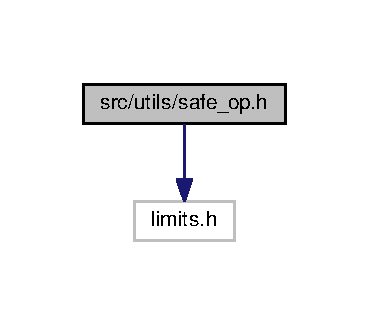
\includegraphics[width=177pt]{safe__op_8h__incl}
\end{center}
\end{figure}
This graph shows which files directly or indirectly include this file\+:
\nopagebreak
\begin{figure}[H]
\begin{center}
\leavevmode
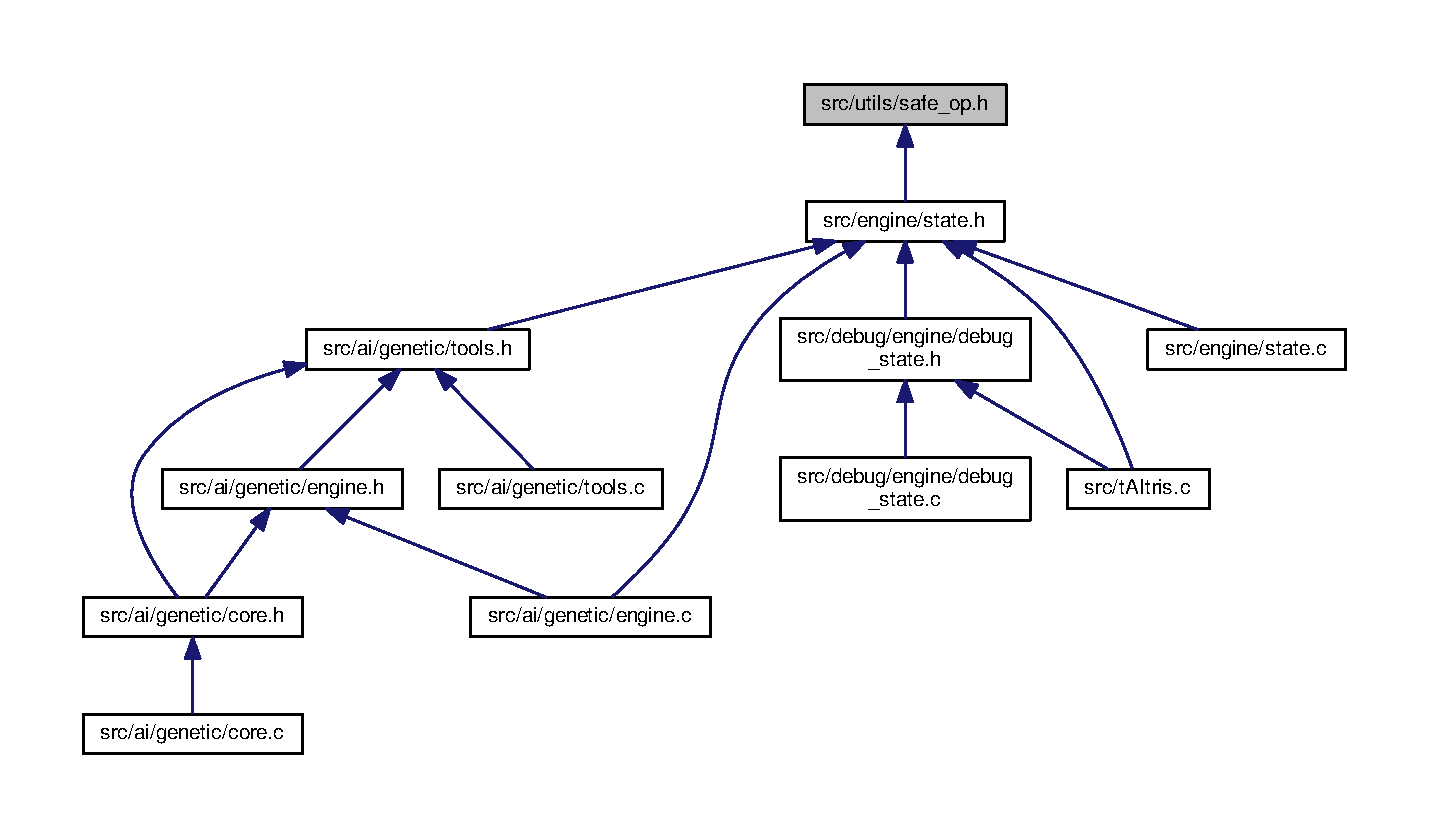
\includegraphics[width=350pt]{safe__op_8h__dep__incl}
\end{center}
\end{figure}
\subsection*{Macros}
\begin{DoxyCompactItemize}
\item 
\#define \textbf{ S\+A\+F\+E\+\_\+\+O\+P\+\_\+\+S\+U\+C\+C\+E\+SS}~0
\item 
\#define \textbf{ S\+A\+F\+E\+\_\+\+O\+P\+\_\+\+O\+V\+E\+R\+F\+L\+OW}~1
\item 
\#define \textbf{ S\+A\+F\+E\+\_\+\+O\+P\+\_\+\+U\+N\+D\+E\+R\+F\+L\+OW}~(-\/1)
\end{DoxyCompactItemize}


\subsection{Detailed Description}
Safe operations. 

\begin{DoxyAuthor}{Author}
S4\+Master\+Race 
\end{DoxyAuthor}
\begin{DoxyVersion}{Version}
2.\+0 
\end{DoxyVersion}


\subsection{Macro Definition Documentation}
\mbox{\label{safe__op_8h_aa0b22e9ac63f135e1a4238b40f68d571}} 
\index{safe\+\_\+op.\+h@{safe\+\_\+op.\+h}!S\+A\+F\+E\+\_\+\+O\+P\+\_\+\+O\+V\+E\+R\+F\+L\+OW@{S\+A\+F\+E\+\_\+\+O\+P\+\_\+\+O\+V\+E\+R\+F\+L\+OW}}
\index{S\+A\+F\+E\+\_\+\+O\+P\+\_\+\+O\+V\+E\+R\+F\+L\+OW@{S\+A\+F\+E\+\_\+\+O\+P\+\_\+\+O\+V\+E\+R\+F\+L\+OW}!safe\+\_\+op.\+h@{safe\+\_\+op.\+h}}
\subsubsection{S\+A\+F\+E\+\_\+\+O\+P\+\_\+\+O\+V\+E\+R\+F\+L\+OW}
{\footnotesize\ttfamily \#define S\+A\+F\+E\+\_\+\+O\+P\+\_\+\+O\+V\+E\+R\+F\+L\+OW~1}

\mbox{\label{safe__op_8h_a19408539e6669a9a14a03e03e2bcb436}} 
\index{safe\+\_\+op.\+h@{safe\+\_\+op.\+h}!S\+A\+F\+E\+\_\+\+O\+P\+\_\+\+S\+U\+C\+C\+E\+SS@{S\+A\+F\+E\+\_\+\+O\+P\+\_\+\+S\+U\+C\+C\+E\+SS}}
\index{S\+A\+F\+E\+\_\+\+O\+P\+\_\+\+S\+U\+C\+C\+E\+SS@{S\+A\+F\+E\+\_\+\+O\+P\+\_\+\+S\+U\+C\+C\+E\+SS}!safe\+\_\+op.\+h@{safe\+\_\+op.\+h}}
\subsubsection{S\+A\+F\+E\+\_\+\+O\+P\+\_\+\+S\+U\+C\+C\+E\+SS}
{\footnotesize\ttfamily \#define S\+A\+F\+E\+\_\+\+O\+P\+\_\+\+S\+U\+C\+C\+E\+SS~0}

\mbox{\label{safe__op_8h_ae529686976842c0d190204eaed573bcd}} 
\index{safe\+\_\+op.\+h@{safe\+\_\+op.\+h}!S\+A\+F\+E\+\_\+\+O\+P\+\_\+\+U\+N\+D\+E\+R\+F\+L\+OW@{S\+A\+F\+E\+\_\+\+O\+P\+\_\+\+U\+N\+D\+E\+R\+F\+L\+OW}}
\index{S\+A\+F\+E\+\_\+\+O\+P\+\_\+\+U\+N\+D\+E\+R\+F\+L\+OW@{S\+A\+F\+E\+\_\+\+O\+P\+\_\+\+U\+N\+D\+E\+R\+F\+L\+OW}!safe\+\_\+op.\+h@{safe\+\_\+op.\+h}}
\subsubsection{S\+A\+F\+E\+\_\+\+O\+P\+\_\+\+U\+N\+D\+E\+R\+F\+L\+OW}
{\footnotesize\ttfamily \#define S\+A\+F\+E\+\_\+\+O\+P\+\_\+\+U\+N\+D\+E\+R\+F\+L\+OW~(-\/1)}


%--- End generated contents ---

% Index
\backmatter
\newpage
\phantomsection
\clearemptydoublepage
\addcontentsline{toc}{chapter}{Index}
\printindex

\end{document}
